\RequirePackage{silence} % :-\
    \WarningFilter{scrreprt}{Usage of package `titlesec'}
    %\WarningFilter{scrreprt}{Activating an ugly workaround}
    \WarningFilter{titlesec}{Non standard sectioning command detected}
\documentclass[ twoside,openright,titlepage,numbers=noenddot,%1headlines,
                headinclude,footinclude,cleardoublepage=empty,abstract=on,
                BCOR=5mm,paper=a4,fontsize=11pt
                ]{scrreprt}

%********************************************************************
% Note: Make all your adjustments in here
%*******************************************************
% ****************************************************************************************************
% classicthesis-config.tex
% formerly known as loadpackages.sty, classicthesis-ldpkg.sty, and classicthesis-preamble.sty
% Use it at the beginning of your ClassicThesis.tex, or as a LaTeX Preamble
% in your ClassicThesis.{tex,lyx} with % ****************************************************************************************************
% classicthesis-config.tex
% formerly known as loadpackages.sty, classicthesis-ldpkg.sty, and classicthesis-preamble.sty
% Use it at the beginning of your ClassicThesis.tex, or as a LaTeX Preamble
% in your ClassicThesis.{tex,lyx} with % ****************************************************************************************************
% classicthesis-config.tex
% formerly known as loadpackages.sty, classicthesis-ldpkg.sty, and classicthesis-preamble.sty
% Use it at the beginning of your ClassicThesis.tex, or as a LaTeX Preamble
% in your ClassicThesis.{tex,lyx} with \input{classicthesis-config}
% ****************************************************************************************************
% If you like the classicthesis, then I would appreciate a postcard.
% My address can be found in the file ClassicThesis.pdf. A collection
% of the postcards I received so far is available online at
% http://postcards.miede.de
% ****************************************************************************************************


% ****************************************************************************************************
% 0. Set the encoding of your files. UTF-8 is the only sensible encoding nowadays. If you can't read
% äöüßáéçèê∂åëæƒÏ€ then change the encoding setting in your editor, not the line below. If your editor
% does not support utf8 use another editor!
% ****************************************************************************************************
\PassOptionsToPackage{utf8}{inputenc}
  \usepackage{inputenc}

\PassOptionsToPackage{T1}{fontenc} % T2A for cyrillics
  \usepackage{fontenc}


% ****************************************************************************************************
% 1. Configure classicthesis for your needs here, e.g., remove "drafting" below
% in order to deactivate the time-stamp on the pages
% (see ClassicThesis.pdf for more information):
% ****************************************************************************************************
\PassOptionsToPackage{
  drafting=false,    % print version information on the bottom of the pages
  tocaligned=false, % the left column of the toc will be aligned (no indentation)
  dottedtoc=false,  % page numbers in ToC flushed right
  eulerchapternumbers=true, % use AMS Euler for chapter font (otherwise Palatino)
  linedheaders=false,       % chaper headers will have line above and beneath
  floatperchapter=true,     % numbering per chapter for all floats (i.e., Figure 1.1)
  eulermath=false,  % use awesome Euler fonts for mathematical formulae (only with pdfLaTeX)
  beramono=true,    % toggle a nice monospaced font (w/ bold)
  palatino=true,    % deactivate standard font for loading another one, see the last section at the end of this file for suggestions
  style=classicthesis % classicthesis, arsclassica
}{classicthesis}


% ****************************************************************************************************
% 2. Personal data and user ad-hoc commands (insert your own data here)
% ****************************************************************************************************
\newcommand{\myTitle}{General Relativity\xspace}
\newcommand{\mySubtitle}{An Homage to The Elements of Typographic Style\xspace}
\newcommand{\myDegree}{Doktor-Ingenieur (Dr.-Ing.)\xspace}
\newcommand{\myName}{Thimo Preis\xspace}
\newcommand{\myProf}{Put name here\xspace}
\newcommand{\myOtherProf}{Put name here\xspace}
\newcommand{\mySupervisor}{Put name here\xspace}
\newcommand{\myFaculty}{Put data here\xspace}
\newcommand{\myDepartment}{Put data here\xspace}
\newcommand{\myUni}{Put data here\xspace}
\newcommand{\myLocation}{Saarbrücken\xspace}
\newcommand{\myTime}{ \today \xspace}
\newcommand{\myVersion}{\classicthesis}
\newcommand{\myEmail}{\href{mailto:preis@stud.uni-heidelberg.de}{preis@stud.uni-heidelberg.de}}
% ********************************************************************
% Setup, finetuning, and useful commands
% ********************************************************************
\providecommand{\mLyX}{L\kern-.1667em\lower.25em\hbox{Y}\kern-.125emX\@}
\newcommand{\ie}{i.\,e.}
\newcommand{\Ie}{I.\,e.}
\newcommand{\eg}{e.\,g.}
\newcommand{\Eg}{E.\,g.}
% ****************************************************************************************************


% ****************************************************************************************************
% 3. Loading some handy packages
% ****************************************************************************************************
% ********************************************************************
% Packages with options that might require adjustments
% ********************************************************************
\PassOptionsToPackage{ngerman,american, british}{babel} % change this to your language(s), main language last
% Spanish languages need extra options in order to work with this template
%\PassOptionsToPackage{spanish,es-lcroman}{babel}
    \usepackage{babel}

\usepackage{csquotes}
\PassOptionsToPackage{%
  %backend=biber,bibencoding=utf8, %instead of bibtex
  backend=bibtex8,bibencoding=ascii,%
  language=auto,%
  style=numeric-comp,%
  %style=authoryear-comp, % Author 1999, 2010
  %bibstyle=authoryear,dashed=false, % dashed: substitute rep. author with ---
  sorting=nyt, % name, year, title
  maxbibnames=10, % default: 3, et al.
  %backref=true,%
  natbib=true % natbib compatibility mode (\citep and \citet still work)
}{biblatex}
    \usepackage{biblatex}

\PassOptionsToPackage{fleqn}{amsmath}       % math environments and more by the AMS
  \usepackage{amsmath}

% ********************************************************************
% General useful packages
% ********************************************************************
\usepackage{graphicx} %
\usepackage{scrhack} % fix warnings when using KOMA with listings package
\usepackage{xspace} % to get the spacing after macros right
\PassOptionsToPackage{printonlyused,smaller}{acronym}
  \usepackage{acronym} % nice macros for handling all acronyms in the thesis
  %\renewcommand{\bflabel}[1]{{#1}\hfill} % fix the list of acronyms --> no longer working
  %\renewcommand*{\acsfont}[1]{\textsc{#1}}
  %\renewcommand*{\aclabelfont}[1]{\acsfont{#1}}
  %\def\bflabel#1{{#1\hfill}}
  \def\bflabel#1{{\acsfont{#1}\hfill}}
  \def\aclabelfont#1{\acsfont{#1}}
% ****************************************************************************************************
%\usepackage{pgfplots} % External TikZ/PGF support (thanks to Andreas Nautsch)
%\usetikzlibrary{external}
%\tikzexternalize[mode=list and make, prefix=ext-tikz/]
% ****************************************************************************************************


% ****************************************************************************************************
% 4. Setup floats: tables, (sub)figures, and captions
% ****************************************************************************************************
\usepackage{tabularx} % better tables
  \setlength{\extrarowheight}{3pt} % increase table row height
\newcommand{\tableheadline}[1]{\multicolumn{1}{l}{\spacedlowsmallcaps{#1}}}
\newcommand{\myfloatalign}{\centering} % to be used with each float for alignment
\usepackage{subfig}
% ****************************************************************************************************


% ****************************************************************************************************
% 5. Setup code listings
% ****************************************************************************************************
\usepackage{listings}
%\lstset{emph={trueIndex,root},emphstyle=\color{BlueViolet}}%\underbar} % for special keywords
\lstset{language=[LaTeX]Tex,%C++,
  morekeywords={PassOptionsToPackage,selectlanguage},
  keywordstyle=\color{RoyalBlue},%\bfseries,
  basicstyle=\small\ttfamily,
  %identifierstyle=\color{NavyBlue},
  commentstyle=\color{Green}\ttfamily,
  stringstyle=\rmfamily,
  numbers=none,%left,%
  numberstyle=\scriptsize,%\tiny
  stepnumber=5,
  numbersep=8pt,
  showstringspaces=false,
  breaklines=true,
  %frameround=ftff,
  %frame=single,
  belowcaptionskip=.75\baselineskip
  %frame=L
}
% ****************************************************************************************************




% ****************************************************************************************************
% 6. Last calls before the bar closes
% ****************************************************************************************************
% ********************************************************************
% Her Majesty herself
% ********************************************************************
\usepackage{classicthesis}


% ********************************************************************
% Fine-tune hyperreferences (hyperref should be called last)
% ********************************************************************
\hypersetup{%
  %draft, % hyperref's draft mode, for printing see below
  colorlinks=true, linktocpage=true, pdfstartpage=3, pdfstartview=FitV,%
  % uncomment the following line if you want to have black links (e.g., for printing)
  %colorlinks=false, linktocpage=false, pdfstartpage=3, pdfstartview=FitV, pdfborder={0 0 0},%
  breaklinks=true, pageanchor=true,%
  pdfpagemode=UseNone, %
  % pdfpagemode=UseOutlines,%
  plainpages=false, bookmarksnumbered, bookmarksopen=true, bookmarksopenlevel=1,%
  hypertexnames=true, pdfhighlight=/O,%nesting=true,%frenchlinks,%
  urlcolor=CTurl, linkcolor=CTlink, citecolor=CTcitation, %pagecolor=RoyalBlue,%
  %urlcolor=Black, linkcolor=Black, citecolor=Black, %pagecolor=Black,%
  pdftitle={\myTitle},%
  pdfauthor={\textcopyright\ \myName, \myUni, \myFaculty},%
  pdfsubject={},%
  pdfkeywords={},%
  pdfcreator={pdfLaTeX},%
  pdfproducer={LaTeX with hyperref and classicthesis}%
}


% ********************************************************************
% Setup autoreferences (hyperref and babel)
% ********************************************************************
% There are some issues regarding autorefnames
% http://www.tex.ac.uk/cgi-bin/texfaq2html?label=latexwords
% you have to redefine the macros for the
% language you use, e.g., american, ngerman
% (as chosen when loading babel/AtBeginDocument)
% ********************************************************************
\makeatletter
\@ifpackageloaded{babel}%
  {%
    \addto\extrasamerican{%
      \renewcommand*{\figureautorefname}{Figure}%
      \renewcommand*{\tableautorefname}{Table}%
      \renewcommand*{\partautorefname}{Part}%
      \renewcommand*{\chapterautorefname}{Chapter}%
      \renewcommand*{\sectionautorefname}{Section}%
      \renewcommand*{\subsectionautorefname}{Section}%
      \renewcommand*{\subsubsectionautorefname}{Section}%
    }%
    \addto\extrasngerman{%
      \renewcommand*{\paragraphautorefname}{Absatz}%
      \renewcommand*{\subparagraphautorefname}{Unterabsatz}%
      \renewcommand*{\footnoteautorefname}{Fu\"snote}%
      \renewcommand*{\FancyVerbLineautorefname}{Zeile}%
      \renewcommand*{\theoremautorefname}{Theorem}%
      \renewcommand*{\appendixautorefname}{Anhang}%
      \renewcommand*{\equationautorefname}{Gleichung}%
      \renewcommand*{\itemautorefname}{Punkt}%
    }%
      % Fix to getting autorefs for subfigures right (thanks to Belinda Vogt for changing the definition)
      \providecommand{\subfigureautorefname}{\figureautorefname}%
    }{\relax}
\makeatother


% ********************************************************************
% Development Stuff
% ********************************************************************
\listfiles
%\PassOptionsToPackage{l2tabu,orthodox,abort}{nag}
%  \usepackage{nag}
%\PassOptionsToPackage{warning, all}{onlyamsmath}
%  \usepackage{onlyamsmath}


% ****************************************************************************************************
% 7. Further adjustments (experimental)
% ****************************************************************************************************
% ********************************************************************
% Changing the text area
% ********************************************************************
%\areaset[current]{312pt}{761pt} % 686 (factor 2.2) + 33 head + 42 head \the\footskip
%\setlength{\marginparwidth}{7em}%
%\setlength{\marginparsep}{2em}%

% ********************************************************************
% Using different fonts
% ********************************************************************
%\usepackage[oldstylenums]{kpfonts} % oldstyle notextcomp
% \usepackage[osf]{libertine}
%\usepackage[light,condensed,math]{iwona}
%\renewcommand{\sfdefault}{iwona}
%\usepackage{lmodern} % <-- no osf support :-(
%\usepackage{cfr-lm} %
%\usepackage[urw-garamond]{mathdesign} <-- no osf support :-(
%\usepackage[default,osfigures]{opensans} % scale=0.95
%\usepackage[sfdefault]{FiraSans}
% \usepackage[opticals,mathlf]{MinionPro} % onlytext
% ********************************************************************
%\usepackage[largesc,osf]{newpxtext}
%\linespread{1.05} % a bit more for Palatino
% Used to fix these:
% https://bitbucket.org/amiede/classicthesis/issues/139/italics-in-pallatino-capitals-chapter
% https://bitbucket.org/amiede/classicthesis/issues/45/problema-testatine-su-classicthesis-style
% ********************************************************************
% ****************************************************************************************************

% ****************************************************************************************************
% If you like the classicthesis, then I would appreciate a postcard.
% My address can be found in the file ClassicThesis.pdf. A collection
% of the postcards I received so far is available online at
% http://postcards.miede.de
% ****************************************************************************************************


% ****************************************************************************************************
% 0. Set the encoding of your files. UTF-8 is the only sensible encoding nowadays. If you can't read
% äöüßáéçèê∂åëæƒÏ€ then change the encoding setting in your editor, not the line below. If your editor
% does not support utf8 use another editor!
% ****************************************************************************************************
\PassOptionsToPackage{utf8}{inputenc}
  \usepackage{inputenc}

\PassOptionsToPackage{T1}{fontenc} % T2A for cyrillics
  \usepackage{fontenc}


% ****************************************************************************************************
% 1. Configure classicthesis for your needs here, e.g., remove "drafting" below
% in order to deactivate the time-stamp on the pages
% (see ClassicThesis.pdf for more information):
% ****************************************************************************************************
\PassOptionsToPackage{
  drafting=false,    % print version information on the bottom of the pages
  tocaligned=false, % the left column of the toc will be aligned (no indentation)
  dottedtoc=false,  % page numbers in ToC flushed right
  eulerchapternumbers=true, % use AMS Euler for chapter font (otherwise Palatino)
  linedheaders=false,       % chaper headers will have line above and beneath
  floatperchapter=true,     % numbering per chapter for all floats (i.e., Figure 1.1)
  eulermath=false,  % use awesome Euler fonts for mathematical formulae (only with pdfLaTeX)
  beramono=true,    % toggle a nice monospaced font (w/ bold)
  palatino=true,    % deactivate standard font for loading another one, see the last section at the end of this file for suggestions
  style=classicthesis % classicthesis, arsclassica
}{classicthesis}


% ****************************************************************************************************
% 2. Personal data and user ad-hoc commands (insert your own data here)
% ****************************************************************************************************
\newcommand{\myTitle}{General Relativity\xspace}
\newcommand{\mySubtitle}{An Homage to The Elements of Typographic Style\xspace}
\newcommand{\myDegree}{Doktor-Ingenieur (Dr.-Ing.)\xspace}
\newcommand{\myName}{Thimo Preis\xspace}
\newcommand{\myProf}{Put name here\xspace}
\newcommand{\myOtherProf}{Put name here\xspace}
\newcommand{\mySupervisor}{Put name here\xspace}
\newcommand{\myFaculty}{Put data here\xspace}
\newcommand{\myDepartment}{Put data here\xspace}
\newcommand{\myUni}{Put data here\xspace}
\newcommand{\myLocation}{Saarbrücken\xspace}
\newcommand{\myTime}{ \today \xspace}
\newcommand{\myVersion}{\classicthesis}
\newcommand{\myEmail}{\href{mailto:preis@stud.uni-heidelberg.de}{preis@stud.uni-heidelberg.de}}
% ********************************************************************
% Setup, finetuning, and useful commands
% ********************************************************************
\providecommand{\mLyX}{L\kern-.1667em\lower.25em\hbox{Y}\kern-.125emX\@}
\newcommand{\ie}{i.\,e.}
\newcommand{\Ie}{I.\,e.}
\newcommand{\eg}{e.\,g.}
\newcommand{\Eg}{E.\,g.}
% ****************************************************************************************************


% ****************************************************************************************************
% 3. Loading some handy packages
% ****************************************************************************************************
% ********************************************************************
% Packages with options that might require adjustments
% ********************************************************************
\PassOptionsToPackage{ngerman,american, british}{babel} % change this to your language(s), main language last
% Spanish languages need extra options in order to work with this template
%\PassOptionsToPackage{spanish,es-lcroman}{babel}
    \usepackage{babel}

\usepackage{csquotes}
\PassOptionsToPackage{%
  %backend=biber,bibencoding=utf8, %instead of bibtex
  backend=bibtex8,bibencoding=ascii,%
  language=auto,%
  style=numeric-comp,%
  %style=authoryear-comp, % Author 1999, 2010
  %bibstyle=authoryear,dashed=false, % dashed: substitute rep. author with ---
  sorting=nyt, % name, year, title
  maxbibnames=10, % default: 3, et al.
  %backref=true,%
  natbib=true % natbib compatibility mode (\citep and \citet still work)
}{biblatex}
    \usepackage{biblatex}

\PassOptionsToPackage{fleqn}{amsmath}       % math environments and more by the AMS
  \usepackage{amsmath}

% ********************************************************************
% General useful packages
% ********************************************************************
\usepackage{graphicx} %
\usepackage{scrhack} % fix warnings when using KOMA with listings package
\usepackage{xspace} % to get the spacing after macros right
\PassOptionsToPackage{printonlyused,smaller}{acronym}
  \usepackage{acronym} % nice macros for handling all acronyms in the thesis
  %\renewcommand{\bflabel}[1]{{#1}\hfill} % fix the list of acronyms --> no longer working
  %\renewcommand*{\acsfont}[1]{\textsc{#1}}
  %\renewcommand*{\aclabelfont}[1]{\acsfont{#1}}
  %\def\bflabel#1{{#1\hfill}}
  \def\bflabel#1{{\acsfont{#1}\hfill}}
  \def\aclabelfont#1{\acsfont{#1}}
% ****************************************************************************************************
%\usepackage{pgfplots} % External TikZ/PGF support (thanks to Andreas Nautsch)
%\usetikzlibrary{external}
%\tikzexternalize[mode=list and make, prefix=ext-tikz/]
% ****************************************************************************************************


% ****************************************************************************************************
% 4. Setup floats: tables, (sub)figures, and captions
% ****************************************************************************************************
\usepackage{tabularx} % better tables
  \setlength{\extrarowheight}{3pt} % increase table row height
\newcommand{\tableheadline}[1]{\multicolumn{1}{l}{\spacedlowsmallcaps{#1}}}
\newcommand{\myfloatalign}{\centering} % to be used with each float for alignment
\usepackage{subfig}
% ****************************************************************************************************


% ****************************************************************************************************
% 5. Setup code listings
% ****************************************************************************************************
\usepackage{listings}
%\lstset{emph={trueIndex,root},emphstyle=\color{BlueViolet}}%\underbar} % for special keywords
\lstset{language=[LaTeX]Tex,%C++,
  morekeywords={PassOptionsToPackage,selectlanguage},
  keywordstyle=\color{RoyalBlue},%\bfseries,
  basicstyle=\small\ttfamily,
  %identifierstyle=\color{NavyBlue},
  commentstyle=\color{Green}\ttfamily,
  stringstyle=\rmfamily,
  numbers=none,%left,%
  numberstyle=\scriptsize,%\tiny
  stepnumber=5,
  numbersep=8pt,
  showstringspaces=false,
  breaklines=true,
  %frameround=ftff,
  %frame=single,
  belowcaptionskip=.75\baselineskip
  %frame=L
}
% ****************************************************************************************************




% ****************************************************************************************************
% 6. Last calls before the bar closes
% ****************************************************************************************************
% ********************************************************************
% Her Majesty herself
% ********************************************************************
\usepackage{classicthesis}


% ********************************************************************
% Fine-tune hyperreferences (hyperref should be called last)
% ********************************************************************
\hypersetup{%
  %draft, % hyperref's draft mode, for printing see below
  colorlinks=true, linktocpage=true, pdfstartpage=3, pdfstartview=FitV,%
  % uncomment the following line if you want to have black links (e.g., for printing)
  %colorlinks=false, linktocpage=false, pdfstartpage=3, pdfstartview=FitV, pdfborder={0 0 0},%
  breaklinks=true, pageanchor=true,%
  pdfpagemode=UseNone, %
  % pdfpagemode=UseOutlines,%
  plainpages=false, bookmarksnumbered, bookmarksopen=true, bookmarksopenlevel=1,%
  hypertexnames=true, pdfhighlight=/O,%nesting=true,%frenchlinks,%
  urlcolor=CTurl, linkcolor=CTlink, citecolor=CTcitation, %pagecolor=RoyalBlue,%
  %urlcolor=Black, linkcolor=Black, citecolor=Black, %pagecolor=Black,%
  pdftitle={\myTitle},%
  pdfauthor={\textcopyright\ \myName, \myUni, \myFaculty},%
  pdfsubject={},%
  pdfkeywords={},%
  pdfcreator={pdfLaTeX},%
  pdfproducer={LaTeX with hyperref and classicthesis}%
}


% ********************************************************************
% Setup autoreferences (hyperref and babel)
% ********************************************************************
% There are some issues regarding autorefnames
% http://www.tex.ac.uk/cgi-bin/texfaq2html?label=latexwords
% you have to redefine the macros for the
% language you use, e.g., american, ngerman
% (as chosen when loading babel/AtBeginDocument)
% ********************************************************************
\makeatletter
\@ifpackageloaded{babel}%
  {%
    \addto\extrasamerican{%
      \renewcommand*{\figureautorefname}{Figure}%
      \renewcommand*{\tableautorefname}{Table}%
      \renewcommand*{\partautorefname}{Part}%
      \renewcommand*{\chapterautorefname}{Chapter}%
      \renewcommand*{\sectionautorefname}{Section}%
      \renewcommand*{\subsectionautorefname}{Section}%
      \renewcommand*{\subsubsectionautorefname}{Section}%
    }%
    \addto\extrasngerman{%
      \renewcommand*{\paragraphautorefname}{Absatz}%
      \renewcommand*{\subparagraphautorefname}{Unterabsatz}%
      \renewcommand*{\footnoteautorefname}{Fu\"snote}%
      \renewcommand*{\FancyVerbLineautorefname}{Zeile}%
      \renewcommand*{\theoremautorefname}{Theorem}%
      \renewcommand*{\appendixautorefname}{Anhang}%
      \renewcommand*{\equationautorefname}{Gleichung}%
      \renewcommand*{\itemautorefname}{Punkt}%
    }%
      % Fix to getting autorefs for subfigures right (thanks to Belinda Vogt for changing the definition)
      \providecommand{\subfigureautorefname}{\figureautorefname}%
    }{\relax}
\makeatother


% ********************************************************************
% Development Stuff
% ********************************************************************
\listfiles
%\PassOptionsToPackage{l2tabu,orthodox,abort}{nag}
%  \usepackage{nag}
%\PassOptionsToPackage{warning, all}{onlyamsmath}
%  \usepackage{onlyamsmath}


% ****************************************************************************************************
% 7. Further adjustments (experimental)
% ****************************************************************************************************
% ********************************************************************
% Changing the text area
% ********************************************************************
%\areaset[current]{312pt}{761pt} % 686 (factor 2.2) + 33 head + 42 head \the\footskip
%\setlength{\marginparwidth}{7em}%
%\setlength{\marginparsep}{2em}%

% ********************************************************************
% Using different fonts
% ********************************************************************
%\usepackage[oldstylenums]{kpfonts} % oldstyle notextcomp
% \usepackage[osf]{libertine}
%\usepackage[light,condensed,math]{iwona}
%\renewcommand{\sfdefault}{iwona}
%\usepackage{lmodern} % <-- no osf support :-(
%\usepackage{cfr-lm} %
%\usepackage[urw-garamond]{mathdesign} <-- no osf support :-(
%\usepackage[default,osfigures]{opensans} % scale=0.95
%\usepackage[sfdefault]{FiraSans}
% \usepackage[opticals,mathlf]{MinionPro} % onlytext
% ********************************************************************
%\usepackage[largesc,osf]{newpxtext}
%\linespread{1.05} % a bit more for Palatino
% Used to fix these:
% https://bitbucket.org/amiede/classicthesis/issues/139/italics-in-pallatino-capitals-chapter
% https://bitbucket.org/amiede/classicthesis/issues/45/problema-testatine-su-classicthesis-style
% ********************************************************************
% ****************************************************************************************************

% ****************************************************************************************************
% If you like the classicthesis, then I would appreciate a postcard.
% My address can be found in the file ClassicThesis.pdf. A collection
% of the postcards I received so far is available online at
% http://postcards.miede.de
% ****************************************************************************************************


% ****************************************************************************************************
% 0. Set the encoding of your files. UTF-8 is the only sensible encoding nowadays. If you can't read
% äöüßáéçèê∂åëæƒÏ€ then change the encoding setting in your editor, not the line below. If your editor
% does not support utf8 use another editor!
% ****************************************************************************************************
\PassOptionsToPackage{utf8}{inputenc}
  \usepackage{inputenc}

\PassOptionsToPackage{T1}{fontenc} % T2A for cyrillics
  \usepackage{fontenc}


% ****************************************************************************************************
% 1. Configure classicthesis for your needs here, e.g., remove "drafting" below
% in order to deactivate the time-stamp on the pages
% (see ClassicThesis.pdf for more information):
% ****************************************************************************************************
\PassOptionsToPackage{
  drafting=false,    % print version information on the bottom of the pages
  tocaligned=false, % the left column of the toc will be aligned (no indentation)
  dottedtoc=false,  % page numbers in ToC flushed right
  eulerchapternumbers=true, % use AMS Euler for chapter font (otherwise Palatino)
  linedheaders=false,       % chaper headers will have line above and beneath
  floatperchapter=true,     % numbering per chapter for all floats (i.e., Figure 1.1)
  eulermath=false,  % use awesome Euler fonts for mathematical formulae (only with pdfLaTeX)
  beramono=true,    % toggle a nice monospaced font (w/ bold)
  palatino=true,    % deactivate standard font for loading another one, see the last section at the end of this file for suggestions
  style=classicthesis % classicthesis, arsclassica
}{classicthesis}


% ****************************************************************************************************
% 2. Personal data and user ad-hoc commands (insert your own data here)
% ****************************************************************************************************
\newcommand{\myTitle}{General Relativity\xspace}
\newcommand{\mySubtitle}{An Homage to The Elements of Typographic Style\xspace}
\newcommand{\myDegree}{Doktor-Ingenieur (Dr.-Ing.)\xspace}
\newcommand{\myName}{Thimo Preis\xspace}
\newcommand{\myProf}{Put name here\xspace}
\newcommand{\myOtherProf}{Put name here\xspace}
\newcommand{\mySupervisor}{Put name here\xspace}
\newcommand{\myFaculty}{Put data here\xspace}
\newcommand{\myDepartment}{Put data here\xspace}
\newcommand{\myUni}{Put data here\xspace}
\newcommand{\myLocation}{Saarbrücken\xspace}
\newcommand{\myTime}{ \today \xspace}
\newcommand{\myVersion}{\classicthesis}
\newcommand{\myEmail}{\href{mailto:preis@stud.uni-heidelberg.de}{preis@stud.uni-heidelberg.de}}
% ********************************************************************
% Setup, finetuning, and useful commands
% ********************************************************************
\providecommand{\mLyX}{L\kern-.1667em\lower.25em\hbox{Y}\kern-.125emX\@}
\newcommand{\ie}{i.\,e.}
\newcommand{\Ie}{I.\,e.}
\newcommand{\eg}{e.\,g.}
\newcommand{\Eg}{E.\,g.}
% ****************************************************************************************************


% ****************************************************************************************************
% 3. Loading some handy packages
% ****************************************************************************************************
% ********************************************************************
% Packages with options that might require adjustments
% ********************************************************************
\PassOptionsToPackage{ngerman,american, british}{babel} % change this to your language(s), main language last
% Spanish languages need extra options in order to work with this template
%\PassOptionsToPackage{spanish,es-lcroman}{babel}
    \usepackage{babel}

\usepackage{csquotes}
\PassOptionsToPackage{%
  %backend=biber,bibencoding=utf8, %instead of bibtex
  backend=bibtex8,bibencoding=ascii,%
  language=auto,%
  style=numeric-comp,%
  %style=authoryear-comp, % Author 1999, 2010
  %bibstyle=authoryear,dashed=false, % dashed: substitute rep. author with ---
  sorting=nyt, % name, year, title
  maxbibnames=10, % default: 3, et al.
  %backref=true,%
  natbib=true % natbib compatibility mode (\citep and \citet still work)
}{biblatex}
    \usepackage{biblatex}

\PassOptionsToPackage{fleqn}{amsmath}       % math environments and more by the AMS
  \usepackage{amsmath}

% ********************************************************************
% General useful packages
% ********************************************************************
\usepackage{graphicx} %
\usepackage{scrhack} % fix warnings when using KOMA with listings package
\usepackage{xspace} % to get the spacing after macros right
\PassOptionsToPackage{printonlyused,smaller}{acronym}
  \usepackage{acronym} % nice macros for handling all acronyms in the thesis
  %\renewcommand{\bflabel}[1]{{#1}\hfill} % fix the list of acronyms --> no longer working
  %\renewcommand*{\acsfont}[1]{\textsc{#1}}
  %\renewcommand*{\aclabelfont}[1]{\acsfont{#1}}
  %\def\bflabel#1{{#1\hfill}}
  \def\bflabel#1{{\acsfont{#1}\hfill}}
  \def\aclabelfont#1{\acsfont{#1}}
% ****************************************************************************************************
%\usepackage{pgfplots} % External TikZ/PGF support (thanks to Andreas Nautsch)
%\usetikzlibrary{external}
%\tikzexternalize[mode=list and make, prefix=ext-tikz/]
% ****************************************************************************************************


% ****************************************************************************************************
% 4. Setup floats: tables, (sub)figures, and captions
% ****************************************************************************************************
\usepackage{tabularx} % better tables
  \setlength{\extrarowheight}{3pt} % increase table row height
\newcommand{\tableheadline}[1]{\multicolumn{1}{l}{\spacedlowsmallcaps{#1}}}
\newcommand{\myfloatalign}{\centering} % to be used with each float for alignment
\usepackage{subfig}
% ****************************************************************************************************


% ****************************************************************************************************
% 5. Setup code listings
% ****************************************************************************************************
\usepackage{listings}
%\lstset{emph={trueIndex,root},emphstyle=\color{BlueViolet}}%\underbar} % for special keywords
\lstset{language=[LaTeX]Tex,%C++,
  morekeywords={PassOptionsToPackage,selectlanguage},
  keywordstyle=\color{RoyalBlue},%\bfseries,
  basicstyle=\small\ttfamily,
  %identifierstyle=\color{NavyBlue},
  commentstyle=\color{Green}\ttfamily,
  stringstyle=\rmfamily,
  numbers=none,%left,%
  numberstyle=\scriptsize,%\tiny
  stepnumber=5,
  numbersep=8pt,
  showstringspaces=false,
  breaklines=true,
  %frameround=ftff,
  %frame=single,
  belowcaptionskip=.75\baselineskip
  %frame=L
}
% ****************************************************************************************************




% ****************************************************************************************************
% 6. Last calls before the bar closes
% ****************************************************************************************************
% ********************************************************************
% Her Majesty herself
% ********************************************************************
\usepackage{classicthesis}


% ********************************************************************
% Fine-tune hyperreferences (hyperref should be called last)
% ********************************************************************
\hypersetup{%
  %draft, % hyperref's draft mode, for printing see below
  colorlinks=true, linktocpage=true, pdfstartpage=3, pdfstartview=FitV,%
  % uncomment the following line if you want to have black links (e.g., for printing)
  %colorlinks=false, linktocpage=false, pdfstartpage=3, pdfstartview=FitV, pdfborder={0 0 0},%
  breaklinks=true, pageanchor=true,%
  pdfpagemode=UseNone, %
  % pdfpagemode=UseOutlines,%
  plainpages=false, bookmarksnumbered, bookmarksopen=true, bookmarksopenlevel=1,%
  hypertexnames=true, pdfhighlight=/O,%nesting=true,%frenchlinks,%
  urlcolor=CTurl, linkcolor=CTlink, citecolor=CTcitation, %pagecolor=RoyalBlue,%
  %urlcolor=Black, linkcolor=Black, citecolor=Black, %pagecolor=Black,%
  pdftitle={\myTitle},%
  pdfauthor={\textcopyright\ \myName, \myUni, \myFaculty},%
  pdfsubject={},%
  pdfkeywords={},%
  pdfcreator={pdfLaTeX},%
  pdfproducer={LaTeX with hyperref and classicthesis}%
}


% ********************************************************************
% Setup autoreferences (hyperref and babel)
% ********************************************************************
% There are some issues regarding autorefnames
% http://www.tex.ac.uk/cgi-bin/texfaq2html?label=latexwords
% you have to redefine the macros for the
% language you use, e.g., american, ngerman
% (as chosen when loading babel/AtBeginDocument)
% ********************************************************************
\makeatletter
\@ifpackageloaded{babel}%
  {%
    \addto\extrasamerican{%
      \renewcommand*{\figureautorefname}{Figure}%
      \renewcommand*{\tableautorefname}{Table}%
      \renewcommand*{\partautorefname}{Part}%
      \renewcommand*{\chapterautorefname}{Chapter}%
      \renewcommand*{\sectionautorefname}{Section}%
      \renewcommand*{\subsectionautorefname}{Section}%
      \renewcommand*{\subsubsectionautorefname}{Section}%
    }%
    \addto\extrasngerman{%
      \renewcommand*{\paragraphautorefname}{Absatz}%
      \renewcommand*{\subparagraphautorefname}{Unterabsatz}%
      \renewcommand*{\footnoteautorefname}{Fu\"snote}%
      \renewcommand*{\FancyVerbLineautorefname}{Zeile}%
      \renewcommand*{\theoremautorefname}{Theorem}%
      \renewcommand*{\appendixautorefname}{Anhang}%
      \renewcommand*{\equationautorefname}{Gleichung}%
      \renewcommand*{\itemautorefname}{Punkt}%
    }%
      % Fix to getting autorefs for subfigures right (thanks to Belinda Vogt for changing the definition)
      \providecommand{\subfigureautorefname}{\figureautorefname}%
    }{\relax}
\makeatother


% ********************************************************************
% Development Stuff
% ********************************************************************
\listfiles
%\PassOptionsToPackage{l2tabu,orthodox,abort}{nag}
%  \usepackage{nag}
%\PassOptionsToPackage{warning, all}{onlyamsmath}
%  \usepackage{onlyamsmath}


% ****************************************************************************************************
% 7. Further adjustments (experimental)
% ****************************************************************************************************
% ********************************************************************
% Changing the text area
% ********************************************************************
%\areaset[current]{312pt}{761pt} % 686 (factor 2.2) + 33 head + 42 head \the\footskip
%\setlength{\marginparwidth}{7em}%
%\setlength{\marginparsep}{2em}%

% ********************************************************************
% Using different fonts
% ********************************************************************
%\usepackage[oldstylenums]{kpfonts} % oldstyle notextcomp
% \usepackage[osf]{libertine}
%\usepackage[light,condensed,math]{iwona}
%\renewcommand{\sfdefault}{iwona}
%\usepackage{lmodern} % <-- no osf support :-(
%\usepackage{cfr-lm} %
%\usepackage[urw-garamond]{mathdesign} <-- no osf support :-(
%\usepackage[default,osfigures]{opensans} % scale=0.95
%\usepackage[sfdefault]{FiraSans}
% \usepackage[opticals,mathlf]{MinionPro} % onlytext
% ********************************************************************
%\usepackage[largesc,osf]{newpxtext}
%\linespread{1.05} % a bit more for Palatino
% Used to fix these:
% https://bitbucket.org/amiede/classicthesis/issues/139/italics-in-pallatino-capitals-chapter
% https://bitbucket.org/amiede/classicthesis/issues/45/problema-testatine-su-classicthesis-style
% ********************************************************************
% ****************************************************************************************************

\setlength{\parindent}{0pt}
\usepackage[most]{tcolorbox}
\newtcolorbox{mybox}[1]{%
	tikznode boxed title,
	enhanced,
	arc=0mm,
	interior style={white},
	attach boxed title to top center= {yshift=-\tcboxedtitleheight/2},
	fonttitle=\bfseries,
	colbacktitle=white,coltitle=black,
	boxed title style={size=normal,colframe=white,boxrule=0pt},
	title={#1}}
\newcommand{\mR}{\mathbb{R}}
\newcommand{\mJ}{\mathcal{J}}
\newcommand{\md}{\mathrm{d}}
\newcommand{\tr}{\mathrm{Tr}}
\newcommand{\pmeasure}{\frac{\md^3 p}{(2 \pi)^3}}
 \usepackage{physics}
 \newcommand{\half}{\frac{1}{2}}
 \newcommand{\mL}{\mathcal{L}}
 \newcommand{\normord}[1]{\vcentcolon\mathrel{#1}\vcentcolon}
 \providecommand{\vcentcolon}{\mathrel{\mathop{:}}}
 \usepackage{simplewick}
 \usepackage[compat=1.1.0]{tikz-feynman}
 \newcommand{\mg}{\mathcal{g}}
 \usepackage{slashed}
 \newcommand{\munu}{_{\mu \nu}}
 \newcommand{\mG}{\mathcal{G}}
 \usepackage{savesym}
  \savesymbol{eth}
   \savesymbol{digamma}
    \savesymbol{backepsilon}
 \usepackage{amssymb}

 \restoresymbol{ams}{eth}
  \restoresymbol{ams}{digamma}
   \restoresymbol{ams}{backepsilon}
 
	%********************************************************************
% Bibliographies
%*******************************************************
\addbibresource{Bibliography.bib}
\addbibresource[label=ownpubs]{AMiede_Publications.bib}
%-----------------------------------------
%My packages
%------------------------------------------
\usepackage[hyperref]{ntheorem}
\newtheorem{statements}{Statements}[chapter]
\usepackage{todonotes}
\usepackage{tikz}
\usetikzlibrary{3d,calc,shapes.geometric}
\usepackage{caption}
\usepackage{frcursive}
\usepackage{soul}



%********************************************************************
% Hyphenation
%*******************************************************
%\hyphenation{put special hyphenation here}

% ********************************************************************
% GO!GO!GO! MOVE IT!
%*******************************************************
\begin{document}
\frenchspacing
\raggedbottom
\selectlanguage{british} % american ngerman
%\renewcommand*{\bibname}{new name}
%\setbibpreamble{}
\pagenumbering{roman}
\pagestyle{plain}
%********************************************************************
% Frontmatter
%*******************************************************

%*******************************************************
% Titlepage
%*******************************************************
\begin{titlepage}
    %\pdfbookmark[1]{\myTitle}{titlepage}
    % if you want the titlepage to be centered, uncomment and fine-tune the line below (KOMA classes environment)
    \begin{addmargin}[-1cm]{-3cm}
    \begin{center}
        \large

        \hfill

        \vfill

        \begingroup
            \color{CTtitle}\spacedallcaps{\myTitle} \\ \bigskip
        \endgroup

        \spacedlowsmallcaps{\myName}\footnote{\href{mailto:thimo.preis@posteo.de}{thimo.preis@posteo.de}}
        

        \vfill

        \myTime

        \vfill

    \end{center}
  \end{addmargin}
\end{titlepage}

\cleardoublepage%*******************************************************
% Table of Contents
%*******************************************************
\pagestyle{scrheadings}
%\phantomsection
\pdfbookmark[1]{\contentsname}{tableofcontents}
\setcounter{tocdepth}{2} % <-- 2 includes up to subsections in the ToC
\setcounter{secnumdepth}{3} % <-- 3 numbers up to subsubsections
\manualmark
\markboth{\spacedlowsmallcaps{\contentsname}}{\spacedlowsmallcaps{\contentsname}}
\tableofcontents
\automark[section]{chapter}
\renewcommand{\chaptermark}[1]{\markboth{\spacedlowsmallcaps{#1}}{\spacedlowsmallcaps{#1}}}
\renewcommand{\sectionmark}[1]{\markright{\textsc{\thesection}\enspace\spacedlowsmallcaps{#1}}}
%*******************************************************
% List of Figures and of the Tables
%*******************************************************
\clearpage
% \pagestyle{empty} % Uncomment this line if your lists should not have any headlines with section name and page number
\begingroup
    \let\clearpage\relax
    \let\cleardoublepage\relax
    %*******************************************************
    % List of Figures
    %*******************************************************
    %\phantomsection
    %\addcontentsline{toc}{chapter}{\listfigurename}
    \pdfbookmark[1]{\listfigurename}{lof}
    \listoffigures

    \vspace{8ex}

    %*******************************************************
    % List of Tables
    %*******************************************************
    %\phantomsection
    %\addcontentsline{toc}{chapter}{\listtablename}
    \pdfbookmark[1]{\listtablename}{lot}
    \listoftables

    \vspace{8ex}
    % \newpage

    %*******************************************************
    % List of Listings
    %*******************************************************
    %\phantomsection
    %\addcontentsline{toc}{chapter}{\lstlistlistingname}
    \pdfbookmark[1]{\lstlistlistingname}{lol}
    \lstlistoflistings

    \vspace{8ex}

    %*******************************************************
    % Acronyms
    %*******************************************************
    %\phantomsection
    \pdfbookmark[1]{Acronyms}{acronyms}
    \markboth{\spacedlowsmallcaps{Acronyms}}{\spacedlowsmallcaps{Acronyms}}
    \chapter*{Acronyms}
    \begin{acronym}[UMLX]
        \acro{DRY}{Don't Repeat Yourself}
        \acro{API}{Application Programming Interface}
        \acro{UML}{Unified Modeling Language}
    \end{acronym}

\endgroup

%********************************************************************
% Mainmatter
%*******************************************************
\cleardoublepage
\pagestyle{scrheadings}
\pagenumbering{arabic}
%\setcounter{page}{90}
% use \cleardoublepage here to avoid problems with pdfbookmark
\cleardoublepage
\listoftodos

\newpage
\section*{Acknowledgements}

This is a compilation of lectures (most importantly by Prof. Bartelmann in the summer of $2019$) I attended and books (mostly "Cosmology" by Weinberg) I read on the topic of General Relativity, Differential Geometry, Theoretical Astrophysics and Cosmology.\\
\\
If you find any typos, feel free to send them to me \href{mailto:preis@stud.uni-heidelberg.de}{preis@stud.uni-heidelberg.de}. I do not claim originality of the content presented here, as It is heavily inspired by and drawn from various sources.
\\
\\
These notes are currently a work in progress, so for updated notes, as well as a list of other notes/works I have available, visit my web site

\begin{center}
    \href{thpreis.github.io}{thpreis.github.io}
\end{center}
\vspace{1cm}

\begin{flushright}
    \Huge{{\cursive\setul{0.1ex}{}\ul{~~Thimo Preis~~}}}
\end{flushright}

\chapter{Differential Geomtry}
\label{ch:diffgeo}
\section{Differentiable manifolds}
What we refer to as \emph{spacetime} is simply a set of points that each refers to an event in our
Universe. A supplementary topology establishes a notion of continuity on this set. We
further require that we may chart overlapping patches of our Universe, associating a set
of coordinates to each event, to arrive at the mathematical construct of a manifold. The
number of coordinates necessary for a chart of our Universe corresponds to its spacetime
dimension. The specific choice of coordinates is entirely up to us, however, and cannot
have any implications on the physical processes. Therefore, there are a priori no universal
notions of space and time, but only spacetime coordinates. We may always choose a different chart at will and use it to express a physical process by a coordinate transformation,
or diffeomorphism. 

\begin{mybox}{Manifolds}
	An $n$-dimensional manifold $M$ is a topological Hausdorff space with a countable base, which is locally homeomorphic to $\mathbb{R}^n$. This means that for every point $p\in M$, an open neighbourhood $U$ of $p$ exists together with a homeomorphism $h$ which maps $U$  onto an open subset $U'$ of $\mathbb{R}^n$:
	\[h: U \rightarrow U'.\]
\end{mybox}
\marginpar{$h$ is a specialisation of a map $\phi$ from one manifold $M$ to another manifold $N$, $\phi: M\rightarrow N$.}
The homeomorphism $h$ is called a chart or a coordinate system. $U$ is the domain or the coordinate neighbourhood of the chart. The image $h(p)$ of a point $p \in M$ under the chart $h$ is expressed by the $n$ real numbers $(x^1, \dots, x^n)$, the coordinates of $p$ in the chart $h$.
\\
\begin{mybox}{Charts and atlases}
	Charts are homeomorphisms from an $n$-dimension manifold $M$ into $\mathbb{R}^n$. A an atlas is a collection of charts whose domains cover $M$ completely.
\end{mybox}
The composition of charts $h_{\alpha} \circ h^{-1}_{\beta}$ with an overlapping domain $U_{\alpha} \cap U_{\beta} \neq \emptyset$ exists and defines a map between two open sets $\mathbb{R}^n$ which describes the change of coordinates or a coordinate transform on the intersection of domain $U_{\alpha}$ and $U_{\beta}$.\\
An atlas of a manifold is called \emph{differentiable} if the coordinate changes between all its charts are differentiable. A manifold, combined with a differentiable atlas, is called \emph{differentiable manifold}.
\begin{mybox}{Example coordinate system}
	A chart $h$, or a coordinate system, is a homeomorphism from \[D \subset M$ to $U \subset \mathbb{R}^n$, $h:D\rightarrow U, p \mapsto h(p)=(x_1,\dots,x_n)\],
	i.e. it assigns an n-tupel of coordinates $\{x_i\}$ to a point $p\in D$. E.g.
	\[(\theta, \varphi)  \in S^2\mapsto \begin{pmatrix}
	sin\theta cos\varphi \\
	sin\theta sin\varphi\\
	cos\theta
	\end{pmatrix} \in \mathbb{R}^3 \]
	embedded in $\mathbb{R}^3$.
\end{mybox}
Why was it necessary to be so finicky about charts and their overlaps, rather than just
covering every manifold with a single chart? Because most manifolds cannot be covered
with just one chart. Consider the simplest example, $S^1$ . There is a conventional coordinate
system, $θ : S^1 → \mR$, where $θ = 0$ at the top of the circle and wraps around to $2π$. However,
in the definition of a chart we have required that the image $θ(S^1 )$ be open in $\mR$. If we include
either $θ = 0$ or $ θ = 2π$, we have a closed interval rather than an open one; if we exclude both
points, we haven’t covered the whole circle. So we need at least two charts.
\section{The tangent space}
On a curved manifold, a vector space structure does not exist because it is not clear how vectors at different points on the manifold should be added. However, it still makes sense to define vectors locally in terms of infinitesimal displacements within a sufficiently small neighbourhood of a point $p$, which are "tangential" to the manifold at $p$. This leads to the concept of the \emph{tangential space} of a manifold, whose elements are tangential vectors, or directional derivatives of functions. \\
One point that was stressed was the notion of a tangent space
— the set of all vectors at a single point in spacetime. The reason for this emphasis was to
remove from your minds the idea that a vector stretches from one point on the manifold to
another, but instead is just an object associated with a single point.
\begin{mybox}{Tangent space}
Generally, the tangent space $T_p M$ of a differentiable manifold $M$ at a point $p$ is the set of derivations of $\mathcal{F}(p)$, where $\mathcal{F}:=\{f \in C^{\infty} | f:M \rightarrow \mathbb{R}\}$. A derivation $v$ is a map from $\mathcal{F}(p)$ into $\mathbb(R)$,
\begin{equation}
	v: \mathcal{F}(p) \rightarrow \mathbb{R},
\end{equation} 
which is linear,
\[v(\lambda f + \mu g) = \lambda v(f) + \mu v(g),  \quad f,g\in \mathcal{F}(p); \mu, \lambda \in \mathbb{R}, \]
and satisfies the Leibniz rule
\[v(fg) = v(f) g + f v(g)\].

\end{mybox}
\marginline{The derivation of a constant function vanishes.}
Together with the real numbers $\mathbb{R}$ and their addition and multiplication laws, $T_pM$ does indeed have the structure of a vector space, with $v \in T_p M$.
\\
\begin{mybox}{Coordinates basis of $T_pM$}
The basis $\{e_i\} $, which is often simply denoted as $\{\frac{\partial}{\partial x^i}\}$ is called a coordinate bassis of $T_pM$. Vectors $v\in T_p M$ can thus be written as 
\begin{equation}
	v = v^i e_i = v^i \partial_i.
\end{equation}
\end{mybox}
If we choose a different chart, the two different coordinates bases are related by the Jacobian matrix of the coordinate change:
\begin{equation}
	e_i = \mJ^{' \, j}_i e^{'_j}, \qquad \mJ^{'\, j}_i = \frac{\partial x^{'\, j }}{\partial x^i}, \qquad \mJ^{' i }_{\quad j} = (\mJ^{'\, j}_i )^{-1}.
\end{equation}
Repeating the construction of a tangent space at another point $q\in M$, we obtain a tangent space $T_p M$ which cannot be identified in any way with the tangent space $T_p M$ given only the structure of a differentiable manifold that we have so far. The \emph{tangent bundle} of a differentiable manifold is a manifold which assembles all tangent vectors in $M$. As a set, it is given by the disjunct union of the tangent spaces of $M$.\\
Consequently, a vector field is defined as a map $v:p\mapsto v_p$ which assigns a tangent vector $v_p \in T_p M$ to every point $p\in M$. If we apply a vector field $v$ to a $C^{\infty}$ function $f$, its result $(v(f))(p)$ is a number for each point $p$. In a local coordinate neighbourhood we have $v=v^i \partial_i$, such that 
\begin{equation}
	(v(f))(p) = v^i (p) \partial_i f(p),
\end{equation} 
and thus it is called the derivative of $f$ w.r.t. the vector field $v$.\\
The set of all the tangent spaces
of a manifold $M$ is called the \emph{tangent bundle}, $T (M)$. The set of all the cotangent spaces
of a manifold $M$ is called the \emph{cotangent bundle}, $T^* (M)$.

\subsection{Tangent vectors}
\label{subsubsec:tangentvectors}
There exists a geometrical meaning to tangent vectors as "infinitesimal displacements" on the manifold. Introduce a one-parameter group of diffeomorphisms $\gamma_t, t\in \mR$, as a $C^{\infty}$ map
\begin{equation}
	\gamma_t:\mR \times M \rightarrow M,
\end{equation}
such that $\gamma_t$ maps, for $t$ fixed, points $p\in M$ to other points $q \in M$ in a differentiable way (e.g. $\gamma_t$ rotates $S^2$ around $\vec{e}_z$ by angle $t$). Now associate a vector field $v$ to $\gamma_t$: For fixed $p\in M$, the map $\gamma_t:\mR \rightarrow M$ is a curve which passes through $p$ at $t=0$. This curve is called an orbit of $\gamma_t$. Then, we assign to $p$ the tangent vector $v_p$ to this curve at $t=0$. Repeating this operation for all points $p \in M$ defines a vector field $v$ on $M$ which is associated with $\gamma_t$ and can be considered as the infinitesimal generator of the transformations $\gamma_t$. Conversely, given a vector field $v$ on $M$ we can construct curves through all points $p\in M$ whose tangent vectors are $v_{p_0}$:
\begin{equation}
\frac{\md x^i }{\md t} = v^i (x^1, \dots, x^n).
\end{equation}
Thus, tangent vectors can be identified with infinitesimal transformations of the manifold.





\begin{mybox}{tangent vector example}
	A curve's $\gamma(t)$ tangent vector is given by 
	\begin{equation}
	 \dot{\gamma}(t) = \frac{\md}{\md t} \gamma(t) = \dot{\gamma}^{\vartheta} \partial_{\vartheta} + \dot{\gamma}^{\varphi} \partial_{\varphi} \; \in T_p M,
	\end{equation}
	for $\gamma(t) = (\vartheta(t), \varphi(t))^T$
	\begin{equation}
	\rightarrow \md f(\dot{\gamma}) = \dot{\gamma}(f)(t) = \dot{\gamma}(t) \cdot f = \dot{\gamma}^{\vartheta} \partial_{\vartheta}f + \dot{\gamma}^{\varphi} \partial_{\varphi} f.
	\end{equation}
\end{mybox}

\section{Dual vectors and tensor}
\marginpar{Differential of $f \in \mathcal{F}$ is a dual vector as $\md f: RM \rightarrow \mR$,$\md f(v)=v(f) = v^i \partial_i f$.}
The dual vector space $T^*M: TM \rightarrow \mR$ is the set of linear maps from $TM$ into $\mR$, has a vector space structure and its elements are called dual vectors.
\begin{mybox}{Dual vectors}
	Dual vectors map vectors to the real numbers. If $\{\partial_i\}$ is a coordinate basis of $TM$, the dual basis of $T^*M$ is given by the coordinate differentials $\{\md x^i \}$. Dual vectors can thus be written as \begin{equation}
	w=w_i \md x^i.
	\end{equation}
\end{mybox}
The dual vector $\md f$ is defined such that $\md f(v) = v(f)$ for any vector $v$. This operation means: A dual vector is a map from a vector space to $\mR$. Thus, $\md f$ maps a vector $v$ to a real number. A vector $v$ is defined as a map from a function space to the real numbers assigning values to the directional derivative of the function $f$ along $v$, Thus, the dual vector $\md f$ applied to the vector $v$ is (as real number) equal to the vector applied to the function $f$ giving the value of the directional derivative of $f$ along $v$.\\
Since $\md f$ is a dual vector, it can be decomposed into the dual basis 
\begin{equation}
	\{\md \vartheta, \md \varphi \}, \mathrm{ for} \, f(\vartheta, \varphi), \quad \md f = \md f_{\vartheta} \md \vartheta + \md f_{\varphi} \md \varphi.
\end{equation}
Its components are obtained by applying $\md f$ to the two basis vectors $\{\partial_{\vartheta},\partial_{\varphi}\}$ of the tangent space since this returns the values of the directional derivatives in $\vartheta$ and $\varphi$ direction. Since the two basis vectors of the dual and tangent space form an orthonormal basis each, one can make use of the property 
\begin{equation}
	\md x^i(\partial_j) = \delta^i_j
\end{equation}
Thus,
\begin{align}
	\md f(\partial_{\vartheta}) &= \partial_{\vartheta} f = \md f_{\vartheta} \md \vartheta(\partial_{\vartheta})\\
	\md f(\partial_{\varphi}) &= \md f_{\varphi} \md \varphi(\partial_{\varphi}) = \partial_{\varphi} f.
\end{align}
\marginpar{tensor-$(0,1)=$ dual vector
	tensor-$(1,0)=$ tangent vector.}
	In fact, you will sometime see elements of $T_p$ (what we have called vectors) referred to
	as \emph{contravariant} vectors, and elements of $T^*_p$  (what we have called dual vectors) referred
	to as \emph{covariant} vectors.
\begin{mybox}{Tensors}
	Tensors of ranks $(r,s)$ are multilinear maps of $r$ dual vectors and $s$ vectors into the real numbers:
	\begin{equation}
	T:\underbrace{T^*M\times \dots \times T^*M}_{r} \times \underbrace{TM\times \dots \times TM}_{s} \rightarrow \mR.
	\end{equation}
	The set of tensors $\mathcal{T}^r_s$ of rank $(r,s)$ forms a vector space of $\md=n^{r+s}$.
\end{mybox}
Construct a basis for $(r,s)$ tensors out of basis for the tangent space and basis of the dual space via tensor products:
\begin{equation}
t=t^{i_1 \dots i_r}_{j_1 \dots j_s}  \quad (\partial_{i_1} \otimes \dots \otimes \partial_{i_r})\otimes (\md x^{j_1} \otimes \dots \otimes \md x^{j_s}).
\end{equation}
Tensor components transform as their bases do:
\begin{equation}
t^{' i}_j = \mathcal{J}^{'i}_k \mathcal{J}^l_k \quad t^k_l
\end{equation}
i.e. 
\begin{equation}
	T^{\mu^\prime_1 \dots \mu^\prime_k}_{\quad \quad \quad  \nu^\prime_1 \dots \nu^\prime_l} = \frac{\partial x^{\mu^\prime_1}}{\partial x^{\mu_1}} \dots \frac{\partial x^{\mu^\prime_k}}{\partial x^{\mu_k}} \frac{\partial x^{\nu_1}}{\partial x^{\nu^\prime_1}} \dots \frac{\partial x^{\nu_l}}{\partial x^{\nu^\prime_l}} T^{\mu_1 \dots \mu_k}_{\quad \quad \quad \nu_1 \dots \nu_l}.
\end{equation}
\begin{mybox}{Contraction}
	The contraction $C^i_j t$ of a tensor of rank $(r,s)$ is a map which reduces both $r$ and $s$ by unity 
	\begin{equation}
	C^i_j t: \mathcal{T}^r_s \rightarrow \mathcal{T}^{r-1}_{s-1}, \qquad C^i_j t= t(\dots, e^{*k} =\md x^k, \dots, e_k=\partial_k, \dots),
	\end{equation}
	where $\{e_k\}$ and $\{e^{*k}\}$ are bases of the tangent space and dual space, respectively, and the summation of all $1\leq k \leq n$ is implied. The basis vector $e^{*k}$ and $e_k$ are inserted as the i-th and j-th arguments of the tensor t.\\
	E.g. for $v \in TM$, $w \in T^*M$, $t = v \otimes w$ tensor of rank $(1,1)$, its contraction yields a $(0,0)$ tensor:
	\begin{align*}
	Ct &= \md x^k (v) w(\partial_k) = v^k w_k = (w_j \md x^j)(v^i \partial_i) \\
	&= w_j v^i \md x^j (\partial_i) = w_j v^i \partial_i x^j = w_j v^i \delta^i_j.
	\end{align*}
\end{mybox}
Considering a tensor with components $F^{\mu \nu}$ , one defines the antisymmetric and symmetric parts
\begin{equation}
	F^{[\mu\nu]} = \half \left[F^{\mu \nu} - F^{\nu \mu}\right], \quad F^{(\mu\nu)} = \half \left[F^{\mu \nu} + F^{\nu \mu}\right]
\end{equation}
respectively. Contracting a (anti)symmetric with an antisymmetric tensor yields the contraction of the (anti)symmetric tensor with the (anti)symmetric part of the latter tensor, uneven contractions (i.e. totally antisymmetric contracted with totally symmetric, where totally means that no decomposition of a given tensor in symmetric and antisymmetric parts is possible) vanish.
\subsection{Tensor densities}
We will now define the \emph{Levi-Civita symbol} to be exactly this
\begin{equation}
	\epsilon_{\mu_1 \dots \mu_n} = \left\{ \begin{array}{lr}
	+1 & \mathrm{if} \;\mu_1 \dots\mu_n \;\mathrm{is\,an\, even\, permutation\, of\,} 01 \dots (n-1) \\
	-1 &\mathrm{if} \;\mu_1 \dots\mu_n \;\mathrm{is\,an\, odd\, permutation\, of\,} 01 \dots (n-1) \\
	0& else.
	\end{array}   \right\}
\end{equation}
— that is, an object
with $n$ indices which has the components specified above in \emph{any coordinate system}. This is
called a “symbol,” of course, because it is not a tensor; it is defined not to change under
coordinate transformations. It transforms as
\begin{equation}
	\tilde{\epsilon}_{\mu^\prime_1 \dots \mu^\prime_n} = \abs{\frac{\partial x^{\mu^\prime}}{\partial x^{\mu}}} \epsilon_{\mu_1 \dots \mu_n} \frac{\partial x^{\mu^\prime_1}}{\partial x^{\mu_1}} \frac{\partial x^{\mu^\prime_2}}{\partial x^{\mu_2}} \dots \frac{\partial x^{\mu^\prime_n}}{\partial x^{\mu_n}}.
\end{equation}
This is close to the tensor transformation law, except for the determinant out front. Objects
which transform in this way are known as \emph{tensor densities}.\\
Another example is given by
the determinant of the metric, $g = |g_{\mu \nu} |$. It’s easy to check that under a coordinate transformation we get
\begin{equation}
g^\prime\munu = \frac{\partial x^\rho}{\partial x^{\mu^\prime}}g_{\rho \sigma} \frac{\partial x^\sigma}{\partial x^{\nu^\prime}}\quad \Rightarrow\quad   g(x^{\mu^\prime}) = \abs{\frac{\partial x^{\mu^\prime}}{x^{\mu}}}^{-2} g(x^{\mu})
\end{equation}
Therefore $g$ is also not a tensor; it transforms in a way similar to the Levi-Civita symbol,
except that the Jacobian is raised to the $−2$ power. The power to which the Jacobian is
raised is known as the \emph{weight} of the tensor density; the Levi-Civita symbol is a density of
weight $1$, while $g$ is a (scalar) density of weight $−2$.\\
Any tensor density of weight $W$ can be expressed as an ordinary tensor times a factor $g^{-W/2}$.
However, we don’t like tensor densities, we like tensors. There is a simple way to convert
a density into an honest tensor — multiply by $|g|^{ w/2}$ , where $w$ is the weight of the density
(the absolute value signs are there because $g < 0$ for Lorentz metrics). The result will
transform according to the tensor transformation law. Therefore, for example, we can define
the Levi-Civita tensor as
\begin{equation}
	\epsilon_{\mu_1 \dots \mu_n} = \sqrt{\abs{g}} \tilde{\epsilon}_{\mu_1 \dots \mu_n}.
\end{equation}
It is this tensor which is used in the definition of the Hodge dual operator, which is otherwise
unchanged when generalized to arbitrary manifolds. Since this is a real tensor, we can raise
indices, etc. Sometimes people define a version of the Levi-Civita symbol with upper indices,
$\tilde{\epsilon}^{\mu_1 \dots \mu_n}$, whose components are numerically equal to the symbol with lower indices. This
turns out to be a density of weight $−1$, and is related to the tensor with upper indices by
\begin{equation}
	\epsilon^{\mu_1 \dots \mu_n} = \mathrm{sgn}(g) \frac{1}{\sqrt{\abs{g}}} \tilde{\epsilon}^{\mu_1 \dots \mu_n}.
	\end{equation}
As an aside, we should come clean and admit that, even with the factor of $\sqrt{|g|}$, the
Levi-Civita tensor is in some sense not a true tensor, because on some manifolds it cannot
be globally defined. Those on which it can be defined are called \emph{orientable}, and we will
deal exclusively with orientable manifolds in this course. An example of a non-orientable
manifold is the Möbius strip.\\
One final appearance of tensor densities is in integration on manifolds.
You have probably been exposed
to the fact that in ordinary calculus on $\mR^n$ the volume element $d^n x$ picks up a factor of the
Jacobian under change of coordinates:
\begin{equation}
	\md^n x^\prime = \abs{\frac{\partial x^{\mu^\prime}}{\partial x^{\mu}}} \md^n x.
\end{equation}
There is actually a beautiful explanation of this formula from the point of view of differential
forms, which arises from the following fact: \emph{on an n-dimensional manifold, the integrand is
properly understood as an n-form}. The naive volume element $\md^n x$ is itself a density rather
than an $n$-form, but there is no difficulty in using it to construct a real $n$-form. To see how
this works, we should make the identification
\begin{equation}
	\md^n x \quad \leftrightarrow \quad \md x^0 \wedge \dots \wedge \md x^{n-1}.
\end{equation}
The expression on the right hand side can be misleading, because it looks like a tensor (an
n-form, actually) but is really a density. But we would like to interpret
the right hand side of this as a coordinate-dependent object which, in the $x^μ$ coordinate
system, acts like $\md x^0 \wedge \dots \wedge \md x^{n-1}$. This sounds tricky, but in fact it’s just an ambiguity of
notation, and in practice we will just use the shorthand notation “$\md^n x$”.\\
First notice that the definition of the wedge product allows us to write 
\begin{equation}
	\md x^0 \wedge \dots \md x^{n-1} = \frac{1}{n!} \tilde{\epsilon}_{\mu_1 \dots \mu_n} \md x^{\mu_1} \wedge \dots \wedge \md x^{\mu_n}
\end{equation}
since both the wedge product and the Levi-Civita symbol are completely antisymmetric. Under a coordinate transformation,$\tilde{\epsilon}$ stays the same while the one-forms change according to their trafo behaviour, leading to
\begin{align}
	\tilde{\epsilon}_{\mu_1 \dots \mu_n} \md x^{\mu_1} \wedge \dots \wedge \md x^{\mu_n} &=  
	\tilde{\epsilon}_{\mu_1 \dots \mu_n} \frac{\partial x^{\mu^\prime_1}}{\partial x^{\mu_1}} \dots \frac{\partial x^{\mu^\prime_n}}{\partial x^{\mu_n}} \md x^{\mu^\prime_1} \wedge \dots \wedge \md x^{\mu^\prime_n} \\	
	&= \abs{\frac{\partial x^{\mu^\prime}}{\partial x^{\mu}}}   \tilde{\epsilon}_{\mu_1 \dots \mu_n} \md x^{\mu^\prime_1} \wedge \dots \wedge \md x^{\mu^\prime_n} .
\end{align}
Multiplying by the Jacobian on both sides recovers the usual transformation law.
It is clear that the naive volume element $d^n x$ transforms as a density, not a tensor,
but it is straightforward to construct an invariant volume element, the \emph{canonical volume form} $\eta = \sqrt{\abs{g}} \md^n x$, by multiplying by $\sqrt{\abs{g}}$:
\begin{equation}
	\sqrt{\abs{g^\prime}} \md x^{0^\prime} \wedge \dots \wedge \md x^{(n-1)^\prime} = \sqrt{\abs{g}} \md x^0 \wedge \dots \wedge \md x^{n-1},
\end{equation}
which is of course just$(n!)^{-1} \epsilon_{\mu_1 \dots \mu_n} \md x^{\mu_1} \wedge \dots \wedge \md x^{\mu_n}$.
\\
Note that the four-dimensional delta function in a general coordinate system is defined by
\begin{equation}
	\int \md^4 x   \phi(x) \sqrt{g}\sqrt{g}^{-1}\delta^4_D(x-y) = \phi(y).
\end{equation}
Since $g^\half \md^4x$ is a scalar, $g^{-\half}\delta^4_D(x-y)$ must be a scalar, which of course reduces to the ordinary delta function in special relativity, where $g=1$.

\section{Metric}
\marginpar{If the metric is Riemannian at one point of the manifold, it will be for the whole manifold since its determinant is always non-zero.}
The metric tensor represents how scales vary from point to point on the space-time. We live in a world which is in general not Euclidean, which has a curvature which is measurable by doing suitable experiments. There is no need to think of processes as occurring in a space which is truly Euclidean, since there is nothing physical which can ever be measured in this fictional space. The (coordinate) tiles making up the space represent simply a labelling of coordinates, and any other labelling would have done just as well.


\begin{mybox}{The metric}
	A \emph{metric} is a rank-$(0,2)$ tensor field
	\begin{equation}
	g :TM \times TM \rightarrow \mR, \quad g(v,w) =: <v,w>,
	\end{equation}
	which is symmetric and non-degenerate, but not necessarily positive. Non-degenerate means that
	\begin{equation}
	g(v,x) = 0 \quad \forall v \quad \Rightarrow \quad x = 0.
	\end{equation} In a coordinate basis, the metric can be written in components 
	\begin{equation}
	g = g_{i j } \md x^i \otimes \md x^j = \mathrm{ a \, tensor, here}\, \md x^i\; \mathrm{ are\, dual\, basis \,elements}
	\end{equation}
	The \emph{line element} $\md s$ is the metric applied to an infinitesimal distance vector $\md x$:
	\begin{equation}
\md s^2 = g(\md x, \md x) = g_{ij} \md x^i \md x^j \in \mR, \qquad \md x= \md x^k \partial_k.
	\end{equation}
	Since $g^{\mu \nu}(X)$ is a symmetric matrix, we can find an orthogonal matrix $O^\alpha_\mu$ for which the matrix $OgO^T$ is diagonal, that is, for which
	\begin{equation}
		O^\alpha_{\;\;\mu} g^{\mu \nu} O^\beta_{\;\; \nu} = D^{\alpha \beta} ,\quad D^{\alpha \beta} = \left\{\begin{array}{lr}
		D^\alpha & \alpha=\beta \\
		0 & \alpha \neq \beta.
		\end{array}			\right\}
	\end{equation}
	We are assuming that three of the eigenvalues of $D^\alpha$ are positive and one negative.
\end{mybox}

Given a coordinate basis $\{e_i\}$, the metric can always be chosen such that $g(e_i, e_j)=\pm \delta^i_j$.\\
\\
A useful characterization of the metric is obtained by putting $g_{\mu \nu}$ into its \emph{canonical
form}. In this form the metric components become
\begin{equation}
	g_{\mu \nu} = \mathrm{diag}\left(-1, -1, \dots, -1, +1, \dots, +1, 0,\dots , 0\right)
\end{equation}
where “diag” means a diagonal matrix with the given elements. If $n$ is the dimension of
the manifold, $s$ is the number of +1’s in the canonical form, and $t$ is the number of −1’s,
then $s − t$ is the \emph{signature} of the metric (the difference in the number of minus and plus
signs), and $s + t$ is the \emph{rank} of the metric (the number of nonzero eigenvalues). If a metric
is continuous, the rank and signature of the metric tensor field are the same at every point,
and if the metric is \emph{nondegenerate}(i.e. its determinant is nonzero) the rank is equal to the dimension $n$. We will always deal
with continuous, nondegenerate metrics. If all of the signs are positive (t = 0) the metric
is called \emph{Euclidean or Riemannian} (or just “\emph{positive definite}”), while if there is a single
minus (t = 1) it is called \emph{Lorentzian or pseudo-Riemannian}, and any metric with some
+1’s and some −1’s is called “\emph{indefinite}.” (So the word “Euclidean” sometimes means that
the space is flat, and sometimes doesn’t, but always means that the canonical form is strictly
positive; the terminology is unfortunate but standard.) The spacetimes of interest in general
relativity have Lorentzian metrics.\\
We haven’t yet demonstrated that it is always possible to but the metric into canonical
form. In fact it is always possible to do so at some point $p \in M$, but in general it will only be possible at that single point, not in any neighborhood of $p$. Actually we can do
slightly better than this; it turns out that at any point $p$ there exists a coordinate system in
which $g_{\mu \nu}$ takes its canonical form and the first derivatives $\partial_{\alpha} g_{\mu \nu}$ all vanish (while the second
derivatives $\partial_{\alpha} \partial_{\lambda} g_{\mu \nu}$ cannot be made to all vanish). Such coordinates are known as \emph{Riemann
normal coordinates}, and the associated basis vectors constitute a \emph{local Lorentz frame}.\\
Notice that in Riemann normal coordinates (or RNC’s) the metric at $p$ looks like that of flat
space “to first order.” So in fact we cannot make the second derivatives vanish;
the deviation from flatness must therefore be measured by the coordinate-independent
degrees of freedom representing the second derivatives of the metric tensor field. This is the rigorous notion of the idea that “small enough regions of
spacetime look like flat (Minkowski) space.” (Also, there is no difficulty in simultaneously
constructing sets of basis vectors at every point in $M$ such that the metric takes its canonical
form; the problem is that in general this will not be a coordinate basis, and there will be no
way to make it into one.)

\section{Connections and covariant derivatives}
The curvature of a spacetime can be characterized by taking a vector at some point and parallel transporting it along a curve on the spacetime. An affine connection is a rule which describes how to legitimately move a vector along a curve on the manifold without changing its direction.\\
There is a close correspondence between the curvature of a manifold and the transport of vectors along curves. Curvature can be defined from the misalignment of vectors after transport along closed curves. We have to introduce ways for transporting vectors along curves, to shift vectors from one point to another on the manifold, hence to compare vectors which are elements of tangent spaces at two different points.\\
The covariant derivative is the usual partial derivative along the coordinates with additional
correction terms which quantify how the coordinate basis changes.
\begin{mybox}{Connection}
	A connection $\nabla$ generalises the directional derivative of objects on a manifold. The directional derivative of a vector $y$ in the direction of the vector $v$ is the vector $\nabla_v y$. A connection $\nabla$ on a smooth manifold is a map that takes a pair consisting of a vector (field) $X$ and a $(p,q)$-tensor field $T$ and sends them to a $(p,q)$ tensor (field) $\nabla_X T$ satisfying the following properties:
	\begin{align}
	i)\;	\nabla_X f &= X f, \quad f\in C^{\infty}(M) \\
	ii)\;	\nabla_X(T+S) &= \nabla_X T + \nabla_X S \\
		&\quad for \quad T,S \in \mathcal{T}^p_q \nonumber \\
	iii)\;	 \nabla_X (\underbrace{T(w,Y)}_{\in C^{\infty}(M),  T\in \mathcal{T}^1_1}) &= (\nabla_X T)(w,Y) \nonumber \\
		&+ T(\nabla_Xw,Y) + T(w,\nabla_XY)\\
	iv)\;	\nabla_{f X+Z} T &= f \nabla_X T + \nabla_Z T, \quad f \in C^{\infty}(M).
		\end{align}
\end{mybox}
\begin{mybox}{Christoffel symbols}
	In a local coordinate basis $\{e_i\}$, we can describe the linear connection by its action on the basis vectors,
	\begin{align}
		\nabla e_{(\mu)} &= \Gamma^\lambda_{\nu \mu} e_{(\lambda)} \otimes \theta^{(\nu)}\\
		\nabla_{\partial_i} (\partial_j) &= \Gamma^k_{ij} \partial_k,\\
		(\nabla_{\partial_i} \md x^j)(\partial_k)& = - \Gamma^j_{ik}\\
		\nabla_{\partial_i} \md x^j &= - \Gamma^j_{ik} \md x^k.\\
		\nabla \theta^{(\lambda)} &= - \Gamma^{\lambda}_{\nu \mu} \; \theta^{(\nu)} \otimes \theta^{(\mu)}.
	\end{align}
	where the $\md^3$ numbers $\Gamma^k_{ij}$ are called the \emph{Christoffel symbols} or \emph{connection coefficients} of the connection $\nabla$ in the given chart. The Christoffel symbols are not the components of a tensor,i.e.
	\begin{equation}
	\label{eq:christoffelTrafo}
		\Gamma^{\nu^\prime}_{\mu^\prime \lambda^\prime} = \frac{\partial x^{\mu^\prime}}{\partial x^{\mu}} \frac{\partial x^{\nu^\prime}}{\partial x^{\nu}} \frac{\partial x^{\lambda^\prime}}{\partial x^\lambda} \Gamma^{\nu}_{\mu \lambda} - \frac{\partial x^\mu}{\partial x^{\mu^\prime}}\frac{\partial x^\lambda}{\partial x^{\lambda^\prime}} \frac{\partial^2 x^{\nu^\prime}}{\partial x^\mu \partial x^\lambda}.
	\end{equation} 
	This is why we are not so careful about index placement on the
	connection coefficients; they are not a tensor, and therefore you should try not to raise and
	lower their indices.
	\\
	\\
	For a general $(k,l)$ tensor:
	\begin{align}
		&(\nabla_X T)(Y_1,\dots,Y_k,\omega_1,\dots,\omega_l)=\\
		&=X(S(Y_1,\dots,Y_k,\omega_1,\dots,\omega_l)) - S(\nabla_XY_1,Y_2,\dots,\omega_l) - \dots \nonumber \\
		& \quad - S(Y_1,\dots,\nabla_X\omega_l)
	\end{align}
or in local coordinates
	\begin{align}
		& \nabla_\sigma T^{\mu_1 \dots \mu_k}_{\quad \quad \quad \nu_1 \dots \nu_l} = \partial_\sigma T^{\mu_1 \dots \mu_k}_{\quad \quad \quad \nu_1 \dots \nu_l} \\
		& +\Gamma^{\mu_1}_{\sigma \lambda} T^{\lambda \mu_2 \dots \mu_k}_{\quad \quad \quad \nu_1 \dots \nu_l} + \Gamma^{\mu_2}_{\sigma \lambda} T^{\mu_1\lambda \dots \mu_k}_{\quad \quad \quad \nu_1 \dots \nu_l} + \dots \nonumber \\
		&- \Gamma^\lambda_{\sigma \nu_1} T^{\mu_1 \dots \mu_k}_{\quad \quad \quad \lambda \nu_2 \dots \nu_l}-\Gamma^\lambda_{\sigma \nu_2} T^{\mu_1 \dots \mu_k}_{\quad \quad \quad \nu_1 \lambda \dots \nu_l} - \dots \nonumber.
	\end{align}
\end{mybox}
The covariant derivative of a tensor field is generally defined as
\begin{align*}
	&\nabla : \mathcal{T}^r_s \rightarrow \mathcal{T}^r_{s+1}, (\nabla t) (w_1, \dots, w_r,v_1,\dots,v_s,v_{s+1}) \\
	&= (\nabla_{v_{s+1}} t)(w_1, \dots,w_r,v_1,\dots,v_s) \\
	&(\nabla_x t)(w_1, \dots, w_r,v_1,\dots,v_s) = \underbrace{ xt(w_1,\dots,w_r,v_1,\dots, v_s)}_{= \nabla_x \left[t(w_1,\dots ,w_r,v_1,\dots,v_s)\right]} - t(\nabla_x w_1,\dots,w_r,v_1,\dots,v_s) \\
	&-\dots- t(w_1,\dots,w_r,v_1,\dots,\nabla_x v_s).
\end{align*}
The Christoffel symbols are highly chart-dependent, on $(U,x) \in \mathcal{A}$: $\Gamma$s are, w.r.t. the chart, the $(dimM)^3$ many functions
\begin{equation}
	\Gamma^i_{(x), \, j k} : U \rightarrow \mR, p \mapsto \left(\md x^i \left(\nabla_{\frac{\partial}{\partial x^k}} \frac{\partial}{\partial x^j}\right)\right)(p)
\end{equation}
The components of different covariant derivatives of tensors is computed as follows:
"For each index up, you do vector rule $1.$ as written below and you keep the other indices on the $T$ untouched. For each index down, you apply covector rule $2.$ as written below and you keep the other indices on $T$ untouched." For example:
\begin{enumerate}
	\item Note that we are often using this implicit notation as it is meant in the following
	\begin{equation}
		(\nabla_u u)_\alpha = \nabla_u u_\alpha.
	\end{equation}
	\item For a vector field 
	\begin{equation}
		(\nabla_X Y)^i = \underbrace{X^m\left(\frac{\partial}{\partial x^m} Y^i \right)}_{=X(Y^i)} + \Gamma^i_{nm} Y^n X^m, \;\; Y=Y^i \partial_i, (\nabla_X Y)= (\nabla_X Y)^i \partial_i.
	\end{equation}
	More generally for the covariant derivative of a vector $y$
	\begin{equation}
		\nabla y:T^*M \times TM \rightarrow \mR, \nabla y(w,v) = w(\nabla_v y),,
	\end{equation}
	or in components
	\begin{equation}
		( \nabla y)^i_j = \nabla y (\md x^i, \partial_j)= \partial_j y^i + \Gamma^i_{jk} y^k.
	\end{equation}
	\item For a covector field
	\begin{equation}
		(\nabla_X w)_i = X(w_i) - \Gamma^j_{i m} w_j X^m
	\end{equation}
	\item For a $(1,2)$ tensor field $T$
	\begin{equation}
		(\nabla_X T)^i_{jk} = X(T^i_{jk}) + \Gamma^i_{sm} T^s_{jk}X^m - \Gamma^s_{jm} T^i_{sk} X^m - \Gamma^s_{km} T^i_{js} X^m.
	\end{equation}
	\item For a tensor density. Recall that if $\mathcal{A}$ is a tensor density of weight $W$, then $g^{W/2} \mathcal{A}$ is an ordinary tensor. Its covariant derivative is also a tensor, and multiplying by $g^{-W/2}$ gives back a tensor density of weight $W$. Hence the covariant derivative of a tensor density of weight $W$ is 
	\begin{equation}
		\mathcal{A}_{;\rho} \equiv g^{-W/2 } (g^{W/2} \mathcal{A})_{;\rho}.
	\end{equation}
	\item For a metric connection, 
	\begin{equation}
		g_{\mu \nu;\lambda} = 0 = g^{\mu \nu}_{;\lambda} = \delta^\mu_{\nu ; \lambda}.
	\end{equation}
	Thus, the covariant derivative and the metric. i.e raising and lowering indices, commute.
\end{enumerate}
By means of an exponential map, so-called \emph{normal coordinates} can always be introduced locally in which the Christoffel symbols of a symmetric connection all vanish.\\
A symmetric connection has at most $1/2 d^2 (d+1)$ unique coefficients.\\
The covariant derivative commutes with contractions.\\
\\
Change of coefficient function under change of chart
\begin{align*}
	(U \cap V,x) &\rightarrow (U\cap V,y), \quad (U,x), (V,y) \in \mathcal{A} \quad U\cap V \neq \emptyset \nonumber \\
	\Gamma^i_{(y) \; jk} &= \md y^i \left( \nabla_{\frac{\partial}{\partial y^k}} \frac{\partial}{\partial y^j}\right) = \frac{\partial y^i}{\partial x^q} \md x^q \left(\nabla_{\frac{\partial x^p}{\partial y^k}\frac{\partial}{\partial x^p}}  \frac{\partial x^s}{\partial y^j} \frac{\partial}{\partial x^s}\right) \nonumber \\
	&=\dots = \frac{\partial y^i}{\partial x^q}  \frac{\partial x^s}{\partial y^j} \frac{\partial x^p}{\partial y^k} \Gamma^q_{(x) \; sp}  + \frac{\partial y^i}{\partial x^q} \frac{\partial^2 x^q}{\partial y^k \partial y^j}. \nonumber
\end{align*}
This additional term may not vanish for non-linear transformation, where second derivatives do not vanish.
\\
\\
Note that the Riemann tensor expresses the presence or absence of a true gravitational field is via the commutation of covariant derivative:
\begin{equation}
V^\lambda_{;\nu;\kappa} - V^\lambda_{\;\kappa;\nu} = V^\sigma \bar{R}^\lambda_{\sigma \nu \kappa}.
\end{equation}
Thus, if the curvature tensor vanishes, then covariant derivatives \emph{commute}, as would be expected for a coordinate system that can be transformed into a Minkowski coordinate system.
















\subsubsection{Useful formulae for the covariant divergence}
For a scalar function, covariant gradients are the same as ordinary gradients
\begin{equation}
\phi_{;\nu} = \phi_{,\nu}.
\end{equation}
For a contravariant vector, the covariant divergence is
\begin{equation}
A^\nu_{;\nu} = \frac{1}{\sqrt{-g}} (\sqrt{-g}A^\nu)_{, \nu}.
\end{equation}
The covariant curl is the same as the ordinary curl
\begin{equation}
A_{\mu ;\nu} - A_{\nu;\mu} = A_{\mu,\nu} - A_{\nu,\mu}.
\end{equation}
For second rank tensors, the answers are different, depending on the symmetry, for antisymmetric tensor
\begin{equation}
F^{\mu \nu}{;\nu} = \frac{1}{\sqrt{-g}} (\sqrt{-g} F^{\mu \nu})_{,\nu}, \quad if \quad F^{\mu \nu} = - F^{\nu \mu}.
\end{equation}
And, for symmetric tensors
\begin{equation}
T^\nu_{\mu;\nu} = \frac{1}{\sqrt{-g}} (T^\nu_\mu \sqrt{-g})_{, \nu} - \half g_{\alpha \beta, \mu} T^{\alpha \beta}, \quad if \quad T^{\mu \nu} = T^{\nu \mu}.
\end{equation}
Since the covariant derivative of the metric tensor $g\munu$ vanishes, the covariant derivative $(\sqrt{-g})_{;\lambda}$ als vanishes. (note carefully that the ordinary derivative $(\sqrt{-g})_{,\lambda}$ is not the same thing, since $\sqrt{-g}$ is a scalar density and not a scalar.)\\
The contracted Christoffel symbols are
\begin{equation}
\Gamma^\mu_{\epsilon \mu} =  \half g^{\mu \rho} \frac{\partial g_{\rho \mu}}{\partial x^\epsilon}= \half  \frac{\partial}{\partial x^\lambda} \ln(g)=    \frac{1}{\sqrt{-g}} (\sqrt{-g})_{,\epsilon} 
\end{equation}
Which comes about by using for an arbitrary matrix $M$
\begin{equation}
\tr \left[M^{-1}(x) \frac{\partial}{\partial x^\lambda} M(x)\right] = \frac{\partial}{\partial x^\lambda} \ln(\det(M(x)))
\end{equation}
This yields also that the \emph{covariant divergence} is given by
\begin{equation}
	V^\mu_{;\mu} =\frac{\partial V_\mu}{\partial x^\nu} - \Gamma^\lambda\munu V_\lambda = \frac{1}{\sqrt{-g}} \frac{\partial}{\partial x^\mu} \left(\sqrt{-g} V^\mu\right).
\end{equation}
One immediate consequence is a covariant form of \emph{Gausss's theorem}: If $V^\mu$ vanishes at infinity then
\begin{equation}
\int \md^4 x \sqrt{-g} V^\mu_{;\mu} = 0.
\end{equation}
The conjugate minor $M^{\mu \nu}$ of the matrix $g\munu$ is related to the inverse by $g^{\mu \nu}$ by
\begin{equation}
g^{\mu \nu} = M^{\mu \nu} / g \, \Rightarrow\; g_{,\lambda} = g_{\mu \nu, \lambda} M^{\mu \nu} = g_{\mu \nu,\lambda}g^{\mu \nu} g.
\end{equation}
For an antisymmetric covariant tensor $A\munu$ all the Christoffel's cancel by virtue of their symmetry in the case of
\begin{equation}
	A_{\mu \nu;\lambda} + A_{\lambda \mu;\nu} + A_{\nu \lambda ; \mu} = \frac{\partial A\munu}{\partial x^\lambda} + \frac{\partial A_{\lambda \mu}}{\partial x^\nu} + \frac{\partial A_{\nu \lambda}}{\partial x^\mu}.
\end{equation}

\subsection{Note on exponential map/Riemannian normal coordinates - TO DO}
There is no "light" unaffected by gravity with which we might define a fiducial coordinate system, in contrast to SR. Thus, all coordinate systems are equivalent, and they differ only in that different values for the fields are necessary for the description of clock rates or length scales. Once we concentrate on a description of physical measurements, the coordinate system used in the beginning disappears, since it serves only as a convenient labelling.\\
There is one case in which there is significance in a Euclidean system, the limiting case of zero gravity. Here, the physical and Euclidean distances follow the same geometry. If we started from a curved labelling of positions, we would find that a certain coordinate transformation enabled us to describe measurements without the use of a field. This is a significant simplification - but again, the simplicity is not due to any inherent validity of Euclidean description of geometry, but to the fact that it corresponds to a definite physical situation which has a definite physical simplicity.
\\
If the forces are zero everywhere, then the $\Gamma$'s should be zero everywhere. If the forces are not everywhere zero, there is no possibility of defining the "nicest" coordinate system. It is, however, possible to make them locally zero due to the principle of equivalence.
\\
We won’t go into detail about the properties of the exponential map, since in fact we
won’t be using it much, but it’s important to emphasize that the range of the map is not
necessarily the whole manifold, and the domain is not necessarily the whole tangent space.
The range can fail to be all of $M$ simply because there can be two points which are not
connected by any geodesic. (In a Euclidean signature metric this is impossible, but not in
a Lorentzian spacetime.) The domain can fail to be all of $T_p$ because a geodesic may run
into a singularity, which we think of as “the edge of the manifold.” Manifolds which have
such singularities are known as \emph{geodesically incomplete}. This is not merely a problem
for careful mathematicians; in fact the “singularity theorems” of Hawking and Penrose state
that, for reasonable matter content (no negative energies), spacetimes in general relativity
are almost guaranteed to be geodesically incomplete. As examples, the two most useful
spacetimes in GR — the Schwarzschild solution describing black holes and the Friedmann-
Robertson-Walker solutions describing homogeneous, isotropic cosmologies — both feature
important singularities.
\todo{How to construct these coordinates ? Go to caroll to find description.}
\\
\\
The exponential map uses geodesic curves as local coordinate curves. In such coordinates, the
Christoffel symbols of symmetric connections vanish. This suggests to identify the exponential
map with a transformation into freely-falling reference frames, and the Christoffel symbols with
the gravitational field. If the Christoffel symbols transformed like tensor components and were
non-zero in one coordinate system, they would be non-zero in every coordinate system and
hence could not be transformed away.
\\ 
\\
In these coordinates we have locally at \emph{one} point of the manifold we have
\begin{equation}
	\Gamma^\lambda\munu=0; \text{at } p\in (M,g) \text{ but } \partial_\beta\Gamma^\lambda_{\rho \nu} \neq 0.
\end{equation}
such that the Riemann tensor is given by
\begin{equation}
	R_{\rho \sigma \mu \nu} = \half\left(\partial_\mu \partial_\sigma g_{\rho \nu} - \partial_\mu \partial_\rho g_{\nu\sigma} - \partial_\nu \partial_\sigma g_{\rho \mu} + \partial_\nu \partial_\rho g_{\mu \sigma}\right).
\end{equation}








\section{Geodesics}
Geodesics represent the paths of particles with no proper acceleration, the physical acceleration experienced by an object (i.e. acceleration relative to a free-fall, Gravity does \emph{not} cause proper acceleration since gravity acts upon the inertial observer), their motion satisfying the geodesic equations. Because the particles are subject to no proper acceleration, the geodesics generally represent the straightest path between two points in a curved spacetime.
More formally, a geodesic is a curve which extremizes (not minimizes necessarily) the length functional $L=\int \md s$. That is, imagine a path parametrized by $\lambda$, $x^{\mu} (\lambda)$. Then
\begin{equation}
	\md s = \sqrt{g_{\mu \nu} \frac{\md x^{\mu}}{\md \lambda} \frac{\md x^{\nu}}{\md \lambda}} \md \lambda.
\end{equation}

\begin{mybox}{Curves and tangent vectors}
	A curve \gamma is defined as a map from some interval $I \subset \mR$ to the manifold,\begin{equation}
		\gamma: I \rightarrow M, \quad t \mapsto \gamma(t).
	\end{equation}
	Its tangent vector is $\dot{\gamma}(t) \in TM$.\\
	For example on $S^2$, 
	\begin{equation}
	\dot{\gamma} = \dot{x}^i \partial_i = \dot{\gamma}^{\vartheta} \partial_{\vartheta} + \dot{\gamma}^{\varphi} \partial_{\varphi}, \quad i\in \{\vartheta, \varphi\},
	\end{equation}
	where the curve vector is given by 
	\begin{equation}
		\gamma (t) = (\vartheta(t), \varphi(t))^T.
	\end{equation}
\end{mybox}
\marginpar{Conserving angular momentum means parallel-transporting the angular-momentum vector
	along a curve}
A vector $v$ is said to be \emph{parallel transported} along $\gamma$ if
\begin{equation}
	\nabla_{\dot{\gamma}} v = 0.
\end{equation}
\marginpar{Use that the four-velocity is $u=\frac{\md x^\mu}{\md \tau} \partial_\mu=\dot{t}\partial_t \dots$.}
\begin{mybox}{Geodesic curve and geodesic equation}
	A \emph{geodesic curve} is defined as a curve whose tangent vector is parallel transported along $\gamma$ (\emph{autoparallel})	
	\begin{equation}
	\nabla_{\dot{\gamma}} \dot{\gamma} = 0.
	\end{equation}
	In a local coordinate system, e.g. $\ddot{x}^1 = \vartheta$, this equation is equivalent to the \emph{geodesic equation}
	
	\begin{equation}
	\label{eq:geodesicequation}
	\ddot{x}^k + \Gamma^k_{ij} \dot{x}^i \dot{x}^j = 0.
	\end{equation}
	
	$x(\lambda)$ is a geodesic if it satisfies the geodesic equation 
	\begin{equation}
		\frac{\md^2 x^{\mu}}{\md \lambda^2} + \Gamma^{\mu}_{\rho \sigma} \frac{\md x^{\rho}}{\md \lambda} \frac{\md x^{\sigma}}{\md \lambda} = 0.
	\end{equation}
	In the derivation one uses the multidimensional chain rule
	\begin{equation}
		\frac{\md X^\mu}{\md T} = \frac{\md x^\nu}{\md T} \frac{\partial X^\mu}{\partial x^\nu} \;\Rightarrow\; \dot{x}^i\partial_i y = \frac{\md y}{\md \tau}.
	\end{equation}
	This is only true if $\lambda$ is an affine parameter, i.e. if it is related to the proper time via
	\begin{equation}
		\lambda = a \tau +b, \quad \lambda = \tau \; \mathrm{ for \; timelike} \; \md s^2 < 0.
	\end{equation}
	We can look at the parallel transport equation as a first-order differential equation defining
	an initial-value problem: given a tensor at some point along the path, there will be a unique
	continuation of the tensor to other points along the path such that the continuation solves the parallel transport eq.\\
	\\
	The physical reason why geodesic are so important is:
	\begin{statements}
		In Gr, test bodies move along geodesics. The primary usefulness of geodesics in general relativity is that they are the paths followed by unaccelerated particles.
	\end{statements}
If the bodies are massless, these geodesics will be lightlike $\md s^2=0$, and if they are massive, the geodesics will be timelike $\md s^2 < 0$.
For massive test particles, the geodesics on which they move are curves of \emph{maximum} proper time.
	In flat Euclidean space, geodesic are straight lines, i.e. $\ddot{x}^k =0$.
	\end{mybox}
Thus, on a manifold with metric, extrema of the length functional are curves which parallel transport their tangent vector with respect to the Christoffel
connection associated with that metric. It doesn’t matter if there is any other connection
defined on the same manifold. Of course, in GR the Christoffel connection is the only one
which is used, so the two notions are the same.\\
\\
\begin{mybox}{Easy way to get Christoffels}
	Note that you can simply compare the e.o.m obtained from Euler-Lagrange eq. obtained from the Lagrangian of a freely-falling particle 
	\begin{equation}
		\mL = \half g\munu \dot{x}^\mu \dot{x}^\nu\quad S=- m c^2 \int \md \tau =-mc \int \sqrt{g\munu \dot{x}^\mu \dot{x}^\nu} \md \tau=\int \mL \md \tau
	\end{equation}
	with the geodesic equation, since both are obtained from same action, i.e. both are obtained for a freely-falling particle, in order to \emph{read-off} the Christoffel symbols directly. Be careful of factor two for mixed terms,
	\begin{equation*}
		\Gamma^i_{12} \dot{x}^1 \dot{x}^2 + \Gamma^i_{21} \dot{x}^2 \dot{x}^1 = 2 \Gamma^i_{21} \dot{x}^2 \dot{x}^1.
	\end{equation*}
\end{mybox}
Newtonian physics said "particles move along straight lines $\ddot{x} =0$, until forces knock them off $\ddot{x} = F/m$." Gravity was one force among many. Now, in GR, gravity is represented by the curvature of spacetime, \emph{not} by a force. From GR POV, "particles move along geodesics, until forces knock them off".
\begin{statements}
	Since inertial systems are freely falling systems where gravity is absent, gravity does not count as a force.
\end{statements}
If you consider the motion of particles under the influence of forces other than gravity, then they will not move along geodesics. You can still use the geodesic equation to describe their motions, but you have to add a force term to the RHS. In that sense, the geodesic equation is like the curved-space expression for $F =ma=0$.


\subsection{Equivalent deriavtion of the Geodesic Equation - Weinberg}
Consider a particle moving freely under the influence of purely gravitational forces. According to the Principle of Equivalence, there is a freely falling coordinate system $\xi^\alpha$ in which its equation of motion is that of a straight line in space time (thus, the transformation $y^\mu \rightarrow \xi^\mu$ is just the transformation to Riemannien normal coordinates), that is,
\begin{equation}
	\frac{\md^2 \xi^\alpha}{\md \tau^2} = 0
\end{equation}
with $\md \tau$ the proper time
\begin{equation}
	\md \tau^2 = - \eta_{\alpha \beta} \md \xi^\alpha \md \xi^\beta,
\end{equation}
where the metric is Minkowskian since we are in RNC, thus locally flat. Now suppose that we use any other coordinate system $x^\mu$, which may be a Cartesian coordinate system (meant in sense of flat space, i.e. RNC) at rest in the laboratory, but also may be curvilinear, accelerated, rotating, or what we will. The freely falling coordinates $\xi^\alpha$ are functions of the $x^\mu$, and the e.o.m. becomes
\begin{align*}
	0&= \frac{\md }{\md \tau} \left(\frac{\partial \xi^\alpha}{\partial x^\mu} \frac{\md x^\mu}{\md \tau}\right)\\
	&= \frac{\partial \xi^\alpha}{\partial x^\mu} \frac{\md^2 x^\mu}{\md \tau^2} + \frac{\partial^2 \xi^\alpha}{\partial x^\mu \partial x^\nu} \frac{\md x^\mu}{\md \tau} \frac{\md x^\nu}{\md \tau}.
\end{align*}
Multiply this by $\frac{\partial x^\lambda}{\partial \xi^\alpha}$, and use the familiar product rule
\begin{equation}
	\frac{\partial \xi^\alpha}{\partial x^\mu} \frac{\partial x^\lambda}{\partial \xi^\alpha} = \delta^\lambda_\mu.
\end{equation}
This gives the equation of motion:
\begin{equation}
	0=\frac{\md^2 x^\lambda}{\md \tau^2} + \Gamma^\lambda_{\mu \nu} \frac{\md x^\mu}{\md \tau} \frac{\md x^\nu}{\md \tau}
\end{equation}
where $\Gamma^\lambda_{\mu \nu}$ is the affine connection, defined by
\begin{equation}
	\Gamma^\lambda_{\mu \nu} \equiv \frac{\partial x^\lambda}{\partial \xi^\alpha} \frac{\partial^2 \xi^\alpha}{\partial x^\mu \partial x^\nu},
\end{equation}
note from me that this is just the second term appearing in Christoffel's if you perform a coordinate transformation like we did $\xi^\mu \rightarrow x^\mu$, the first term, which is proportional to three Jacobi matrices and the original Christoffel, vanishes since the original Christoffel is zero as $\xi^\mu$ is RNC, compare the second term in \ref{eq:christoffelTrafo} with the first one vanishing due to RNC .\\
\\
The proper time $\md \tau^2 = - \eta_{\alpha \beta} \md \xi^\alpha \md \xi^\beta$ may also be expressed in an arbitrary coordinate system
\begin{equation}
	\md s^2 = - \eta_{\alpha \beta} \frac{\partial \xi^\alpha}{\partial x^\mu} \md x^\mu \frac{\partial \xi^\beta}{\partial x^\nu} \md x^\nu = - g\munu \md x^\mu \md x^\nu,
\end{equation}
where $g\munu$ is the metric tensor, defined by
\begin{equation}
\label{eq:geodesicEqPropertime}
g\munu\equiv \frac{\partial \xi^\alpha}{\partial x^\mu} \frac{\partial \xi^\beta}{\partial x^\nu} \eta_{\alpha \beta}.
\end{equation}
For a photon or a neutrino the equation of motion in a freely falling system is the same as $\frac{\md^2 \xi^\alpha}{\md \tau^2} =0$, except that the independent variable cannot be taken as the proper time, because for massless particles the RHS of $\md \tau^2 = - \eta_{\alpha \beta} \md x^\alpha \md x^\beta =0$ vanishes. Instead of $\tau$ we can use $\sigma=\xi^0$, so that we have
\begin{equation}
	\frac{\md^2 \xi^\alpha}{\md \sigma^2} = 0, \qquad 0 = - \eta_{\alpha \beta} \frac{\md \xi^\alpha}{\md \sigma} \frac{\md \xi^\beta}{\md \sigma}.
\end{equation}
Following the same reasoning as before, we find that the equation of motion in an arbitrary gravitational field and an arbitrary coordinate system is
\begin{equation}
	\frac{\md^2 x^\mu}{\md \sigma^2} + \Gamma^\mu_{\nu \lambda} \frac{\md x^\nu}{\md \sigma} \frac{\md x^\lambda}{\md \sigma} = 0,
\end{equation}
\begin{equation}
\label{eq:geodesicEqAffineparameter}
	 0=-g\munu \frac{\md x^\mu}{\md \sigma} \frac{\md x^\nu}{\md \sigma},
\end{equation}
with $\Gamma^\mu_{\nu \lambda}$ and $g\munu$ as before. \\
Incidentally, in both forms of the geodesic equation we do not need to know what $\tau$ and $\sigma$ are in order to find the motion of our particle, for these equations when solved give $x^\mu(\tau)$ or $x^\mu(\sigma)$, and $\tau$ or $\sigma$ can be eliminated to give $\vec{x}(t)$. The purpose of \ref{eq:geodesicEqPropertime} is to tell us how to compute the proper time, whereas the purpose of \ref{eq:geodesicEqAffineparameter} is to impose initial conditions appropriate to a massless particle.\\
In particular, \ref{eq:geodesicEqPropertime} tells us that the time $\md t$ for a photon to travel a distance $\md \vec{x}$ is determined by the quadratic equation
\begin{equation}
	0 = g_{00} \md t^2 + 2 g_{i 0} \md x^i \md t+ g_{ij} \md x^i \md x^j
\end{equation}
with $i$ and $j$ summed over the values $1,2,3$. The solution is
\begin{equation}
	\md t = \frac{1}{g_{00}} \left[-g_{i0} \md x^i - \left((g_{i0} g_{j0} - g_{ij}g_{00}) \md x^i \md x^j\right)^\half\right]
\end{equation}
and the time required for light to travel along any path may be calculated by integrating $\md t$ along the path.\\
\\
The values of the metric tensor $g\munu$ and the Christoffels at a point $X$ in an arbitrary coordinate system $x^\mu$ provide enough information to determine the  locally inertial coordinates $\xi^\alpha(x)$ in a neighbourhood of $X$.
\subsection{Character of geodesic motion is sustained and proper time is extremal on geodesics}
One important consequence of the relation between the affine connection and the metric tensor is that the equation of motion of a freely falling particle automatically maintains the form of the proper time interval $\md \tau$, i.e. the character of the geodesic is preserved and doesn't change. Using the geodesic equation and the form of the Christoffels i.t.o. derivatives of the metric one calculates
\begin{equation}
	\frac{\md}{\md \tau} \left[g\munu \frac{\md x^\mu}{\md \tau} \frac{\md x^\nu}{\md \tau}\right] = \dots = \left[\frac{\partial g_{\kappa \sigma}}{\partial x^\lambda} - g_{\mu \sigma } \Gamma^\mu_{\kappa \lambda} - g_{\nu \kappa} \Gamma^\nu_{\sigma \lambda} \right] \frac{\md x^\kappa}{\md \tau} \frac{\md x^\sigma}{\md \tau} \frac{\md x^\lambda}{\md \tau} = 0
\end{equation}
such that
\begin{equation}
	g\munu \frac{\md x^\mu}{\md \tau} \frac{\md x^\nu}{\md \tau} = -C
\end{equation}
where $C$ is a constant of motion. Hence, once we choose initial conditions such that $\md \tau^2$ is given by \ref{eq:geodesicEqPropertime}, we have $C=1$, and the constancy will ensure that \ref{eq:geodesicEqPropertime} continues to hold along the particle's path. Similarly, for a massless particle the initial conditions give $C=0$ (for $\tau \rightarrow \sigma$) and the e.o.m. will keep \ref{eq:geodesicEqAffineparameter} zero along the path.\\
An additional consequence of the relation between the Christoffel's and the metric tensor is that we are enabled to formulate the law of motion of freely falling bodies as a variational principle. \\
What is to come could also be viewed as deriving the geodesic equation from a variational principle if one would not insert it in the derivation.
Let us introduce an arbitrary parameter $p$ to describe the path, and we write the proper time elapsed when the particle falls from point $A$ to point $B$ as
\begin{equation}
	T_{BA} = \int_A^B \frac{\md \tau}{\md p} \md p = \int_A^B \sqrt{-g\munu \frac{\md x^\mu}{\md p} \frac{\md x^\nu}{\md p}} \md p.
\end{equation}
Now vary the path from $x^\mu(p)$ to $x^\mu(p) + \delta x^\mu(p)$, keeping fixed the endpoints, that is, setting $\delta x^\mu = 0$ at $p_A$ and $p_B$. The change in $T_{BA}$ is
\begin{equation}
	\delta T_{BA} = \half \int_A^B \left[- g\munu \frac{\md x^\mu}{\md p} \frac{\md x^\nu}{\md p}\right]^{- \half} \left[- \frac{\partial g\munu}{\partial x^\lambda} \delta x^\lambda \frac{\md x^\mu}{\md p} \frac{\md x^\nu}{\md p} - 2 g\munu \frac{\md \delta x^\mu}{\md p} \frac{\md x^\nu}{\md p}\right] \md p.
\end{equation}
The first factor within the integrand is just $\frac{\md p}{\md \tau}$, so the integral can be rewritten as
\begin{equation}
	\delta T_{BA} = - \int_A^B \left[\half \frac{\partial g\munu}{\partial x^\lambda} \frac{\md x^\mu}{\md \tau} \frac{\md x^\nu}{\md \tau} - \frac{\partial g_{\lambda \nu}}{\partial x^\sigma} \frac{\md x^\sigma}{\md \tau} \frac{\md x^\nu}{\md \tau} - g_{\lambda \nu} \frac{\md \delta x^\mu}{\md \tau} \frac{\md x^\nu}{\md \tau} \right] \md \tau.
\end{equation}
We now integrate by parts, neglecting the endpoint contributions because $\delta x^\mu$ vanishes at $A$ and $B$. This gives
\begin{equation}
	\delta T_{BA} = - \int_A^B \left[\half \frac{\partial g\munu}{\partial x^\lambda} \frac{\md x^\mu}{\md \tau} \frac{\md x^\nu}{\md \tau} - \frac{\partial g_{\lambda \nu}}{\partial x^\sigma} \frac{\md x^\sigma}{\md \tau} \frac{\md x^\nu}{\md \tau} - g_{\lambda \nu} \frac{\md^2 x^\nu}{\md \tau^2}\right] \delta x^\lambda \md \tau.
\end{equation}
Inserting the geodesic equation and recalling that $\Gamma^\lambda\munu$ is symmetric in its lower indices, we find
\begin{equation}
	\delta T_{BA} = - \int_A^B \left[\frac{\md^2 x^\nu}{\md \tau^2} + \Gamma^\nu_{\mu \sigma} \frac{\md x^\mu}{\md \tau} \frac{\md x^\sigma}{\md \tau}\right] g_{\lambda \nu} \delta x^\lambda \md \tau.
\end{equation}
Hence the space-time path taken by a particle that obeys the geodesic equations for free fall will be such that the proper time elapses is in extremum (and usually a minimum), that is,
\begin{equation}
\delta T_{BA} = 0.
\end{equation}
We may therefore express the geodesic equations geometrically, by saying that a particle in free fall through the curved space-time called a gravitational field will move on the shortest (or longest) possible path between two points, "length" being measured by the proper time. Such paths are called \emph{geodesic}. For instance, we can think of the sun as distorting space-time just as a heavy weight distorts a rubber sheet, and can consider a comet's path as being bent toward the sun to keep the path as "short" as possible. However, this geometrical analogy is an a posteriori consequence of the equations of motion (i.e. the geodesic equations) derived from the equivalence principle, and plays no necessary role in our considerations.
\\
\\
Equivalent remark, consider vector $v$ which is parallel-transported along a curve $\gamma(t)$. Then, given the Riemannian connection, parallel-transport preserves the norm $\norm{v}| ≡ \sqrt{\langle v,v\rangle}$, i.e. that the norm does not change with curve parameter $t$.\\
This follows from the following. Using
\begin{equation}
	\dot{\gamma} = \dot{x}^i \partial_i = \frac{\md x^i}{\md t} \frac{\partial}{\partial x^i} = \frac{\md}{\md t}
\end{equation}
one has
\begin{align}
	(\nabla_{\dot{\gamma}} g)(v,v)&=\dot{\gamma} g(v,v) - g(\underbrace{\nabla_{\dot{\gamma}} v}_{=0},v)-g(v,\nabla_{\dot{\gamma}}v)\nonumber \\
	&=\dot{\gamma}g(v,v)-2 \underbrace{g(0,v)}_{=0 \, g\, \mathrm{nondegenerate}}=	\underbrace{(\nabla_{\dot{\gamma}} g)}_{=0\;metric\,connection}(v,v)
\end{align}
Thus,
\begin{equation}
	\frac{\md}{\md t} \langle v,v\rangle = \dot{\gamma} g(v,v) = (\nabla_{\dot{\gamma}} g)(v,v) = 0,
\end{equation}
since $\nabla g=0$ for the Riemannian connection.
\subsection{Another remark on geodesic equation using the principle of general covariance}
We are now in a position to use the Principle of General Covariance to give an alternative proof that a freely falling particle obeys the geodesic equation of motion \ref{eq:geodesicequation} where the proper time is defined via \ref{eq:geodesicEqPropertime}.\\
First note that the geodesic equation \ref{eq:geodesicequation} and the form of the proper time \ref{eq:geodesicEqPropertime} are true in the absence of gravitation, because setting $\Gamma^\mu_{\nu \lambda}$ equal to zero and $g\munu$ equal to $\eta\munu$ gives
\begin{equation}
\frac{\md^2x^\mu}{\md \tau^2} = 0 \qquad \md \tau^2 = - \eta\munu \md x^\mu \md x^\nu
\end{equation}
and these are the correct equations for a free particle in special relativity. Second note that \ref{eq:geodesicequation} and \ref{eq:geodesicEqPropertime} are invariant under a general coordinate transformation, for
\begin{equation}
\frac{\md^2 x^{\prime \mu}}{\md \tau^2} = \frac{\md }{\md \tau} \left( \frac{\partial x^{\prime \mu}}{\partial x^\nu} \frac{\md x^\nu}{\md \tau}\right) = \frac{\partial x^{\prime \mu}}{\partial x^\nu} \frac{\md^2 x^\nu}{\md \tau^2} + \frac{\partial^2 x^{\prime \mu}}{\partial x^\nu \partial x^\lambda} \frac{\md x^\lambda}{\md \tau} \frac{\md x^\nu}{\md \tau}
\end{equation}
whereas the transformation law of the Christoffel's \ref{eq:christoffelTrafo} gives
\begin{equation}
\Gamma^{\prime \mu}_{\sigma \tau}  \frac{\md x^{\prime \sigma}}{\md \tau} \frac{\md x^{\prime \tau}}{\md \tau} = \frac{\partial x^{\prime \mu}}{\partial x^\nu} \Gamma^\nu_{\lambda \rho} \frac{\md x^\lambda}{\md \tau} \frac{\md x^\rho}{\md \tau} -  \frac{\partial^2 x^{\prime \mu}}{\partial x^\nu  \partial x^\lambda} \frac{\md x^\lambda}{\md \tau} \frac{\md x^\nu}{\md \tau}.
\end{equation}
Adding these two equations, we find that the LHS of the geodesic equation is a vector, that is,
\begin{equation}
\frac{\md^2 x^{\prime \mu}}{\md \tau^2} + \Gamma^{\prime \mu}_{\nu \lambda} \frac{\md x^{\prime \nu}}{\md \tau} \frac{\md x^{\prime \lambda}}{\md \tau} = \frac{\partial x^{\prime \mu}}{\partial x^\kappa} \left[\frac{\md^2 x^\kappa}{\md \tau^2} + \Gamma^\kappa_{\sigma \rho} \frac{\md x^\sigma}{\md \tau} \frac{md x^\rho}{\md \tau}\right].
\end{equation}
Thus, \ref{eq:geodesicequation} and \ref{eq:geodesicEqPropertime} are manifestly covariant. The Principle of General Covariance then tells us that they both are true in general gravitational fields, because they are true in all coordinate systems if true in any one system, and they \emph{are} are in the locally intertial coordinate system.







\subsection{On the parametrization of the path}
A transformation
\begin{equation}
	\tau \rightarrow\lambda = a \tau +b
\end{equation}
for some constants $a$ and $b$, leaves the equation invariant. Any parameter related to the
proper time in this way is called an \emph{affine parameter}, and is just as good as the proper
time for parameterizing a geodesic. What was hidden in our derivation of  \ref{eq:geodesicequation} was that
the demand that the tangent vector be parallel transported actually constrains the parametrization of the curve, specifically to one related to the proper time by this affine trafo. In other words,
if you start at some point and with some initial direction, and then construct a curve by
beginning to walk in that direction and keeping your tangent vector parallel transported,
you will not only define a path in the manifold but also (up to linear transformations) define
the parameter along the path.\\
\\
An important property of geodesics in a spacetime with Lorentzian metric is that the
character (timelike/null/spacelike) of the geodesic (relative to a metric-compatible connection) never changes. This is simply because parallel transport preserves inner products, and
the character is determined by the inner product of the tangent vector with itself.
\\
\\
Let’s now explain the earlier remark that timelike geodesics are maxima of the proper
time. The reason we know this is true is that, given any timelike curve (geodesic or not), we
can approximate it to arbitrary accuracy by a null curve. To do this all we have to do is to
\begin{figure}[h!]
	\centering
	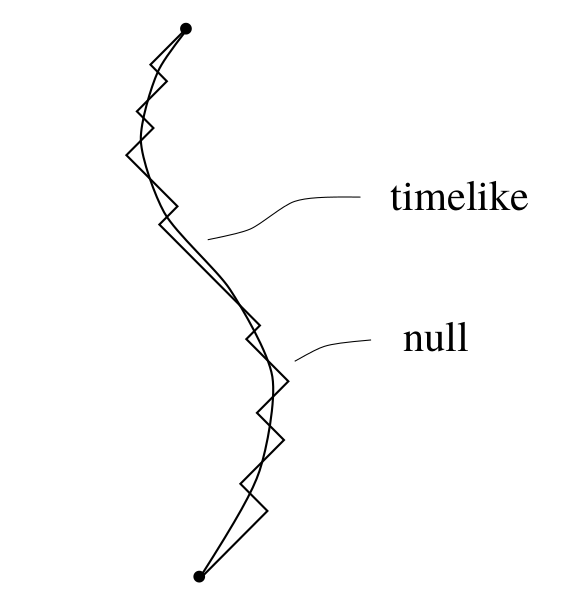
\includegraphics[width=0.7\linewidth]{gfx/ApproximateTimelikeByNullGeodesic}
	\caption{}
	\label{fig:approximatetimelikebynullgeodesic}
\end{figure}
consider “jagged” null curves which follow the timelike one: \\
\todo{I dont understand this argument, shouldnt it be exactly the other way around. I.e. since it is infinitesimally approximated by zero proper time, shouldnt it be minimum proper time ?}
As we increase the number of sharp corners, the null curve comes closer and closer to the
timelike curve while still having zero path length. Timelike geodesics cannot therefore be
curves of minimum proper time, since they are always infinitesimally close to curves of zero
proper time; in fact they maximize the proper time. (This is how you can remember which
twin in the twin paradox ages more — the one who stays home is basically on a geodesic,
and therefore experiences more proper time.)\\
Of course even this is being a little cavalier;
actually every time we say “maximize” or “minimize” we should add the modifier “locally.”
It is often the case that between two points on a manifold there is more than one geodesic.
For instance, on S 2 we can draw a great circle through any two points, and imagine travelling
between them either the short way or the long way around. One of these is obviously longer
than the other, although both are stationary points of the length functional.















\section{An equivalent consideration of parallel transport, geodesics}
Having set up the machinery of connections as exemplified by \ref{fig:flowmanifoldstructure}, the first thing we will do is discuss parallel
transport. Recall that in flat space it was unnecessary to be very careful about the fact
that vectors were elements of tangent spaces defined at individual points; it is actually very
natural to compare vectors at different points (where by “compare” we mean add, subtract,
take the dot product, etc.). The reason why it is natural is because it makes sense, in flat
space, to “move a vector from one point to another while keeping it constant.” Then once
we get the vector from one point to another we can do the usual operations allowed in a
vector space. The concept of moving a vector along a path, keeping constant all the while, is known
as \emph{parallel transport}. As we shall see, parallel transport is defined whenever we have a connection; the intuitive manipulation of vectors in flat space makes implicit use of the
Christoffel connection on this space. The crucial difference between flat and curved spaces is
that, in a curved space, \emph{the result of parallel transporting a vector from one point to another
	will depend on the path taken between the points}.\\
\\
Without yet assembling the complete
mechanism of parallel transport, we can use our intuition about the two-sphere to see that
this is the case. Start with a vector on the equator, pointing along a line of constant
longitude. Parallel transport it up to the north pole along a line of longitude in the obvious
way. Then take the original vector, parallel transport it along the equator by an angle $θ$, and
then move it up to the north pole as before. It is clear that the vector, parallel transported
along two paths, arrived at the same destination with two different values (rotated by $θ$).
\begin{figure}[h!]
	\centering
	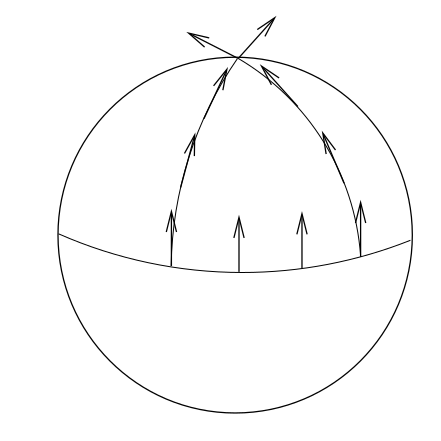
\includegraphics[width=0.7\linewidth]{gfx/ParalleltransportTwosphere}
	\caption{}
	\label{fig:paralleltransporttwosphere}
\end{figure}

It therefore appears as if there is no natural way to uniquely move a vector from one
tangent space to another; we can always parallel transport it, but the result depends on the
path, and there is no natural choice of which path to take. Unlike some of the problems we
have encountered, there is no solution to this one — we simply must learn to live with the
fact that two vectors can only be compared in a natural way if they are elements of the same
tangent space. For example, two particles passing by each other have a well-defined relative
velocity (which cannot be greater than the speed of light). But two particles at different
points on a curved manifold do not have any well-defined notion of relative velocity — the
concept simply makes no sense.\\
In cosmology, for example, the light from distant galaxies
is redshifted with respect to the frequencies we would observe from a nearby stationary
source. Since this phenomenon bears such a close resemblance to the conventional Doppler
effect due to relative motion, it is very tempting to say that the galaxies are “receding away
from us” at a speed defined by their redshift. At a rigorous level this is nonsense, what
Wittgenstein would call a “grammatical mistake” — the galaxies are not receding, since the
notion of their velocity with respect to us is not well-defined. What is actually happening
is that the metric of spacetime between us and the galaxies has changed (the universe has expanded) along the path of the photon from here to there, leading to an increase in the
wavelength of the light. As an example of how you can go wrong, naive application of the
Doppler formula to the redshift of galaxies implies that some of them are receding faster than
light, in apparent contradiction with relativity. The resolution of this apparent paradox is
simply that the very notion of their recession should not be taken literally.
\\
\\
The notion of parallel transport is obviously dependent on the connection, and different
connections lead to different answers. If the connection is metric-compatible, the metric is
always parallel transported with respect to it
\begin{equation}
	\nabla_{\dot{\gamma}} g_{\mu \nu} = \frac{\md x^\sigma}{\md \lambda} \nabla_\sigma g_{\mu \nu} =0.
\end{equation}
It follows that the inner product of two parallel-transported vectors is preserved. This means that parallel transport with respect to a metric-compatible connection preserves
the norm of vectors, the sense of orthogonality.

\subsection{Formal solution to the parallel transport equation}
You can write down an explicit
and general solution to the parallel transport equation, which reads for a tensor
\begin{equation}
	\frac{\md x^\sigma}{\md \lambda} \nabla_\sigma T^{\mu_1 \dots \mu_k}_{\qquad \quad \nu_1 \dots \nu_l}=0
\end{equation}
or for a vector
\begin{equation}
	\frac{\md }{\md \lambda} V^\mu + \Gamma^\mu_{\sigma \rho} \frac{\md x^\sigma}{\md \lambda} V^\rho = 0,
\end{equation}

 although it’s somewhat formal. First
notice that for some path $γ : λ → x^σ (λ)$, solving the parallel transport equation for a vector
$V^\mu$ amounts to finding a matrix $P^μ_ρ (λ, λ_0 )$ which relates the vector at its initial value $V^μ (λ_0 )$
to its value somewhere later down the path:
\begin{equation}
	V^\mu (\lambda) = P^\mu_{\rho}(\lambda, \lambda_0) V^\rho (\lambda_0).
\end{equation}
Of course the matrix $P^μ_ρ (λ, λ_0 )$, known as the \emph{parallel propagator}, depends on the path
$γ$ (although it’s hard to find a notation which indicates this without making γ look like an
index). If we define
\begin{equation}
	A^\mu_\rho (\lambda) = -  \Gamma^\mu_{\rho \sigma} \frac{\md x^\sigma}{\md \lambda},
\end{equation}
where the quantities on the RHS are evaluated at $x^\nu(\lambda)$, then the parallel transport
equation becomes
\begin{equation}
	\frac{\md}{\md \lambda} V^\mu (\lambda) = A^\mu_\rho V^\rho.
\end{equation}
Since the parallel propagator must work for any vector, substituting it in shows
that $P^μ_ρ (λ, λ_0 )$ also obeys this equation:
\begin{equation}
	\frac{\md}{\md \lambda} P^\mu_\rho (\lambda, \lambda_0)= A^\mu_\sigma(\lambda) P^\sigma_\rho(\lambda,\lambda_0).
\end{equation}
To solve this equation, first integrate both sides:
\begin{equation}
P^\mu_\rho (\lambda,\lambda_0) = \delta^\mu_\nu + \int_{\lambda_0}^{\lambda} A^\mu_\sigma (\eta) P^\sigma_\rho(\eta, \lambda_0) \md \eta.
\end{equation}
The Kronecker delta, it is easy to see, provides the correct normalization for $λ = λ_0$ .
We can solve this by iteration, taking the right hand side and plugging it into itself
repeatedly, giving
\begin{equation}
	P^\mu_\rho(\lambda,\lambda_0) = \delta^\mu_\rho + \int_{\lambda_0}^{\lambda} A^\mu_\rho (\eta) \md \eta + \int_{\lambda_0}^\lambda  \int_{\lambda_0}^\eta A^\mu_\sigma(\eta) A^\sigma_\rho (\eta^\prime) \md \eta^\prime \md \eta + \dots 
\end{equation}
The $n$th term in this series is an integral over an $n$-dimensional right triangle, or n-simplex.


\begin{figure}[h!]
	\centering
	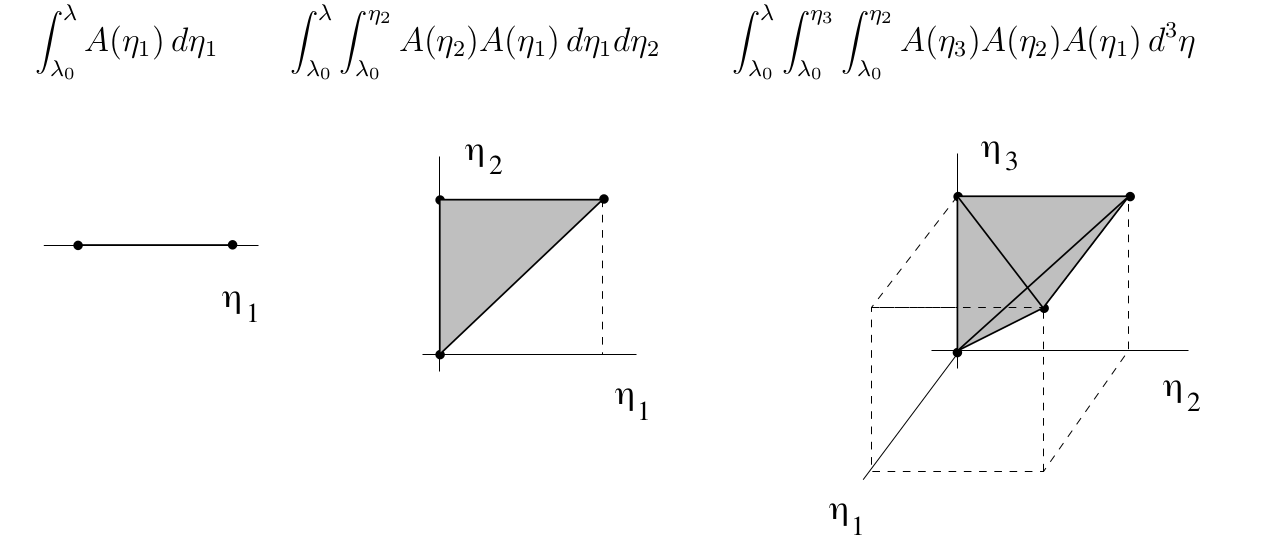
\includegraphics[width=0.7\linewidth]{gfx/SolutionGeodesicEquation}
	\caption{}
	\label{fig:solutiongeodesicequation}
\end{figure}

It would simplify things if we could consider such an integral to be over an $n$-cube
instead of an $n$-simplex; is there some way to do this? There are $n!$ such simplices in each
cube, so we would have to multiply by $1/n!$ to compensate for this extra volume. But we
also want to get the integrand right; using matrix notation, the integrand at $n$th order
is $A(η_n )A(η_{n−1} ) · · · A(η_1 )$, but with the special property that $η_n ≥ η_{n−1} ≥ · · · ≥ η_1$ . We
therefore define the \emph{path-ordering symbol} $\mathcal{P}$ to ensure that this condition holds. In
other words, the expression
\begin{equation}
	\mathcal{P}\left[A(\eta_n) \dots A(\eta_1)\right]
\end{equation}
Stands for the product of the $n$ matrices $A(η_i )$, ordered in such a way that the largest value
of $η_i$ is on the left, and each subsequent value of $η_i$ is less than or equal to the previous one.
We then can express the $n$th-order term in the solution as
\begin{equation}
	\int_{\lambda_0}^\lambda \int_{\lambda_0}^{\eta_n} \dots \int_{\lambda_0}^{\eta_2} A(\eta_n) \dots A(\eta_1) \md^n \eta = \frac{1}{n!}\int_{\lambda_0}^\lambda \int_{\lambda_0}^\lambda \dots \int_{\lambda_0}^\lambda \mathcal{P}\left[A(\eta_n) \dots A(\eta_1)\right] \md^n \eta.
\end{equation}
This yields the solution to the parallel propagator as
\begin{equation}
	P(\lambda,\lambda_0) = \mathcal{I} + \sum_{i=n}^{\infty} \frac{1}{n!} \int_{\lambda_0}^\lambda  \mathcal{P}\left[A(\eta_n) \dots A(\eta_1)\right] \md^n \eta = \mathcal{P} \exp\left(\int_{\lambda_0}^\lambda A(\eta) \md \eta\right).
\end{equation}
Or more explicitly
\begin{equation}
	P^\mu\nu (\lambda, \lambda_0) = \mathcal{P} \exp \left(-\int_{\lambda_0}^\lambda \Gamma^\mu_{\sigma \nu} \frac{\md x^\sigma}{\md \eta}  \md \eta\right).
\end{equation}
The same kind of expression appears in quantum field theory as “Dyson’s Formula,” where it arises because the
Schrödinger equation for the time-evolution operator has the same form as this.\\
\\
As an aside, an especially interesting example of the parallel propagator occurs when the
path is a loop, starting and ending at the same point. Then if the connection is metric-
compatible, the resulting matrix will just be a Lorentz transformation on the tangent space
at the point. This transformation is known as the “holonomy” of the loop. If you know
the holonomy of every possible loop, that turns out to be equivalent to knowing the metric.




\section{Curvature}

The invariant quantities which characterize the geometry in a way which is independent of particular choice of coordinates are curvatures. The curvatures are precisely a measure of the local mismatch between the surface and the tangent plane. Since the tangent space is flat, the derivatives of the components contain no terms due to the curving of the coordinates, and the gradients of vectors w.r.t. flat coordinates are tensors.\\
\\
To compute the covariant derivative of a tensor having many indices the rules is that each index brings an added term involving $\Gamma$ and the tensor itself. Indices can be up or down only in one way and it is only the identification $+$ with up, $-$ with down that needs to be memorized
\\
The fact that the curvature tensor appears as  connecting the second covariant derivatives 
\begin{equation}
A^\mu_{; \sigma \tau} - A^\mu_{;\tau \sigma} = \bar{R}^\mu_{\rho \sigma \tau} A^\rho
\end{equation}
serves as a clue that enables us to give another useful geometrical picture of curvature. The noncommuting property of the second derivatives represents a limit of differences in the vector as we move first a displacement along axis $\sigma$ and then along $\tau$, or first along $\tau$  and the along $\sigma$. If the coordinates are flat, for a constant vector there is no difference. If we have curved space as we take these displacements in different orders, we find different resulting vectors. The curvature $K$ of a surface is defined in terms of the angle through which a vector is turned as we take it around an infinitesimal closed path. The generalized definition of curvature of a many-dimension surface will be given i.t.o. the change in a vector as it is carried about a closed path, keeping it parallel to itself. Since the orientation of a path lying on a definite plane depends on two coordinate axes, we see that the curvature will have the general character of a fourth rank tensor.

\subsection{Torsion and metric connection}
\begin{mybox}{Torsion}
	The torsion $T$ maps two vector field $x$ and $y$ into another vector field 
	\begin{equation}
		T:TM \times TM \rightarrow TM, (x,y) \mapsto T(x,y) = \nabla_x y - \nabla_y x - [x,y],
	\end{equation}
	where the commutator of two vector fields is defined as $[X,Y]^\mu= X^\lambda \partial_\lambda Y^\mu - Y^\lambda \partial_\lambda X^\mu$.
	In components
	\begin{equation}
		T^i_{jk} = \Gamma^i_{jk} - \Gamma^i_{kj}.
	\end{equation}
	The torsion vanishes if and only if the connection is symmetric, i.e. if the Christoffel's are symmetric. The torsion
	quantifies whether parallelograms spanned by two vectors close
\end{mybox}
On a manifold $(M,g)$, a symmetric connection can always be uniquely defined by requiring that $\nabla g=0, \nabla_{\sigma} g_{\mu \nu} =0, \nabla_{\sigma} g^{\mu \nu}=0$. This is the \emph{Levi-Civita, or Riemannian} connection, whose Christoffel symbols are
\begin{equation}
	\Gamma^i_{jk} = \half g^{ia} \left(\partial_j g_{ak} + \partial_k g_{j a}\ - \partial_a g_{jk} \right).
\end{equation}
From now on, we shall assume that we are working with a Levi-Civita connectin whose torsion vanishes.



\subsection{How to get from the connection coefficients to the connection-the metric connection}


To define a covariant derivative, then, we need to put a “connection” on our manifold,
which is specified in some coordinate system by a set of coefficients $Γ^\lambda_{\mu \nu}$ ($n^3 = 64$ independent
components in $n = 4$ dimensions) which transform according to \ref{eq:christoffelTrafo}. (The name “connection” comes from the fact that it is used to transport vectors from one tangent space to
another.) There are evidently a large number of connections we could
define on any manifold, and each of them implies a distinct notion of covariant differentiation. In general relativity this freedom is not a big concern, because it turns out that every
metric defines a unique connection, which is the one used in GR. Let’s see how that works.\\
\\
The first thing to notice is that the difference of two connections is a $(1, 2)$ tensor. If
we have two sets of connection coefficients,$ Γ^{\lambda}_{μν}$ and $\hat{\Gamma}^\lambda_{\mu \nu}$, their difference $S^{\quad \lambda}_{\mu \nu} = \Gamma^\lambda_{\mu \nu} - \hat{\Gamma}^\lambda_{\mu \nu}$ (notice index placement, here it matters since it is a tensor) transforms as
\begin{equation}
S^{\quad \lambda^\prime}_{\mu^\prime \nu^\prime} =..= \frac{\partial x^\mu}{\partial x^{\mu^\prime}} \frac{\partial x^\nu}{\partial x^{\nu^\prime}} \frac{\partial x^{\lambda^\prime}}{\partial x^\lambda} S^{\quad \lambda}_{\mu \nu}
\end{equation}
This is just the tensor transformation law, so $S^\lambda_{\mu \nu}$ is indeed a tensor. This implies that any
set of connections can be expressed as some fiducial connection plus a tensorial correction.
Next notice that, given a connection specified by $Γ^λ_{μν}$ , we can immediately form another
connection simply by permuting the lower indices. That is, the set of coefficients $Γ^λ_{νμ}$ will
also transform according to \ref{eq:christoffelTrafo} (since the partial derivatives appearing in the last term
can be commuted), so they determine a distinct connection. There is thus a tensor we can
associate with any given connection, known as the \emph{torsion tensor}, defined by
\begin{equation}
	T^{\quad \lambda}_{\mu \nu} = \Gamma^\lambda_{\mu \nu} - \Gamma^\lambda_{\nu \mu} = 2 \Gamma^\lambda_{[\mu nu]}.
\end{equation}
It is clear that the torsion is antisymmetric its lower indices, and a connection which is
symmetric in its lower indices is known as “torsion-free.”\\
We can now define a unique connection on a manifold with a metric $g_{μν}$ by introducing
two additional properties:
\begin{enumerate}
\item  torsion-free: $Γ^λ_{μν} = Γ^λ_{ (μν)}$ .
\item Metric compatibility: $\nabla_\rho g_{\mu \nu} =0.$
\end{enumerate}
A connection is \emph{metric compatible} if the covariant derivative of the metric with respect to
that connection is everywhere zero. This implies a couple of nice properties. First, it’s easy
to show that the inverse metric also has zero covariant derivative,
\begin{equation}
	\nabla_\rho g^{\mu \nu} = 0.
\end{equation}
Second, a metric-compatible covariant derivative commutes with raising and lowering of
indices.\\
Our claim is therefore that there is exactly one torsion-free connection on a given manifold
which is compatible with some given metric on that manifold. We do not want to make these
two requirements part of the definition of a covariant derivative; they simply single out one
of the many possible ones. We can demonstrate both existence and uniqueness by deriving a manifestly unique
expression for the connection coefficients in terms of the metric. To accomplish this, we
expand out the equation of metric compatibility for three different permutations of the
indices:
\begin{equation}
	\nabla_\rho g_{\mu \nu} = \partial_\rho - \Gamma^\lambda_{\rho \mu} g_{\lambda \nu} - \Gamma^\lambda_{\rho \nu} g_{\lambda \mu}, \quad \nabla_\nu g_{\rho \mu} = ....
\end{equation}
Manipulating these equations yields the unique form of the Christoffel symbols for the metric connection
\begin{equation}
\label{eq:Christoffels}
	\Gamma^\sigma_{\mu \nu} = \frac{1}{2} g^{\sigma \rho} \left[\partial_{\mu} g_{\nu \rho} + \partial_\nu g_{\rho \mu} - \partial_\rho g_{\mu \nu} \right].
\end{equation}
This is one of the most important formulas in this subject; commit it to memory. Of course,
we have only proved that if a metric-compatible and torsion-free connection exists, it must
be of the form \ref{eq:Christoffels}; you can check for yourself (for those of you without enough tedious
computation in your lives) that the right hand side of \ref{eq:Christoffels} transforms like a connection.
This connection we have derived from the metric is the one on which conventional general
relativity is based (although we will keep an open mind for a while longer). It is known
by different names: sometimes the \emph{Christoffel connection}, sometimes the \emph{Levi-Civita
connection}, sometimes the \emph{Riemannian connection}. The associated
connection coefficients are sometimes called Christoffel symbols. The study of manifolds with
metrics and their associated connections is called “Riemannian geometry.”\\
\\
Let’s emphasize again that the connection does \emph{not have to be} constructed
from the metric. In ordinary flat space there is an implicit connection we use all the time
— the Christoffel connection constructed from the flat metric. But we could, if we chose,
use a different connection, while keeping the metric flat. Also notice that the coefficients
of the Christoffel connection in flat space will vanish in Cartesian coordinates, but not in
curvilinear coordinate systems. The existence of nonvanishing connection coefficients in curvilinear coordinate systems is
the ultimate cause of the formulas for the divergence and so on that you find in books on
electricity and magnetism.

\subsection{Conceptional flow of how to add structure on our mathematical constructs}
Before moving on, let’s review the process by which we have been adding structures to
our mathematical constructs. We started with the basic notion of a set, which you were
presumed to know (informally, if not rigorously). We introduced the concept of open subsets
of our set; this is equivalent to introducing a topology, and promoted the set to a topological
space. Then by demanding that each open set look like a region of $\mR^n$ (with $n$ the same for
each set) and that the coordinate charts be smoothly sewn together, the topological space
became a manifold. A manifold is simultaneously a very flexible and powerful structure,
and comes equipped naturally with a tangent bundle, tensor bundles of various ranks, the
ability to take exterior derivatives, and so forth. We then proceeded to put a metric on
the manifold, resulting in a manifold with metric (or sometimes “Riemannian manifold”).
Independently of the metric we found we could introduce a connection, allowing us to take
covariant derivatives. Once we have a metric, however, there is automatically a unique
torsion-free metric-compatible connection. (In principle there is nothing to stop us from
introducing more than one connection, or more than one metric, on any given manifold.)
\begin{figure}[h!]
	\centering
	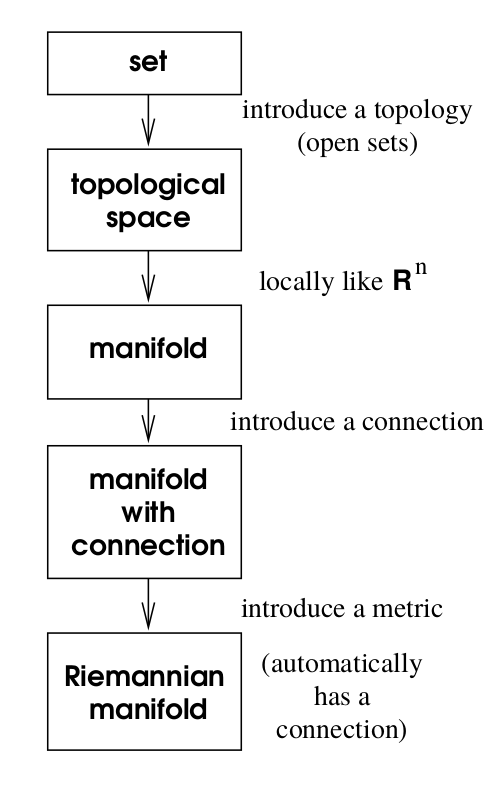
\includegraphics[width=0.7\linewidth]{gfx/FlowManifoldStructure}
	\caption{}
	\label{fig:flowmanifoldstructure}
\end{figure}

\subsection{The curvature}
The idea behind this measure of curvature, the Riemann tensor which is derived from the connection, is that we
know what we mean by “flatness” of a connection — the conventional (and usually implicit)
Christoffel connection associated with a Euclidean or Minkowskian metric has a number of
properties which can be thought of as different manifestations of flatness. These include the
fact that parallel transport around a closed loop leaves a vector unchanged, that covariant
derivatives of tensors commute, and that initially parallel geodesics remain parallel. It would be more useful to have a local description of the curvature at each point, which is what the Riemann tensor is supposed to provide. One conventional way to introduce the
Riemann tensor, therefore, is to consider parallel transport around an infinitesimal loop.\\
We want to construct a tensor out of the metric and its derivatives. If we use only $g\munu$ and its first derivatives, then no new tensor can be constructed, for at any point we can find a coordinate system (RNC) in which the first deriavtives of the metric tensor vanish, so in this coordinate system the desired tensor must be equal to one of those that can be constructed out of the metric tensor \emph{alone}, and since this is an equality between tensors it must be true in all coordinate systems. Hence our search for this tensor is motivated by the Principle of General Covariance.
\begin{mybox}{Curvature and Curvature tensor}
	The curvature $\bar{R}$ maps three vector field $x,y$ and $v$ into a vector field,
	\begin{align}
		\bar{R}:TM\times TM \times TM &\rightarrow TM,\\
		 (x,y,z) \mapsto \bar{R}(x,y) v &= \nabla_x(\nabla_y v) - \nabla_y(\nabla_x v) \nabla_{[x,y]} v.
	\end{align} 
Note that the two vectors $x$ and $y$ appearing here correspond
to the two antisymmetric indices in the component form of the Riemann tensor. The last
term, involving the commutator $[x, y ]$, vanishes when $x$ and $y$ are taken to be
the coordinate basis vector fields (since $[∂_μ , ∂_ν ] = 0$), which is why this term did not arise
when we take the commutator of two covariant derivatives as performed below.\\
Since the covariant derivatives $\nabla_x$ and $\nabla_y$ represent the infinitesimal parallel transports along the integral curves of the vector fields $x$ and $y$, the curvature $\bar{R}$ directly quantifies the change of the vector $v$ when it is parallel-transported around an infinitesimal, closed loop.
\\
The \emph{curvature or Riemann tensor} $\bar{R} \in \mathcal{T}^1_3$ is given by 
\begin{equation}
\bar{R}:T^*M\times TM \times TM \times TM \rightarrow \mR, (w,x,y,z) \mapsto w[\bar{R}(x,y)z].
\end{equation}
Its components are 
\begin{align}
\bar{R}^i_{\; j k l} &= \md x^i [\bar{R}(\partial_k, \partial_l) \partial_j] \\
							&= \partial_k \Gamma^i_{jl} - \partial_l \Gamma^i_{jk} + \Gamma^a_{jl} \Gamma^i_{ak} - \Gamma^a_{jk} \Gamma^i_{al}.
\end{align}
The Riemann tensor is antisymmetric, i.e. $i=j => \bar{R}=0$ and obeys $3$ further symmetries 
\begin{align}
	\bar{R}_{ijkl} &= -\bar{R}_{jikl} =\bar{R}_{jilk} \\
	\bar{R}_{ijkl} &= \bar{R}_{klij}
\end{align}
such that it only has $21$ independent components.\\
All of the components of $\bar{R}^{\sigma}_{\mu \alpha \beta}$ vanish if and only if the space is flat. Operationally, "flat" means that there exists a global coordinate system in which the metric components are everywhere constant.
\end{mybox}
One can equivalently find the form of the Riemann tensor by considering a related operation, the commutator of two covariant derivatives. The relationship between this and parallel transport around a loop should be evident;
the covariant derivative of a tensor in a certain direction measures how much the tensor
changes relative to what it would have been if it had been parallel transported (since the
covariant derivative of a tensor in a direction along which it is parallel transported is zero).
The commutator of two covariant derivatives, then, measures the difference between parallel
transporting the tensor first one way and then the other, versus the opposite ordering.
\begin{equation}
	[\nabla_\mu, \nabla_\nu] V^\rho = ..= \underbrace{\left(\partial_\mu \Gamma^\rho_{\nu \sigma} - \partial_\nu \Gamma^\rho_{\mu \sigma} + \Gamma^\rho_{\mu \lambda}\Gamma^\lambda_{\nu \sigma} -\Gamma^\rho_{\nu \lambda}\Gamma^\lambda_{\mu \sigma} \right)}_{\bar{R}^\rho_{\sigma \mu \nu}} V^\sigma - \underbrace{2 \Gamma^\lambda_{[\mu \nu]}}_{T^{\,\, \lambda}_{\mu\nu}} \nabla_\lambda V^\rho.
\end{equation}
Note:\\
The Riemann tensor measures that part of
the commutator of covariant derivatives which is proportional to the vector field, while
the torsion tensor measures the part which is proportional to the covariant derivative
of the vector field; the second derivative doesn’t enter at all.\\
\\
Having defined the curvature tensor as something which characterizes the connection, let
us now admit that in GR we are most concerned with the Christoffel connection. In this
case the connection is derived from the metric, and the associated curvature may be thought
of as that of the metric itself. This identification allows us to finally make sense of our
informal notion that spaces for which the metric looks Euclidean or Minkowskian are flat.
In fact it works both ways: if the components of the metric are constant in some coordinate
system, the Riemann tensor will vanish, while if the Riemann tensor vanishes we can always
construct a coordinate system in which the metric components are constant\\
\\
\subsection{Independent components of the Riemann tensor and intuition for curvature}
Given these relationships between the different components of the Riemann tensor, how
many independent quantities remain? Let’s begin with the facts that $\bar{R}_{ρσμν}$ is antisymmetric
in the first two indices, antisymmetric in the last two indices, and symmetric under interchange of these two pairs. This means that we can think of it as a symmetric matrix $\bar{R}_{[ρσ][μν]}$ ,
where the pairs $ρσ$ and $μν$ are thought of as individual indices. An $ m × m$ symmetric matrix has $m(m + 1)/2$ independent components, while an $n × n$ antisymmetric matrix has
$n(n − 1)/2$ independent components. We therefore have
\begin{equation}
	\half \left[\half n(n-1)\right]\left[\half n(n-1) +1\right] = \frac{1}{8} \left(n^4-2n^3+3n^2- 2n\right)
\end{equation}
independent components. The first Bianchi identity implies together with the antisymmetry of the Riemann tensor that $\bar{R}_{[\rho\sigma\mu\nu]}=0$.
Now a totally antisymmetric $4$-index tensor has $n(n−1)(n−2)(n−3)/4!$ terms, and therefore we are left with
\begin{equation}
\label{eq:dofRiemann}
	 \frac{1}{8} \left(n^4-2n^3+3n^2- 2n\right)-n(n−1)(n−2)(n−3)/4! = \frac{1}{12} n^2 (n^2-1)
\end{equation}
independent components, i.e. $20$ for $n=4$ spacetime dimensions.\\
\\\marginpar{ A curvature radius is only appropriate for "extrinsic" curvature – the curvature of a line/submanifold embedded into a higher-dimensional space. The Riemann tensor measures all the components of the intrinsic curvature so they're not exactly the same. }
After this large amount of formalism, it might be time to step back and think about what
curvature means for some simple examples. First notice that, according to \ref{eq:dofRiemann}, in $1, 2, 3$
and $4$ dimensions there are $0, 1, 6$ and $20$ components of the curvature tensor, respectively.
(Everything we say about the curvature in these examples refers to the curvature associated
with the Christoffel connection, and therefore the metric.) This means that one-dimensional
manifolds (such as $S^1$, i.e. a circle ) are never curved; the intuition you have that tells you that a circle is
curved comes from thinking of it embedded in a certain flat two-dimensional plane. (There is
something called “extrinsic curvature,” which characterizes the way something is embedded
in a higher dimensional space. Our notion of curvature is “intrinsic,” and has nothing to do
with such embeddings.)\\
The distinction between intrinsic and extrinsic curvature is also important in two dimensions, where the curvature has one independent component. (In fact, all of the information about the curvature is contained in the single component of the Ricci scalar.)\\
Consider a
cylinder, $\mR × S^1$ . Although this looks curved from our point of view, it should be clear
that we can put a metric on the cylinder whose components are constant in an appropriate
coordinate system — simply unroll it and use the induced metric from the plane. In this
metric, the cylinder is flat. (There is also nothing to stop us from introducing a different
metric in which the cylinder is not flat, but the point we are trying to emphasize is that it
can be made flat in some metric.)
\begin{figure}[h!]
	\centering
	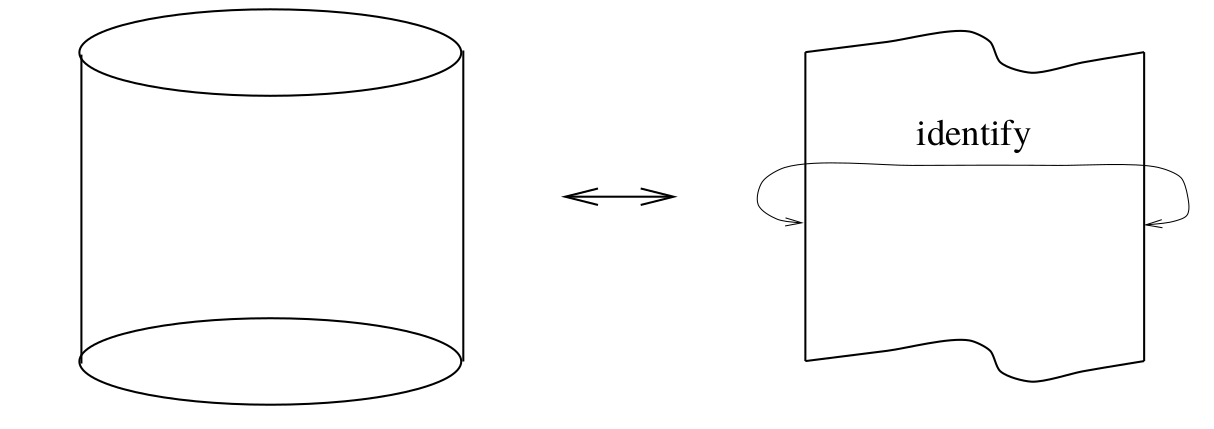
\includegraphics[width=0.7\linewidth]{gfx/CurvatureCylinder}
	\caption{\itshape I.e. cylinder is not curved since it can be glued together by flat spaces.}
	\label{fig:curvaturecylinder}
\end{figure}
Positively curved spaces have a positively curved Ricci scalar, whereas flat spaces have a vanishing one etc.


\subsubsection{Uniqueness by General Covariance ? Weinberg}
The existence of the tensor $\bar{R}^\rho_{\mu \lambda \nu}$ raises the question of whether or not the Principle of Equivalence or the Principle of General Covariance uniquely determines the effects of gravitation on arbitrary physical systems. For instance, let us ask whether the correct e.o.m. for a freely falling particle of spin $S_\mu$ might be of the form
\begin{equation}
	0 = \frac{\md^2 x^\lambda}{\md \tau^2} + \Gamma^\lambda_{\mu \nu} \frac{\md x^\mu}{\md \tau} \frac{\md x^\nu}{\md \tau} + f R^\lambda_{\mu \nu \kappa} \frac{\md x^\mu}{\md \tau} \frac{\md x^\nu}{\md \tau} S^\kappa
\end{equation}
(with $f$ and unknown scalar) instead of the familiar geodesic equation \ref{eq:geodesicequation}. Both equations are generally covariant, and both reduce in the absence of gravitation to be correct special-relativistic equation $\md U^\alpha /\md \tau =0$. How then can we tell whether one or the other is correct ?\\
The answer is one of \emph{scale}. Suppose that our particle has a characteristic linear dimension $d$, and that the gravitational field has a characteristic space-time dimension $D$. The Riemann tensor has one more derivative of the metric than the affine connection coefficients, so the ratio of the third term in the first equation to the second term is proportional to $1/D$; dimensional considerations then require that this ratio be roughly of order $d/D$. Thus, barring special circumstances that might make one term or the other anomalously large or small, we can regard the last term in the first equation as being negligible if our particle is very much smaller than the characteristic dimensions of the gravitational field, and the geodesic equation is the correct e.o.m. Of course, if our particle is not much smaller than the gravitational field scale (as in the case of the moon moving in the gravitational field of the earth), then the Principle of Equivalence or the Principle of General Covariance must be applied to the infinitesimal elements of which the particle is composed, although both equations might give a fair phenomenological representation of the motion of the whole particle.\\
\\
Note further that one can prove that the Riemann tensor is the \emph{only} tensor that can be constructed from the metric tensor and its first and second derivatives, and is linear in the second derivatives.






\subsection{The Ricci tensor}
The symmetry in the first and last index pair of the Riemann tensor shows that the Ricci tensor is symmetric. Furthermore, the antisymmetry of the Riemann tensor in the first and last index pair tells us that the Ricci tensor is essentially the only second-rank tensor that can be formed from the Riemann tensor, since
multiplying the antisymmetry condition of the Riemann tensor with $g^{\lambda \nu}$, $g^{\lambda \mu}$, and $g^{\nu \kappa}$ gives
\begin{equation}
	R_{\mu \kappa} = -g^{\lambda \nu} \bar{R}_{\mu \lambda \nu \kappa} = - g^{\lambda \nu} \bar{R}_{\lambda \mu \kappa \nu} = + g^{\lambda \nu} \bar{R}_{\mu\lambda \kappa \nu}
\end{equation}
and 
\begin{equation}
	g^{\lambda \mu} \bar{R}_{\lambda \mu \nu \kappa} = g^{\nu \kappa} \bar{R}_{\lambda \mu \nu \kappa}=0.
\end{equation}
From the antisymmetry property of the Riemann tensor we also see that there is essentially only one way of contracting the Riemann tensor to construct a scalar:
\begin{equation}
	\mathcal{R}=g^{\lambda \nu} g^{\mu \kappa} \bar{R}_{\lambda \mu \nu \kappa} = - g^{\lambda \nu} g^{\mu \kappa} \bar{R}_{\mu \lambda \nu \kappa}, \; 0 = g^{\lambda \mu} g^{\nu \kappa} \bar{R}_{\lambda \mu \nu \kappa}.
\end{equation}
\begin{mybox}{Ricci tensor}
	The symmetric \emph{Ricci tensor} $R$ is the contraction $C^1_3 \bar{R}$ of the curvature tensor $\bar{R}$. Its components are 
	\begin{equation}
		R_{jl} = \bar{R}^i_{jil} = g^{i m} \bar{R}_{mjil}=\partial_i \Gamma^i_{lj} - \partial_l \Gamma^i_{ij} + \Gamma^m_{lj} \Gamma^i_{im} - \Gamma^m_{ij} \Gamma^i_{lm}.
	\end{equation}
	For a symmetric connection with a vanishing torsion, the \emph{Bianchi identity} 
	\begin{equation}
	\nabla_{[\lambda} \bar{R}_{\rho \sigma] \mu \nu} =0
	\end{equation}
	reduces to 
	\begin{align}
	\bar{R}_{\rho \sigma \mu \nu} + \bar{R}_{\rho \mu \nu \sigma}+\bar{R}_{\rho \nu \sigma \mu} & = 0,\\
	 				\nabla_\lambda \bar{R}_{\rho \sigma \mu \nu}+\nabla_\rho \bar{R}_{\sigma \lambda \mu \nu}+\nabla_\sigma\bar{R}_{\lambda \rho \mu \nu} &=0.
	\end{align}
	The contracted Ricci tensor yields the \emph{Ricci scalar}
	\begin{equation}
	 \mathcal{R} = R^i_i = tr(R).
	\end{equation}
	The \emph{contracted Bianchi identitiy} then reads
	\begin{equation}
		\left[R^i_j -\frac{\mathcal{R}}{2} \delta^i_j\right]_{;i} = 0.
	\end{equation}
	One then has the relation
	\begin{align}
		\bar{R}_{\lambda \mu \nu \kappa} &= g_{\lambda \nu} R_{\mu \kappa} - g_{\lambda \kappa} R_{\mu \nu} - g\munu R_{\lambda \kappa} + g_{\mu \kappa} R_{\lambda \nu} \nonumber \\
		&- \half \left[g_{\lambda\nu} g_{\mu \kappa} - g_{\lambda\kappa} g\munu\right] \mathcal{R}.
	\end{align}
\end{mybox}
\subsection{The Einstein tensor}
The symmetric \emph{Einstein tensor} is given by
\begin{equation}
G_{ij} = R_{ij}  -\frac{\mathcal{R}}{2} g_{ij},
\end{equation}
which has vanishing divergence by the twice contracted Bianchi identity $\nabla^{\mu} G_{\mu \nu} = 0$ $\leftrightarrow$ $G^i_{jji} =0$.
The Einstein tensor is symmetric due to the symmetry of the Ricci tensor and the
metric.


















\section{The Lie derivative}
Another important tensorial derivative is the \emph{Lie derivative}, which is independent of the metric. Whereas the covariant derivative required an affine connection to allow comparison between vectors at different points, the Lie derivative uses a congruence from a vector field to achieve the same purpose. In GR, a congruence is the set of integral curves of a vector field in a $4-d$ manifold.\\
The idea of Lie dragging a function along a congruence leads to the definition of the Lie derivative, wehre the dragged function is compared with the value of the original function at a given point. It is defined as 
\begin{equation}
\mathcal{L}_x :\mathcal{T}^r_s \rightarrow \mathcal{T}^r_s,
\end{equation}
where $x$ is the vector field along whose congruence the Lie derivative is taken.\\
The Lie derivative of a scalar is just the directional derivative.\\
\\
\subsection{Pull-back and Push-forward}
A differentiable curve $\gamma_t(p)$ defined at every point $p \in M$ defines a diffeomorphic map $\phi_t:M\rightarrow M$. If $\dot{\gamma}_t=v$ for a vector field $v \in TM$, $\phi_t$ is called the \emph{flow} of $v$ .If a tangent vector defined by 
\begin{equation}
	(\dot{\gamma}(t))(f) = \frac{\md }{\md t} (f \circ \gamma) (t)
\end{equation}
suffices $\dot{\gamma}=v$, then $\gamma$ is called an \emph{integral curve} of $v$. Equivalently, given a coordinate system $x^μ$ on
M , the components of $\dot{\gamma}$ in that coordinate system must satisfy
\begin{equation}
	\dot{\gamma}^\mu = \frac{\md}{\md t} x^\mu (\gamma(t)),
\end{equation}
where $t$ parametrizes the curve $\gamma$, could also choose $\lambda$ etc.\\

If this is true for all curves $\gamma$ obtained from $\gamma_t$ by specifying $\gamma(0)$, the result is called flow of v.
\begin{figure}[h!]
	\centering
	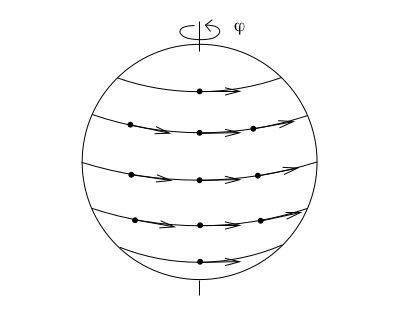
\includegraphics[width=0.7\linewidth]{gfx/IntegralCurvesTwoSphere}
	\caption{\itshape E.g. integral curves on the two-sphere, defining the rotations by a given angle. The tangent vectors infinitesimmaly generate the rotation. Compare treatment in \ref{subsubsec:tangentvectors}.}
	\label{fig:integralcurvestwosphere}
\end{figure}
Our diffeomorphisms $φ_t$ represent “flow down the integral
curves,” and the associated vector field is referred to as the generator of the diffeomorphism.
(Integral curves are used all the time in elementary physics, just not given the name. The
“lines of magnetic flux” traced out by iron filings in the presence of a magnet are simply the
integral curves of the magnetic field vector $\vec{B}$.)\\
\\
When $\dot{\gamma}$ is smooth and everywhere non-zero, the set of integral curves form a
\emph{congruence}: every point $p \in M$ lies on a unique integral curve. Given any congruence
there is an associated one-parameter family of diffeomorphisms from $M$ onto itself,
defined as follows: for each $s \in \mR$, define $h_s : M → M $, where $h_s (p)$ is the point
parameter distance $s$ from $p$ along $\dot{\gamma}$, i.e. if $p = γ(λ_0 )$ then $h_s (p) = γ(λ_0 + s)$. These
transformations form an abelian group: the composition law is $h_s ◦ h_t = h_s+t$ , the
identity is $h_0$ and the inverse is $(h_s )_{ −1} = h_{ −s}$ .




\begin{mybox}{Pull-back}
	Let now $M$ and $N$ be two manifolds and $\phi: M\rightarrow N$ a map from $M$ onto $N$. A function $f$ defined at a point $q\in N$ can be defined at a point $p\in M$ with $q=\phi(p)$ by 
	\begin{equation}
		\phi^* f : M\rightarrow \mR ,\; (\phi^* f)(p) := (f \circ \phi)(p) = f[\phi(p)].
	\end{equation}
	The map $\phi^*$ "pulls" function $f$ on $N$ "back" to $M$.
\end{mybox}
\begin{mybox}{push-forward}
	Similarly for vectors: $\phi_*:T_pM \rightarrow T_q N$, $v$ $\mapsto \phi_* v=v \circ \phi^*$ such that $(\phi_* v)(f) = v(\phi^* f) = v(f \circ \phi)$, where $q=\phi(p)$.\\
	The map $\phi_*$ "pushes" vectors from the tangent space of $M$ in $p$ to the tangent space of $N$ in $q$.
\end{mybox}
Equivalently extended
\begin{enumerate}
	\item Dual vectors: 
	\begin{equation}
		\phi^*:T^*_q M \rightarrow T^*_p M, \; w \mapsto \phi^* w = w \circ \phi_*,
	\end{equation}
	such that $(\phi^* w)(v) = w(\phi_* v) = w(v \circ \phi^*)$.
	\item Tensors:\\
	 		Pull-back \begin{equation}
	 		 \phi^*: \mathcal{T}^r_s(N) \rightarrow \mathcal{T}^r_s(M),
	 		\end{equation}
	 		push forward
	 		\begin{equation}
	 			\phi_*:\mathcal{T}^r_s(M) \rightarrow \mathcal{T}^r_s(N).
	 		\end{equation}
\end{enumerate}
The important point is that if $\phi^*:M\rightarrow M$ is a diffeomorphism and $T$ is a tensor field $M$, then $\phi^*T$ can be compared to $T$.\marginpar{If $\phi$ is a diffeomorphism $\phi_* = (\phi^*)^{-1}$.}\\
\\
Symmetry transformations:\\
If $\phi^*T=T, \phi^*$ is a symmetry (transformation) of $T$ because $T$ stays the same even though it was "moved" by $\phi^*$.  Although symmetries may be discrete, it is more common to have a one-parameter family
of symmetries $\phi_t$ . If the family is generated by a vector field $V^μ (x)$, then $\phi^*T=T$ is equivalent to
\begin{equation}
	\mL_V T=0.
\end{equation}
If the tensor field is the metric $g$, such a symmetry transformation of $g$ is called an \emph{isometry}. If a one-parameter family of isometries
is generated by a vector field $V^μ (x)$, then $V^μ$ is known as a \emph{Killing vector field}.\\
One implication of a symmetry is that, if $-T$ is symmetric under some one-parameter
family of diffeomorphisms, we can always find a coordinate system in which the components
of $T$ are all independent of one of the coordinates (the integral curve coordinate of the
vector field). The converse is also true; if all of the components are independent of one
of the coordinates, then the partial derivative vector field associated with that coordinate
generates a symmetry of the tensor.
\\
\\
This is a little abstract, and it would be nice to have a more concrete description, go into coordinate tetrad of manifold, i.e. basis on $M$ is $\{\frac{\partial }{\partial x^\mu} \}$ while basis on $N$ is given by $\{\frac{\partial}{\partial y^\alpha}	\}$. Then
\begin{equation}
	(\phi^* V )^α ∂_α f = V^μ ∂_μ (\phi_* f ) =  V^μ ∂_μ (f \circ \phi) = V^\mu \frac{\partial y^\alpha}{\partial x^\mu} \partial_\alpha f.
\end{equation}
This simple formula makes it irresistible to think of the pushforward operation $\phi^∗$ as a matrix
operator, $(\phi^* V )^α = (φ^∗ )^α_μ V^μ$ , with the matrix being given by
\begin{equation}
	(\phi^*)^\alpha_\mu = \frac{\partial y^\alpha}{\partial x^\mu}.
\end{equation}
The behavior of a vector under a pushforward thus bears an unmistakable resemblance to the
vector transformation law under change of coordinates. In fact it is a generalization, since
when $M$ and $N$ are the same manifold the constructions are (as we shall discuss) identical;
but don’t be fooled, since in general $μ$ and $α$ have different allowed values, and there is no
reason for the matrix $∂y^α /∂x_μ$ to be invertible.
Although you can push vectors forward
from $M$ to $N$ (given a map $φ : M → N$), you cannot in general pull them back. 
\\
\\
Since one-forms are dual to vectors, you should not be surprised to hear that one-forms can
be pulled back (but not in general pushed forward).
Once again, there is a simple matrix description of the pullback operator on forms, $(\phi_* ω)_μ =
(φ_∗ )^{\; \; \alpha}_μ ω_α$ , which we can derive using the chain rule. It is given by
\begin{equation}
	(\phi_*)^\alpha_\mu = \frac{\partial y^\alpha}{\partial x^\mu}.
\end{equation}
\\
\\
Fortunately, the matrix representations of the pushforward and pullback extend to
the higher-rank tensors simply by assigning one matrix to each index; thus, for the pullback
of a $(0, l)$ tensor, we have
\begin{equation}
(\phi_∗ T )_{ μ_1 \dots μ_l} = \frac{\partial y^{\alpha_1}}{\partial x^{\mu_1}} \dots \frac{\partial y^{\alpha_l}}{\partial x^{\mu_l}} T_{\alpha_1 \dots \alpha_l},
\end{equation}
while for the pushforward of a $(k, 0)$ tensor we have
\begin{equation}
	(\phi^* S)^{\alpha_1 \dots \alpha_k} = \frac{\partial y^{\alpha_1}}{\partial x^{\mu_1}} \dots \frac{\partial y^{\alpha_k}}{\partial x^{\mu_k}} S^{\mu_1 \dots \mu_k}.
\end{equation}
Note that tensors with both upper and lower indices can generally be neither pushed forward
nor pulled back.\\
\\
One common occurrence of a map between two manifolds is when $M$ is actually a
submanifold of $N$; then there is an obvious map from $M$ to $N$ which just takes an element
of $M$ to the “same” element of $N$. Consider our usual example, the two-sphere embedded in
$\mR^3$ , as the locus of points a unit distance from the origin. If we put coordinates $x^μ = (θ, φ)$
on $M = S^2$ and $y^α = (x, y, z)$ on  $N = \mR^3$ , the map $φ : M → N$ is given by
\begin{equation}
\varphi(\theta, \phi) = ( \sin\theta \cos \phi, \sin\theta \sin \phi, \cos \theta)^T.
\end{equation}
In the past we have considered the metric $ds^2 = dx^2 + dy^2 + dz^2$ on $\mR^3$ , and said that it
induces a metric $dθ^2 + \sin^2 θ dφ^2$ on $S^2$ , just by substituting $\phi(\theta,\phi)$ into this flat metric on $\mR^3$. We didn’t really justify such a statement at the time, but now we can do so. (Of course
it would be easier if we worked in spherical coordinates on $\mR^3$ , but doing it the hard way is
more illustrative.) The matrix of partial derivatives is given by
\begin{equation}
\frac{\partial y^\alpha}{\partial x^\mu} = \begin{pmatrix}
\cos \theta \cos \phi & \cos \theta \sin \phi & -\sin \theta \\
\sin \theta (-\sin\phi) & \sin \theta \cos \phi & 0 
\end{pmatrix}.
\end{equation}
The metric on $S^2$ is obtained by simply pulling back the metric from $\mR^3$ 
\begin{equation}
	(\phi^* g)_{\mu \nu} = \frac{\partial y^\alpha}{\partial x^\mu} \frac{\partial y^\beta}{\partial x^\nu} g_{\alpha \beta} = \begin{pmatrix}
	1 &0 \\ 0 & \sin^2 \theta
	\end{pmatrix}.
\end{equation}
We have been careful to emphasize that a map $φ : M → N$ can be used to push certain
things forward and pull other things back. The reason why it generally doesn’t work both
ways can be traced to the fact that $φ$ might not be invertible.\\
If it is, then it is called a diffeomorphism and we get the general expression for the push-forward
\begin{equation}
	(\phi^* T)^{\alpha_1 \dots \alpha_k}_{\quad \quad \beta_1\dots \beta_l} = \frac{\partial y^{\alpha_1}}{\partial x^{\mu_1}} \dots \frac{\partial y^{\alpha_k}}{\partial x^{\mu_k}} \frac{\partial x^{\nu_1}}{\partial y^{\beta_1}} \dots \frac{\partial x^{\nu_l}}{\partial y^{\beta_l}} T^{\mu_1 \dots \mu_k}_{\quad \quad \nu_1 \dots \nu_l},
\end{equation}
the equation for the push-back is then obtained via $\phi_* = [\phi^{-1}]^*$.

 \subsection{Connection between coordinate transformations and diffeomorphism}
The relationship is that they are two different ways of doing precisely
the same thing. If you like, diffeomorphisms are “active coordinate transformations”, while
traditional coordinate transformations are “passive.” Consider an n-dimensional manifold
$M$ with coordinate functions $x^μ : M → \mR^n$ . To change coordinates we can either simply
introduce new functions $y^μ : M → \mR^n$ (“keep the manifold fixed, change the coordinate
maps”), or we could just as well introduce a diffeomorphism $φ : M → M$, after which the
coordinates would just be the pullbacks $(φ^∗ x)^ μ : M → \mR^n$ (“move the points on the manifold, and then evaluate the coordinates of the new points”).


\subsection{The Lie derivative}
\begin{mybox}{Lie derivative}
	While the covariant derivative determines how vectors and tensors change when moved across a given manifold, the Lie derivative determines how these objects change upon transformations of the manifold itself.\\
	Let now $v$ be a vector field on $M$ and $\gamma_t$ be the flow of $v$. Then, for an arbitrary tensor $T\in \mathcal{T}^r_s$, the expression 
	\begin{equation}
		\mathcal{L}_v T := \lim_{t \rightarrow 0} \frac{\gamma^*_t T-T}{t}
	\end{equation}
	is called \emph{Lie derivative} of the tensor $T$ w.r.t. $v$.\\
	The Lie derivative of a rank-$(0,2)$ tensor $T$ along the vector field $v$ with flow $\phi_t$ has the components
	\begin{equation}
		\left(\mathcal{L}_v T\right)_{ij} =  \lim_{t \rightarrow 0} \left(\frac{\gamma^*_t T-T}{t}\right)_{ij} = v^k \partial_k T_{ij} + \partial_i v^k T_{kj} + \partial_j v^k T_{ik}
	\end{equation}
	where $\phi^*_t T$ is the pull-back of $T$ with $\phi_t$. The Lie derivative of a general tensor field is
	\begin{align*}
		\mL_V T^{ μ_1 \dots μ_k}_{\nu_1 \dots \nu_l} &= V^σ ∂_σ T^{μ_1\dots μ_k}_{ ν_1\dots ν_l} \\
		& −(∂_λ V^{μ_1} )T^{ λμ_2 \dots μ_k}_{ ν_1 ν_2\dots ν_l} − (∂_λ V^{ μ_2} )T^{μ_1 λ\dots μ_k}_{ ν_1 ν_2 \dots ν_l} − · · · \\
		& +(∂_{ν_1} V^λ )T^{ μ_1\dots μ_k}_{ λν_2 \dots ν_l} + (∂_{ν_2}  V^λ )T^{ μ_1 μ_2 \dots μ_k}_{ ν_1 λ\dots ν_l} + · · ·
	\end{align*}
which is manifestly covariant, since one can simply replace $\partial_\mu \leftrightarrow \nabla_\mu$ where $\nabla_\mu$ is any symmetric (torsion-free) covariant derivative (including, of course one derived from a metric).
\end{mybox}
The tensor $T$ on the manifold after the transformation $\gamma_t$ of the manifold is pulled back to the manifold $\gamma^*_t T$ before the transformation, where it can be compared to $T$.\\
\\
The Killing equation can be brought into the useful form
\begin{align}
	\label{eq:liederivMetric}
	\mL_V g_{\mu \nu} &= V^\sigma \nabla_\sigma g_{\mu \nu} + (\nabla_\mu V^\lambda) g_{\lambda \nu} + (\nabla_\nu V^\lambda) g_{\mu \lambda} \\
	&= \nabla_\mu V_\nu + \nabla_\nu V_\mu \\
	&= 2 \nabla_{(\nu} V_{\mu)}.
\end{align}
The Lie derivative has the following properties:
\begin{enumerate}
	\item Linear \begin{equation}
		\mathcal{L}_x(y+z) = \mathcal{L}_x y + \mathcal{L}_x z,
	\end{equation}
	\item Leibniz rule 
	\begin{equation}
		\mathcal{L}_x(y \otimes z) = \mathcal{L}_x y \otimes z +y \otimes \mathcal{L}_x z,
	\end{equation}
	\item commutes with contraction,
	\item \begin{equation}
		\mathcal{L}_{x+y} = \mathcal{L}_x + \mathcal{L}_y,
	\end{equation}
	\item \begin{equation}
			\mathcal{L}_{\lambda x} = \lambda \mathcal{L}_x,
	\end{equation}
	\item 
	\begin{equation}
		\mathcal{L}_{[x,y]} = [\mathcal{L}_x,\mathcal{L}_y] = \mathcal{L}_x \circ \mathcal{L}_y - \mathcal{L}_y \circ \mathcal{L}_x,
	\end{equation}
	\item For function $f$,
	\begin{equation}
		\mathcal{L}_v f = v(f) = \md f(v),
	\end{equation}
	\item commutation of
	\begin{equation}
		\mathcal{L}_v \md f = \md \mathcal{L}_v f,
	\end{equation}
	\item The Lie derivative of vector $x$ is commutation
	\begin{equation}
		\mathcal{L}_v x = [v,x],
	\end{equation}
	\item For a dual vector $w$ and vector $v$,
	\begin{equation}
		\left(\mathcal{L}_x w\right)(v) = x[w(v)]-w([x,v]),
	\end{equation}
	\item \begin{equation}
		[x,y]=0 \Rightarrow \quad \mathcal{L}_x \circ \mathcal{L}_y = \mathcal{L}_y \circ \mathcal{L}_x,
	\end{equation}
	\item 
	\begin{align}
		t\in \mathcal{T}^0_r \Rightarrow (\mathcal{L}_x t)(v_1, \dots,v_r) &= x(t(v_1,\dots,v_r))\nonumber \\
		& - \sum_{i=1}^r t(v_1,\dots,[x,v_i],\dots,v_r) \\
		\mathrm{e.g.} \, g \in \mathcal{T}^0_2:\; (\mathcal{L}_x g)(v_1,v_2) &= x[g(v_1,v_2)] \nonumber \\
		&-g([x,v_1],v_2) \nonumber \\
		&- g(v,[x,v_2]) \; for \; v_1,v_2 \in TM.
	\end{align}
\item The Lie derivative of the basis and dual basis reads
\begin{align}
	\mathcal{L}_v \md x^i &= \md v(x^i) = \md v^i = \partial_j v^i \md x^j, \\
	\mathcal{L}_v \partial_i &= [v,\partial_i] = -(\partial_i v^j) \partial_j.
\end{align}
\end{enumerate}






\newpage
\section{Symmetric Spaces}
Real gravitational fields often admit some group of approximate symmetry transformations, and when they do, we can use this information to help solve the Einstein equations, or even to do without a solution.\\
The initial difficulty here is: How can we use some supposed symmetry of a metric space to gain information about the metric, when we need to know the metric before we can establish a coordinate system in which to define the symmetry ? Killing vectors are a way of describing symmetry in a covariant language, which does not depend on any particular choice of coordinates.


\subsection{Killing vectors}

\marginpar{This is different from the condition for a scalar, which is that $S^\prime(x^\prime) = S(x)$.}
\begin{mybox}{Form-invariance of the metric, isometry}
	A metric $g\munu(x)$ is said to be \emph{form-invariant} under a given coordinate transformation $x \rightarrow x^\prime$, when the transformed metric $g^\prime\munu(x^\prime)$ is the same function of its argument $x^{\prime \mu}$ as the original metric $g\munu(x)$ was of its argument $x^\mu$, that is,
	\begin{equation}
	\label{eq:forminvarianceMetric}
	g^\prime \munu(y) = g\munu(y) \quad \forall \; y.
	\end{equation}
\end{mybox}
\begin{mybox}{Isometries}
	At any given \emph{point} the transformed metric is given by
	\begin{equation}
		g\munu(x) = \frac{\partial x^{\prime \rho}}{\partial x^\mu} \frac{\partial x^{\prime \sigma}}{\partial x^\nu} g^\prime_{\rho \sigma} (x^\prime).
	\end{equation}
		When \ref{eq:forminvarianceMetric} is valid, we can replace $g^\prime_{\rho \sigma} (x^\prime)$ with $g_{\rho \sigma}(x^\prime)$ to obtain the fundamental requirement for a form invariance of the metric
		\begin{equation}
			\label{eq:isometryMetric}
			g\munu(x) = \frac{\partial x^{\prime \rho}}{\partial x^\mu} \frac{\partial x^{\prime \sigma}}{\partial x^\nu} g_{\rho \sigma}(x^\prime).
		\end{equation}
		Any transformation $x\rightarrow x^\prime$ that satisfies \ref{eq:isometryMetric} is called an \emph{isometry}.
\end{mybox}
\begin{mybox}{The Killing equation}
In the special case of an infinitesimal coordinate transformation 
\begin{equation}
	x^{\prime \mu} = x^\mu + \epsilon \xi^\mu(x) \quad \abs{\epsilon}\ll 1.
\end{equation}
To first order in $\epsilon$, we find for infinitesimal isometries $\xi^\mu$:
\begin{equation}
	0 = \frac{\partial \xi^\mu(x)}{\partial x^\rho} g_{\mu \sigma} (x) + \frac{\partial \xi^\nu(x)}{\partial x^\sigma} g_{\rho \nu}(x) + \xi^\mu(x) \frac{\partial g_{\rho \sigma}}{\partial x^\mu}.
\end{equation}
This can be written in terms of derivatives of the covariant components $\xi_\sigma\equiv g_{\mu \sigma} \xi^\sigma$:
\begin{align*}
	0&= \frac{\partial \xi_\sigma}{\partial x^\rho} + \frac{\partial \xi_\rho}{\partial x^\sigma} + \xi^\mu \left[\frac{\partial g_{\rho \sigma}}{\partial x^\mu} - \frac{\partial g_{\mu \sigma}}{\partial x^\rho} - \frac{\partial g_{\rho \mu}}{\partial x^\sigma}\right]\\
	&= \frac{\partial \xi_\sigma}{\partial x^\rho} +\frac{\partial \xi_\rho}{\partial x^\sigma} - 2\xi_\mu \Gamma^\mu_{\rho \sigma}
\end{align*}
or, more compact, this is exactly the \emph{Killing equation}
\begin{equation}
\label{eq:KillingeqitoCovariantDeriv}
	0 = \xi_{\sigma ; \rho} + \xi_{\rho ; \sigma}.
\end{equation}
Any four-vector field $\xi_\sigma(x)$ that satisfies \ref{eq:KillingeqitoCovariantDeriv} will be said to form a \emph{Killing vector} of the metric $g\munu(x)$.\\
The problem of determining all infinitesimal isometries of a given metric is now reduced to the problem of determining all Killing vectors of the metric. 

\end{mybox}
\begin{mybox}{About Killing vector properties}
	\textbf{Any linear combination of Killing vectors (with constant coefficients) is a Killing vector, so it is the space of vector fields spanned by the Killing vectors that really determines the infinitesimal isometries of a metric}. \textbf{Thus, the vector space of infinitesimal symmetries is spanned by the Killing vectors}.
\end{mybox}
\begin{mybox}{Restriction and determination of Killing vector fields}
	The Killing condition \ref{eq:KillingeqitoCovariantDeriv} is much more restrictive than it looks, for it allows us to determine the whole function $\xi_\mu(x)$ from given values of $\xi_\sigma$ and $\xi_{\sigma ;\rho}$ at some point $X$, since the commutator of two covariant derivatives and the Bianchi identity implies
	\begin{equation}
	\label{eq:constraintsOnKillingField}
		\xi_{\mu;\rho;\sigma} = - \bar{R}^\lambda_{\sigma \rho \mu} \xi_\lambda.
	\end{equation}
	Thus, higher derivatives of the Killing vector are determined by $\xi_\lambda$ and $\xi_{\lambda;\nu}$. In other words, given $\xi_\lambda$ and $\xi_{\lambda;\nu}$ at some point $X$, we can determine the second derivatives of $\xi_\lambda(X)$ from \ref{eq:constraintsOnKillingField}, and we can find successively higher derivatives of $\xi_\lambda$ at $X$ by taking derivatives of \ref{eq:constraintsOnKillingField}. All the derivatives of $\xi_\lambda$ at $X$ will thus be determined as linear combinations of $\xi_\lambda(X)$ and $\xi_{\lambda;\nu}(X)$. The function $\xi_\lambda(x)$ can then (when it exists) be constructed as a Taylor series in $x^\lambda - X^\lambda$ within some finite neighbourhood of $X$, and will again be linear in the initial values $\xi_\lambda(X)$, $ \xi_{\lambda;\nu}(X)$. Thus any particular Killing vector $\xi^n_\rho(x)$ of the metric $g\munu(x)$ can be expressed as
	\begin{equation}
	\label{eq:KillingvectorsDetermination}
	\xi^{\;\;n}_\rho(x) = A^{\;\;\lambda}_\rho(x; X) \xi^{\;\;n}_\lambda (X) + B^{\;\; \lambda \nu}_\rho (x; X) \xi^{\;\;\; n}_{\lambda ;\nu} (X)
	\end{equation}
	where $A^{\;\;\lambda}_\rho$ and $B^{\;\;\lambda \nu}_\rho$ are functions that of course depend on the metric and on $X$, but do not depend on the initial values $\xi_\lambda(X)$ and $\xi_{\lambda;\nu}(X)$, and hence are the \emph{same for all Killing vectors}. \textbf{Each Killing vector $\xi_\rho(x)$ of a given metric is uniquely specified by the values of $\xi_\rho(X)$ and $\xi_{\rho ; \sigma}(X)$ at any particular point $X$.}
\end{mybox}
\begin{mybox}{Maximum number of Killing vector fields}
	Equation \ref{eq:KillingvectorsDetermination} tells us that \emph{there can be at most $\frac{N(N+1)}{2}$ independent Killing vectors in $N$ dimensions.}
\end{mybox}

\begin{mybox}{Killing vector field}
	A Killing vector field $K$ is a vector field along which the Lie derivative of the metric vanishes,
	\begin{equation}
	\label{eq:Killingeq}
	\mathcal{L}_K g = 0.
	\end{equation}
	This implies that the flow of a Killing vector field defines a symmetry transformation of the metric, i.e. an \emph{isometry}.
	This implies the Killing equation
	\begin{equation}
	\nabla_\rho K_\sigma + \nabla_\sigma K_\rho =0.
	\end{equation}
	If a spacetime has a Killing vector, then we know
	we can find a coordinate system in which the metric is independent of one of the coordinates.
	By far the most useful fact about Killing vectors is that \emph{Killing vectors imply conserved
		quantities associated with the motion of free particles}.\\
	If $x^μ (λ)$ is a geodesic with tangent
	vector $U^μ =\frac{\md x^\mu}{\md \lambda}$, and $K^μ$ is a Killing vector, then
	\begin{equation}
	U^\nu \nabla_\nu (U_\mu K^\mu) = \nabla_U \langle U,K\rangle =0
	\end{equation}
	Thus, the quantity $\langle U, V\rangle$ is conserved along the particle’s world line. This can
	be understood physically: by definition the metric is unchanging along the direction of
	the Killing vector. Loosely speaking, therefore, a free particle will not feel any “forces” in
	this direction, and the component of its momentum in that direction will consequently be
	conserved.
\end{mybox}


\subsection{Maximally Symmetric Spaces and their Uniqueness}

\begin{mybox}{Homogeneous and Isotropic metric space}
	A metric space is said to be \emph{homogeneous} if there exist infinitesimal isometries that carry any given point $X$ into any other point in its immediate neighbourhood. That is, the metric must admit Killing vectors that at any given point take all possible values. In particular, in an $N$-dimensional space we can choose a set of $N$ Killing vectors $\xi^{(\mu)}_\lambda(x;X)$ with
	\begin{equation} 
	\xi^{(\mu)}_\lambda(X;X)=\delta^\mu_\lambda.
	\end{equation}
	A metric space is said to be \emph{isotropic} about a given point $X$ if there exist infinitesimal isometries that leave the point $X$ fixed, so that $\xi^\lambda(X)=0$, and for which the first derivatives $\xi_{\lambda;\nu}(X)$ take all possible values, subject only to the antisymmetry condition \ref{eq:KillingeqitoCovariantDeriv}. In particular, in $N$ dimensions we can choose a set of $N(N-1)/2$ Killing vectors $\xi^{(\mu \nu)}_\lambda(x;X)$ with
	\begin{align*}
		\xi^{(\mu \nu)} (x;X) &\equiv -\xi^{(\nu \mu)}_\lambda(x;X) \\
		\xi^{(\mu \nu)}_\lambda (X;X) &\equiv 0\\
		\xi^{(\mu \nu)}_{\lambda;\rho}(X;X) &\equiv \delta^\mu_\lambda \delta^\nu_\rho - \delta^\mu_\rho -\delta^\nu_\lambda.
	\end{align*}
\emph{Any space that is isotropic about every point is also homogeneous.}
\end{mybox}
\begin{mybox}{Maximal symmetry}
	A metric that admits the maximum number $\frac{N(N+1)}{2}$ of Killing vectors is said to be \emph{maximally symmetric}. Does this come about since a $m×m$ symmetric matrix, i.e. the metric, has $m(m+1)/2$ independent components ? Probably, but also from \ref{eq:KillingvectorsDetermination}\\
	\emph{A homogeneous space that is isotropic about some point is maximally symmetric}. It then also follows that \emph{any space that is isotropic about every point is maximally symmetric.} The converse holds equivalently true, that a \emph{maximally symmetric space is necessarily homogeneous and isotropic about all points.}
\end{mybox}
As an example of a maximally symmetric space, consider an $N$-dimensional flat space, with vanishing curvature tensor. We can then choose Cartesian coordinates with a constant metric and vanishing affine connection coefficients. In this coordinate system, equation \ref{eq:constraintsOnKillingField} reads
\begin{equation}
	\frac{\partial^2 \xi_\mu}{\partial x^\rho \partial x^\sigma} = 0.
\end{equation}
The solution is 
\begin{equation}
\xi_\mu(x) = a_\mu + b_{\mu \nu} x^\nu
\end{equation}
with $a\mu$ and $b\munu$ constant. This satisfies the Killing vector condition \ref{eq:KillingeqitoCovariantDeriv} if and only if $b\munu = - b_{\nu \mu}$. We can thus choose a set of $N(N+1)/2$ Killing vectors as follows:
\begin{align*}
	\xi^{(\nu)}_\mu (x) &\equiv \delta^\nu_\mu \\
	\xi^{(\nu \lambda)}_\mu(x) &\equiv \delta^\nu_\mu x^\lambda - \delta^\lambda_\mu x^\nu
\end{align*}
and the general Killing vector is
\begin{equation}
	\xi_\mu(x) =a_\nu \xi^{(\nu)}_\mu (x) + b_{\nu \lambda} \xi^{(\nu \lambda )}_\mu(x).
\end{equation}
The $N$ vectors $\xi^{(\nu)}_\mu(x)$ represent translations, whereas the $N(N-1)/2$ vectors $\xi^{(\nu \lambda)}_\mu$ represent infinitesimal rotations (or, for a Minkowski space, Lorentz transformations). Thus any flat metric admits $N(N+1)/2$ independent Killing vectors, and is therefore maximally symmetric.\\
\\
	It should be emphasized that the existence of a definite number of independent Killing vectors does not depend on a particular choice of coordinate system. If $\xi^\mu(x)$ is a Killing vector of a metric $g\munu(x)$, then by performing a coordinate transformation $x^\mu \rightarrow x^{\prime \mu}$ we obtain a metric
\begin{equation}
g^\prime\munu(x^\prime) = \frac{\partial x^\rho}{\partial x^{\prime \mu}}\frac{\partial x^\sigma}{\partial x^{\prime \nu}} g_{\rho \sigma}(x)
\end{equation}
and, since \ref{eq:KillingeqitoCovariantDeriv} is generally covariant, this obviously has a Killing vector
\begin{equation}
\xi^\prime(x^\prime) = \frac{\partial x^{\prime \mu}}{\partial x^\nu} \xi^\nu(x).
\end{equation}
If $M$ Killing vectors $\xi^n_\mu(x)$ are independent, then so are the $M$ Killing vectors $\xi^{n \prime}_\mu(x^\prime)$, for any linear relation among the $\xi^{n \prime}$ would imply a linear relation among the $\xi^n$. 

\begin{mybox}{When do we have maximally symmetric space}
	Of course, not all metrics admit the maximum number of Killing vectors. Whether \ref{eq:constraintsOnKillingField} is soluble for a given set of initial data $\xi_\lambda(X), \xi_{\lambda;\nu}(X)$ depends on the integrability of this equation, which in turn depends on the metric.\\
Thus the maximal symmetry of a given space is an inner property, not depending on how we choose the coordinate system. In particular, \emph{it follows that any space with vanishing curvature tensor is maximally symmetric; the converse, however, is not true.}
	\begin{equation}
		\bar{R}_{\mu \nu \sigma \rho} \left\{ \begin{array}{lr}
		\Rightarrow\\
		\nLeftarrow
		\end{array} \right\} \mathrm{maximally \; symmetric} \, g\munu.
	\end{equation}
	It is also easy to see that the homogeneity or isotropy of a given space is independent of the choice of coordinates.
\end{mybox}
\begin{mybox}{Uniqueness of maximally symmetric spaces}
	The maximally symmetric spaces are uniquely specified by a "curvature constant" $K$, and by the numbers of eigenvalues of the metric that are positive or negative. That is, given \textbf{two maximally symmetric metrics with the same $K$ and the same number of eigenvalues of each sign, it will always be possible to find a coordinate transformation that carries one metric into the other}. This is  hugely important, since we are always working with Lorentzian metrics ($1 \times +$ and $3 \times -$) such that the same number of eigenvalues of each sign is always given. We can therefore always find coordinate transformations relating metrics in such spaces.
\end{mybox}
\begin{mybox}{Geometric properties in maximally symmetric space}
	Any space of three or more dimensions, in which 
	\begin{equation}
	R_{\sigma \rho} = \frac{1}{N} g_{\sigma \rho} \mathcal{R}
	\end{equation}
	holds everywhere, will have $\mathcal{R}$ \emph{constant}.\\
	Introduce a curvature constant $K$ for maximally symmetric $g\munu$ via
	\begin{equation}
		\label{eq:curvatureconstant}
		\mathcal{R}=R^\lambda_\lambda \equiv -N(N-1) K.
	\end{equation}
	The Ricci and Riemann tensor for a maximally symmetric $g\munu$ therefore are
	\begin{align}
		\label{eq:RicciRiemannitoCurvatureConstant}
		R_{\sigma \rho} &= -(N-1) K g_{\sigma \rho} \\
		\bar{R}_{\lambda \rho \sigma \nu} &= K \left[g_{\sigma \rho} - g_{\nu \rho} g_{\lambda \sigma} \right].
	\end{align}
In differential geometry, a space with these properties is called a \emph{space of constant curvature.}
\end{mybox}
\subsection{Maximally symmetric spaces and their construction}
Maximally symmetric spaces are essentially unique, so we can learn all about them by constructing examples with arbitrary curvature $K$.
\begin{mybox}{Uniqueness of the metric}
	A maximally symmetric metric with curvature $K$ is given by
	\begin{equation}
	\label{eq:metricMaximallySymmetricSpace}
		g\munu(x) = C\munu + \frac{K}{(1-K C_{\rho \sigma} x^\rho x^\sigma)} C_{\mu \lambda} x^\lambda C_{\nu \kappa} x^\kappa
	\end{equation}
	and is \emph{unique}! All maximally symmetric $g\munu$ are equivalent per space. A flat space appears here as the special case $K=0$. 
\end{mybox}
\begin{mybox}{Geodesic equation for maximally symmetric spaces}
The geodesics of this metric take a remarkably simple form. Form \ref{eq:metricMaximallySymmetricSpace} we can readily calculate that the affine connection coefficients are
\begin{equation}
	\Gamma^\mu_{\nu \lambda} = K x^\mu g_{\nu \lambda}
\end{equation}
so the differential equation for a geodesic is the \emph{geodesic equation in maximally symmetric $g\munu$}
\begin{equation}
\label{eq:geodesiceqMaximallySymmetricSpace}
\frac{\md^2 x^\mu}{\md \tau^2} + K x^\mu = 0.
\end{equation}
The solutions are thus linear combinations of $\sin(\tau \sqrt{K})$ and $\cos(\tau \sqrt{K})$ for $K>0$, or of $\sinh(\tau \sqrt{-K})$ and $\cosh(\tau \sqrt{-K})$ for $K<0$, compare the curvature function for the FLRW-metric, it is exactly given by this !
\end{mybox}
Any $N$-dimensional metric that allows the introduction of locally Euclidean (as opposed, say, to Minkowskian) coordinate systems will have all its eigenvalues positive, so for $K\neq0$ we can take $C\munu=\abs{K}^{-1}\mathcal{I}_{N\times N}$, 

\begin{enumerate} 
	\item $K>0$ in which case the maximally symmetric Euclidean line element is
\begin{equation}
\label{eq:maximallysymmetricEuclideanmetric1}
	\md s^2 = K^{-1} \left[\md \vec{x}^2 + \frac{(\vec{x}\cdot \md \vec{x})^2}{1-\vec{x}^2}\right] \quad for \quad K>0,
\end{equation}
which is finite but unbound. Interpret this line element as the metric of a curved space e.g. a non-Euclidean $N$-dimensional space embedded in a larger $(N+1)$ dimensional flat space with the line element $-\md s^2 \equiv g_{AB} \md x^A \md x^B=C\munu \md x^\mu \md x^\nu + K^{-1} \md z^2$ by restricting the variable $x^\mu$ and $z$ to the surface of a sphere $K C\munu x^\mu x^\nu +z^2 =1$. Therefore, this metric \ref{eq:maximallysymmetricEuclideanmetric1} describe the surface
\begin{equation}
\vec{x}^2 +z^2 =1
\end{equation}
in the flat space with
\begin{equation}
	\md s^2 = K^{-1} \left[\md \vec{x}^2 + \md z^2\right].
\end{equation}
Obviously this metric simply describe the surface of a sphere of radius $r=\frac{1}{\sqrt{K}}$ in an $(N+1)$-dimensional Euclidean space. For example, in two dimension we have
\begin{equation}
	x_1 = \sin \theta \cos \phi, \quad x_2 = \sin \theta \sin\phi,
\end{equation}
such that this flat space line element becomes the familiar line element on a sphere of radius $r=\frac{1}{\sqrt{K}}$:
\begin{equation}
	\md s^2 = \frac{1}{K} \left[\md \theta^2 +  \sin^2 \theta \md \phi^2 \right], \quad generally \vec{x}^2\leq 1.
\end{equation}
Note that each $\vec{x}$ actually corresponds to \emph{two} points, corresponding to the two roots of the eq. $\vec{x}^2+z^2=1$ for $z$. (For instance, in two dimensions the components of $\vec{x}$ are the coordinates of points on a sphere projected on a tangent plane (compare exercise 2.1); in a polar projection map on the earth, Boston will appear at the same point as San Carlos de Bariloche, Argentina.) The volume of the $N$-dimensional space described by \ref{eq:maximallysymmetricEuclideanmetric1} is therefore
\begin{equation}
V_N=2 \int_{\vec{x}^2\leq 1} \sqrt{g} \md x_1 \dots \md x_N = 2 K^{-N/2} \int_{\vec{x}^2\leq 1} \frac{\md x_1 \dots \md x_N}{\sqrt{1-\vec{x}^2}} = \frac{2 \pi^{(N+1)/2}}{\Gamma((N+1)/2)} K^{-N/2},
\end{equation}
where, again, the curvature is the inverse radius squared $K = r^{-2}$.\\
This yields the circumference of such a sphere for $N=1$, which shows that the distance from any point around the whole space and back to itself along a geodesic
\begin{equation}
	L=2 \pi K^{-\half}
\end{equation}
for spaces of constant positive curvature and arbitrary dimensionality. This calculation shows very clearly that the space described by \ref{eq:maximallysymmetricEuclideanmetric1} is \emph{finite}, but not \emph{bounded}. When we come to the apparent singularity at $\vec{x}^2=1$, we continue right though, but wit $z$ given by the root of opposite sign.

\item $K<0$
Or one has
\begin{equation}
\label{eq:maximallysymmetricnonEuclideanmetric2}
	\md s^2 = \abs{K}^{-1} \left[\md \vec{x}^2 - \frac{(\vec{x}\cdot \md \vec{x})^2}{1 +\vec{x}^2}\right] \quad for \quad K<0,
\end{equation}
where the latter one is not Euclidean since it has different signs in the metric. This metric does not have an apparent singularity, and the coordinates are not finite. This geometry describes a surface
\begin{equation}
	-\vec{x}^2 +z^2 =1
\end{equation}
in a flat space, with
\begin{equation}
	\md s^2 = \abs{K}^{-1} \left[\md \vec{x}^2 - \md z^2\right].
\end{equation}
The appearing minus sign in this equation means that this flat space is \emph{not} Euclidean. It is therefore understandable that the Gauss-Bolyai-Lobachevski geometry could not be discovered until geometers had learned to think of curved spaces not as subspaces of ordinary Euclidean space, bus as spaces characterized by their own inner metric relations. Thus, \emph{non-Euclidean spaces can not be understood in terms of embedding in euclidean space i.e. subspaces of Euclidean space.}
\item For $K=0$, we take $C\munu=\mathcal{I}_{N\times N}$and we find
\begin{equation}
	\md s^2 = \md \vec{x}^2 \quad K=0,
\end{equation}
which is the standard flat Euclidean line element.
\end{enumerate}
\subsubsection{Maximally symmetric metric for space-time}
Let us return to space-time, and consider the structure of a four-dimensional maximally symmetric metric with three positive and one negative eigenvalue. In this case, we can set $C\munu = \eta\munu$ and the metric for a maximally symmetric space-time is
\begin{equation}
	\label{eq:maximallysymmetricSpaceTimemetric}
	- \md \tau^2 = \md \vec{x}^2 -\md t^2 + \frac{K (\vec{x}\cdot \md \vec{x} - t \md t)^2}{1-K(\vec{x}^2-t^2)}.
\end{equation}
\begin{mybox}{General maximal symmetric metric}
\emph{It should be stressed that the maximally symmetry metric \ref{eq:metricMaximallySymmetricSpace}, although derived by an apparently arbitrary procedure, actually represents the most general possible maximally symmetric metric, because the uniqueness theorem tells us that any other maximally symmetric metric can be converted into the form \ref{eq:metricMaximallySymmetricSpace} by a suitable coordinate transformation}.
\end{mybox}
\subsection{Tensors in a Maximally symmetric space}
The assumption of maximally symmetry can be applied, not only to the metric of a space, but to any tensor fields that inhabit the space. A tensor field $T\munu\dots$ is said to be \emph{form-invariant} under a transformation $x\rightarrow x^\prime$ if
\begin{equation}
	T^\prime\munu\dots (y) = T\munu\dots (y) \qquad \forall y,
\end{equation}
For an infinitesimal transformation $x^{\prime \mu} = x^\mu + \epsilon \xi^\mu(x)$, $\abs{\epsilon}\ll 1$, such that the condition becomes
\begin{equation}
	\mL_{\xi^\lambda \partial_\lambda} T = 0.
\end{equation}
A tensor in a maximally symmetric space, which satisfies this condition for all $N(N+1)/2$ independent Killing vectors $\xi^\lambda(x)$ is called \emph{maximally form-invariant}.
\\
\\
\emph{The only maximally form-invariant tensor of second rank is the metric tensor} $g\munu$, \emph{times a possible constant}.
\subsection{Spaces with Maximally Symmetric Subspaces}
In many cases of physical importance, the whole space (or space-time) is not maximally symmetric, but it can be decomposed into maximally symmetric subspaces.
\todo{Is this the foliation into different subspaces w.r.t. their respective Killing vectors/symmetries we are always talking about when deriving the metric of a specific space-time ?}
For instance, a spherically symmetric three-dimensional space can be decomposed into a family of spherical surfaces centred on the origin, each of which is described by a metric of the form $\md s^2 = K^{-1} (\md \theta^2 + \sin^2 \theta \md \phi^2)$. In Cosmology, we deal with space-times in which the metric is spherically symmetric and homogeneous in each "plane" of constant time.\\
The maximal symmetry of a family of subspaces imposes very strong constraints on the metric of the whole space. In order to state and prove these results, let us first adopt a suitable coordinate system. If the whole space has $N$ dimensions and its maximally symmetric subspaces have $M$ dimensions, then we can distinguish these subspaces from each other with $N-M$ coordinate labels $v^a$, and locate points within each subspace with $M$ coordinates $u^i$
\begin{table}
	\myfloatalign
	\begin{tabularx}{\textwidth}{Xll} \toprule
		\tableheadline{Example} & \tableheadline{$v$-Coordinates}
		& \tableheadline{$u$-Coordinates} \\ \midrule
		Spherically symmetric space & $r$ &  $\theta,\varphi$ \\
		Spherically symmetric space-time& $r,t$ & $\theta,\varphi$ \\
		Spherically symmetric and homogeneous space-time & $t$ & $r,\theta,\varphi$\\
		\bottomrule
	\end{tabularx}
	\caption{Examples of Spaces with Maximally Symmetric Subspaces}  \label{tab:exampleMaximallySymmetricSubspaces}
\end{table}
We say that a subspace with constant $v^a$ are maximally symmetric if the metric of the whole space is invariant under a group of infinitesimal transformations
\begin{equation}
	u^i\rightarrow u^{\prime i} = u^i + \epsilon \xi^i (u,v), \quad v^a\rightarrow v^{\prime a} = v^a
\end{equation}
with $M(M+1)/2$ independent Killing vectors $\xi^i$. These are infinitesimal transformations of the general form, but with the special feature that the $v^a$ are invariant so that
\begin{equation}
	\xi^a(u,v)=0.
\end{equation}
The general result that governs the structure of such spaces is contained the following theorem:
\begin{mybox}{Foliation of spacetime into subspaces}
	It is always possible to choose the $u$-coordinates so that the metric of the whole space is given by
	\begin{align}
	\label{eq:metricfoliatedSpacetimegeneral}
	-\md \tau^2 \equiv g\munu \md x^\mu \md x^\nu &= g_{ab} (v) \md v^a \md v^b + f(v) \tilde{g}_{ij}(u)\md u^i \md u^j,\\
	& a,b=1,..,N-M,\; i,j=1,...,M, \nonumber 
	\end{align}
	where $g_{ab}(v)$ and $f(v)$ are functions of the $v$-coordinates alone, and $\tilde{g}_{ij}$ is a function of the $u$-coordinate alone that is by itself the metric of an $M$-dimensional maximally symmetric space.
\\ In cosmology for example, there will only be one $v$-coordinate, namely the time.\\
In all cases of practical importance, the maximally symmetric subspaces are \emph{spaces}, as opposed to space-times, so all eigenvalues of the submatrix $g_{ij}$ are positive. In this case we have the \textbf{important final result}
\begin{equation}
\label{eq:metricfoliatedSubspacesMaximallySymmetricFINAL}
	-\md \tau^2 = g_{ab}(v) \md v^a \md v^b + f(v) \left[\md \vec{u}^2 + \frac{k(\vec{u}\cdot \md \vec{u})^2 }{1-k\vec{u}^2}\right]
\end{equation}
where $f(v)$ is positive and
\begin{equation}
	k = \left\{	\begin{array}{lr}
	+1 & \mathrm{if\,max.\,sym.\,subsp.\,has\,} K>0\\
	-1 & \mathrm{if\,max.\,sym.\,subsp.\,has\,} K<0\\
	0& \mathrm{if\,max.\, sym. \, subsp.\, has\,} K=0.
	\end{array}		\right\}
\end{equation}
We have absorbed the curvature constant $\abs{K}^{-1}$ \ref{eq:maximallysymmetricEuclideanmetric1} and \ref{eq:maximallysymmetricnonEuclideanmetric2} into the function $f(v)$.
\end{mybox}
Let us now use this formula to treat the special cases listed in \ref{tab:exampleMaximallySymmetricSubspaces}.
\begin{enumerate}
\item \textbf{Spherically Symmetric Space}. Suppose that the dimensionality of the whole space is $N=3$, that all eigenvalues of its metric are positive, and that it has maximally symmetric two-dimensional subspaces with positive curvature. Then there is one $v$-coordinate, which we can call $r$, and two $u$-coordinates, which we can replaces with angles $\theta,\varphi$, defined by
\begin{equation}
\label{eq:coordinatesSphericalSymmetry}
	u^1=\sin\theta \cos \varphi, \quad u^2= \sin \theta \sin \varphi.
\end{equation}
Equation \ref{eq:metricfoliatedSubspacesMaximallySymmetricFINAL}, with $k=1$, then gives
\begin{equation}
\label{eq:metricSphericallySymmetricSpace}
	\md s^2 = g(r) \md r^2 + f(r) \left[\md \theta^2 + \sin^2 \theta \md \varphi^2\right]
\end{equation}
with $f(r)$ and $g(r)$ positive functions of $r$.
\item \textbf{Spherically Symmetric Space-Time.} Suppose that the dimensionality of the whole space-time is $N=4$, that three of the eigenvalues of its metric are positive and one is negative, and that it has maximally symmetric two-dimensional subspaces whose metric has positive eigenvalues and positive curvature. Then there are two $v$-coordinates, which we can call $r$ and $t$, and two $u$-coordinates, which can be replaced with $\theta$ and $\varphi$ as in \ref{eq:coordinatesSphericalSymmetry}. Equation \ref{eq:metricfoliatedSubspacesMaximallySymmetricFINAL}, with $k=1$, then gives
\begin{align}
\label{eq:metricsphericallysymmetricspacetime}
	-\md \tau^2 &= g_{tt}(r,t) \md t^2 + 2 g_{rt}(r,t) \md r\md t + g_{rr}(r,t)\md r^2\nonumber \\
	&\quad + f(r,t) \left[\md\theta^2+\sin^2 \theta \md \varphi^2\right]
\end{align}
where $f(r,t)$ is a positive function and $g_{ij}(r,t)$is a $2\times2$ matrix with one positive and one negative eigenvalue.

\item \textbf{Spherically-Symmetric Homogeneous Space-Time (RW).} Suppose that the dimensionality of the whole space-time is $N=4$, that three of the eigenvalues of its metric are positive and one is negative, and that it has maximally symmetric \emph{three}-dimensional subspaces whose metric has positive eigenvalues and arbitrary curvature. Then there is one $v$-coordinate and three $u$-coordinates, and \ref{eq:metricfoliatedSubspacesMaximallySymmetricFINAL} gives
\begin{equation*}
	-\md \tau^2 = g(v) \md v^2 + f(v) \left[\md \vec{u}^2+\frac{k(\vec{u}\cdot \md \vec{u})^2 }{1-k \vec{u}^2}\right]
\end{equation*}
where $f(v)$ is a positive function and $g(v)$ is a negative function of $v$.
\begin{mybox}{Metric Spherically Symmetric Homogeneous Space-Time (RW)}
It is very convenient to define new coordinates $t,v, \theta,\varphi$ by
\begin{align*}
	\int \sqrt{-g(v)} \md v \equiv t \qquad u^1 &\equiv r \sin\theta \cos \varphi \\
	u^2\equiv r \sin\theta \sin\varphi \qquad u^3 &\equiv r \cos \theta.
\end{align*}
We then have
\begin{equation}
	\label{eq:metricRobertsonWalkerViaMaximalSymmetry}
	\md \tau^2 = \md t^2 - R^2(t) \left[\frac{\md r^2}{1-k r^2} + r^2\md\theta^2 + r^2\sin^2 \theta \md \varphi^2\right],
\end{equation}
where $R(t)\equiv \sqrt{f(v)}$.\\
Thus, we derived this solely from symmetry assumption on tensors, and without \textbf{any} use of Einstein's field equation ! $\Rightarrow$ Cosmology only relies on the field equations to determine $R(t)$ and $k$ !
\end{mybox}
\end{enumerate}
The first two examples show how it is possible to capture the essence of spherical symmetry by giving a qualitative description of a space-time i.t.o. dimensionalities, signs of eigenvalues and curvatures, and the maximal symmetry of its subspaces. \\
On the other hand, our third example leads to a result that could not easily have been anticipated. \emph{The beautiful new thing we have learned in this section is that this metric} \ref{eq:metricRobertsonWalkerViaMaximalSymmetry} \emph{can be derived solely from the assumptions of homogeneity and isotropy, with no use of the Einstein field equations.} This metric is later derived via the Einstein field equations in \ref{eq:metricRobertsonWalkerViaField}.


\subsection{Cosmological Lie Algebra - Equivalent derivation of Robertson-Walker metric via Killing fields}
Symmetry assumptions then reduce to a choice
of Killing vector fields that constrain the spacetime geometry by virtue of \ref{eq:Killingeq}. 
\begin{statements}
	The Killing vector fields arise as the generators
	of a Lie group.
\end{statements}
For example, we base our cosmological consideration on a particular choice of Killing vector fields that
incorporate the cosmological symmetry assumptions of spatial homogeneity and isotropy.
To this end we formulate the symmetries as a six-dimensional Lie group and select a
choice of its generators as Killing vector fields. Translating the cosmological symmetry
assumptions to commutation relations, we define the cosmological Lie algebra, with bold quantities denoting vector fields, as
\begin{align}
	\label{eq:CosmologicalLieAlgebra}
	[\mathbf{L}_\alpha,\mathbf{L}_\beta]&= \epsilon^\gamma_{\alpha \beta} \mathbf{L}_\gamma \\
	[\mathbf{P}_\alpha, \mathbf{P}_\beta] &= k \epsilon^\gamma_{\alpha \beta} \mathbf{L}_\gamma \\
	[\mathbf{P}_\alpha, \mathbf{L}_\beta]&=\epsilon^\gamma_{\alpha \beta} \mathbf{P}_\gamma
\end{align}
where we shall refer to the $\mathbf{P}_α$ and the $\mathbf{L}_α$ as generating translations and rotations, respectively. Although the definition of this Lie algebra stands for itself, we add a few
comments for illustrative purposes alone. The first eq. represents the standard rotation
algebra that shall lead us to an isotropic spacetime. For homogeneity we consider a notion of spacetime translations in the second eq., but have no reason to require the commutator to
vanish. Instead, we demand $k = const$ for homogeneity. Even though we are working
without a geometric structure such as a metric at this point, this commutator bestows
upon the parameter $k$ a notion of curvature. This is in the sense that curvature causes
rotations along a closed path on the manifold. The third eq. connects the notions of rotations and translations in the canonical sense. Illustratively speaking, it specifies that a
rotated translation is just a translation again, but in another direction.\\
\\
Now to find vector fields that satisfy the cosmological commutation relations we begin by
denoting a particular choice of coordinates on the spacetime manifold with $X^a = \{w, x, y, z\}$
and define
\begin{equation}
	\mathbf{D}_x =\partial_x, \quad \mathbf{D}_y=\partial_y, \quad \mathbf{D}_z=\partial_z.
\end{equation}
These vector field allow us to construct
\begin{equation}
	\mathbf{L}_\alpha= -\epsilon^\gamma_{\alpha \beta} X^\beta \mathbf{D}_\gamma, \quad \mathbf{P}_\alpha= f(X) \mathbf{D}_\alpha
\end{equation}
where the $\mathbf{L}_α$ indeed already fulfil their commutation relation \ref{eq:CosmologicalLieAlgebra}. To determine $f(X)$
such that also the remaining commutation relations are fulfilled, we first find from \ref{eq:CosmologicalLieAlgebra}:
\begin{align}
	[\mathbf{P}_\alpha, \mathbf{L}_\beta] &= \epsilon^\gamma_{\alpha \beta} \mathbf{P}_\gamma + \underbrace{ \epsilon^\nu_{\alpha \gamma} X^\gamma(\partial_\nu f(X))}_{\mathbf{L}_\beta f(X)  \stackrel{!}{=} 0.} \partial_\alpha \\
	\Rightarrow f(X)&=f(r), \quad r^2=x^2+y^2+z^2.
\end{align}
Proceeding with \ref{eq:CosmologicalLieAlgebra} we finally determine
\begin{align}
	[\mathbf{P}_\alpha, \mathbf{P}_\beta] &= \underbrace{-\frac{f(r)}{r} \frac{\partial f(r)}{\partial r} }{\stackrel{!}{=} k} \epsilon^\gamma_{\alpha \beta} \mathbf{L}_\gamma \\
	\Rightarrow f(r)^2 &= -k r^2 +C \\
	\Rightarrow f(r) &= \sqrt{1-kr^2} \quad for \quad f(r=1) \stackrel{!}{=} 1-k
\end{align}
where in the last step we chose a coordinate rescaling such that the condition is fulfilled.
Therefore we find a choice of six cosmological Killing vector fields $\{\mathbf{K}_i\} = \{\mathbf{P}_α\} \cup \{\mathbf{L}_α\}$
in explicit form:
\begin{figure}[h!]
	\centering
	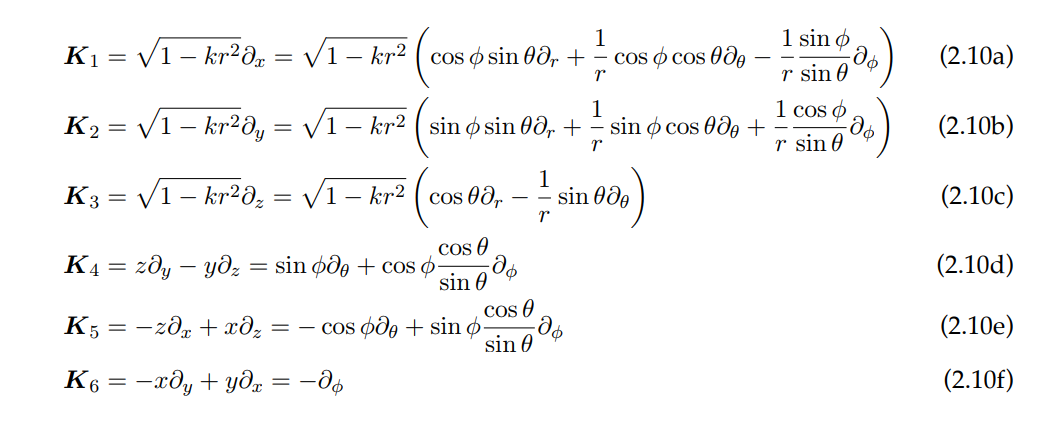
\includegraphics[width=0.7\linewidth]{gfx/CosmologyKillingVectorFields}
	\caption{}
	\label{fig:cosmologykillingvectorfields}
\end{figure}

in Cartesian and polar coordinates, respectively. The Killing condition \ref{eq:Killingeq}, iterated over
these six vector fields, then constitutes a set of partial differential equations for the components of the spacetime geometry tensor field $G$ in a choice of coordinates. Its solution
is, by definition, a tensor field that fulfills cosmological symmetries.

\begin{statements}
	Tracing the cosmological Killing vector fields foliates spacetime.
\end{statements}
We note here that the cosmological Killing vector fields give rise to a foliation of
our spacetime manifold in spatial hypersurfaces $Σ_t$ with a time parameter $t$ already. This
becomes apparent when we choose any point on the manifold and follow the integral
curves traced by the Killing vector fields that pierce through this point. Any two points on
the manifold connected by this procedure lie on the same spatial hypersurface. These vector
fields allow for a choice of chart where following any of their integral curves never
changes the coordinate we denoted as $w$ above and that we may now refer to as cosmic
time $t$. They still allow for reparametrizations $t → t^\prime$ of this coordinate however, that we
can describe through a lapse function $N(t)=\frac{\md t^\prime}{\md t}$.\\
Now with a set of Killing vector fields at hand that represent the cosmological symmetries, constructing a symmetric geometry reduces to the exercise of solving the Killing
condition \ref{eq:Killingeq} for it.\\
\\
The standard cosmological FLRW metric arises as the solution of the Killing condition \ref{eq:Killingeq}
for a Lorentzian metric geometry $g$
\begin{equation}
	0=K^m_i  \partial_m g^{ab} - 2 g^{m (a} \partial_m K^{b)}_i,
\end{equation}
where the $\mathbf{K}_i$ denote the six cosmological Killing vector fields as found above. This is a set of ten
partial differential equations for each of the six Killing vector fields. It is the Lie derivative \ref{eq:Killingeq} for a symmetric tensor field $g^{ab}$ written in components.
\\
\\
We choose a time coordinate and spatial polar coordinates $(t, r, θ, ϕ)$ to first solve the set
of equations for the metric components $g^{ab}$ and their derivatives $∂_mg^{ab}$, where we treat the $g^{ab}$ and $∂_mg^{ab}$ as independent variables. Solving the set of equations
then leaves only two metric components and both their derivatives by the time coordinate
undetermined. With these components chosen as $g_{tt}$ and $g_{rr}$, the remaining variables
solve to
\begin{figure}[h!]
	\centering
	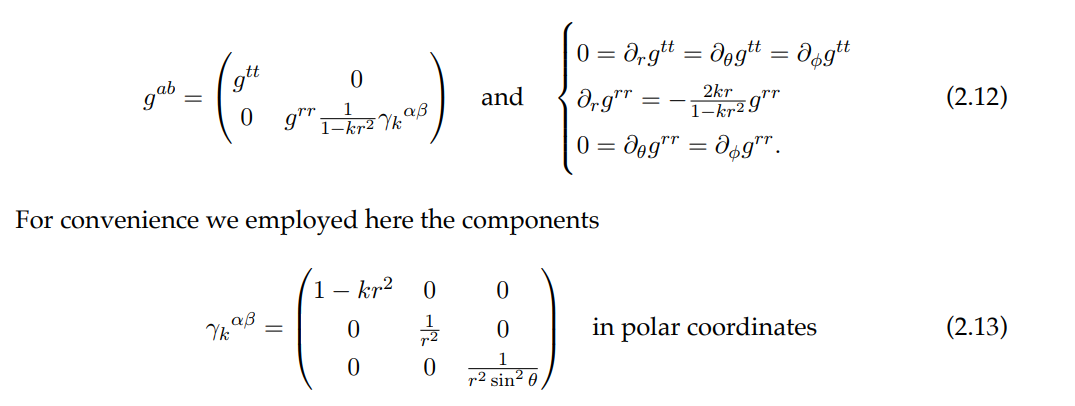
\includegraphics[width=0.7\linewidth]{gfx/FLRWmetricviaKilling}
	\caption{}
	\label{fig:flrwmetricviakilling}
\end{figure}
of a three dimensional Riemannian metric of constant curvature to abbreviate the notation. Note that we will also make use of its inverse $γ_{kαµ}γ^{k
µβ} = δ^\beta_α$
and its determinant $γ_k ≡ \det (
γ{kαβ})$.\\
\\
Now we are only left with solving the partial differential equations, in the figure the upper equations. They have
the solution
\begin{equation}
	g_{tt}=C_1(t) \qquad g_{rr} = -C_2(t) (1-kr^2)
\end{equation}
where two free functions $C_1(t)$ and $C_2(t)$ arise from the integration. Only the condition that the metric be Lorentzian constrains these functions, requiring that both be non-negative. To obtain a unique parametrization we therefore impose two conditions that
each define a metric degree of freedom:
\begin{enumerate}
	\item In a foliation of the spacetime manifold in spatial hypersurfaces we identify the
	lapse function
	\begin{equation}
		g^{tt} \stackrel{!}{=} \frac{1}{N^2(t)}.
	\end{equation}
	\item We compute the metric volume element
	\begin{equation}
\sqrt{-g} = N(t)C_2(t)^{-\frac{3}{2}}\sqrt{\gamma_k}
	\end{equation}
	and define a \emph{volume scale factor} $a(t)$ through the condition
	\begin{equation}
		\sqrt{-g}\stackrel{!}{=} N(t) a^3(t) \sqrt{\gamma_k}.
	\end{equation}
\end{enumerate}
Both conditions only serve to connect the arbitrary parametrization by $C_1(t)$ and $C_2(t)$ to
the conventional metric degrees of freedom $N(t)$ and $a(t)$ as
\begin{equation}
	C_1(t) = \frac{1}{N(t)} \quad and \quad C_2(t)=\frac{1}{a^2(t)}.
\end{equation}
With this choice of parameters we arrive precisely at the canonical FLRW metric
\begin{equation}
g^{ab} =
\begin{pmatrix}
\frac{1}{N^2(t)}&0\\
0& - \frac{1}{a^2(t)} \gamma^{\,\, \mu \nu}_k
\end{pmatrix}
\end{equation}
where indeed the scale factor $a(t)$ scales a three dimensional Riemannian metric of constant curvature $γ_k$. Note that in the literature the lapse function is usually chosen as $N(t) = 1$
in a particular choice of cosmic time.

\subsection{Conservation laws from Killing vector fields - More in depth}
Freely-falling particles and light rays both follow geodesics. For $\gamma$ a geodesic, then the projection of a Killing vector K on the tangent to the geodesic $\dot{\gamma}$ is constant along the geodesic,
\begin{equation}
\nabla_{\dot{\gamma}} \langle \dot{\gamma},K\rangle = 0.
\end{equation}
The constancy of $\langle \dot{\gamma},K\rangle$ along the geodesics means that each Killing vector field gives rise to a conserved quantity for freely-falling particles and light rays. Since a Killing vector field generates an isometry, this shows that 
\begin{statements}
	Symmetry transformations of the metric give rise to conservation laws.
\end{statements}

Killing fields are the infinitesimal generators of isometries; that is, flows generated by Killing fields are continuous isometries of the manifold  $\Leftrightarrow$ The flow generates a symmetry, in the sense that moving each point on an object the same distance in the direction of the Killing vector will not distort distances on the object.\\
E.g., in a \emph{static configuration}, in which nothing changes with time, the time vector will be a Killing vector, and thus the Killing field will point in the direction of forward motion in time.\\
\\
\\
A \emph{maximally symmetric space} is one
which possesses the largest possible number of Killing vectors, which on an $n$-dimensional
manifold is $n(n + 1)/2$. We will not prove this statement, but it is easy to understand at an
informal level. Consider the Euclidean space $\mR^n$ , where the isometries are well known to us:
translations and rotations. In general there will be $n$ translations, one for each direction we
can move. There will also be $n(n − 1)/2$ rotations; for each of $n$ dimensions there are $n − 1$
directions in which we can rotate it, but we must divide by two to prevent overcounting
(rotating $x$ into $y$ and rotating $y$ into $x$ are two versions of the same thing).
We therefore have
\begin{equation}
	n + \frac{n(n-1)}{2} = \frac{n(n+1)}{2}
\end{equation}
independent Killing vectors.
\subsection{Explicit Killing vectors}
For example in $\mR^2$ with metric $ds^2 = dx^2 +dy^2$ ,
independence of the metric components with respect to $x$ and $y$ immediately yields two
Killing vectors:
\begin{align}
	X^\mu &= (1,0) \nonumber \\
	Y^\mu &= (0,1) .
\end{align}
These clearly represent the two translations. The one rotation would correspond to the
vector $R = ∂/∂θ$ if we were in polar coordinates; in Cartesian coordinates this becomes
\begin{equation}
	R^{\mu} =(-y,x).
\end{equation}
These solve Killing's equation.\\
\\
Note that in $n ≥ 2$ dimensions, there can be more Killing vectors than dimensions. This
is because a set of Killing vector fields can be linearly independent, even though at any one
point on the manifold the vectors at that point are linearly dependent. It is trivial to show
(so you should do it yourself) that a linear combination of Killing vectors with constant
coefficients is still a Killing vector (in which case the linear combination does not count as
an independent Killing vector), but this is not necessarily true with coefficients which vary
over the manifold. You will also show that the commutator of two Killing vector fields is a
Killing vector field; this is very useful to know, but it may be the case that the commutator
gives you a vector field which is not linearly independent (or it may simply vanish).


















\section{Differential forms}
Differential $p$-forms are totally antisymmetric tensors of rank $(0,p)$.\\
The \emph{exterior product} $\wedge$ is defined by 
\begin{equation}
\wedge:\bigwedge^p \times \bigwedge^q \rightarrow \bigwedge^{p+q}, (\omega, \eta) \mapsto \omega \wedge \eta = \frac{(p+q)!}{p!q!} \mathcal{A}(\omega\otimes \eta),
\end{equation}
where $\mathcal{A}$ is the alternation operator
\begin{equation}
	(\mathcal{A}t)(v_1,\dots,v_p) = \frac{1}{p!} \sum_{\pi} \mathrm{sgn}(\pi) t(v_{\pi(1)}, \dots, v_{\pi(p)}).
\end{equation}
This operator we use to symmetrize or antisymmetrize tensors. To \emph{symmetrize}, we take the sum of all permutations of the relevant indices
and divide by the number of terms:
\begin{equation}
	T^{\sigma}_{(\mu_1 \dots \mu_n)\rho} = \frac{1}{n!} \left(T^{\sigma}_{\mu_1 \dots \mu_n \rho} + \mathrm{sum\,over\,permutations\,of\,indices\,} \mu_1 \dots \mu_n\right),
\end{equation}
while \emph{antisymmetrization} comes from the alternating sum:
\begin{equation}
T^{\sigma}_{[\mu_1 \dots \mu_n]\rho} = \frac{1}{n!} \left(T^{\sigma}_{\mu_1 \dots \mu_n \rho} + \mathrm{alternating\,sum\,over\,permutations\,of\,indices\,} \mu_1 \dots \mu_n\right).
\end{equation}
By “alternating sum” we mean that permutations which are the result of an odd number of
exchanges are given a minus sign, thus
\begin{equation}
	T_{[\mu \nu \rho] \sigma} = \frac{1}{6} \left[T_{\mu \nu \rho \sigma } - T_{\mu \rho \nu \sigma}  +T_{\rho \mu \nu  \sigma} -T_{\nu \mu \rho  \sigma} +T_{\nu \rho \mu \sigma}-T_{\rho \nu \mu \sigma} \right].
\end{equation}

On the vector space $\bigwedge$ of differential forms, the wedge product defines an \emph{associative, skew-commutative Grassman algebra},
\begin{equation}
	\omega \wedge \eta = (-1)^{pq} \eta \wedge \omega, \quad \omega \in \bigwedge^p, \eta \in \bigwedge^q.
\end{equation}
Given a $p$-form $A$ and a $q$-form $B$, we can form a $(p + q)$-form known as the wedge
product $A \wedge B$ by taking the antisymmetrized tensor product:
\begin{equation}
	(A\wedge B)_{\mu_1 \dots \mu_{p+q}} = \frac{(p+q)!}{p! q!} A_{[\mu_1 \dots \mu_p} B_{\mu_{p+1} \dots \mu_{p+1}]}.
\end{equation}
Thus, for example, the wedge product of two 1-forms is
\begin{equation}
	(A \wedge B)_{\mu \nu} = 2 A_{[\mu} B_{\nu]} = A_{\mu} B_{\nu} - A_{\nu} B_{\mu}.
\end{equation}



A basis for the $p$-forms is $\md x^{i_1} \wedge \dots \wedge \md x^{i_p}$, which shows that
\begin{equation}
	\dim{\bigwedge^p} = 
	\begin{pmatrix}
	n\\
	p
	\end{pmatrix}\qquad 
i \leq i_1 < \dots < i_p \leq n,
\end{equation}
where $\{\md x^i\}$ has $i\in \{1,\dots,n\}$ basis of $V^*$. So at a point on a 4-dimensional spacetime there is one linearly independent 0-form, four
1-forms, six 2-forms, four 3-forms, and one 4-form. There are no p-forms for p > n, since all
of the components will automatically be zero by antisymmetry.\\
\\
The \emph{interior product} $i_v$ is defined by 
\begin{equation}
	i:TM\times \bigwedge^p \rightarrow \bigwedge^{p-1}, (v,w) \mapsto i_v(w) =w(v,\dots) \Leftrightarrow (i_v w)_{i_2 \dots i_p} = v^j w_{j i_2 \dots i_p}.
\end{equation}
The \emph{exterior derivative} turns $p$-forms $w$ into $(p+1)$-forms $\md w$,
\begin{equation}
	\md : \bigwedge^p \rightarrow \bigwedge^{p+1}, \quad \omega \mapsto \md \omega = (p+1) \mathcal{A}(\nabla \omega).
\end{equation}
Thus, it also turns a $p$ tensor into a $(p+1)$ tensor, being unaffected of the curvature of our space. As it also formulated for the covariant derivative of tensors under the connection section, one can see this property by simply noting that the partial derivatives used to define the exterior derivative can be replaced with covariant derivatives, because the contribution of the affine connection coefficients that appear in the covariant derivatives vanish upon antisymmetrization.\\
Due to the symmetry of the Levi-Civita connection, the components of the exterior derivative are given by partial derivatives,
\begin{equation}
	(\md \omega)_{i_1,\dots,i_{p+1}} = (p+1) \partial_{[i_1} \omega_{i_2 \dots i_{p+1}]}.
\end{equation}
Equivalently with a use of basis,
\begin{align}
	\omega &= \omega_{i_1 \dots i_p} \md x^{i_1} \wedge \dots \wedge \md x^{i_p}, \\
	\md \omega &= \md \omega_{i_1 \dots i_p} \wedge \md x^{i_1} \wedge \dots \wedge \md x^{i_p},
\end{align}
where the differentials are wedged from the left. The simplest example is the gradient, which is the exterior derivative of a 1-form $(\md \phi)_{\mu} = \partial_{\mu}\phi$. The reason why the exterior derivative deserves special attention is that it is a tensor, even in
curved spacetimes, unlike its cousin the partial derivative.\\
Note that in general an exact $p$-form $t$ is not unique, given one such $t$, the most general $p$-form satisfying the exactness equation is of the form
\begin{equation}
	t^\prime = t + \md u \qquad u\in\bigwedge^{\quad \quad \quad (p-1)}.
\end{equation}
For instance, if the vector potential of the field strength tensor $F\munu$, hence $A_\alpha$, is one vector potential whose curl is $F_{\alpha \beta}$, then the most general such vector potential is given by the "gauge transformation":
\begin{equation}
	A^\prime_\alpha = A_\alpha + \partial_\alpha \Phi, \qquad \Phi \in \bigwedge^{\;\;0}.
\end{equation}





\subsection{Detour- de Rham Cohomology -- TO EXPAND}
We define a $p$-form $A$ to be \emph{closed} if $\md A = 0$,
and \emph{exact} if $A = \md B$ for some $(p − 1)$-form $B$. Obviously, all exact forms are closed, but the
converse is not necessarily true. On a manifold $M$, closed $p$-forms comprise a vector space
$Z^p (M)$, and exact forms comprise a vector space $B^p (M)$. Define a new vector space as the
closed forms modulo the exact forms:
\begin{equation}
	H^p(M) = \frac{Z^p(M)}{B^p(M)}.
\end{equation}
This is known as the \emph{$p$th de Rham cohomology vector space}, and depends only on the
topology of the manifold $M$. (Minkowski space is topologically equivalent to $\mR^4$ , which is
uninteresting, so that all of the $H^p (M)$ vanish for $p > 0$; for $p = 0$ we have $H^0 (M) = \mR$.
Therefore in Minkowski space all closed forms are exact except for zero-forms; zero-forms
can’t be exact since there are no $n$−1-forms for them to be the exterior derivative of.) It is
striking that information about the topology can be extracted in this way, which essentially
involves the solutions to differential equations. The dimension $b_p$ of the space $H^p (M)$ is
called the $p$th \emph{Betti number} of $M$, and the \emph{Euler characteristic} is given by the alternating
sum
\begin{equation}
	\chi(M) = \sum_{p=0}^{n} (-1)^p b_p.
\end{equation}
Cohomology theory is the basis for much of modern differential topology.



\subsection{Hodge star operator}
The  \emph{Hodge star operator} turns a $p$-form into an $(n-p)$- form,
\begin{equation}
	*:\bigwedge^p \rightarrow \bigwedge^{n-p}, \omega \mapsto * \omega,
\end{equation}
i.e. mapping $\omega$ to “$\omega$ dual”. Unlike our other operations on forms, the Hodge dual does depend
on the metric of the manifold (which should be obvious, since we had to raise some indices
on the Levi-Civita tensor in order to define it). Two facts on the Hodge dual: First, “duality” in the sense of Hodge is different than the
relationship between vectors and dual vectors, although both can be thought of as the space
of linear maps from the original space to $\mR$. Notice that the dimensionality of the space of
$(n − p)$-forms is equal to that of the space of $p$-forms, so this has at least a chance of being
true. In the case of forms, the linear map defined by an $(n − p)$-form acting on a p-form is
given by the dual of the wedge product of the two forms. Thus, if $A^{(n−p)}$ is an $(n − p)$-form
and $B^{(p)}$ is a $p$-form at some point in spacetime, we have
\begin{equation}
	*(A^{(n-p)}  \wedge B^{(p)}) \in \mR.
\end{equation}
The second fact concerns differential forms in 3-dimensional Euclidean space. The Hodge
dual of the wedge product of two 1-forms gives another 1-form:
\begin{equation}
	*(U\wedge V)_i = \epsilon^{\; jk}_i U_j V_k.
\end{equation}
(All of the prefactors cancel.) Since 1-forms in Euclidean space are just like vectors, we have
a map from two vectors to a single vector. You should convince yourself that this is just the
conventional cross product, and that the appearance of the Levi-Civita tensor explains why
the cross product changes sign under parity (interchange of two coordinates, or equivalently
basis vectors). This is why the cross product only exists in three dimensions — because only
in three dimensions do we have an interesting map from two dual vectors to a third dual
vector.
\\
\\
If $\{\md x^i\}$ is the basis of the dual space $T^*_p M$, then
\begin{equation}
	*(\md x^{i_1} \wedge \dots \wedge \md x^{i_p}) = \frac{\sqrt{|g|}}{(n-p)!} \epsilon^{i_1 \dots i_p}_{\quad \quad \quad i_{p+1} \dots i_n} \md x^{i_{p+1}} \wedge \dots \wedge \md x^{i_n},
\end{equation}
where the Levi-Civita tensor is only covariantly defined, i.e. $\epsilon_{i_1 \dots i_p} = \pm 1$ and indices have to be pushed up by $g^{\mu \nu} = (g_{\mu \nu})^{-1}$.
Here you symmetrize if the components are not in perfect order, i.e. for $\{x^0=c t ,r,\vartheta, \varphi\}$ one has
\begin{equation}
	*(\md \vartheta \wedge \varphi) = \frac{\sqrt{\abs{g}}}{(4-2)!} \left[\epsilon^{\vartheta \varphi}_{ct,r} c \md t\wedge \md r + \epsilon^{\vartheta \varphi}_{r,ct} \md r\wedge c\md t\right]=\frac{c \md t \wedge \md r}{r^2 \sin\vartheta}.
\end{equation}\\
For the orthonormal basis $\{e^i\}$ of $TM$,
\begin{equation}
	*(e^{i_1} \wedge\dots \wedge e^{i_p}) = e^{i_{p+1}} \wedge \dots \wedge e^{i_n}.
\end{equation}
As an intriguing aside, Hodge duality is the basis for one of the hottest topics in theoretical
physics today. It’s hard not to notice that the equations 
\begin{equation}
\md F = 0
\end{equation}
and 
\begin{equation}
\md (*F) = 4 \pi (* J)
\end{equation} look very similar.
Indeed, if we set $J_μ = 0$, the equations are invariant under the “duality transformations”
\begin{align*}
	F &\rightarrow *F\\
	*F & \rightarrow -F.
\end{align*}
We therefore say that the vacuum Maxwell’s equations are duality invariant, while the invariance is spoiled in the presence of charges. We might imagine that magnetic as well as electric monopoles existed in nature; then we could add a magnetic current term $4π(∗J_M )$ to the
right hand side of $\md F=0$, and the equations would be invariant under duality transformations
plus the additional replacement $J ↔ J_M$ . Long
ago Dirac considered the idea of magnetic monopoles and showed that a necessary condition
for their existence is that the fundamental monopole charge be inversely proportional to the fundamental electric charge. Now, the fundamental electric charge is a small number;
electrodynamics is “weakly coupled”, which is why perturbation theory is so remarkably
successful in quantum electrodynamics (QED). But Dirac’s condition on magnetic charges
implies that a duality transformation takes a theory of weakly coupled electric charges to a
theory of strongly coupled magnetic monopoles (and vice-versa). Unfortunately monopoles
don’t exist (as far as we know), so these ideas aren’t directly applicable to electromagnetism;
but there are some theories (such as supersymmetric non-abelian gauge theories) for which
it has been long conjectured that some sort of duality symmetry may exist. If it did, we
would have the opportunity to analyze a theory which looked strongly coupled (and therefore
hard to solve) by looking at the weakly coupled dual version. Recently work by Seiberg and
Witten and others has provided very strong evidence that this is exactly what happens in
certain theories. The hope is that these techniques will allow us to explore various phenom-
ena which we know exist in strongly coupled quantum field theories, such as confinement of
quarks in hadrons.


\subsection{Codifferential}
The \emph{codifferential} is a differentiation lowering the order of a $p$-form by one,
\begin{equation}
	\delta:\bigwedge^p \rightarrow \bigwedge^{p-1},\; \omega \mapsto \delta \omega = \mathrm{sgn}(g)\; (-1)^{n(p+1)} (*\md *)(\omega).
\end{equation}
It generalises the divergence:
\begin{equation}
	(\delta \omega)^{i_1 \dots i_{p-1}} = \frac{1}{\sqrt{|g|}} \partial_k \left(\sqrt{|g|} \omega_{k i_1 \dots i_{p-1}}\right).
\end{equation}


\subsection{Conventional differential operators via forms}
How can the exterior derivative and the co-differential be used to express the conventional
differential operators on vector fields, i.e. the curl, the divergence, and the Laplacian?\\
If $ω$ is the 1-form that belongs to the vector field $v$, i.e. $ω = v^{\flat} ∈ \bigwedge^{\;\;1}$ , its curl is given by $∗\md ω$,
i.e. the Hodge dual of the external derivative
\begin{equation}
	\mathrm{curl}\omega=*\md\omega, \quad \mathrm{curl} v=\left(*\md v^\flat\right)^\sharp.
\end{equation}
 The divergence of $ω$ is given by $δω$, i.e. the
co-differential:
\begin{equation}
	\mathrm{div}\omega=\nabla^\mu \omega_\mu = \delta \omega \quad \nabla_a\omega_b=\abs{g}^{-\half} \partial_a\left(\sqrt{\abs{g}} \omega_b\right),
\end{equation} 
or 
\begin{equation}
	\mathrm{div} v= \left(\delta v^\flat\right)^\sharp.
\end{equation}
The Laplacian of $ω$ is given by the Laplace-de Rham operator 
\begin{equation}
	\Delta \omega = (\md \circ \delta + \delta \circ \md) \omega,
\end{equation}
or
\begin{equation}
	\Delta v=\left[(\md \circ \delta + \delta \circ \md ) v^\flat\right]^\sharp.
\end{equation}
Then, for a function like the pressure $p$, one has
\begin{equation}
	g^{μα} ∇_α p = g^{μα} ∂_α p = g^{μα} (\md p)_α = (dp^\sharp)_μ = (\grad p)_μ .
\end{equation}








\section{Integrals}
The \emph{canonical volume form} on a pseudo-Riemannian manifold $(M,g)$ is defined by
\begin{equation}
	\eta = \sqrt{|g|} \md x^1 \wedge \dots \wedge \md x^n \quad \in \bigwedge^n.
\end{equation}
The integration of $n$-forms $\omega=f(x_1,\dots,x_n) \md x^1 \wedge \dots \wedge \md x^n$ over domains $D\subset M$ is coordinate independent and defined by
\begin{equation}
	\int_D \omega = \int_D f(x_1, \dots, x_n) \md x^1 \wedge \dots \wedge \md x^n.
\end{equation}
$\Rightarrow$ Functions $f$ are integrated by means of the canonical volume form,
\begin{equation}
	\int_D f \eta =\int_D f \sqrt{|g|} \md x^1 \wedge \dots \wedge \md x^n.
\end{equation}
\begin{mybox}{Stokes' theorem}
	Let $M$ be an $n$-dimensional manifold and the region $D\subset M$ have a smooth boundary $\partial D$ such that $\bar{D} = D \cup \partial D$ is compact. Then, for every $(n-1)$-form $\omega$, we have 
	\begin{equation}
		\int_D \md \omega = \int_{\partial D} \omega.
	\end{equation}

\end{mybox}

\begin{mybox}{Gauss' theorem}
	Likewise, for a vector field $X\in TM$ on $M$ and $x^{\flat}$ the 1-form belonging to this vector field:
	\begin{equation}
	\int_D \delta x^{\flat} \eta = \int_{\partial D} *x^{\flat}.
	\end{equation}
\end{mybox}

The musical operators used here are isomorphisms between the tangent spaces of a manifold and their dual spaces given by the metric
\begin{equation}
	\flat : TM \rightarrow T^*M, v \mapsto v^{\flat}, v^{\flat}_i =g_{ij} v^j,
\end{equation}
and similarly by the inverse of the metric,
\begin{equation}
	\#:T^*M \rightarrow TM, \omega \mapsto \omega^{\#}, \; (\omega^{\#})^i = g^{ij} \omega_j.
\end{equation}
Like $\flat$ lowers a note by a semitone in music, the $\flat$ operator lowers the index of vector components and thus turns then into dual vector components.. Analogously, $\#$ raises notes by semitones in music, and indices of dual-vector components.




\section{Frame fields in GR and the Tetrad formalism, "tetrad"="vierbein"="frame field"}
The tetrad formalism is an approach to general relativity that generalizes the choice of basis for the tangent bundle from a coordinate basis to the less restrictive choice of a local basis, i.e. a locally defined set of four linearly independent vector fields called a \emph{tetrad}.\\
The tetrad basis is chosen: a set of four independent vector fields
\begin{equation}
	e_a = e^{\mu}_a \partial_{\mu}, \quad \mathrm{for} \quad a=0,1,2,3,
\end{equation}
hat together span the 4D vector tangent space at each point in spacetime. Note that $e_0$ is a timelike vector field and $e_i$ is a spacelike vector field. Dually, a tetrad determines (and is determined by) a dual co-tetrad—a set of four independent covectors (1-forms)
\begin{equation}
	\theta^a = \theta^a_{\mu} \md x^{\mu}, \quad \theta^a \equiv e^a,
\end{equation}
such that $\theta^a(e_b) = \theta^a_{\mu} \theta^{\mu}_b=e^a_{\mu} e^{\mu}_b = \delta^a_b$.
A tetrad is specified by its coefficients $e^{\mu}_a$ w.r.t. a coordinate basis, despite the fact that the choice of a tetrad does not actually require the additional choice of a set of (local) coordinates $x^{\mu}$.\\
\\
In the tetrad formalism, all tensors are represented i.t.o. a chosen basis, vector or covector basis, by expressing them as linear combinations of numbers of the (co)tetrad. Popular tetrad bases include orthonormal tetrads and null tetrads, where the latter are composed of four null vectors (used in radiation problems).
\\
\\
Physical interpretation:\\
\textbf{Frame fields always correspond to a family of ideal observers immersed in the given spacetime; the integral curves of the timelike unit vector field are the worldlines of these observers, and at each event along a given worldline, the three spacelike unit vector fields specify the spatial triad carried by the observer. The triad may be thought of as defining the spatial coordinate axes of a local laboratory frame, which is valid very near the observer's worldline.}\\

In general, the worldlines of these observers need not be timelike geodesics. If any of the worldlines bends away from a geodesic path in some region, we can think of the observers as test particles that accelerate by using ideal rocket engines with a thrust equal to the magnitude of their acceleration vector. Alternatively, if our observer is attached to a bit of matter in a ball of fluid in hydrostatic equilibrium, this bit of matter will in general be accelerated outward by the net effect of pressure holding up the fluid ball against the attraction of its own gravity. Other possibilities include an observer attached to a free charged test particle in an electrovacuum solution, which will of course be accelerated by the Lorentz force, or an observer attached to a spinning test particle, which may be accelerated by a spin–spin force.\\

It is important to recognize that frames are geometric objects. That is, vector fields make sense (in a smooth manifold) independently of choice of a coordinate chart, and (in a Lorentzian manifold), so do the notions of orthogonality and length. Thus, just like vector fields and other geometric quantities, frame fields can be represented in various coordinate charts. Computations of the components of tensorial quantities, with respect to a given frame, will always yield the same result, whichever coordinate chart is used to represent the frame.\\
\\ 
The standard formalism of GR consists simply of using the coordinate tetrad in the tetrad formalism. The coordinate tetrad is the canonical set of vectors associated with the coordinate chart and is commonly denoted $\{\partial_{\mu}\}$, whereas the dual cotetrad is denoted $\{\md x^{\mu} \}$.\\
In the tetrad formalism, instead of writing tensor equations out fully (including $e_a,\theta^a$ and $\otimes$) only components of the tensors are mentioned, e.g. the metric is written as "$g_{ab}$".\\
\\
Changing tetrads is a routine operation in the standard formalism, as it is involved in every coordinate transformation (i.e., changing from one coordinate tetrad basis to another). Switching between multiple coordinate charts is necessary because, except in trivial cases, it is not possible for a single coordinate chart to cover the entire manifold. Changing to and between general tetrads is much similar and equally necessary (except for parallelizable manifolds). Any tensor can locally be written in terms of this coordinate tetrad or a general (co)tetrad. For example, the metric can be written as
\begin{equation}
	g=g_{\mu \nu} \md x^{\mu} \md x^{\nu}, \quad \mathrm{where} \quad g_{\mu \nu} = g(\partial_{\mu},\partial_{\nu}).
\end{equation}
For an arbitrary cotetrad (use $e^a \equiv \theta^a$ dual to $e_a$)
\begin{equation}
	g=g_{ab} e^a e^b, \qquad \mathrm{where} \quad g_{ab} = g(e_a,e_b).
\end{equation}
We can translate from a general co-tetrad to the coordinate co-tetrad by expanding the covector
\begin{align*}
	e^a &= e^a_{\mu} \md x^{\mu},\\
	\Rightarrow g=g_{ab}e^a e^b = g_{ab} e^a_{\mu} e^b_{\nu} \md x^{\mu} \md x^{\nu} &\stackrel{!}{=} g_{\mu \nu} \md x^{\mu} \md x^{\nu} \\
	\Leftrightarrow g_{\mu \nu} &= g_{ab} e^a_{\mu} e^b_{\nu}.
\end{align*}
Likewise expanding $\md x^{\mu}=e^{\mu}_a e^a$ w.r.t. the general tetrad, we get
\begin{align*}
	g&= g_{\mu \nu} \md x^{\mu} \md x^{\nu} = g_{\mu \nu} e^{\mu}_a e^a e^{\nu}_b e^b \\
	&=g_{ab} e^a e^b \\
	\Leftrightarrow g_{\mu \nu} e^{\mu}_a e^{\nu}_b &=g_{ab}.
\end{align*}
Be \emph{careful}:\\
The manipulation with tetrad coefficients shows that abstract index formulas can, in principle, be obtained from tensor formulas with respect to a coordinate tetrad by "replacing greek by latin indices". However care must be taken that a coordinate tetrad formula defines a genuine tensor when differentiation is involved. Since the coordinate vector fields have vanishing Lie bracket (i.e. commute: $ \partial_{\mu} \partial_{\nu} =\partial_{\nu} \partial_{\mu}$ ), naive substitutions of formulas that correctly compute tensor coefficients with respect to a coordinate tetrad may not correctly define a tensor with respect to a general tetrad because the Lie bracket is non-vanishing:$[e_a,e_b]\neq 0$.\\
E.g:
\begin{equation}
	\bar{R}(X,Y) =\left(\nabla_X \nabla_Y - \nabla_Y \nabla_Y - \nabla_{[X,Y]} \right),
\end{equation}
in a coordiante tetrad this gives the tensor coefficients
\begin{equation}
	\bar{R}^{\mu}_{\nu \sigma \tau} = \md x^{\mu} \left[\left(\nabla_{\sigma} \nabla_{\tau} - \nabla_{\tau} \nabla_{\sigma}\right) \partial_{\nu}\right].
\end{equation}
The naive and  "greek to latin" substitution of this is 
\begin{equation}
	\bar{R}^a_{bcd} = e^a\left[\left(\nabla_c \nabla_d - \nabla_d \nabla_c\right)e_b\right],\quad \mathrm{WRONG}
\end{equation}
is \emph{incorrect} because for fixed $c$ and $d$, $\left(\nabla_c \nabla_d - \nabla_d \nabla_c\right)$ is a first order differential operator rather than a zeroth order operator which defines a tensor coefficient. Substituting a general tetrad basis, we find the proper definition of $\bar{R}$ in abstract index notation:
\begin{equation}
	\bar{R}^a_{bcd} = e^a\left[\left(\nabla_c \nabla_d - \nabla_d \nabla_c - f^{\;\; e}_{cd} \nabla_e\right) e_b\right],
\end{equation}
where $\left[e_a,e_b\right]=f^{\; \; c}_{ab} e_c$.
\\
\\
Abstract index notation: $V$ a vector space, then for $(2,0)$-tensor $h \in V^* \otimes V^*$, or also
\begin{equation}
	\bar{R} = \bar{R}^{\; \; \; d}_{abc} \in \left(V^* \otimes V^* \otimes V^* \otimes V\right),
\end{equation}
therefore representing how covariant indices,i.e. $d$, represent the tensor swallowing one dual-vector (since $V$) and the contravariant indices, i.e. $a,b,c$, represent the tensor swallowing three vectors (since $V^* \otimes V^* \otimes V^*$).
\subsection{On the tetrad formalism - Weinberg}
The method employed by general covariance to port theories from SR to GR actually works only for objects that behave like tensors under Lorentz transformation, and not for the spinor fields. (Mathematically, this is because the tensor representation of the group GL(4) of general linear $4\times4$ matrices behave like tensors under the subgroup of Lorentz transformations, but there are no representations of GL(4), or even "representations up to a sign", which behave like spinors under the Lorentz subgroup.) How then can we incorporate spinors into GR?\\
The answer lies in a different approach to the problem of determining the effects of gravitation on physical systems.\\
To start, let us take advantage of the Principle of Equivalence, and at every point $X$ erect a set of coordinates $\xi^\alpha_X$ that are locally inertial at $X$. (Of course, it will not be possible to erect any \emph{single} coordinate system that is locally inertial everywhere, unless the space-time continuum is "flat".) The metric in any general noninertial coordinate system is then
\begin{equation}
g\munu (x)  = V^\alpha_\mu(x) V^\beta_\nu(x) \eta_{\alpha \beta}
\end{equation}
where 
\begin{equation}
	V^\alpha_\mu(X) \equiv \left(\frac{ \partial \xi^\alpha_X(x)}{\partial x^\mu}\right)_{x=X}.
\end{equation}
\marginpar{Note that in our formalism, this is equivalent to the expansions: $V^\mu= V^\mu_a \theta^a$ or $V_\mu = V^a_\mu e_a$.}
Note that we fix the locally inertial coordinates $\xi^\alpha_X$ once and for all at each physical point $X$, so when we change our general noninertial coordinates from $x^\mu$ to $x^{\prime \mu}$, the partial derivatives $V^\alpha_\mu$ change according to the role
\begin{equation}
	V^\alpha_\mu \rightarrow V^{\prime \alpha}_\mu = \frac{\partial x^\nu}{\partial x^{\prime \mu}} V^\alpha_\nu.
\end{equation}
Thus, we are to think of $V^\alpha_\mu$ as forming \emph{four} covariant vector fields, \emph{not} as a single tensor: This set of four vectors is known as a \emph{tetrad}, or \emph{vierbein}.
\begin{mybox}{Why are we changing to tetrad basis, my interpretation}
	Thus, The change to the tetrad basis is the change to a locally inertial system, i.e. to a freely falling system (RNC) where space appears to be flat. This basis generally depends on the coordinates from before, such that the basis changes from point to point on the manifold, thus this doesn't violate principle of equivalence as it is not one basis for all of the manifold but a smoothly changing basis, i.e. it is adapted to the manifold such that everything always looks flat/freely falling.
\end{mybox}
Now, given any contravariant vector field $A^\mu(x)$, we can use the tetrad to refer to its components at $x$ to the coordinate system $\xi^\alpha_X$ locally inertial at $x$:
\begin{equation}
	A^\alpha \equiv V^\alpha_\mu A^\mu.
\end{equation}
We are contracting a contravariant vector $A^\mu$ with four covariant vectors $V^\alpha_\mu$, so this has the effect of replacing the single four-vector $A^\mu$ with the four scalar $A^\alpha$. For general tensors:
\begin{equation}
	B^\alpha_\beta \equiv V^\alpha_\mu V^\nu_\beta B^\mu_\nu,
\end{equation}
here $V^\nu_\beta$ is just the tetrad, but with $\alpha$-index lowered with the Minkowski tensor and $\mu$-index raised with the metric tensor:
\begin{equation}
	V^\nu_\beta \equiv \eta_{\alpha \beta}g^{\mu \nu} V^\alpha_\mu.
\end{equation}
Note that the different bases are orthogonal
\begin{equation}
	\delta^\mu_\nu = V^\mu_\beta V^\beta_\nu, \qquad \delta^\alpha_\beta=V^\alpha_\mu V^\mu_\beta.
\end{equation}
The scalar components of the metric tensor are then simply:
\begin{equation}
	g_{\alpha \beta} \equiv V^\mu_\alpha V^\nu_\beta g\munu = \eta_{\alpha \beta}
\end{equation}
\subsubsection{Constructing an action - TO DO for QFT on curved spacetime }
How would we construct an action if we worked from the beginning with the scalars $V^\alpha,T_{\alpha\beta}$. There are now \emph{two} invariance principles which must be met in constructing a suitable matter action $S_M$:
\begin{enumerate}
	\item The action must be generally covariant, with all fields treated as scalars, except for the tetrad itself.
	\item The Principle of Equivalence requires that special relativity should apply in locally inertial frames, and in particular, that it should make no difference which locally inertial frame we choose at each point. Thus since our scalar field components $V^\alpha,T_{\alpha \beta}..$ are defined w.r.t. an arbitrarily chosen locally inertial coordinate system, the field equations and the action must be invariant w.r.t. a redefiniton of thee locally inertial coordinate systems at each point, or in other words, w.r.t. Lorentz transformations $\Gamma^\alpha_\beta(x)$ that can depend on position in space-time. The tetrad changes according to the same rules:
	\begin{equation}
		V^\alpha_\mu(x)\rightarrow\Gamma^\alpha_\beta(x) V^\beta_\mu(x).
	\end{equation}
	For an arbitrary field $\psi_n(x)$ given in tetrad formalism
	\begin{equation}
	\label{eq:Lorentzspinor}
		\psi_n(x) \rightarrow \sum_m [D(\Gamma(x))]_{nm} \psi_m(x)
	\end{equation}
	where $D(\Gamma)$ is a matrix representation of the Lorentz group (or at least of the infinitesimal Lorentz group).
\end{enumerate}
These two invariance principles lead to a dual classification of physical quantities. A \emph{coordinate scalar} or \emph{coordinate tensor} transforms as a scalar or tensor under changes in the coordinate system. A \emph{Lorentz scalar} or \emph{Lorentz tensor} or \emph{Lorentz spinor} transforms according to \ref{eq:Lorentzspinor}, with $D(\Lambda)$ the identity or a tensor representation or a spinor representation of the infinitesimal Lorentz group, under changes in the choice of the locally inertial coordinate frame. For instance, a field such as $A^\alpha = V^\alpha_\mu A^\mu$ is a coordinate scalar and a Lorentz vector, the Dirac field of the electron is a coordinate scalar and a Lorentz spinor, and the tetrad $V^\alpha_\mu$ is a coordinate vector and a Lorentz vector. To be physically acceptable, the matter action $S_M$ must be both a coordinate scalar and a Lorentz scalar.\\
\\
How is the gravitational field going to get into this sort of theory, when the coordinate-scalar components of the $g_{\alpha \beta}=\eta_{\alpha \beta}$ of the metric tensor are just the constants $\eta_{\alpha \beta}$?
\begin{mybox}{HOW GRAVITY APPEARS IN A THEORY - IMPORTANT}
	\emph{The answer is that gravitational tensor fields appear in the action because, and only because, of the necessity of introducing} \textbf{derivatives} \emph{into the theory.}
\end{mybox}
If it made sense to construct an action $S_M$ solely from fields, and not their derivatives, then it would only be necessary to choose some arbitrary Lorentz-invariant function $\mL(\psi(x))$ of various fields $\psi_n(x)$ (but not the tetrad), call them all coordinate scalars, and take the action as 
\begin{equation}
	S_M = \int \md^4 x \sqrt{g(x)} \mL(\psi(x)).
\end{equation}
This would then automatically be a coordinate scalar and a Lorentz scalar.
\begin{mybox}{Construction of a gravitational action}
	However, we saw in \ref{ch:GRtheory} that any physically sensible action must involve derivatives of physical quantities as well as the quantities themselves.
\end{mybox}
The tetrad field must enter into the action in such a way as to keep it a coordinate scalar and a Lorentz scalar despite the presence of derivatives.
\\
\\
\begin{mybox}{How to go over to QFT on curved background via tetrad formalism}
	Only summarizing here:\\
	The effects of gravitation on any physical system can be taken into account by writing down the matter action or the field equations that hold in special relativity, and then replacing all derivatives $\partial/\partial x^\alpha$ with the "covariant derivatives"
	\begin{equation}
	\mathcal{D}_\alpha \equiv V_\alpha^\mu \frac{\partial}{\partial x^\mu} + \half  \sigma^{\beta \gamma} V^\nu_\beta V^\mu_\alpha V_{\gamma \nu;\mu},
	\end{equation}
	where the $\sigma$ matrices are the ones appearing for infinitesimal Lorentz trafos 
\end{mybox}
\todo{Make a section on Lorentz group, trafos and infinitesimal Lorentz trafos as well as generators}
\todo{Make a section on QFT on curved background including the spin connection in modern fashion, via tetrad formalism}
This prescription yields a matter acction or fields equations that are invariant under general coordinate transformations, with $V^\mu_\alpha$ regarded as a four-vector and with all other fields regarded as scalar, and that aslo do not depend on how we choose locally inertial frames in defining the tetrad.\\
\\
How does one define the energy-momentum tensor in this formalism ?
The variation $\delta V^\mu_\alpha$ in the tetrad field will produce in the matter action a change:
\begin{equation}
	\delta I_M = \int \md^4 x \sqrt{g} U^\alpha_\mu \delta V^\mu_\alpha
\end{equation}
where $U^\alpha_\mu$ is a coordinate vector and a Lorentz vector.
\\
Define the energy-momentum tensor by
\begin{equation}
\label{eq:energymomentumTetradformalism}
T\munu \equiv V_{\alpha \mu} U^\alpha_\nu.
\end{equation}
As required, this is manifestly a coordinate tensor and a Lorentz scalar. To verify that \ref{eq:energymomentumTetradformalism} is a suitable energy-momentum tensor, we must also check that it is symmetric and that it is covariantly conserved. The symmetry property of the energy-momentum tensor is not at all obvious in the tetrad formalism, but must be derived from the invariance of the matter action under the infinitesimal Lorentz transformations (also under position dependent ones). To show that this energy-momentum tensor is conserved, one uses the invariance of the matter action under infinitesimal coordinate transformations. This definition therefore works.\\
Note however, that if the matter action were not invariant under position-dependent Lorentz transformations, then not only would $T\munu$ not be symmetric, but in consequence, it would also not be conserved. One again construct the total action for matter and gravitation 
\begin{equation}
	S=S_M+S_G
\end{equation}
and gets the field equations from them. These equations serve to determine only $g\munu$, leaving the tetrad determined only up to a Lorentz transformation. However, the invariance of the matter action under such position-dependent Lorentz transformations ensures that all tetrads associated with a given metric have the same physical effects.

\section{Cartan's structure equations}
Let $M$ be a differentiable manifold, $\{e_i\}$ an arbitrary basis for vector fields and $\{\theta^i\}$ an arbitrary basis for dual vector fields, or 1-forms, such that 
\begin{equation}
	\langle \theta^i,e_j\rangle = \delta^i_j.
\end{equation}
\begin{mybox}{Connection forms}
	In analogy to $\Gamma^i_{jk}$, we introduce the connection forms $\omega^j_i$ by
	\begin{equation}
		\nabla_v e_a = \omega^b_a(v) e_b.
	\end{equation}
	Since $\nabla_v e_i$ is a vector, $\omega^j_i(v) \in \mR$, and thus $\omega^j_i \in \bigwedge^1$ is a dual vector, or a one form.
\end{mybox}
\marginpar{The connection forms are sometimes referred to as spin connection, which comes from the fact that this can be used to take covari-
	ant derivatives of spinors, which is actually impossible using the conventional connection
	coefficients.}
\begin{align}
	\nabla_{\partial_k} \partial_j &=\Gamma^i_{kj} \partial_i = \omega^i_j(\partial_k)\partial_i \nonumber \\
	\Rightarrow \omega^i_{\;j} &= \Omega^i_{kj} \md x^k \quad \Leftrightarrow \quad \omega^i_{\;j} = \Gamma^i_{kj} \theta^k.
\end{align}
\marginpar{Where one uses in $\{e_i\}$, $\omega_{ij} \equiv g_{ik} \omega^k_{\;j}, \quad g_{ij} = g(e_i,e_j)$.}
They satisfy the antisymmetry relation, if and only if $\nabla g=0$ the connection is metric:
\begin{equation}
	\md g_{ij} = \omega_{ij} + \omega_{ji}.
\end{equation}
The covariant derivative of a dual basis vector is
\begin{align}
	\nabla_v \theta^i &= - \omega^i_{\;j} (v) \theta^i,\\
	\nabla \theta^i &= - \theta^j \otimes \omega^i_{\;j}.
\end{align}
Covariant derivatives of arbitrary vector $x=x^i e_i$ and dual vector $\alpha=\alpha_j \theta^j$ are then
\begin{equation}
	\nabla_v x = \langle \md x^i + x^j \omega^i_{\;j}, v\rangle e_i, \quad \nabla_v \alpha = \langle \md \alpha_i - \alpha_j \omega^j_{\; i},  v\rangle \theta^i,
\end{equation}
or
\begin{equation}
	\nabla x = e_i \otimes \langle \md x^i+x^j \omega^i_{\;j}\rangle, \quad \nabla \alpha = \theta^i \otimes (\md \alpha_i - \alpha_k \omega^k_{\;i}).
\end{equation}
\marginpar{In QFT, the connection forms are the field strengths $F_{\mu \nu} \Leftrightarrow$ curvature forms. All this translates to structure of gauge theories. See chapter 2.}

\begin{mybox}{Torsion and curvature form}
	The torsion $T(x,y)$ is a vector, which can be written in terms of the torsion forms $\Theta^i$ as 
	\begin{equation}
		T(x,y) = \Theta^i(x,y) e_i, \quad \Theta^i \in \bigwedge^2 \quad \Rightarrow \; \Theta^i(x,y) \in \mR.
	\end{equation}
	Similarly, express the curvature by the curvature forms $\Omega^i_{\; j} \in \bigwedge^2$,
	\begin{equation}
		\bar{R}(x,y)e_j = \Omega^i_{\;j}(x,y)e_i.
	\end{equation}
\end{mybox}

\begin{mybox}{Cartan's structure equations}
	In terms of the connection forms $\omega^i_{\; j}$. the torsion forms $\Theta^i$ and the curvature forms $\Omega^i_{\;j}$ are determined by Cartan's structure equations,
	\begin{align}
		\label{eq:cartanStructure}
		\Theta^i &= \md \theta^i + \omega^i_{\;j} \wedge \theta^j,\\
		\Omega^i_{\;j} &= \md \omega^i_{\;j} + \omega^i_{\;k} \wedge \omega^k_{\; j}.
	\end{align}
\end{mybox}
\begin{mybox}{Computing the curvature tensors}
	The Riemann tensor in components is then obtained via
	\begin{equation}
		\bar{R}^a_{bcd} = \Omega^a_b(e_c,e_d)
	\end{equation}
	such that the Ricci tensor is given by the contraction of the first and third component
	\begin{equation}
		R_{bc} = \Omega^a_b(e_a,e_c).
	\end{equation}
	The torsion tensor is given by
	\begin{equation}
		T^a_{bc} = \Theta^a (e_b,e_c).
	\end{equation}
\end{mybox}
In reading off the connection forms, always think of antisymmetrizing the form such that
\begin{equation} 
	\md g_{ab} =0 =\omega_{ab}+\omega_{ba} 
\end{equation}
holds. That is, use the antisymmmetrizer in reading the connection forms off:
\begin{equation}
	(\omega \wedge \eta)=\frac{(p+q)!}{p!q!} \mathcal{A}(\omega\otimes\eta)
\end{equation}
such that for example
\begin{equation}
	(\theta^i\wedge \theta^j)(e_a,e_b) =\left[\theta^i(e_a) \theta^j(e_b) - \theta^i(e_b) \theta^j(e_a)\right].
\end{equation}
The components of the torsion and curvature tensors are determined by 
\begin{align}
	\Theta^i &= \frac{1}{2} T^i_{jk} \theta^j \wedge \theta^k,\\
	\Omega^i_{\;j} &= \frac{1}{2}  \bar{R}^i_{jkl} \theta^k \wedge \theta^l.
\end{align}
Note that the connection forms obtained from Cartan's structure equations have to be antisymmetrized in $i,j$ to get the full connection form. ALWAYS CHECK. This antisymmetry comes about by the metric being Minkowskian. Constant form of the metric here implies that we always can raise and lower indices by simply introducing minus or plus signs where appropriate
\begin{equation*}
	A^i_{\;\;j} = \pm A^{\;\; j}_i.
\end{equation*}
\\
\bullet Normally we have connection forms without torsion, will require that it has to vanish.
$\stackrel{Cartan}{\Rightarrow} \md \theta^i = - \omega^i_{\;k} \wedge \theta^i \Rightarrow$ choose a dual basis $\theta^i$, take derivative and read off $\omega^i_k$.\\
Recipe:\\
Introduce basis such that $g_{ij}=\pm 1\Rightarrow \md g_{ij} = 0 = \omega_{ij}+\omega_{ij} \Rightarrow$ only $6 \omega_{ij}$ left $ \Rightarrow$ easy calculation vs $\Gamma^i_{jk}\Rightarrow$ Minkowskian calculation with 
\begin{equation}
	g = g_{\mu \nu} \md x^{\mu} \otimes \md x^{\nu} = \tilde{g}_{\mu \nu} \theta^{\mu} \otimes \theta^{\nu},
\end{equation}
choose $\theta^{\mu},\theta^{\nu}$ such that $\tilde{g}_{\mu \nu} = \pm 1$. With this choice, the metric has become Minkowskian.
\begin{mybox}{Geodesic equation in tetrad formalism}
	The geodesic equation in the tetrad formalism reads
	\begin{equation}
		0=\nabla_u u = u^a \omega^{\;\;b}_a (u) e_b + u(u^b) e_b.
	\end{equation}
	Now you can project vectors $\theta^c$ onto this equation to find the different components $c \in \{0,1,2,3\}$.
	\begin{equation}
		u(u^a) + u^b \omega^a_b (u)=0.
	\end{equation}
\end{mybox}
\begin{mybox}{How to change basis}
	Consider a vector being given in coordinate tetrad and wanting to find the corresponding vector in the corresponding general tetrad:
	\begin{equation}
		u=\tilde{u}^\mu \partial_\mu = u^a e_a.
	\end{equation}
	The components are then given by
	\begin{equation}
		u^0 = \theta^0(u) = \tilde{u}^0 \theta^0(\partial_0) + \tilde{u}^i \theta^0(\partial_i).
	\end{equation}
	The orthonormality of the two different tetrad basis $\partial_i$ and co-basis $\theta^a$ is not guaranteed. Therefore we make an ansatz to find the general basis which fits to this special general co-basis:
	\begin{equation}
		e_0 = A \partial_0, \; e_i = B \partial_i, \; \theta^0 = C\md x^0 ,\; \theta^j = D \md x^j.
	\end{equation}
	Now you use the orthonormality condition $\theta^a(e_b) = \delta^a_b$ and $\md x^\mu(\partial_\nu) = \delta^\mu_\nu$, which has to hold by definition, to determine the coefficients , by looking at 
	\begin{equation}
		1 \stackrel{!}{=} \theta^0(e_0) = AC \md x^0(\partial_0) = AC,
	\end{equation}
	and so forth. Usually, the coefficients $C,D$ are already known since you express the metric via the co-basis:
	\begin{equation}
		g=g\munu \md x^\mu \md x^\nu = g_{ab} \theta^a \theta^b \quad \Rightarrow \theta^0 = \dots \md x^0, \theta^i = \dots \md x^i,
	\end{equation}
	which simply then gives you the coefficients of the basis $e_a$ since you know the full basis $\partial_\mu$ and the full co-bases $\theta^b,\md x^\mu$.
\end{mybox}
\section{Comparison of gauge theories in particle physics with Riemannian geometry}
\label{subsec:GaugeTheoriesInterpretation}
We now have the means to compare the formalism of connections and curvature in Riemannian geometry to that of gauge theories in particle physics. In
both situations, the fields of interest live in vector spaces which are assigned to each point
in spacetime. In Riemannian geometry the vector spaces include the tangent space, the
cotangent space, and the higher tensor spaces constructed from these. In gauge theories,
on the other hand, we are concerned with “internal” vector spaces. The distinction is that
the tangent space and its relatives are intimately associated with the manifold itself, and
were naturally defined once the manifold was set up; an internal vector space can be of any
dimension we like, and has to be defined as an independent addition to the manifold. In
math lingo, the union of the base manifold with the internal vector spaces (defined at each
point) is a \emph{fiber bundle}, and each copy of the vector space is called the “fiber” (in perfect
accord with our definition of the tangent bundle).\\
Besides the base manifold (for us, spacetime) and the fibers, the other important ingredient in the definition of a fiber bundle is the “\emph{structure group},” a Lie group which acts
\marginpar{A more modern interpretation of the physical content of the original principle of general covariance is that the Lie group $GL(4,\mR)$ is a fundamental "external" symmetry of the world. Other symmetries, including "internal" symmetries based on compact groups, now play a major role in fundamental physical theories.}
on the fibers to describe how they are sewn together on overlapping coordinate patches.
Without going into details, the structure group for the tangent bundle in a four-dimensional
spacetime is generally $\mathrm{GL}(4, \mR)$, the group of real invertible 4 × 4 matrices; if we have a
Lorentzian metric, this may be reduced to the Lorentz group $SO(3, 1)$. Now imagine that
we introduce an internal three-dimensional vector space, and sew the fibers together with
ordinary rotations; the structure group of this new bundle is then $SO(3)$. A field that lives
in this bundle might be denoted $\phi^A (x^μ )$, where $A$ runs from one to three; it is a three-vector
(an \emph{internal one, unrelated to spacetime}) for each point on the manifold. We have freedom
to choose the basis in the fibers in any way we wish; this means that “physical quantities”
should be left invariant under local $SO(3)$ transformations such as
\begin{equation}
	\phi^A(x^{\mu}) \rightarrow \phi^{A^\prime} (x^\mu) = O^{A^\prime}_A(x^\mu) \phi^A(x^\mu),
\end{equation}
where $O^{A^\prime}_A (x^μ )$ is a matrix in $SO(3)$ which depends on spacetime. Such transformations
are known as \emph{gauge transformations}, and theories invariant under them are called “\emph{gauge
theories}”.\\
\\
For the most part it is not hard to arrange things such that physical quantities are
invariant under gauge transformations. The one difficulty arises when we consider partial
derivatives, $∂_μ \phi^A$ . Because the matrix $O^{A^\prime}_A (x^μ )$ depends on spacetime, it will contribute an
unwanted term to the transformation of the partial derivative. By now you should be able
to guess the solution: introduce a connection to correct for the inhomogeneous term in the
transformation law. We therefore define a connection on the fiber bundle to be an object
$A^{\;A}_{\mu\;\; B}$ , with two “group indices” and one spacetime index. Under GCT’s (We still have our usual
freedom to make changes in coordinates, which are called general coordinate transformations, or GCT’s.) it transforms as a
one-form, while under gauge transformations it transforms as
\begin{equation}
\label{eq:fibrebundleconnectiontrafo}
	A^{\;A^\prime}_{\mu \;\; B^\prime} =O^{A^\prime}_{\;A} O^{\;B}_{B^\prime}A^{\;A}_{\mu \;\;B}  -O^{\;\;C}_{B^\prime} \partial_{\mu} O^{A^\prime}_C.
\end{equation}
Beware: our conventions are so drastically different from those in the particle physics literature that I won’t even try to get them straight.) With this transformation law, the “\emph{gauge
covariant derivative}”
\begin{equation}
\label{eq:gaugecovderiv}
	D_\mu \phi^A = \partial_{\mu} \phi^A + A^{\;\,A}_{\mu \;\;B} \phi^B
\end{equation}
transforms “tensorially” under gauge transformations, as you are welcome to check. (In
ordinary electromagnetism the connection is just the conventional vector potential. No
indices are necessary, because the structure group $U(1)$ is one-dimensional.)
\\
It is clear that this notion of a connection on an internal fiber bundle is very closely
related to the connection on the tangent bundle, especially in the orthonormal-frame picture
we have been discussing. The transformation law \ref{eq:fibrebundleconnectiontrafo}, for example, is exactly the same
as the transformation law for the spin connection $\omega^a_b$. We can also define a curvature or
“field strength” tensor which is a two-form,
\begin{equation}
F^A_B = \md A^A_{\;B} + A^A_{\;C} \wedge A^C_{\;B}
\end{equation}
in exact correspondence with the second Cartan structure equation for the curvature form \ref{eq:cartanStructure}.\\
We can parallel transport things along paths, and
there is a construction analogous to the parallel propagator; the trace of the matrix obtained
by parallel transporting a vector around a closed curve is called a “\emph{Wilson loop}.”
We could go on in the development of the relationship between the tangent bundle and
internal vector bundles, but time is short and we have other fish to fry. Let us instead finish
by emphasizing the important \emph{difference} between the two constructions. The difference
stems from the fact that the tangent bundle is closely related to the base manifold, while
other fiber bundles are tacked on after the fact. It makes sense to say that a vector in the
tangent space at $p$ “points along a path” through $p$; but this makes no sense for an internal
vector bundle. There is therefore no analogue of the coordinate basis for an internal space —
partial derivatives along curves have nothing to do with internal vectors. It follows in turn
that there is nothing like the vielbeins, which relate orthonormal bases to coordinate bases.
The torsion tensor, in particular, is only defined for a connection on the tangent bundle, not
for any gauge theory connections; it can be thought of as the covariant exterior derivative
of the vielbein, and no such construction is available on an internal bundle. You should
appreciate the relationship between the different uses of the notion of a connection, without
getting carried away.










































\chapter{General Relativity - the Theory}

\label{ch:GRtheory}
\section{Introduction to General Relativity}
The experimentally well-established \emph{principle of equivalence}, stating the equivalence of inertial and gravitational mass, is the heuristic guiding principle of GR and has the following forms:
\begin{enumerate}
	\item The weaker and less precise statement is that the motion of a test body in a gravitational field is independent of its mass and composition.
	\item In a more precise form: In an arbitrary gravitational field no local non-gravitational experiment can distinguish a freely falling, non-rotating system from a uniformaly moving system in absence of the gravitational field $\rightarrow$ objects with different mass fall at the same speed under gravity.
\end{enumerate}

Where \emph{Freely falling frames of reference}:
It must be possible to introduce local, non-rotating, freely-falling frames of reference in which gravity is locally "transformed away".
The directions of motion of different freely-falling reference frames will generally not be parallel: E.g. Einstein elevators released at same height but different locations over Earth's surface.
\marginpar{A manifold with a metrix which is not positive definite is called pseudo-Riemannian, or Lorentzian if the metric has the signature of the Minkowski metric.}
\graffito{An outlook into the future of \texttt{classicthesis}.}
\subsection{Closer Look at the Equivalence Principle}
In other words:\\
The inertial mass clearly has a universal character, related to the resistance you feel when
you try to push on the object; it is the same constant no matter what kind of force is being
exerted 
\begin{equation}
\vec{f}=m_i \vec{a}.
\end{equation}
Gravitation on the other hand is
\begin{equation}
\vec{f}_G = -m_g \vec{\nabla} \Phi.
\end{equation}
On the face of it, $m_g$ has a very different character than $m_i$ ; it is a quantity specific to the
gravitational force. If you like, it is the “gravitational charge” of the body. Nevertheless,
Galileo long ago showed that the response of matter to gravitation was
universal — every object falls at the same rate in a gravitational field, independent of the
composition of the object.
\begin{mybox}{Weak Equivalence Principle}
In Newtonian mechanics this translates into the Weak Equivalence Principle (WEP), which is
simply
\begin{equation}
m_g = m_i
\end{equation}
for any object.
\end{mybox} 
An immediate consequence is that the behavior of freely-falling test particles
is universal, independent of their mass (or any other qualities they may have); in fact we have
\begin{equation}
\vec{a} =- \vec{\nabla} \Phi
\end{equation}
The WEP implies that there is no way to disentangle the effects of a gravitational field
from those of being in a uniformly accelerating frame, simply by observing the behavior of
freely-falling particles. This follows from the universality of gravitation; it would be possible
to distinguish between uniform acceleration and an electromagnetic field, by observing the
behavior of particles with different charges. But with gravity it is impossible, since the
“charge” is necessarily proportional to the (inertial) mass. To be careful, we should limit our claims about the impossibility of distinguishing gravity
from uniform acceleration by restricting our attention to “small enough regions of spacetime.”
The WEP can therefore be stated as “the laws of freely-falling particles are the same in a
gravitational field and a uniformly accelerated frame, in small enough regions of spacetime.”
In larger regions of spacetime there will be inhomogeneities in the gravitational field, which will lead to detectable tidal fields.
\\
\\
\begin{mybox}{Einstein Equivalence
	Principle, or EEP}
“In small enough regions of spacetime, the laws of physics reduce to
those of special relativity; it is impossible to detect the existence of a gravitational field."
\end{mybox}
\marginpar{Hence, $g\rightarrow\eta$ ?}
The EEP implies that gravity is inescapable — there is no such thing as a “gravitationally neutral
object” with respect to which we can measure the acceleration due to gravity. It follows
that “the acceleration due to gravity” is not something which can be reliably defined, and
therefore is of little use.
Instead, it makes more sense to \emph{define} “unaccelerated” as “freely falling,” and that is
what we shall do. This point of view is the origin of the idea that gravity is not a “force”
— a force is something which leads to acceleration, and our definition of zero acceleration is
“moving freely in the presence of whatever gravitational field happens to be around.”\\
The solution is to retain the notion of inertial frames, but to discard the hope that they
can be uniquely extended throughout space and time. Instead we can define \emph{locally inertial
	frames}, those which follow the motion of freely falling particles in small enough regions of
spacetime. This is the best we
can do, but it forces us to give up a good deal. For example, we can no longer speak with
confidence about the relative velocity of far away objects, since the inertial reference frames
appropriate to those objects are independent of those appropriate to us.
\subsection{Another look at the equivalence principle by Feynman}
\begin{statements} 
	The central idea of gravity, the most cogent fact about how it acts, is that weight and mass are exactly proportional, so that all objects accelerate under gravity at exactly the same rate, no matter what their constitution may be.
\end{statements}
The experiment of Eötvös showed how a centrifugal force added to a gravity force in such a way that the resultant was indistinguishable from a purely gravitational effect. The weightlessness in satellites is an example of a cancellation of gravitational forces by an acceleration. It is this possibility of cancellation which is the core of the principle of equivalence.\\
\\
In special relativity, extensive use is made of reference frames which are moving with a uniform velocity in a straight line. But, as soon as we allow the presence of gravitating masses anywhere in the universe, the concept of such truly unaccelerated motion becomes impossible, because there will be gravitational fields everywhere.\\
If we are performing experiments inside a box which is not in free fall, it will be possible to detect the presence of gravitation-like forces, by an experiment with masses coupled to springs for example. However, we cannot tell from inside the box whether we are accelerating relative to the nebulae, or whether the forces are due to masses in the neighbourhood:
\begin{mybox}{Equivalence principle, EP}
	It shall be impossible, by any experiment whatsoever performed inside such a box, to detect a difference between an acceleration relative to the nebulae and gravity. That is, an accelerating box in some gravitational field is indistinguishable from a stationary box in some different gravitational field.
\end{mybox}
\subsection{Consequences of principle of equivalence}
The principle of equivalence tells us that light falls in a gravitational field. If the box is accelerating, the light travels in a straight line in an unaccelerated system.\\
\\
The EP also tells us that clock rates are affected by gravity. Light which is emitted from the top of the accelerating box will look violet-shifted as we loom at it from the bottom. One way of describing this situation is to say that the time scale is faster at the top; time flows are diferent in different gravitational potentials, so that time flows are unequal in various parts of the world. How much is this time difference at various points in space ? To calculate it, we compare the time rates with an absolute time separation, defined i.t.o. the proper time $\md s$. Let us suppose that there are two events occuring at the top, which are reported to be a time $\md t$ apart; then
\begin{equation}
\phi = g h, \quad \md s = \md t(1 + \phi/c^2),
\end{equation}
in the limit of small velocities. The quantity $\phi$ is simply the potential difference between the location of the events, and the point of reference. A more careful computation gives us an expression good for all velocities 
\begin{equation}
\md s = \md t \sqrt{1+2 \phi/c^2}.
\end{equation}
\\
\\
\subsubsection{Equivalence Principle implies light deflection and gravitational redshift}
According to the equivalence principle, the downward gravitational acceleration felt in an
Einstein elevator cannot locally be distinguished from a constant upward acceleration of the
elevator with the same acceleration. Adopting the equivalence principle, one can thus assume
that the gravitational field is absent and that the elevator is constantly accelerated upward instead.
When the photon is received at the ceiling, the ceiling moves with a finite velocity compared to
the floor when the photon was emitted. The photon is thus Doppler shifted with respect to its
emission and is received with a longer wavelength.
\\
Note that Doppler shift in GR is defined by the change in frequency
\begin{equation}
\label{eq:dopplershiftgr}
\frac{\nu_s}{\nu_o} = \frac{g(k, u)|_s}{g(k, u)|_o},
\end{equation}
where $k$ is
the light’s four-wave vector, any distinction between Doppler shift and gravitational redshift has
no invariant meaning in general relativity.\\
Similarly, it can be concluded from the equivalence principle that light rays should be curved in
gravitational fields. Suppose that a horizontal light ray enters an Einstein elevator to the left and
leaves it at a later time to the right. As the light ray leaves the elevator, the elevator’s velocity
has increased so that in the rest frame of the elevator, it leaves at an angle downward from the
horizontal because of the aberration due to the finite speed of light.
\subsubsection{Equivalence Principle implies metric being a dynamical field}
The equivalence of inertial and gravitational mass led Einstein to the equivalence principle,
which says that it must be possible to introduce local, non-rotating, freely-falling frames of
reference in which gravity is locally “transformed away”. The directions of motion of different
freely-falling reference frames will generally not be parallel: Einstein elevators released at the
same height above the Earth’s surface but over different locations will fall towards the Earth’s
centre and thus approach each other. Replacing inertial frames by freely falling, non-rotating
frames of references leads to the idea that space-time is a four-dimensional manifold instead of
the “rigid”, four-dimensional Euclidean space.
In a freely-falling reference frame, special relativity must hold, implying that the Minkowskian
metric of special relativity must locally be valid. The same operation must be possible in all
freely-falling reference frames individually, but not globally. Thus, general relativity considers
the metric of the space-time manifold as a dynamical field.

\subsection{From Newton to Einstein}
 In
a significant change of perspective from regarding gravity as a force between point like
particles with mass, they instead follow straight lines through a curved geometry. Only
where these free-fall trajectories, or geodesics, cannot be sustained—for instance when the
surface of the Earth prevents us from falling through—do we experience a reaction. This
makes gravity locally indistinguishable from any inertial acceleration that we feel, for
instance, in an elevator accelerating upwards or in a car going around a corner. Closing
this reasoning, what induces the spacetime curvature in the theory of general relativity is
the matter and energy it carries. This makes even us slightly bend the spacetime around
us, so that objects and indeed also light are affected by our presence, and even more so
by more massive objects such as the planet Earth or the Sun.


\section{On our Path towards a curved Spacetime}
So far we have been talking strictly about physics, without jumping to the conclusion
that spacetime should be described as a curved manifold. It should be clear, however, why
such a conclusion is appropriate. The idea that the laws of special relativity should be
obeyed in sufficiently small regions of spacetime, and further that local inertial frames can
be established in such regions, corresponds to our ability to construct Riemann normal coordinates at any one point on a manifold — coordinates in which the metric takes its canonical
form and the Christoffel symbols vanish. The impossibility of comparing velocities (vectors)
at widely separated regions corresponds to the path-dependence of parallel transport on a
curved manifold. These considerations were enough to give Einstein the idea that gravity
was a manifestation of spacetime curvature.\\
\\
The principle of
equivalence tells us that the laws of physics, in small enough regions of spacetime, look like
those of special relativity. We interpret this in the language of manifolds as the statement
that these laws, when written in Riemannian normal coordinates $x^μ$ based at some point
$p$, are described by equations which take the same form as they would in flat space. The
simplest example is that of freely-falling (unaccelerated) particles. In flat space such particles
move in straight lines; in equations, this is expressed as the vanishing of the second derivative
of the parameterized path $x^μ (λ)$:
\begin{equation}
\frac{\md^2 x^\mu}{\md \lambda^2} = 0.
\end{equation}
According to the EEP, exactly this equation should hold in curved space, as long as the
coordinates $x^μ$ are RNC’s. What about some other coordinate system? As it stands, this is not an equation between tensors. However, there is a unique tensorial equation which
reduces to this when the Christoffel symbols vanish; it is the geodesic equation
\begin{equation}
\frac{\md^2 x^\mu}{\md \lambda^2} + \Gamma^\mu_{\rho \sigma} \frac{\md x^\rho}{\md \lambda} \frac{\md x^\sigma}{\md \lambda} = 0.
\end{equation}
In general relativity, therefore, free particles
move along geodesics; we have mentioned this before, but now you know why it is true.
\marginpar{General relativity keeps the light-cone structure of special relativity, even thought its rigidity is given up: the orientation of light cones can vary across space-time.}.

\section{Newtonian limit:}
We define the “\emph{Newtonian limit}” by
three requirements
\begin{enumerate}
\item the particles are moving slowly (with respect to the speed of light),
\item the gravitational field is weak (can be considered a perturbation of flat space),
\item the field is
also static (unchanging with time).
\end{enumerate}
Let us see what these assumptions do to the geodesic
equation, taking the proper time $τ$ as an affine parameter. “Moving slowly” means that
\begin{equation}
	\frac{\md x^i}{\md \tau} \ll \frac{\md t}{\md \tau}, 
\end{equation}
so the geodesic equation becomes
\begin{equation}
	\frac{\md^2 x^\mu}{\md \tau^2} + \Gamma^\mu_{00} \left(\frac{\md t}{\md \tau}\right)^2 = 0.
\end{equation}
Since the field is static, the relevant Christoffel symbols $Γ^μ_{00}$ simplify:
\begin{equation}
	\Gamma^\mu_{00} = \half g^{\mu \lambda} \left[\partial_0 g_{0\lambda} +\partial_0 g_{\lambda 0} - \partial_{\lambda}g_{00}\right]= - \half g^{\mu \lambda} \partial_{\lambda} g_{00}.
\end{equation}
Finally, the weakness of the gravitational field allows us to decompose the metric into the
Minkowski form plus a small perturbation:
\begin{equation}
	g_{\mu \nu} = \eta_{\mu \nu} +h_{\mu \nu}, \quad \abs{h_{\mu \nu}} \ll 1.
\end{equation}
(We are working in Cartesian coordinates, so $η\munu$ is the canonical form of the metric. The
“smallness condition” on the metric perturbation $h_{μν}$ doesn’t really make sense in other
coordinates.) From the definition of the inverse metric, $g_{μν} g^{νσ} = δ^σ_μ$ , we find that to first
order in $h$,
\begin{equation}
	g^{\mu \nu} = \eta^{\mu \nu} -h^{\mu \nu} .
\end{equation}
where $h^{μν} = η^{μρ} η^{νσ} h_{ρσ}$ . In fact, we can use the Minkowski metric to raise and lower indices
on an object of any definite order in $h$, since the corrections would only contribute at higher
orders.\\
Putting it all together, we find
\begin{equation} 
\Gamma^\mu_{00} = -\half \eta^{\mu \lambda} \partial_{\lambda} h_{00}.
\end{equation}
Inserting into our form of the geodesic equation we thus find
\begin{equation}
	\frac{\md^2 x^\mu}{\md \tau^2} = \half \eta^{\mu \lambda} \partial_{\lambda} h_{00} \left(\frac{\md t}{\md \tau}\right)^2.
\end{equation}
Using $∂_0 h_{00} = 0$, the $μ = 0$ component of this is just
\begin{equation}
	\frac{\md^2 t}{\md \tau^2} = 0.
\end{equation}
That is, $\frac{\md t}{\md \tau}$
is constant. To examine the spacelike components, recall that the
spacelike components of $η_{μν}$ are just those of a $3 × 3$ identity matrix. We therefore have
\begin{equation}
	\frac{\md^2 x^i}{\md \tau^2} = \half \left(\frac{\md t}{\md \tau}\right)^2 \partial_0 h_{00}.
\end{equation}
Dividing both side by $\left(\frac{\md t}{\md \tau}\right)$ has the effect of converting the derivative on the LHS from $\tau$ to $t$, leaving us with
\begin{equation}
	\frac{\md^2 x^i}{\md t^2} = \half \partial_i h_{00}.
\end{equation}
This begins to look a great deal like Newton’s theory of gravitation. In fact, if we compare
this equation to $\vec{a}=-\vec{\nabla} \Phi$, we find that they are the same once we identify
\begin{equation}
	h_{00} = -2 \Phi,
\end{equation}
or in other words
\begin{equation}
	g_{00} = -(1+2 \Phi).
\end{equation}
Therefore, we have shown that the curvature of spacetime is indeed sufficient to describe
gravity in the Newtonian limit, as long as the metric takes this form.

\section{General Covariance}
\label{sec:generalcovariance}
One could always proceed and calculate general physical laws as we did in the derivation of the geodesic equation via Weinberg and start of in RNC and then transform to general laboratory coordinate system, but this is tedious. Instead, we shall follow a different method, one that is of precisely the same physical content, but is much more elegant in appearance and convenient in execution. This method is based on an alternative version of the Principle of Equivalence, known as
\begin{mybox}{Principle of General Covariance}
	...the \emph{Principle of General Covariance}. It states that a physical equation holds in a general gravitational field if two conditions are met:
	\begin{enumerate}
		\item[(1)] The equation holds in the absence of gravitation; that is, it agrees with the laws of special relativity when the metric tensor $g_{\alpha \beta}$ equals the Minkowskian tensor $\eta_{\alpha \beta}$ and when the affine connection coefficients $\Gamma^\alpha_{\beta \gamma}$ vanish.
		\item[(2)] The equation is generally covariant; that is, it preserves its form under a general coordinate transformation $x\rightarrow x^\prime$.
	\end{enumerate}
\end{mybox}
To see that the Principle of General Covariance follows from the Principle of Equivalence, let us suppose that we are in an arbitrary gravitational field, and consider any equation that satisfies the two above conditions. From (2), we learn that the equation will be true in all coordinate systems if it is true in any one coordinate system. But at any point there is a class of coordinate systems, the locally inertial systems, in which the effects of gravitation are absent. Condition (1) then tells us that our equation holds in these systems, and hence in all other coordinate systems.\\
The significance of the Principle of General Covariance lies in its statement about the effects of gravitation, that a physical equation by virtue of its general covariance will be true in a gravitational field if it is true in the absence of gravitation, general covariance by itself has no physical content.
\begin{mybox}{Comparison of general covariance with Lorentz invariance}
	Just as any equation can be made generally covariant, so any equation can be made Lorentz-invariant. However, if we do the latter with a nonrelativistic eq. like Newton II, we find after making it Lorentz-invariant that a new quantity has entered the equation, which of course is the velocity of the coordinate frame w.r.t. the original reference frame. The requirement that this velocity \emph{not} appear in the transformed equation is called Principle of Special Relativity, or \emph{Lorentz invariance.}  \\
	Similarly, when we make an eq. covariant, the metric tensor and Christoffels enter the equation. The difference is that we do not require that these quantities drop out at the end, and hence we do not obtain any restrictions on the equation we start with; rather, we \emph{exploit the presence of $g\munu$ and $\Gamma^\lambda\munu$} to represent gravitational fields. In other words:
	\begin{statements}
		The Principle of General Covariance is \textbf{not} an invariance principle, like the Principle of Galilean, or Special Relativity, but is instead a statement about the effects of gravitation, and about nothing else. \textbf{In particular, general covariance does not imply Lorentz invariance}.
	\end{statements}
\end{mybox}
Any physical principle, such as general covariance, which takes the form of an invariance principle, but whose content is actually limited to a restriction on the interactions of one particular field, is called a \emph{dynamic symmetry}. There are other dynamic symmetries of importance in physics, such as local gauge invariance, which governs the interactions of the electromagnetic field, and chiral symmetry.\\
\\
The Principle of General Covariance can only be applied on a scale that is small compared with the space-time distances typical of the gravitational field, for it is only on this small scale that we are assured by the Principle of Equivalence of being able to construct a coordinate system in which the effects of gravitation are absent.\\
\\
Since we only apply the Principle of General Covariance on a small scale compared with the scale of the gravitational field, we usually expect that it is only $g\munu$ and its first derivatives that enter our generally covariant equations. \emph{This is precisely what we need to construct the Einstein-Hilbert action solely from the Ricci scalar, thus assume Principle of General Covariance and we can then postulate that the invariant scalar of the theory should only depend on the metric and its first derivatives.}
\\Thus, General covariance is not an ordinary symmetry principle like Lorentz invariance, but is rather a dynamical principle that governs the effect of gravitational fields.\\
\\
Caroll describes it like this, just use as a source of intuition, Weinberg above is correct:\\
Our next task is to show how the remaining laws of physics, beyond those governing freely-
falling particles, adapt to the curvature of spacetime. The procedure essentially follows the
paradigm established in arguing that free particles move along geodesics. Take a law of
physics in flat space, traditionally written in terms of partial derivatives and the flat metric.
According to the equivalence principle this law will hold in the presence of gravity, as long
as we are in Riemannian normal coordinates. Translate the law into a relationship between
tensors; for example, change partial derivatives to covariant ones. In RNC’s this version of
the law will reduce to the flat-space one, but tensors are coordinate-independent objects, so
the tensorial version must hold in any coordinate system.\\
This procedure is sometimes given a name, the \emph{Principle of Covariance}. I’m not
sure that it deserves its own name, since it’s really a consequence of the EEP plus the
requirement that the laws of physics be independent of coordinates. (The requirement that
laws of physics be independent of coordinates is essentially impossible to even imagine being
untrue. Given some experiment, if one person uses one coordinate system to predict a result
and another one uses a different coordinate system, they had better agree.).\\
We have already implicitly used the principle of covariance (or whatever you want to
call it) in deriving the statement that free particles move along geodesics.



\subsection{Principle of General Covariance represented by Diffeomorphism Invariance in GR}
The theory is coordinate invariant. Although such a statement
is true, it is a source of great misunderstanding, for the simple fact that it conveys very little
information. Any semi-respectable theory of physics is coordinate invariant, including those
based on special relativity or Newtonian mechanics; GR is not unique in this regard. When
people say that GR is diffeomorphism invariant, more likely than not they have one of two
(closely related) concepts in mind: the theory is free of “prior geometry”, and there is no
preferred coordinate system for spacetime. The first of these stems from the fact that the
metric is a dynamical variable, and along with it the connection and volume element and
so forth. Nothing is given to us ahead of time, unlike in classical mechanics or SR. As
a consequence, there is no way to simplify life by sticking to a specific coordinate system
adapted to some absolute elements of the geometry. This state of affairs forces us to be very
careful; it is possible that two purportedly distinct configurations (of matter and metric)
in GR are actually “the same”, related by a diffeomorphism. In a path integral approach
to quantum gravity, where we would like to sum over all possible configurations, special
care must be taken not to overcount by allowing physically indistinguishable configurations
to contribute more than once. In SR or Newtonian mechanics, meanwhile, the existence
of a preferred set of coordinates saves us from such ambiguities. The fact that GR has no
preferred coordinate system is often garbled into the statement that it is coordinate invariant
(or “generally covariant”); both things are true, but one has more content than the other.
On the other hand, the fact of diffeomorphism invariance can be put to good use. 
\subsubsection{Mathematical Viewpoint of General Covariance $=$ Diffeomorphism Invariance}

\begin{mybox}{Diffeomorphism invariance}
	Let $\phi$ be a diffeomorphism of $M$, such that $\phi:M\rightarrow N$ in diffemorphic way. Since $\phi$ is then bijective and smoothly differentiable and has a smoothly differentiable inverse, $M$ and $N$ can be considered as indistinguishable abstract manifolds. The manifolds $M$ and $N$ then represent the same physical space-time. In particular, the metric $g$ on $M$ is then physically equivalent to the pulled-back metric $\phi^* g$. The diffeomorphism invariance is a fundamental property of GR.\\
	\\
	This implies that coordinate systems don't have a physical significance.
\end{mybox}

It has the following equivalent interpretations or implications:\\
\begin{enumerate}
	\item Invariance of the form of physical laws under arbitrary differentiable coordinate transformations. The essential idea is that coordinates do not exist \emph{a priori} in nature, but are only artifices used in describing nature, and hence should play no role in the formulation of fundamental physical laws.
	\item Active POV: $g\rightarrow \phi^* g$ leaves the physics invariant vs. \\
	Passive POV: diffeomorphism invariance $\Leftrightarrow$ coordinate invariance.
	\item Diffeomorphism invariance $\Rightarrow$ invariance under specific class of gauge transformations:\\
	Let $\phi_t$ represent local flow of $f$ of vector field $v$, then
	\begin{equation}
	g \rightarrow \phi^* g = g + t \mathcal{L}_v g + \mathcal{O}(t^2).
	\end{equation}
\end{enumerate}


\subsubsection{Implications of Diffeomorphism invariance}
Recall
that the complete action for gravity coupled to a set of matter fields $ψ^i$ is given by a sum of
the Hilbert action for GR plus the matter action,
\begin{equation}
S = \frac{c^4}{8 \pi \mathcal{G}} S_{EH} [g_{\mu \nu}] +S_M[\psi^i,g_{\mu \nu}].
\end{equation}
The Hilbert action $S_{EH}$ is diffeomorphism invariant when considered in isolation, so the matter
action $S_M$ must also be if the action as a whole is to be invariant. We can write the variation
in $S_M$ under a diffeomorphism as
\begin{equation}
\delta S_M =  \int \md^n x \frac{\delta S_M}{\delta g_{\mu \nu}} \delta g_{\mu \nu} + \int \md^n x \frac{\delta S_M}{\delta \psi^i} \delta \psi^i.
\end{equation}
We are not considering arbitrary variations of the fields, only those which result from a
diffeomorphism. Nevertheless, the matter equations of motion tell us that the variation of
$S_M$ with respect to $ψ^i$ will vanish for any variation (since the gravitational part of the action
doesn’t involve the matter fields). Hence, for a diffeomorphism invariant theory the first
term on the right hand side must vanish. If the diffeomorphism is generated by a
vector field $V^μ (x)$, the infinitesimal change in the metric is simply given by its Lie derivative
along $V^μ$ ; thus with \ref{eq:liederivMetric}
\begin{equation}
\delta g_{\mu \nu} = \mL_V g_{\mu \nu} = 2 \nabla_{(\mu} V_{\nu)} .
\end{equation}
Setting $\delta S_M=0$ then implies
\begin{equation}
0=\int \md^n x \frac{\delta S_M}{\delta g_{\mu \nu}} \nabla_\mu V_\nu = - \int \md^n x\sqrt{-g} V_\nu \nabla_\mu \left(\frac{1}{\sqrt{-g}} \frac{\delta S_M}{\delta g_{\mu \nu}}\right),
\end{equation}
where we are able to drop the symmetrization of $∇_{(μ} V_{ ν)}$ since $δS_M /δg_{μν}$ is already symmetric.\\
\begin{mybox}{Energy-momentum conservation by diffeomorphism invariance of GR}
	Demanding that this should hold for diffeomorphisms generated by arbitrary vector fields $V_μ$ , and
	using the definition \ref{eq:GRenergymomentumtensor} of the energy-momentum tensor, we obtain precisely the law of
	energy-momentum conservation,
	\begin{equation}
	\nabla_\mu T^{\mu \nu} =0.
	\end{equation}
	This is why we claimed earlier that the conservation of $T_{μν}$ was more than simply a consequence of the Principle of Equivalence; it is much more secure than that, \emph{resting only on the
		diffeomorphism invariance of the theory.}
	
\end{mybox}



\subsection{The physical meaning of curvature}
\begin{mybox}{Tidal field and curvature}
	The curvature represents the gravitational tidal field, describing the relative acceleration of freely-falling test bodies, with the GR $\leftrightarrow$ Newtonian correspondences
	\begin{equation}
	\bar{R}^i_{0j0} \leftrightarrow \frac{\partial_i \partial_j \Phi}{c^2}, \qquad R_{\mu \nu} u^{\mu} u^{\nu} \leftrightarrow \frac{\vec{\nabla}^2 \Phi}{c^2}.
	\end{equation}
	Comparing the equation of geodesic deviation with the acceleration of two test bodies separated
	by a certain distance in Newtonian gravity shows that the curvature represents the gravitational
	tidal field, describing the relative accelerations of freely-falling test bodies.
\end{mybox}
\subsubsection{Gravitation versus Curvilinear Coordinates}
Suppose that we are presented with a metric tensor $g\munu(x)$ that is not just a constant. How can we tell if the space is really permeated by a gravitational field, or if $g\munu$ merely represents the metric $\eta_{\alpha \beta}$ of special relativity written in curvilinear coordinates ? In other words, how can we tell whether there is a set of Minkowskian coordinates $\xi^\alpha(x)$ that everywhere satisfy the condition
\begin{equation}
	\label{eq:MinkowskiToGRmetric}
	\eta^{\alpha \beta} = g^{\mu \nu} \frac{\partial \xi^\alpha(x)}{\partial x^\mu} \frac{\partial \xi^\beta(x)}{\partial x^\nu}.
\end{equation}
Note that the equivalence principle only says that at every point $X$ we can find locally inertial coordinates $\xi_X(x)$ that satisfy \ref{eq:MinkowskiToGRmetric} in an infinitesimal neighbourhood of $X$; what we are asking now is whether we can find one set of coordinates $\xi^\alpha(x)$ that satisfy \ref{eq:MinkowskiToGRmetric} everywhere. For example, the metric coefficients
\begin{equation}
	g_{rr}=1,\; g_{\theta \theta}=r^2, \; g_{\varphi \varphi}= r^2 \sin^2 \theta, \; g_{tt} =-1
\end{equation}
we know that there is a set of $\xi^\alpha$s satisfying \ref{eq:MinkowskiToGRmetric}, that is,
\begin{equation}
	\xi^1=r \sin \theta \cos \varphi , \; \xi^2 = r \sin\theta \sin \varphi, \; \xi^3 = r\cos \theta, \; \xi^4 = t
\end{equation}
but how could we have known that the given $g\munu$ was really equivalent to the Minkowski metric $\eta_{\mu \nu}$, if we weren't clever enoguh to have recognized it as simply $\eta_{\alpha \beta}$ in spherical polar coordinates?\\
The answer is contained in the following theorem
\begin{mybox}{General metric to Minkowski metric -  Truly flat space}
	The necessary and sufficient conditions for a metric $g\munu(x)$ to be equivalent to the Minkowski metric $\eta_{\alpha \beta}$ [in the sens that there is a transformation $x\rightarrow \xi$ satisfying \ref{eq:MinkowskiToGRmetric}] are, first that the curvature tensor calculated from $g\munu$ must \emph{everywhere} vanish,
	\begin{equation}
		\bar{R}^\lambda_{\mu\nu\kappa}=0
	\end{equation}
	and, second, that at some point $X$ the matrix $g^{\mu \nu}(X)$ has thee positive and one negative eigenvalue.
\end{mybox}
Another way to see that the Riemann tensor expresses the presence or absence of a true gravitational field is via the commutation of covariant derivative:
\begin{equation}
	V^\lambda_{;\nu;\kappa} - V^\lambda_{\;\kappa;\nu} = V^\sigma \bar{R}^\lambda_{\sigma \nu \kappa}.
\end{equation}
Thus, if the curvature tensor vanishes, then covariant derivatives \emph{commute}, as would be expected for a coordinate system that can be transformed into a Minkowski coordinate system.

\subsubsection{The Geometric Analogy}
We have seen that the non-vanishing of the tensor $\bar{R}_{\mu \nu \lambda \kappa}$ is the true expression of the presence of a gravitational field. It is therefore not surprising that Einstein and his successors have regarded the effects of a gravitational field as producing a change in the geometry of space and time. At one time it was even hoped that the rest of physics could be brought into a geometric formulation, but this hope has met with disappointment, and the geometric interpretation of the theory of gravitation has dwindled to a mere analogy, which lingers in our language in terms like "metric", "affine connection coefficients", and "curvature," but is not otherwise very useful. The important thing is to be able to make predictions about images on the astronomers' photographic plates etc. and it simply doesn't matter whether we ascribe these predictions to the physical effect of gravitational fields on the motion of planets and photons or to a curvature of space and time.\\


































\newpage

\section{Physical laws in external gravitational fields - Thus a metric is given, what are the dynamics}

\subsection{Relativistic variational principle}
The requirement that the proper time should be a maximum is equivalent to the principle of least action in the classical limit. This result suggests how we might obtain a mechanical principle (equivalent roughly to Newton's Second Law) which will be relativistic. It is that the variation of the length functional should be zero
\begin{equation}
\delta  \int_1^2 \md s=0.
\end{equation}
This principle will give the motion in the presence of gravitational fields, i.e. the geodesic equation. This solved the problem of finding the equations of motion given the field. The question before Einstein was now how to get the correct $\phi$, which is contained in $\md s$.It was Einstein's guess that in situations such as these, it should not matter whether we use the universally correct $\phi$ or not; if this $\phi$ is correctly defined, the description of the physics should be independent of the particular way in which we have separated inertial and gravitational effects, i.e. $\md s^2 = g\munu \md x^\mu \md x^\nu$ generally.
\subsection{Proper time in general coordinates}
The complete description of gravity can always be specified by a metric tensor $g\munu$ such that
\begin{equation}
\md s^2 = g\munu \md x^\mu \md x^\nu.
\end{equation}
The case of zero field corresponds to a particularly simple form for the metric tensor,$g\munu = \eta\munu$. As we change the coordinate system, the new metric tensor is given by
\begin{equation}
g^\prime_{\alpha \beta} = \frac{\partial x^\mu}{\partial x^{\alpha^\prime}} \frac{\partial x^\nu}{\partial x^{\beta^\prime}} g\munu.
\end{equation}
As before, the motion of particles is given by the requirement that the proper time is to be a maximum. If it is possible, by some kind of judicious choice of transformation, to reduce the tensor so that $g^\prime_{\alpha \beta} = \eta_{\alpha \beta}$, then we may conclude that \emph{there is no gravitational field} (compare EEP in intro), and that there is no acceleration. But this cannot be done in general, since the general tensor $g\munu$ represents ten presumably independent function, and only four functions can be specified in the transformation of coordinates. Only under very special circumstances can accelerations transform away all the $g\munu$ everywhere, i.e. RNC. If there really is some matter in the environment, then the reduction to $\eta\munu$ will be impossible. In that case all possible tensors $g\munu$ related by the above transformation equation will be equivalent, since non of them will lead to particularly simple expressions for $\md s^2$.
\\
\\
What we have achieved is to learn something of the character of the description of gravitational forces. In Newtonian theory, the corresponding thing is the statement that the force is given by the gradient of a scalar function.
\begin{align}
	\mathrm{Newtonian\, Gravity}: \; m\ddot{x} &= F_x, \quad F_x = - \nabla \phi,\\
	\mathrm{Einstein \, Theory}: \delta \int \md s &= 0, \quad \md s^2 = g\munu \md x^\mu \md x^\nu.
\end{align}
The second part of the theory corresponds to the specification of how the potential ($\phi$ or $g\munu$)   are related to matter. In the Newtonian theory we have
\begin{equation}
\laplacian{\phi} = 4\pi \mG \rho.
\end{equation}
We shall eventually arrive at a specification of the tensor $g\munu$ in terms of the matter. \\
The central idea is that since matter is physical, whereas coordinate systems are not, matter must be described in such a way that the results of solving the e.o.m. are independent of the particular choice of coordinates - the meaningful properties of the tensor $g\munu$ are expected to be invariant quantities under arbitrary transformations.

\subsection{Motion of particles}
Parametrize the trajectory of a particle as a curve $\gamma(\tau)$ with $\md x = \dot{\gamma} \md \tau$. The free action of a particle, with $\md \tau c = \md s$, is
\begin{equation}
S = - mc^2 \int_a^b \md \tau = -mc \int_a^b \sqrt{-g(\dot{\gamma},\dot{\gamma}) \md \tau} = -mc \int_a^b \sqrt{-\langle \dot{\gamma}, \dot{\gamma} \rangle}.
\end{equation}
The negative sign under the root comes about since the curve has to be timelike.
\begin{mybox}{Motion of freely falling particles}
	The trajectories extremizing this action are geodesic curves. Freely falling particles thus follow geodesics of the space-time.
\end{mybox}
This comes about since the extermization of the action given above results in the geodesic equation.\\
Note, if you define $c \md \tau = \sqrt{-\md s^2} \Rightarrow \rangle u,u \rangle = -c^2$,\\
but if you define $\md \tau = \sqrt{-\md s^2} \rightarrow \langle u,u \rangle = -1$.
$\md s^2$ is invariant under transformations generally, since we are only performing isometric transformations.





\subsection{Motion of light}
\marginpar{Ambiguities may occur when second derivatives are around, start substitution at beginning not at the end}
\marginpar{The problem of ordering
	covariant derivatives is similar to the problem of operator-ordering ambiguities in quantum
	mechanics.}
The importance of covariant differentiation arises from two of its properties:\\
It converts tensors to other tensors, and it reduces to ordinary differentiation in the absence of gravitation, that is, when $\Gamma^\mu_{\nu \lambda}=0$. These properties suggest the following algorithm for assessing the effects of gravitation on physical systems:\\
\emph{Write the appropriate special-relativistic equations that hold in the absence of gravitation, replace $\eta\munu$ with $g\munu$, and replace all derivatives with covariant derivatives}. The resulting equations will be generally covariant and true in the absence of gravitation, and therefore, according to the Principle of General Covariance, they will be true in the presence of gravitational fields, provided always that we work on a space-time scale sufficiently small compared with the scale of the gravitational field.
\begin{mybox}{Porting physical laws into general relativity}
	In the presence of a gravitational field, the physical laws of special realtivity are changed simply by substituting the covariant derivative for the partial derivative, $\partial \rightarrow \nabla$, by raising indices with $g^{\mu \nu}$ instead of $\eta^{\mu \nu}$ and by lowering them with $g_{\mu \nu}$ instead of $\eta_{\mu \nu}$, and by replacing the motion of free particles along straight lines by the motion along geodesics.\\
	Note however that covariant derivatives do not (generally) commute.
\end{mybox}
For example,\\
in a Lorenz gauge, the inhomogeneous electromagnetic wave equation in a curved spacetime reads
\begin{equation}
	\nabla_{\nu} \nabla^{\nu} A^{\mu} - R^{\mu}_{\nu} A^{\nu} = - \frac{4 \pi}{c} j^{\mu}.
\end{equation}
\begin{mybox}{Light rays in a curved space-time}
	In the limit of geometrical optics, Maxwell's equations imply that light rays follow \emph{null geodesics}:
	\begin{equation}
		k^{\nu} \nabla_{\nu} k^{\mu} = 0 \quad \mathrm{or} \quad \nabla_k k = 0, \, \mathrm{with} \quad k^{\nu } k_{\nu} = 0 \, \mathrm{ lightlike}.
	\end{equation}
	Hence, equally 
	\begin{equation}
		k^{\nu} \partial_{\nu} k^{\mu} + \Gamma^{\mu}_{\nu \lambda} k^{\nu} k^{\lambda} =0,
	\end{equation}
	for null geodesics and $k = (w/c, |\vec{k}|)^T$ is the wave four-vector with $\langle k,k \rangle =0$ and thus $w = c | \vec{k}|$.
\end{mybox}
It furthermore holds that the polarization vector of an electromagnetic waves $e^{\mu}$ is parallel-transported along light rays:
\begin{equation}
	k^{\nu} \nabla_{\nu} e^{\mu} =0 \quad \mathrm{or} \quad \nabla_{k} e = 0.
\end{equation}







\subsection{Energy-momentum "conservation"}

Contracted Christoffel symbols:\\
Cramer rule 
\begin{equation}
	\frac{\partial \det{A}}{\partial A_{ji}} =  (A^{-1})_{ij} \det{A} \; \Rightarrow \; \frac{\partial g}{\partial g_{\mu \nu}} = g g^{\mu \nu}
\end{equation}
for $g = \det{g_{\mu \nu}}$. The contracted Christoffel symbols then read
\begin{equation}
	\Gamma^{\mu}_{\mu \lambda} = \frac{1}{2 g} \partial_{\lambda} g = \frac{1}{\sqrt{-g} } \partial_{\lambda} \sqrt{-g},
\end{equation}
with $g g^{\mu \nu} \partial_{\lambda} g_{\mu \nu} = 2 g \Gamma^{\mu}_{\mu \lambda}$.\\
The covariant divergence of a vector then reads
\begin{equation}
	\nabla_{\mu} v^{\mu} = \frac{1}{\sqrt{-g}} \partial_{\mu} \left(\sqrt{-g} v^{\mu} \right).
\end{equation}
For a $(2,0)$-tensor, its divergence reads
\begin{equation}
	\nabla_{\nu} A^{\mu \nu} = \frac{1}{\sqrt{-g}} \partial_{\nu} \left(\sqrt{-g} A^{\mu \nu}\right) + \Gamma^{\mu}_{\alpha \nu} A^{\alpha \nu}.
\end{equation}
$\Rightarrow$ Tensor divergences:\\
If the tensor $A^{\mu \nu}$ is antisymmetric, the second term $\Gamma^{\mu}_{\alpha \nu} A^{\alpha \nu}$ vanishes because then the symmetric $\Gamma^{\mu}_{\alpha \nu}$ is contracted with the antisymmetric $A^{\alpha \nu}$. If $A^{\mu \nu}$ is symmetric, however, this final term remains, with important consequences.\\
Consequences:
\begin{enumerate}
\item 	It implies that $\nabla_{\mu} \nabla_{\nu} F^{\mu \nu} = 0 = \underbrace{\frac{4 \pi}{c} \nabla_{\mu} j^{\mu}}_{\mathrm{Maxwell}}$. This is the \emph{continuity} equation of the electric four-current, implying charge conservation. The antisymmetry of $F^{\mu \nu}$ is necessary for charge conservation.
	\item When you take gravity into account, the total energy of any closed universe is exactly zero
	\begin{mybox}{Energy non-conservation}
		Energy is not generally conserved in general relativity. This is not surprising because energy can now be exchanged with the gravitational field. Mathematically this is due to $T^{\mu \nu}$ being symmetric.
	\end{mybox}
\item $\nabla \cdot G = 0 \Rightarrow \nabla^{\mu} T_{\mu \nu} =0$ energy-momentum conservation, but be \emph{careful}. This is a \emph{local} relation, if we e,g, integrate the density $\rho$ over a space-like hyper surface, the corresponding quantity is not constant with time. In general relativity, there is no global notion of energy conservation.\\
$\Rightarrow \nabla_{\nu} T^{\mu \nu}=0$ expresses local conservation, and the appearance of the covariant derivative allows this equation to account for the transfer of energy back and forth between matter and the gravitational field.
\item Note that $T^{\mu \nu} g^\half$ is not conserved, that is, $\partial_\nu (T^{\mu \nu})$ does not vanish, owing to the exchange of energy and momentum between matter and gravitation.
\end{enumerate}

\subsection{The connection between curvatures and matter}
How do we connect the curvature tensors to the sources of gravity, matter and energy ? The hint comes from the generalized law of energy and momentum conservation, which says that the contracted covariant derivative, that is, the covariant divergence of the stress-energy tensor, must be zero. We seach for a form involving the Ricci tensor in such a way that its contracted covariant derivative is identically zero. The answer comes from contracting the Bianchi identity twice. The contraction in the indices $(\mu \beta)$ results in an expression involving the Ricci tensors
\begin{equation}
R_{\sigma \alpha ; \gamma} - R_{\sigma \gamma ; \alpha} + \bar{R}^\mu_{\sigma \gamma \alpha ; \mu} = 0.
\end{equation}
Contracting now in $(\sigma, \alpha)$ yields
\begin{equation}
R_{;\gamma} - R^\sigma_{\gamma ; \sigma} - R^\mu_{\gamma ; \mu} =0.
\end{equation}
So that the tensor quantity which has zero covariant divergence is
\begin{equation}
\left(R^\mu_\gamma - \frac{\mathcal{R}}{2} g^{\mu}_\gamma \right)_{; \mu} = 0.
\end{equation}
It was Einstein's guess that this quantity is precisely the stress-energy tensor. To write this in Einstein's form
\begin{align}
	G^{\mu \nu} &= R^{\mu \nu} - \frac{\mathcal{R}}{2} g^{\mu \nu} = \lambda^2 T^{\mu \nu} \\
	G^{\mu \nu}_{;\nu} &=0.
\end{align}








\newpage
\section{The geodesic deviation equation}
Consider a pair of nearby freely falling particles that travel on trajectories $x^\mu(\tau)$ and $x^\mu(\tau)+\delta x^\mu(\tau)$. The equations of motion are
\begin{align*}
	0&= \frac{\md^2 x^\mu}{\md \tau} +  \Gamma^\mu_{\nu\lambda}(x)\frac{\md x^\nu}{\md \tau} \frac{\md x^\lambda}{\md \tau}\\
	0&=\frac{\md^2 }{\md \tau} [x^\mu+\delta x^\mu]+  \Gamma^\mu_{\nu\lambda}(x+\delta x)\frac{\md } [x^\nu +\delta x^\nu]{\md \tau} \frac{\md }{\md \tau}[x^\lambda + \delta x^\lambda].
\end{align*}
Evaluating the difference between these equations to first order in $\delta x^\mu$ gives
\begin{equation}
	0= \frac{\md^2 \delta x^\mu}{\md \tau^2} + \frac{\partial \Gamma^\mu_{\nu\lambda}}{\partial x^\rho} \delta x^\rho \frac{\md x^\nu}{\md \tau} \frac{\md x^\lambda}{\md \tau} + 2 \Gamma^\mu_{\nu \lambda} \frac{\md x^\nu}{\md \tau} \frac{\md \delta x^\lambda}{\md \tau}
\end{equation}
or, in terms of covariant derivatives along the curve $x^\mu(\tau)$, the geodesic deviation equation gives:
\begin{equation}
	\frac{D^2}{D \tau^2} \delta x^\lambda = \bar{R}^\lambda_{\nu \mu \rho} \delta x^\mu \frac{\md x^\nu}{\md \tau} \frac{\md x^\rho}{\md \tau}
\end{equation}
where this form of the covariant derivative is defined as the covariant derivative along a curve $x^\mu(\tau)$ 
\begin{equation}
	\frac{D A^\mu}{D \tau} \equiv \frac{\md A^\mu}{\md \tau} + \Gamma^\mu_{\nu\lambda} \frac{\md x^\lambda}{\md \tau} A^\nu.
\end{equation}
Then, a vector is said to be parallel transported along a curve $x^\mu(\tau)$ if 
\begin{equation}
\frac{D A^\mu}{D \tau} =0.
\end{equation}
In tensor notation we equivalently get the following.

\begin{mybox}{Equation of geodesic derivation}
	The separation vector $\eta$ between neighbouring geodesics obeys the equation 
	\begin{equation}
		\nabla^2_u \eta = \bar{R}(u,\eta)u.
	\end{equation}
	This is called the \emph{equation of geodesic deviation} because it describes directly how the separation between neighbouring geodesics evolves along the geodesics according to the curvature.\\
	Although a freely falling particle appears to be at rest in a coordinate frame falling with the particle, a pair of nearby freely falling particles will exhibit a relative motion that can reveal the presence of a gravitational field to an observer that falls with them. This is of course not a violation of the Principle of Equivalence, because the effect of the RHS of the geodesic deviation equation becomes negligible when the separation between particles is much less than the characteristic dimensions of the field.
\end{mybox}
$u,v$ being tangent vectors of the geodesic. E.g. on $S^2$ 
\begin{figure}
	\centering 
	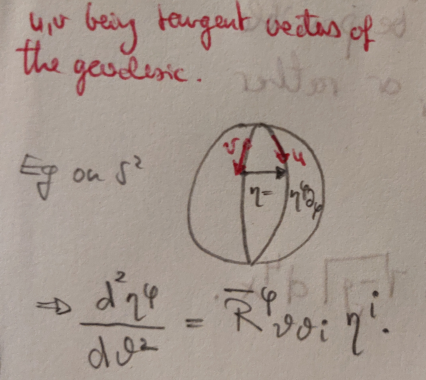
\includegraphics[width=0.7 \textwidth]{gfx/Geodesicdeviation.png}
\end{figure}
\begin{equation}
	\frac{\md ^2 \eta^{\varphi}}{\md \vartheta^2} = \bar{R}^{\varphi}_{\vartheta \vartheta i} \eta^i.
\end{equation}




\subsection{Equivalent treatment of Geodesic deviation - Caroll}
The defining property of Euclidean (flat) geometry is the parallel postulate: initially parallel lines remain
parallel forever. Of course in a curved space this is not true; on a sphere, certainly, initially
parallel geodesics will eventually cross. We would like to quantify this behavior for an
arbitrary curved space. The problem is that the notion of “parallel” does not extend naturally from flat to curved
spaces.\\
\\
Instead what we will do is to construct a one-parameter family of geodesics, $γ_s (t)$.
That is, for each $s \in \mR, γ$ is a geodesic parametrized by the affine parameter $t$. The
collection of these curves defines a smooth two-dimensional surface (embedded in a manifold
$M$ of arbitrary dimensionality). The coordinates on this surface may be chosen to be $s$ and
$t$, provided we have chosen a family of geodesics which do not cross. The entire surface is
the set of points $x^μ (s, t) \in M$. We have two natural vector fields: the tangent vectors to the
geodesics
\begin{equation}
T^\mu = \frac{\partial x^\mu}{\partial t},
\end{equation}
and the deviation vectors
\begin{equation}
S^\mu = \frac{\partial x^\mu}{\partial s}.
\end{equation}
This name derives from the informal notion that $S^μ$ points from one geodesic towards the
neighbouring ones.\\
The idea that $S^\mu$ points from one geodesic to the next inspires us to define the “relative
velocity of geodesics,”
\begin{equation}
V^\mu = (\nabla_T S)^\mu = T^\rho \nabla_\rho S^\mu
\end{equation}
and the “relative acceleration of geodesics,”
\begin{equation}
a^\mu =  (\nabla_T V)^\mu = T^\rho \nabla_\rho V^\mu.
\end{equation}
You should take the names with a grain of salt, but these vectors are certainly well-defined.\\
One finds
\begin{mybox}{Equation of geodesic deviation}
	\begin{equation}
	a^\mu = \nabla^2_{\dot{\gamma}(t)} S^\mu= \bar{R}^\mu_{\rho \sigma \nu} T^\nu T^\rho S^\sigma
	\end{equation}
	It expresses something that we might have
	expected: the relative acceleration between two neighbouring geodesics is proportional to the
	curvature.
	Physically, of course, the acceleration of neighbouring geodesics is interpreted as a manifestation of gravitational tidal forces..
\end{mybox}
















\newpage
\section{Einstein's field equations}
The field equations for gravitation are inevitably going to be more complicated than those for electromagnetism. Maxwell's equations are linear because the electromagnetic field does not itself carry charge, whereas gravitational fields do carry energy and momentum and must therefore contribute to their own source. Thus, the gravitational field equations will have to be non-linear partial differential equations, the non-linearity representing the effect of gravitation on itself.
\subsection{A not successful attempt via Poisson's equation}
Poisson’s equation can be made relativistically invariant by substituting it by
\begin{equation}
\label{eq:failedattemptEinstein}
	c^{-2} \square  \Phi = 4 \pi \mG T^\mu_\mu.
\end{equation}
In the limit of weak fields and
non-relativistic matter, this reduces to Poisson’s equation
\begin{equation}
	\Delta \Phi = 4 \pi \mG \rho.
\end{equation}
since then the time derivative in d’Alembert’s operator and the pressure contributions to T can
be neglected.\\
Why is this a problematic approach ?\\
First, the equivalence principle implies a gravitational redshift, which has been demonstrated
experimentally. One must thus require from a theory of gravity that it does lead to gravitational
redshift. However, in a theory with a Minkowskian metric, the emitted photons in an elevator,
which is at rest in a gravitational field, will propagate to the receiver at the ceiling along world
lines which may be curved, but must be parallel because the metric is constant. Hence there
cannot be gravitational redshift in a theory of gravity in flat space-time.
Second, \ref{eq:failedattemptEinstein} is a linear equation. However, there is also energy contained in the gravitational
field, which should be a source for gravity itself. So the gravitational theory cannot be linear.
Third, the gravitational potential of the Sun should be static so that the time derivative in
d’Alembert’s operator vanishes. This yields an equation which is almost identical to Poisson’s
equation except for the extra pressure contribution due to the trace of the energy-momentum
tensor on the right-hand side. Clearly, this does not give rise to a perihelion shift, which is
observed for Mercury so that the theory contradicts observations.
\\
\\
Starting off with a scalar theory of gravity, ie. one starts with the Lagrangian of a free particle in Special Relativity and multiplies it with the
factor $1 + \phi/c^2$ since this is the only possible Lagrangian that yields the right weak-field (Newtonian)
limit, one finds a perihelion shift a sixth of the actual value and with wrong sign.










\subsection{Heuristic Derivation}
In dealing with these non-linear effect we are guided once again by the Principle of Equivalence. At any point $X$ in an arbitrarily strong gravitational field, we can define a locally inertial coordinate system such that
\begin{equation}
	g\munu(X) = \eta\munu, \qquad \left(\frac{\partial g\munu(X)}{\partial x^\gamma}\right)_{x=X} =0.
\end{equation}
Hence for $x$ near $X$, the metric tensor $g\munu$ can differ from $\eta\munu$ only by terms quadratic in $x-X$. In this coordinate system the gravitational field is weak near $X$, and we can hope to describe the field by \emph{linear} partial differential equations. And once we know what these weak-field equations are, we can find the general field equations by reversing the coordinate transformation that made the field weak.\\
In the weak field limit, we have $\rho \approx T_{00}, g_{00} \approx -(1+2 \phi)$, such that the Poisson equation becomes
\begin{equation}
	\nabla^2 g_{00} = - 8 \pi \mG T_{00}.
\end{equation}
This field equation is only supposed to hold for weak static fields generated by nonrelativistic matter, and is not even Lorentz invariant as it stands. However, we can then guess 
\begin{equation}
	G_{\alpha \beta} = - 8 \pi \mG T_{\alpha \beta},
\end{equation}
where $G_{\alpha \beta}$ is a linear combination of the metric and its first and second derivatives. It follows from the principle of equivalence that the equations which govern gravitational fields of arbitrary strength must take the form
\begin{equation}
	G\munu = - 8 \pi \mG T\munu
\end{equation}
where $G\munu$ is a tensor which reduces to $G_{\alpha \beta}$ for weak fields. One can form a variety of tensors $G\munu$. In order to remove the ambiguity, we shall assume that the \emph{gravitational field equations are uniform in scale}, such that only the tensor containing $2$ derivative metric components are allowed, since the whole of $G\munu$ must have the dimensions of a second derivative. Combining all constrains one has on $G\munu$ (symmetry by symmetry of $T\munu$, conservation by conservation of $T\munu$, tensor, contains $2$ derivatives of the metric, weak field limit, Bianchi identity), one finds
\begin{equation}
	G\munu = R\munu -\half \mathcal{R}g\munu.
\end{equation}\\
\\
Without looking at failed attempts with only including $R_{\mu \nu}$ and $\nabla^2 g = 0$, one therefore finds:
\begin{equation}
	G_{\mu \nu} = \kappa T_{\mu \nu}.
\end{equation}
This equation satisfies all of the obvious requirements;
the right-hand side is a covariant expression, as required by general covariance, of the energy and momentum density in the form of a symmetric and conserved $(0, 2)$ tensor, as required by energy-momentum conservation, while the left-hand side is a symmetric and
conserved $(0, 2)$ tensor constructed from the metric, which replaces the gravitational potential, and its first and second derivatives. It
only remains to see whether it actually reproduces gravity as we know it.
With the normalization fixed by comparison
with the Newtonian limit, we can present Einstein’s equations for general relativity:
\begin{equation}
	R_{\mu \nu} - \frac{\mathcal{R}}{2} g_{ \mu \nu } = \frac{8 \pi \mathcal{G}}{c^4} T_{\mu \nu}.
\end{equation}
\marginpar{10 $2^{nd}$ order coupled, non-linear (since $G=G[g]$ and $T=T[g]$), partial differential equations for the metric.}
\begin{mybox}{Einstein's field equations}
	By heuristic derivation with $\Lambda=0$,
	\begin{equation}
	\label{eq:einsteinfieldeqs}
	G_{\mu \nu}=\frac{8 \pi \mathcal{G}}{c^4} T_{\mu \nu} \quad \Leftrightarrow \quad R_{\mu \nu}=\frac{8 \pi \mathcal{G}}{c^4} \left(T_{\mu \nu}-\frac{1}{2} g_{\mu \nu} \mathrm{Tr}T\right).
	\end{equation}
	Einstein's field equations are \emph{unique} as stated by Lovelock, i.e. $G$ must be of the form $G=\kappa T+\Lambda g$, with $\kappa$ and $\Lambda$ constants. The correct Newtonian limit then requires $\kappa = \frac{8 \pi \mathcal{G}}{c^4}$, and $\Lambda$ is the "cosmological constant".
	
\end{mybox}

In a vacuum $T\munu$ vanishes, such that the Einstein field equations in empty space are
\begin{equation}
	R\munu=0.
\end{equation}
In a space-time of two or three dimensions this would imply the vanishing of the full Riemann tensor $\bar{R}_{\mu \nu \lambda  \sigma}$, and the consequent absence of gravitational fields. It is only in four or more dimensions that true gravitational fields can exist in empty space.\\
\\
Note that in Steven Weinberg's Gravitation and Cosmology there is an alternative derivation of the Einstein field equations which is more general but very technical. It yields the insight that if we want a more general equation than Einstein's, which reduces in the weak-field limit to a second-order equation with $G_{\alpha \beta}$ on the LHS, then we must pay the price of allowing new elements unrelated to the metric tensor or its derivatives to enter, \emph{and} we must give up the possibility of deriving Newton's theory as a limiting case.
\subsubsection{On the uniqueness of Einstein's field equations via Lovelock}
Assuming that the gravitational field equations can be written in the form $D[g] = T$ , where $D[g]$
is a functional of the metric tensor $g$ and $T$ is the energy-momentum tensor, Lovelock’s theorem
states that $D[g]$ must be a linear combination of the Einstein and metric tensors, $D[g] = αG + βg$
if $D[g]$ depends on $g$ and its derivatives only up to second order. Thus, the field equations must
be of the form $G + βα^{ −1} g = α^{ −1} T$ or $G + Λg = κT$ . The correct Newtonian limit then requires
that $κ = 8π\mG c^{−4}$ , and $Λ$ is the cosmological constant.





\subsection{On the Meaning of the Field Equations}
These tell us how the curvature of spacetime reacts to the presence of energy-momentum.
Einstein’s equations may be thought of as second-order differential equations for the
metric tensor field $g_{μν}$ . There are ten independent equations (since both sides are symmetric
two-index tensors), which seems to be exactly right for the ten unknown functions of the
metric components. However, the Bianchi identity $∇_μ G^{μν} = 0$ represents four constraints on
the functions $R_{μν}$ , so there are only six truly independent equations in \ref{eq:einsteinfieldeqs}. In fact this is
appropriate, since if a metric is a solution to Einstein’s equation in one coordinate system $x^\mu$ it should also be a solution in any other coordinate system $x^{\mu^\prime}$. This means that there are
four unphysical degrees of freedom in $g_{μν}$ (represented by the four functions $x^{μ^\prime} (x^μ )$), and
we should expect that Einstein’s equations only constrain the six coordinate-independent
degrees of freedom.\\
\\
As differential equations, these are extremely complicated; the Ricci scalar and tensor are
contractions of the Riemann tensor, which involves derivatives and products of the Christoffel
symbols, which in turn involve the inverse metric and derivatives of the metric. Furthermore,
the energy-momentum tensor $T_{μν}$ will generally involve the metric as well. The equations
are also nonlinear, so that two known solutions cannot be superposed to find a third. It
is therefore very difficult to solve Einstein’s equations in any sort of generality, and it is
usually necessary to make some simplifying assumptions. Even in vacuum, where we set the
energy-momentum tensor to zero, the resulting equations
\begin{equation}
	R_{\mu \nu} = 0
\end{equation}
can be very difficult to solve. The most popular sort of simplifying assumption is that the
metric has a significant degree of symmetry, and we will talk later on about how symmetries
of the metric make life easier.
\\
\\
The nonlinearity of general relativity is worth remarking on. In Newtonian gravity the
potential due to two point masses is simply the sum of the potentials for each mass, but clearly this does not carry over to general relativity (outside the weak-field limit). There is
a physical reason for this, namely that in GR the gravitational field couples to itself. This
can be thought of as a consequence of the equivalence principle — if gravitation did not
couple to itself, a “gravitational atom” (two particles bound by their mutual gravitational
attraction) would have a different inertial mass (due to the negative binding energy) than
gravitational mass.
From a particle physics point of view this can be expressed in terms of
Feynman diagrams. The electromagnetic interaction between two electrons can be thought
of as due to exchange of a virtual photon:

\begin{figure}[h!]
	\centering
	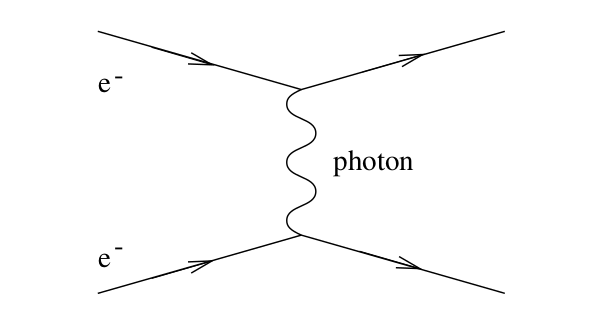
\includegraphics[width=0.7\linewidth]{gfx/QEDDiagram}
	\caption{}
	\label{fig:qeddiagram}
\end{figure}
But there is no diagram in which two photons exchange another photon between themselves;
electromagnetism is linear. The gravitational interaction, meanwhile, can be thought of
as due to exchange of a virtual graviton (a quantized perturbation of the metric). The
nonlinearity manifests itself as the fact that both electrons and gravitons (and anything
else) can exchange virtual gravitons, and therefore exert a gravitational force:

\begin{figure}[h!]
	\centering
	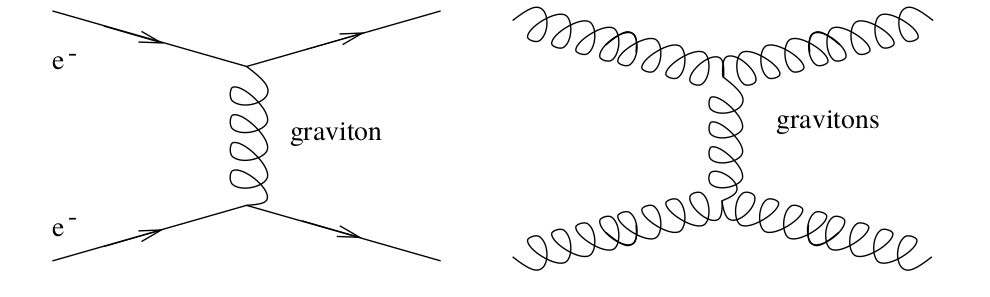
\includegraphics[width=0.7\linewidth]{gfx/GravityDiagram}
	\caption{}
	\label{fig:gravitydiagram}
\end{figure}

There is nothing profound about this feature of gravity; it is shared by most gauge theories,
such as quantum chromodynamics, the theory of the strong interactions. (Electromagnetism
is actually the exception; the linearity can be traced to the fact that the relevant gauge group,
$U(1)$, is abelian.) But it does represent a departure from the Newtonian theory.




































\newpage
\section{On the action principle - Weinberg}
There are a great many physical systems whose dynamic equations can be derived from a "principle of least action," that is, from a statement that some functional of the dynamical variables, the "action," is stationary w.r.t. small variations of these variables. This formulation of the dynamic equations has one great advantage: \emph{It allows us to establish an immediate connection between symmetry principles and conservation laws.}\\
The symmetry of the action that concerns us most in GR is general covariance. In the following, we shall develop a general definition of the energy-momentum tensor for any material system, as a functional derivative of the action for that system. The use of the action principle and general covariance will then allows us to show that this tensor is indeed conserved.\\
To achieve a truly general formulation of Gr i.t.o. an action principle, it is necessary to uncover a question that has been carefully buried until now: How can we incorporate the effects of gravitation into the field theories of particles with half-integer spin= The answer requires the tetrad formalism, which is based directly on the families of locally inertial frames.
\subsection{General definition of the Energy-Momentum-tensor by Weinberg}
We are going to define the energy-momentum tensor for a material system described by an action $S_M$ as the "functional derivative" of $S_M$ w.r.t. $g\munu$. That is, we imagine $g\munu(x)$ to be subject to an infinitesimal variation
\begin{equation}
	g\munu \rightarrow g\munu +  \delta g\munu
\end{equation}
where $\delta g\munu$ is arbitrary, except that it is required to vanish as $\abs{x^\lambda}\rightarrow\infty$. The action $S_M$ will not be stationary w.r.t. this variation, because for the moment we are regarding $g\munu(x)$ not as a dynamical variable like $x^\mu_n$ or $A_\mu$ but as an external field. Rather, $\delta S_M$ will be some linear functional of the infinitesimal $\delta g\munu(x)$, and therefore takes the form
\begin{mybox}{General definition of the energy-momentum tensor}
\begin{equation}
\label{eq:EnergyMomentumTensorWeinberg}
	\delta S_M = \half \int \md^4 x \sqrt{g(x)} T^{\mu \nu} (x) \delta g\munu(x).
\end{equation}
The coefficient $T^{\mu \nu}(x)$ is \textbf{defined} to be the energy-momentum tensor of this system. There exists a general proof that this $T^{\mu \nu}$ is a conserved symmetric tensor. 
\end{mybox}
This definition is closely analogous to a similar definition of the electric current $J^\mu$. We can break up the total matter action into a purely electromagnetic term $S_E$ and another term $S^\prime_M$ that describes the charged particles and their electromagnetic interactions
\begin{equation}
	S_M\equiv S_E+S^\prime_M \quad S_E \equiv -\frac{1}{4} \int \md^4 x \sqrt{g(x)} F\munu(x) F^{\mu \nu}(x).
\end{equation}
Consider the effect on $S^\prime_M$ of an infinitesimal variation in the vector potential $A_\mu \rightarrow A_\mu + \delta A_\mu$.
Since $S^\prime_M$ is not the whole action, the change in $S_M$ due to this variation in $A_\mu$ does not vanish, but it is necessarily a linear functional of $\delta A_\mu$:
\begin{mybox}{Definition of electromagnetic current}
	\begin{equation}
	\label{eq:electromagneticcurrent}
		\delta S^\prime_M = \int \md^4 x \sqrt{g(x)} J^\mu(x) \delta A_\mu(x)
	\end{equation}
	and the coefficient $J^\mu(x)$ is \textbf{defined} to be the electromagnetic current of the system.
\end{mybox}
\subsection{General Covariance and Energy-Momentum Conservation - Weinberg}
If the action $S_M$ for a material system is a scalar, then the statement that $\delta S_M$ vanishes is generally covariant, and also are the dynamical equations derived from this statement.\\
We shall therefore assume that $S_M$ is a scalar. This means that $S_M$ will be unchanged if we replace $x^\mu_n, A_\mu,g\munu$ by their primed values. If the original transformation $x^\mu\rightarrow x^{\prime \mu} $ was infinitesimal:
\begin{equation}
	x^{\prime \mu} = x^\mu + \epsilon^\mu(x)
\end{equation}
then the change in the dynamical variables is a change in 
\begin{align}
	\label{eq:variationalprincipleVariableChange}
\delta x^\mu_n(p) &= \epsilon^\mu(x_n(p)) \\
\delta A_\mu(x) &= -A_\nu(x) \frac{\partial \epsilon^\nu (x)}{\partial x^\mu} - \frac{\partial A_\mu(x)}{\partial x^\nu} \epsilon^\nu(x)\\
\delta g\munu(x) &= -g_{\mu \lambda} (x) \frac{\partial \epsilon^\lambda(x)}{\partial x^\nu} - g_{\lambda \nu} (x) \frac{\partial \epsilon^\lambda}{\partial x^\mu} - \frac{\partial g\munu(x)}{\partial x^\lambda} \epsilon^\lambda(x).
\end{align} 
The important point is that this is now an infinitesimal transformation of the dynamical variables alone, not of the coordinates over which we integrate, so the principle of stationary actions tells us that when the dynamical equations for $x^\mu_n$, $A_\mu$, and so on, are satisfied the change in these quantities produces no change in the matter action $S_M$. The only changes in $S_M$ comes from the variation in the external field $g\munu$, and \ref{eq:EnergyMomentumTensorWeinberg} gives for this change
\begin{equation}
	\delta S_M = - \half \int \md^4 x \sqrt{g} T^{\mu \nu} \left[g_{\mu \lambda} \frac{\partial \epsilon^\lambda}{\partial x^\nu} + g_{\lambda \nu} \frac{\partial \epsilon^\lambda}{\partial x^\mu} + \frac{\partial g\munu}{\partial x^\lambda} \epsilon^\lambda\right].
\end{equation}
If $S_M$ is a scalar, then this must vanish; integrating by parts gives then
\begin{equation}
	0 = \delta S_M=\int \md^4 x \epsilon^\lambda \left[ \frac{\partial}{\partial x^\nu} \left(\sqrt{g} T^\nu_\lambda\right)-\half \left(\frac{\partial g\munu}{\partial x^\lambda}\right)\sqrt{g} T^{\mu \nu}\right]
\end{equation}
and since $\epsilon^\lambda$ is arbitrary
\begin{equation}
	0 = \frac{\partial}{\partial x^\nu} \left(\sqrt{g} T^\nu_\lambda\right) - \half \left(\frac{\partial g\munu}{\partial x^\lambda}\right) \sqrt{g} T^{\mu \nu}
\end{equation}
or equivalently
\begin{mybox}{General Covariance implies Energy-momentum Conservation}
	\begin{equation}
		0= (T^\nu_\lambda)_{;\nu}.
	\end{equation}
	\textbf{Thus the energy-momentum tensor defined by Eq. \ref{eq:EnergyMomentumTensorWeinberg} is conserved (in the covariant sense) if and only if the matter action is a scalar}. Also, with $S_M$ a scalar, \ref{eq:EnergyMomentumTensorWeinberg} shows immediately that $T^{\mu \nu}$ is a symmetric \textbf{tensor}, so this definition of the energy-momentum tensor has all the properties for which one could wish.\\
	\textbf{This proof, that general covariance implies energy-momentum conservation, has an exact analogue in the proof that gauge invariance implies charge conservation}
\end{mybox}
The change in $S^\prime_M$ caused by an arbitrary gauge transformation can arise only form the change in $A_\mu$, since $S^\prime_M$ is stationary w.r.t. all other dynamical variables. A general infinitesimal gauge transformation $\epsilon$ will produce in $A_\mu$ the change $\delta A_\mu = \frac{\partial \epsilon}{\partial x^\mu}$. Inserting this in \ref{eq:electromagneticcurrent}, we see that $S^\prime_M$ is gauge invariant if and only if
\begin{equation}
0 = \delta S^\prime_M = \int \md^4 x \sqrt{g}J^\mu \frac{\partial \epsilon}{\partial x^\mu}.
\end{equation}
Integrating by parts gives
\begin{equation}
	0=\int \md^4 x \epsilon \frac{\partial}{\partial x^\mu} \left(\sqrt{g} J^\mu\right)
\end{equation}
or, since $\epsilon$ is arbitrary
\begin{equation}
	0=\frac{1}{\sqrt{g}} \frac{\partial}{\partial x^\mu} \sqrt{g} J^\mu = J^\mu_{;\mu},
\end{equation}
implying charge conservation. \\
\emph{We see again how closely analogous are gauge invariance and general covariance.}
\subsubsection{Applications of the general energy momentum tensor: Einstein's field equations and Contracted Bianchi identity}
So far, the gravitational field $g\munu$ has been an external field that could be prescribed at will . (Indeed, \ref{eq:EnergyMomentumTensorWeinberg} usually provides the most convenient definition of the energy-momentum tensor even in the absence of gravitation.) We will now give $g\munu$ equations of its own, by adding to the total action $S$ a purely gravitational term $S_G$:
\begin{equation}
	S=S_M+S_G,
\end{equation}
\begin{equation}
	S_G \equiv - \frac{1}{16 \pi \mG} \int \sqrt{g(x)} \mathcal{R}(x) \md^4 x.
\end{equation}
Clearly $S_G$ is a scalar, so this would be a good candidate for a theory of gravitation even if we had no experience with gravitational phenomena. The application to $S$ of the principle of stationary action does in fact yields the Einstein field equations. This is further explored below.\\
Another application of \ref{eq:EnergyMomentumTensorWeinberg} besides the derivation of the Einstein field equations is to use it to derive the contracted Bianchi identity. Since $S_G$ is a scalar it must be stationary wr.t. variation \ref{eq:variationalprincipleVariableChange} in $g\munu$. Repeating the reasoning that led before to general covariance implying energy-momentum conservation, we now find that
\begin{equation}
	\left[R^\nu_\lambda - \half \delta^\nu_\lambda \mathcal{R}\right]_{;\nu} = 0
\end{equation}
which we recognize as the contracted Bianchi identity.\\
This formalism suggests that Einstein's theory might be modified by adding to $\mathcal{R}$ in the Einstein-Hilbert action terms proportional to $\mathcal{R}^2,\mathcal{R}^3,\dots$. Such terms would only show up on a sufficiently small space-time scale.
















\newpage
\section{Derivation of Einstein's Field Equations from Least Action Principle}
\marginpar{Lorentz-covariance $\Rightarrow$ scalar $\Rightarrow$ $\mathcal{R}$. All $\mathcal{R}^n$ are allowed, but $n=1$ is the simplest.}
\marginpar{Introduce normal coordinates where $\Gamma=0$, then arrive at tensor equality ($\partial \rightarrow \nabla$) to have generality of frame again.}

Since we only apply the Principle of General Covariance on a small scale compared with the scale of the gravitational field, we usually expect that it is only $g\munu$ and its first derivatives that enter our generally covariant equations. \emph{This is precisely what we need to construct the Einstein-Hilbert action solely from the Ricci scalar, thus assume Principle of General Covariance and we can then postulate that the invariant scalar of the theory should only depend on the metric and its first derivatives.}
The Lagrange density is a tensor density, which can be written as $\sqrt{−g }$ times a scalar. What
scalars can we make out of the metric? Since we know that the metric can be set equal to
its canonical form and its first derivatives set to zero at any one point, any non-trivial scalar
must involve at least second derivatives of the metric. The Riemann tensor is of course
made from second derivatives of the metric, and we argued earlier that the only independent
scalar we could construct from the Riemann tensor was the Ricci scalar $\mathcal{R}$. What we did not
show, but is nevertheless true, is that any non-trivial tensor made from the metric and its
first and second derivatives can be expressed in terms of the metric and the Riemann tensor.
Therefore, the only independent scalar constructed from the metric, which is no higher than
second order in its derivatives, is the Ricci scalar. Hilbert figured that this was therefore the
simplest possible choice for a Lagrangian, and proposed
\begin{equation}
	S_{\mathrm{EH}} [g] = \int_{D\subset M} \mathcal{R}[g] \eta = \int_D \mathcal{R}[g] \sqrt{-g} \md^4 x.
\end{equation}
To repeat, the reasoning is:\\
What we want for the construction of our theory is not a tensor, but a completely invariant thing to put into the Lagrangian. (Instead, Einstein said that the Stress-Energy Tensor equals another tensor, which is derivable from the curvature tensor.) The least-action principle must involve an integral over all space, which must be completely invariant to transformations. The integrand must be a world scalar:
\begin{equation}
\int \md^4 x (Scalar) = (Scalar \, invariant).
\end{equation}
We get such a scalar via the Ricci scalar. Now, the volume integral of this scalar is not invariant, because the volume element is not a scalar, need to use canonical volume form thus to altogether arrive at the Einstein-Hilbert action for empty space. The remarkable uniqueness of $\mathcal{D}[g]$ shown by Lovelock indicates that a Lagrangian formulation of GR should be possible starting from a scalar constructed from $\mathcal{D}$, or rather $\mathrm{Tr}\mathcal{D} \propto \mathcal{R}$.\\\\
\\
The equations of motion should come from varying the action with respect to the metric. The fact that gravity is attractive for likes and unlikes is a property of the Lagrangian, so that if we change $S\rightarrow -S$, the force changes sign. Note that the sign of the coupling constant $e,g,\lambda$ makes no difference, since it appears as a square in any diagram which represents a correction to the energy. The sign of the Coulomb forces comes from the sign of the time components in the Lagrangian. For gravity waves, since we are contracting over two indices, the signs cancel out and we have attraction. In fact let us consider variations with respect to the inverse metric $g^{\mu \nu}$ , which are slightly
easier but give an equivalent set of equations. Using $\mathcal{R} = g^{μν} R_{μν}$ , in general we will have
\begin{align}
	\delta S &=  \int \md^n x \left[\sqrt{-g} g^{\mu \nu} \delta R_{\mu \nu} + \sqrt{-g} R_{\mu \nu} \delta g^{\mu \nu} + \mathcal{R} \delta \sqrt{-g})\right] \\
	&= (\delta S)_1 + (\delta S)_2 + (\delta S)_3 \nonumber.
\end{align}
The second term $(δS)_2$ is already in the form of some expression times $δg^{μν}$ ; let’s examine
the others more closely.\\
Recall that the Ricci tensor is the contraction of the Riemann tensor, which is given by
\begin{equation}
	R^\rho_{\mu \lambda \nu} = \partial_\lambda \Gamma^\lambda_{\nu \mu} + \Gamma^\rho_{\lambda \sigma}\Gamma^\sigma_{\nu\mu} - (\lambda \leftrightarrow \nu). 
\end{equation}
The variation of this with respect the metric can be found first varying the connection with
respect to the metric, and then substituting into this expression. Let us however consider arbitrary variations of the connection, by replacing
\begin{equation}
	\Gamma^\rho_{\mu \nu} \rightarrow\quad \Gamma^\rho_{\mu \nu} + \delta \Gamma^\rho_{\mu \nu}.
\end{equation}
The variation $δΓ^ρ_{νμ}$ is the difference of two connections, and therefore is itself a tensor. We
can thus take its covariant derivative,
\begin{equation}
∇_λ (δΓ^ρ{νμ} ) = ∂_λ (δΓ^\rho_{\nu μ} ) + Γ^ρ_{λσ} δΓ^σ_{νμ} − Γ^σ_{λν} δΓ^ρ_{σμ} − Γ^σ_{λμ} δΓ^ρ_{νσ} .
\end{equation}
Given this expression it is easy to show that
\begin{equation}
	δR^ρ_{μλν} = ∇_λ (δΓ^ρ_{νμ} ) − ∇_ν (δΓ^ρ_{λμ} ).
\end{equation}
Therefore
\begin{align}
	(\delta S)_1 &= \int \md^n x \sqrt{−g} g^{μν} \left[ ∇_λ (δΓ^λ_{νμ} ) − ∇_ν (δΓ^λ_{λμ} )	\right]		 \nonumber \\
	&= \int \md^n x \sqrt{−g} ∇_σ \left[g^{μσ} (δΓ^λ_{λμ} ) − g^{μν} (δΓ^σ_{μν} ) \right],
\end{align}
where we have used metric compatibility and relabelled some dummy indices. But now we
have the integral with respect to the natural volume element of the covariant divergence of
a vector; by Stokes’s theorem, this is equal to a boundary contribution at infinity which we
can set to zero by making the variation vanish at infinity. Therefore this term contributes nothing
to the total variation.\\
To make sense of the $(δS)_3$ term we need to use the following fact, true for any matrix
$M$:
\begin{equation}
	\tr(\ln(M)) = \ln(\det M).
\end{equation}
Here, $\ln M$ is defined by $\exp(\ln M) = M$. The variation of this identity yields
\begin{equation}
	\tr(M^{-1} \delta M) = \frac{1}{\det(M)} \delta\left(\det(M)\right).
\end{equation}
Here we have used the cyclic property of the trace to allow us to ignore the fact that $M^{−1}$
and $δM$ may not commute. Now we would like to apply this to the inverse metric, $M = g^{μν}$. Then $\det M = g^{−1}$ (where $g = \det g_{μν}$ ), and
\begin{equation}
	\delta(g^{-1}) = \frac{1}{g} g_{\mu \nu}\delta g^{\mu \nu}.
\end{equation}
Now we can just plug in
\begin{align*}
	\delta \sqrt{-g} &= \delta \left[(-g^{-1})^{-\half}\right] \\
	&=- \half ((-g^{-1})^{-3/2} ) \delta(- g^{-1})\\
	&= -\half \sqrt{-g} g_{\mu \nu} \delta g^{\mu \nu}.
\end{align*}
Altogether, we thus find
\begin{equation}
	\delta S = \int \md^n x \sqrt{-g}  \left[R_{\mu \nu} - \frac{\mathcal{R}}{2} g_{\mu \nu} \right]\delta g^{\mu \nu}.
\end{equation}
This should vanish for arbitrary variations, so we are led to Einstein’s equations in vacuum:
\begin{equation}
	\frac{1}{\sqrt{-g}} \frac{\delta S}{\delta g^{\mu \nu}} = G_{\mu \nu} =0.
\end{equation}
What we would really like, however, is to get the non-vacuum field equations
as well. That means we consider an action of the form
\begin{equation}
	S = \frac{c^4}{8 \pi \mathcal{G}} S_{EH} + S_M
\end{equation}
where $S_M$ is the action for matter, and we have presciently normalized the gravitational
action. Following through the same procedure as above yields:
\begin{equation}
		\frac{1}{\sqrt{-g}} \frac{\delta S}{\delta g^{\mu \nu}} = \frac{c^4}{8 \pi \mathcal{G}} G_{\mu \nu} + \frac{1}{\sqrt{-g}} \frac{\delta S_M}{\delta g^{\mu \nu}},
\end{equation}
and we recover Einstein’s equations if we can set
\begin{equation}
\label{eq:GRenergymomentumtensor}
	T_{\mu \nu} = - \frac{2}{\sqrt{-g}} \frac{\delta S_M}{\delta g^{\mu \nu}}.
\end{equation}
What makes us think that we can make such an identification? In fact \ref{eq:GRenergymomentumtensor} turns out to
be the best way to define a symmetric energy-momentum tensor. The tricky part is to show
that it is conserved, which is in fact automatically true, but which we will not justify until
the next section.
\subsubsection{On the definition of energy-momentum tensors}
We say that \ref{eq:GRenergymomentumtensor} provides the “best” definition of the energy-momentum tensor because
it is not the only one you will find. In flat Minkowski space, there is an alternative definition which is sometimes given in books on electromagnetism or field theory. In this context energy-momentum conservation arises as a consequence of symmetry of the Lagrangian under spacetime translations. Noether’s theorem states that every symmetry of a Lagrangian
implies the existence of a conservation law; invariance under the four spacetime translations
leads to a tensor $S_{μν}$ which obeys $∂^\mu S_{μν} = 0$ (four relations, one for each value of $ν$). Applying Noether’s
procedure to a Lagrangian which depends on some fields $ψ^i$ and their first derivatives $∂_μ ψ^i$ ,
we obtain
\begin{equation}
\label{eq:canonicalenergymomentumtensor}
	S_{μν} =\sum_i \frac{\delta \mL}{\delta (\partial_\mu \psi^i)} ∂_ν ψ^i − η_{μν} \mL.
\end{equation}
You can check that this tensor is conserved by virtue of the
equations of motion of the matter fields. $S_{μν}$ often goes by the name “\emph{canonical energy-momentum tensor}”; however, there are a number of reasons why it is more convenient for
us to use \ref{eq:GRenergymomentumtensor}.
\begin{enumerate}
	\item \ref{eq:GRenergymomentumtensor} is in fact what appears on the right hand side of
	Einstein’s equations when they are derived from an action, and it is not always possible to
	generalize \ref{eq:canonicalenergymomentumtensor} to curved spacetime.
	\item But even in flat space \ref{eq:GRenergymomentumtensor} has its advantages; it is
	manifestly symmetric, and also guaranteed to be gauge invariant, neither of which is true for
	\ref{eq:canonicalenergymomentumtensor}.\\
	Since the Lagrangian changes if the gauge is changed, the canonical energy-momentum tensor (from SR) is not gauge invariant. This is a reflection of the non-localizability of the gravitational energy. Even in the linearised theory, it is not possible to find gauge invariant expressions for the energy and momentum densities.
\end{enumerate}
Note also that the canonical energy momentum tensor can be viewed as a generalization of the prescription to obtain the Hamiltonian, i.e. the energy, of a system from the corresponding Lagrangian via a Legendre transformation. Note further that the canonical energy-momentum tensor is not generally symmetric, the resulting theory is pathological ( there is no way to define angular momentum in the field for example). One can in fact add the Belinfante-Rosenfeld tensor to the canonical energy-momentum tensor in order to obtain a symmetric and conserved energy momentum tensor. Thus we see that corrections to the canonical Noether tensor that appear in the Belinfante-Rosenfeld tensor occur because we need to simultaneously vary the vierbein and the spin connection if we are to preserve local Lorentz invariance, c.f. BR tensor on Wikipedia.
\begin{mybox}{Weak Energy condition}
	Our real concern is with the
	existence of solutions to Einstein’s equations in the presence of “realistic” sources of energy
	and momentum, whatever that means. The most common property that is demanded of
	$T_{μν}$ is that it represent positive energy densities — no negative masses are allowed. In a
	locally inertial frame this requirement can be stated as $ρ = T_{00} ≥ 0$. To turn this into a coordinate-independent statement, we ask that
	\begin{equation}
	T_{\mu \nu} V^{\mu} V^{\nu} \geq 0 \quad \forall \; \mathrm{time-like} \; V^\mu
	\end{equation}
	This is known as the \emph{Weak Energy Condition}, or WEC.
\end{mybox}
Unfortunately it is not set in stone; indeed, it is straightforward to invent
otherwise respectable classical field theories which violate the WEC, and almost impossible
to invent a quantum field theory which obeys it. Nevertheless, it is legitimate to assume
that the WEC holds in all but the most extreme conditions.

\subsubsection{The trace of the energy-momentum tensor}
Consider a conformal transformation of the metric
\begin{equation}
	g^{\mu \nu}(x) \rightarrow e^{\lambda(x)} g^{\mu \nu}(x) \approx g^{\mu \nu} + \underbrace{\delta g^{\mu \nu}}_{\lambda g^{\mu\nu}}.
\end{equation}
With the definition of the energy momentum tensor
\begin{equation}
	T\munu = -  \frac{1}{\sqrt{-g}} \frac{\delta S}{\delta g\munu}
\end{equation}
we find for the variation of the action
\begin{align}
	\delta S &= \int \md^4 x \sqrt{-g} \frac{\delta S}{\delta g_{\mu \nu}} \delta g_{\mu \nu} \\
	&= - \int \md^4 x \sqrt{-g}^2 T^{\mu \nu} \lambda g\munu \\
	&= -\int \md^4 x \sqrt{-g}^2 \lambda T^\mu_\mu \\
	T^\mu_\mu = 0 \quad &\Rightarrow \delta S =
\end{align}
under conformal transformation. Thus, if the energy-momentum tensor has a vanishing trace, then it is
scale-invariant (under conformal transformation). Therefore, the corresponding theory is scale-invariant.



\subsection{The full Einstein field equations}
We have now justified Einstein’s equations in two different ways: as the natural covariant
generalization of Poisson’s equation for the Newtonian gravitational potential, and as the
result of varying the simplest possible action we could invent for the metric.\\
\\
\begin{mybox}{Einstein's field equations including $\Lambda$}
A constant
does not by itself lead to very interesting dynamics, it has an important effect if we add it
to the conventional Hilbert action. We therefore consider an action given by
\begin{equation}
	S =  \int_D \left(\mathcal{R}+2 \Lambda\right) \eta,
\end{equation}
\emph{Einstein's vacuum equations}, 
\begin{equation}
	G - \Lambda g=0,
\end{equation}
\end{mybox}
\marginpar{Variation is performed w.r.t $g$, later also $\delta g$, since $\delta \psi$ yields \emph{matter field equations}. This is frame independent since $\delta \mathcal{J}$ as $\mathcal{J}[g] = \mathcal{J}$.}
The complete equations are obtained by coupling gravity/geometry and matter.\\
Ignored possible boundary since $\delta g$ only inside $D$, include Gibbons-Hawking-York boundary term for manifold with boundary.\\
For $\Lambda$ on the RHS, $Λ$ can be interpreted as the “energy density of the vacuum,”
a source of energy and momentum that is present even in the absence of matter fields. This
interpretation is important because quantum field theory predicts that the vacuum should
have some sort of energy and momentum. In ordinary quantum mechanics, an harmonic
oscillator with frequency $ω$ and minimum classical energy $E_0 = 0$ upon quantization has a
ground state with energy $E_0 = \half h̄ω$. A quantized field can be thought of as a collection of
an infinite number of harmonic oscillators, and each mode contributes to the ground state
energy. The result is of course infinite, and must be appropriately regularized, for example 
by introducing a cut-off at high frequencies. The final vacuum energy, which is the regularized
sum of the energies of the ground state oscillations of all the fields of the theory, has no good
reason to be zero and in fact would be expected to have a natural scale $\Lambda \propto M^4_{pl}$, here the Planck mass is approximately $10^{19} GeV$, or $10^{−5} grams$. Observations of the
universe on large scales allow us to constrain the actual value of $Λ$, which turns out to be
smaller than $M^4_{pl}$ by at least a factor of $10^{120}$ . This is the largest known discrepancy between
theoretical estimate and observational constraint in physics, and convinces many people that
the “cosmological constant problem” is one of the most important unsolved problems today.
On the other hand the observations do not tell us that $Λ$ is strictly zero, and in fact allow
values that can have important consequences for the evolution of the universe. This mistake
of Einstein’s therefore continues to bedevil both physicists, who would like to understand
why it is so small, and astronomers, who would like to determine whether it is really small
enough to be ignored.

\subsubsection{This is how we use diffeomorphism invariance to postulate Einstein-Hilbert action}
We choose the action for the gravitational field to be
\begin{equation}
S_g = -\frac{1}{2 \lambda^2} \int \md^4x \mathcal{R}\sqrt{-g}.
\end{equation}
The curvature tensor appears when we take the variation of $S_g$ w.r.t. $g\munu$
\begin{equation}
\frac{\delta S_g}{\delta g\munu} = \frac{1}{2 \lambda^2} \sqrt{-g} \left(R^{\mu \nu} - \half \mathcal{R} g^{\mu \nu}\right).
\end{equation}
It is because of this that we can use the integral of $\mathcal{R}$ as the action of the gravitational part of the complete problem.
That because this stress tensor appears in this way, from a variational principle, its covariant divergence is neccessarily zero. We have seen the connection from the other direction-that we could deduce a variational principle provided that we started from a divergenceless tensor. \\
We want to show that if the functional 
\begin{equation}
S_g = \int \md^4 x \Sigma[g\munu]
\end{equation}
is invariant under coordinate transformations, then the covariant divergence of the variation of $S_g$ w.r.t. $g\munu$ is identically zero. Under the infinitesimal transformation to primed coordinates
\begin{equation}
x^\mu = x^{\mu^\prime} + h^\mu(x^\prime),
\end{equation}
the functional changes as, dropping primes on integration variables
\begin{equation}
S_g = \int \md^4 x \Sigma[g^\prime\munu] = \int \md^4 x \Sigma[g\munu] + \int \md^4x \frac{\delta \Sigma}{\delta g\munu} (h^\alpha_{,\nu} g_{\mu \alpha} + h^\alpha_{,\mu} g_{\nu \alpha} + h^\alpha g_{\mu \nu,\alpha} ).
\end{equation}
When we do an integration by parts on the second term of this expression, we convert it to an expression involving the functional derivatives of the function $\Sigma$. We it it equal to zero, since we know that the change in the action must be zero for any $h^\alpha$, because of the character of $\Sigma$.
\begin{equation}
\label{eq:Feynman1}
\frac{\partial}{\partial x^\mu} \left[\frac{\delta \Sigma}{\delta g\munu} g_{\nu \alpha}\right] - \half \frac{\delta \Sigma}{\delta g\munu} \frac{\partial g\munu}{\partial x^\alpha} = 0.
\end{equation}
Let us denote by $\mG^{\mu \nu}$ the variation of $2 \lambda^2 S_g$ w.r.t. $g\munu$:
\begin{equation}
\mG^{\mu \nu} = 2 \lambda^2 \frac{\delta Ŝ_g}{\delta g\munu}.
\end{equation}
This quantitiy is a contravariant tensor density of second rank, thus \ref{eq:Feynman1} becomes
\begin{equation}
(g_{\alpha\mu} \mG^{\mu \nu})_{,\nu} - \half g_{\mu \nu,\alpha} \mG^{\mu \nu} =,
\end{equation}
which is equivalent to the statement that the covariant divergence of $\mG^{\mu \nu}$ iszero:
\begin{equation}
\label{eq:Feynman2}
\mG^{\mu \nu}_{;\nu} = 0.
\end{equation}
Using tensor and covariant derivative formulae as written above, it is quite straightforward to deduce that \ref{eq:Feynman1} and \ref{eq:Feynman2} are equivalent. Thus, we see that the invariance of an action results in the  construction of a \emph{tensor density} which is automatically divergenceless. The tensor associated with the tensor density $\mG^{\mu \nu}$  is also divergenceless
\begin{equation}
G^{\mu \nu} = \mG^{\mu \nu} / \sqrt{-g}, \quad G^{\mu \nu}_{;\nu} =0.
\end{equation}



\subsection{Coordinate Conditions - A note on gauge freedom in Einstein's field equations -Weinberg}
\label{subsec:gaugefreedomGR}
The symmetric tensor $G\munu$ has $10$ independent components, so Einstein's field equations comprise $10$ algebraically independent equations. The unknown metric tensor also has $10$ algebraically independent components, and at first sight one would think that Einstein equations (with appropriate boundary conditions) would suffice to determine the $g\munu$ uniquely. However, this is not so. Although algebraically independent, the $10\, G\munu$ are related by four differential identities, the Bianchi identities:
\begin{equation}
G^\mu_{\nu ; \mu} = 0,
\end{equation}
which are a \emph{reduction of equations (Gauge freedom)}. Thus there are not $10$ functionally independent equations, but only $10-4=6$, leaving us with four degrees of freedom in the $10$ unknowns $g\munu$. These degrees of freedom correspond to the fact that if $g\munu$ is a solution of Einstein's equation, then so is $g^\prime\munu$, where $g^\prime\munu$ is determined from $g\munu$ by a general coordinate transformation $x\rightarrow x^\prime$. Such a coordinate transformation involves four arbitrary functions $x^{\mu^\prime} (x)$, giving to the solutions of the field equations \ref{eq:einsteinfieldeqs} just four degrees of freedom.\\
\subsubsection{Comparison with gauge freedom in EM}
The failure of Einstein's equations to determine $g\munu$ uniquely is closely analogous with the failure of Maxwell's equations to determine the vector potential $A_\mu$ uniquely, hence these redundancies in the degrees of freedom are a \emph{gauge freedom}. When written i.t.o. the vector potential, Maxwell's equations read
\begin{equation}
\label{eq:eomVectorPotentialEM}
\square A_\alpha - \frac{\partial^2}{\partial x^\alpha \partial x^\beta} A^\beta = - J_\alpha.
\end{equation}
There are four equations for the four unknowns, but they do no determine $A_\alpha$ uniquely, because the LHS of these equations are related by a differential identity analogous to the Bianchi identity
\begin{equation}
\frac{\partial}{\partial x^\alpha} \left[\square A^\alpha - \frac{\partial^2}{\partial x_\alpha \partial x^\beta} A^\beta \right] \equiv 0.
\end{equation}
Thus the number of functionally independent equations is really only $4-1=3$, and there is one degree of freedom in the solution of the four $A_\alpha$. This degree of freedom of course corresponds to \emph{gauge invariance}; given any solution $A_\alpha$, we can find another solution $A^\prime_\alpha \equiv A_\alpha + \frac{\partial \Lambda}{\partial x^\alpha}$, with $\Lambda$ arbitrary.\\
The ambiguity in the solutions of Maxwell's and Einstein's equations can be removed by main force. In the case of Maxwell's equation we do this by choosing a particular gauge. For instance, given any solution $A_\alpha$, we can always construct a solution $A^\prime_\alpha$ such that
\begin{equation}
\label{eq:LorentzGaugeEM}
\partial_\alpha A^{\prime \alpha} =0
\end{equation} 
by setting
\begin{equation}
A^\prime_\alpha \equiv A_\alpha + \frac{\partial \Phi}{\partial x^\alpha}
\end{equation}
where $\Phi$ is defined by
\begin{equation}
\square\Phi = - \frac{\partial A^\alpha}{ \partial x^\alpha}.
\end{equation}
Such a solution is said to be in the \emph{Lorentz gauge}.\\
The condition \ref{eq:LorentzGaugeEM} when added to the \emph{three} independent equations \ref{eq:eomVectorPotentialEM} completes a system of four equations that, with appropriate boundary conditions, will generally determine the four $A_\alpha$ uniquely.
\subsubsection{Adopt the same philosophy for the gauge freedom in GR}
In the same ways, we can eliminate the ambiguity in the metric tensor by adopting some particular coordinate system(i.e. the redundancy of coordinate systems is the gauge freedom in GR). The choice of a coordinate system can be expressed in four \emph{coordinate conditions}, which, when added to the six independent Einstein equations, determine an unambiguous solution.\\
\begin{mybox}{Harmonic coordinate condition}
	One particular convenient choice of a coordinate system is represented in the \emph{harmonic coordinate conditions}
	\begin{equation}
	\label{eq:harmoniccoordinatecondition}
	\Gamma^\lambda \equiv g^{\mu \nu} \Gamma^\lambda\munu =0.
	\end{equation}
	It is always possible to choose a coordinate system in which this holds, since, if $\Gamma^\rho$ does not vanish, we can always define a new coordinate system $x^{\prime \lambda}$ by solving the second-order partial differential equations
	\begin{equation}
	g^{\rho \sigma} \frac{\partial^2 x^{\prime \lambda}}{\partial x^\rho \partial x^\sigma} = \frac{\partial x^{\prime \lambda}}{\partial x^\rho} \Gamma^\rho
	\end{equation}
	and contracting \ref{eq:christoffelTrafo} to the form $\Gamma^{\prime \lambda} =..$ then yields $\Gamma^{\prime \lambda}=0$ in the $x^\prime$-system.
\end{mybox}
The four conditions \ref{eq:harmoniccoordinatecondition} are of course not generally covariant, since their purpose is to remove the ambiguity in the metric tensor owing to the general covariance of the Einstein equations.
\begin{mybox}{Equivalent form of the harmonic coordinate condition}
	With the contracted Christoffel i.t.o. the metric tensor, one finds
	\begin{equation}
	\label{eq:harmoniccoordinateconditionEquivalent}
	\frac{\partial}{\partial x^\kappa} \left(\sqrt{g} g^{\lambda \kappa}\right)=0.
	\end{equation}
\end{mybox}
\begin{mybox}{Harmonic coordinates definition}
	We are now in a position to explain the term "harmonic coordinates". A function $\phi$ is said to be harmonic if $\square^2 \phi$ vanishes,
	where $\square^2$ is the \emph{invariant} or \emph{covariant d'Alembertian}
	\begin{equation}
	\square^2 \phi \equiv \left(g^{\lambda \kappa} \phi_{;\lambda} \right)_{;\kappa} = g^{\lambda \kappa} \frac{\partial^2 \phi}{\partial x^\lambda \partial x^\kappa} - \Gamma^\lambda \frac{\partial \phi}{\partial x^\lambda}.
	\end{equation}
\end{mybox}
\begin{mybox}{"Harmonic Gauge" - harmonic coordinate condition in $x^\mu$}
	If $\Gamma^\lambda=0$ then the coordinates are themselves harmonic functions,
	\begin{equation}
	\label{eq:harmonicCoordinatesGauge}
	\square^2 x^\mu = 0
	\end{equation}
	thus justifying our application of the adjective "harmonic" to such coordinate systems.
\end{mybox}
In the absence of gravitational fields, the obvious harmonic coordinate system is that of Minkowski, in which $g^{\lambda \kappa} = \eta^{\lambda \kappa}$ and $g=1$, so that \ref{eq:harmoniccoordinateconditionEquivalent} is satisfied trivially. In the presence of weak gravitational fields the harmonic coordinate systems may be pictured as nearly Minkowskian. Another related advantage of the harmonic coordinate condition is that, as shown later on, its use produces a very great simplification in the weak-field equations, similar to the simplification brought to Maxwell's equations by use of the Lorentz gauge, c.f. Weak field treatment in \ref{ch:GRapplications}.








\section{The energy-momentum tensor}
\subsection{Energy, Momentum, and Angular Momentum of Gravitation - Weinberg}
Similar to the linear gravity analysis in \ref{ch:GRapplications}, we adopt here a coordinate system that is quasi-Minkowskian, in the sense that the metric $g\munu$ approaches the Minkowski metric $\eta\munu$ at great distances from the finite matter system under study. (This is the case in harmonic coordinate systems, and others as well.) We then write
\begin{equation}
	g\munu = \eta\munu + h\munu
\end{equation}
so that $h\munu$ vanishes at infinity. (However, $h\munu$ is not assumed to be small everywhere.)  The part of the Ricci tensor linear in $h\munu$ is then
\begin{equation}
R^{(1)}_{\mu \kappa} \equiv \half \left[\frac{\partial^2 h^\lambda_\lambda}{\partial x^\mu \partial x^\kappa} - \frac{\partial^2 h^\lambda_\mu}{\partial x^\lambda \partial x^\kappa } - \frac{\partial^2 h^\lambda_\kappa }{\partial x^\lambda \partial x^\mu} + \frac{\partial^2 h_{\mu \kappa}}{\partial x^\lambda \partial x_\lambda}\right].
\end{equation}
We are adopting the convenient convention that indices on $h\munu, R^{(1)}\munu$, and $\partial/\partial x^\lambda$ are raised and lowered with $\eta$s, for example, $h^\lambda_\lambda \equiv \eta^{\lambda \nu} h_{\lambda \nu}$ and $\partial/\partial x_\lambda \equiv \eta^{\lambda \nu} \partial/\partial x^\nu$, whereas indices on true tensors such as $R\munu$ are raises and lowered with $g$s as usual. 
\begin{mybox}{Energy-momentum tensor of gravity}
	The exact Einstein equations linearized in the perturbation can then be written as
	\begin{equation}
	\label{eq:linearizedEinstein}
	R^{(1)}_{\mu \kappa} - \half \eta_{\mu \kappa} R^{(1)\lambda}_\lambda = - 8 \pi \mG \left[T_{\mu \kappa} + t_{\mu \kappa} \right]
	\end{equation}
	where
	\begin{equation}
		\label{eq:energymomentumtensorofGravity}
		t_{\mu \kappa} \equiv \frac{1}{8 \pi \mG} \left[R_{\mu \kappa} - \half g_{\mu \kappa} R^\lambda_\lambda - R^{(1)}_{\mu \kappa} + \half \eta_{\mu \kappa} R^{(1)\lambda}_\lambda\right].
	\end{equation}
	Equation \ref{eq:linearizedEinstein} has just the form we should expect for the wave equation of a field of spin $2$  but with the peculiarity that its "source" $T\munu+t\munu$ depends explicitly on the field $h\munu$. We interpret this feature by saying that the field $h\munu$ is generated by the total densities and fluxes of energy and momentum, and 
	\textbf{$t\munu$ is simply the energy-momentum "tensor" of the gravitational field itself}. \\
		\end{mybox}
	\begin{mybox}{Energy-momentum tensor of matter and gravitation}
		That is, we interpret the quantity
		\begin{equation}
		\label{eq:totalenergymomentumtensorGravityAndMatter}
			\tau^{\nu \lambda} \equiv \eta^{\nu \mu} \eta^{\lambda \kappa} \left[T_{\mu \kappa} + t_{\mu \kappa}\right]
		\end{equation}
		as the total energy-momentum "tensor" of matter \textbf{and} gravitation. 
\end{mybox}
There are several properties of $\tau^{\nu \lambda}$ that support this interpretation:
\begin{enumerate}
	\item The linearized Ricci tensor obey the linearized Bianchi identities, such that via the field equations $\tau^{\nu \lambda}$ is locally conserved
	\begin{equation}
		\frac{\partial}{\partial x^\nu} \tau^{\nu \lambda} = 0.
	\end{equation}
	Note that although $T^{\nu \lambda}$ obeys the covariant conservation law $T^{\nu \lambda}_{;\nu}=0$, which really describes the \emph{exchange} of energy between matter and gravitation; the quantity $\tau^{\nu \lambda}$ is conserved in the ordinary sense. It follows that
	\begin{equation}
		P^\lambda \equiv \int_V \tau^{0 \lambda} \md^3 x
	\end{equation}
	may be interpreted as the total-energy momentum "vector" of the system, including matter, electromagnetism, \textbf{and} gravitation; $\tau^{i \lambda}$ is the corresponding flux.
	\item Besides being conserved, $\tau^{\nu \lambda}$ is also symmetric, implying that $M^{\mu \nu \lambda} \equiv \tau^{\mu \lambda} x^\nu - \tau^{\mu \nu} x^\lambda$ suffices
	\begin{equation}
		\frac{\partial}{\partial x^\mu} M^{\mu \nu \lambda} = 0.
	\end{equation}
	We can thus interpret $M^{0\nu\lambda}$ and $M^{i \nu \lambda}$ as the density and flux of the total angular momentum
	\begin{equation}
		J^{\nu \lambda} \equiv \int \md^3 x \; M^{0 \nu \lambda} = - J^{\lambda \nu}
	\end{equation}
	that is constant if $M^{i \nu \lambda}$ vanishes on the surface of the volume of integration.
	\item We can compute $t_{\mu \kappa}$ as a power series in $h$, and find that the first term is \emph{quadratic}.\\
	The example of electrodynamics would have led us to expect the energy-momentum "tensor" of gravitation to start with a term quadratic in $h\munu$.  The presence in $t\munu$ of terms of third and higher order imply means that the gravitational interaction of the gravitational field with itself also contributes to the total energy and momentum. Of course, when the gravitational field is weak, $h\munu$ is small, so our inclusion of $t_{\lambda \nu}$ in \ref{eq:totalenergymomentumtensorGravityAndMatter} (and our use of $\eta$ to raise indices) does no seriously change our picture of the energy-momentum content of physical systems.
	\item Though not generally covariant, $t\munu, \tau^{\nu \lambda},$ and $M^{\mu \nu \lambda}$ are at least Lorentz-covariant. Thus for a closed system $P^\lambda$ and $J^{\nu \lambda}$ are not only constant, but also Lorentz-covariant.
	\item We chose at the beginning of this section to work in a coordinate system in which $\munu$ vanishes at infinity. Far away from the finite material system that produces the gravitational field, $T\munu$ is zero and $t\munu$ is of order $h^2$, so the source term on the RHS of the field equations \ref{eq:linearizedEinstein} is effectively confined to a finite region. This suggests that in a large variety of physical problems $h\munu$ will behave at great distances as do the potentials in electrostatics or Newtonian gravitational theory, that is, for $r\rightarrow\infty$:
	\begin{equation}
		h\munu= \mathcal{O}(r^{-1}), \; \frac{\partial h\munu}{\partial x^\lambda} = \mathcal{O}(r^{-2}), \; \frac{\partial^2 h\munu}{\partial x^\lambda \partial x^\rho} = \mathcal{O}(r^{-2})\; \Rightarrow\; t\munu = \mathcal{O}(r^{-4})
	\end{equation}
	so the integral $\int \tau^{0 \lambda} \md^3 x$ that gives the total energy and momentum \emph{converges}. This is why it was so important to identify the coordinate system as quasi-Minkowskian; if $g\munu$ approached the metric of spherical polar coordinates at infinity, then our definitions would have led to a gravitational energy density concentrated at infinity! Note that the asymptotic behaviour $h\munu$ as above is not always valid. If the system is eternally radiating gravitational waves, then $h\munu$ oscillates such that its derivatives are of same order, giving an infinite total energy, which is what we would expect for gravitational radiation filling all of space.
	\item By its construction, $\tau^{\nu \lambda}$ is clearly the energy-momentum "tensor" we determine when we measure the gravitational field produced by any system. Indeed, \textbf{there are many possible definitions of the energy-momentum "tensor" of gravitation that share most of the good properties of our $t\munu$ (these definitions are usually based on the action principle)}, but $t\munu$ is specially picked out by its role in \ref{eq:linearizedEinstein} as part of the source of $h\munu$.
	\item If all we want is the total energy and momentum of the system, one can also write
	\begin{equation}
		R^{(1)\nu \lambda} - \half \eta^{\nu \lambda} R^{(1)\mu}_\mu = \frac{\partial}{\partial x^\rho} Q^{\rho \nu \lambda}.
	\end{equation}
	One can then define all the quantities again w.r.t. $Q$:
	\begin{equation}
			P^\lambda =- \frac{1}{8 \pi \mG} \int_V \frac{\partial Q^{i 0 \lambda}}{\partial x^i} \md^3x
	\end{equation}
	for the total energy-momentum "vector" and 
	\begin{equation}
		J^{\nu \lambda} = -\frac{1}{8 \pi \mG} \int \md^3 x \left(x^\nu \frac{\partial Q^{i0\lambda}}{\partial x^i} - x^\lambda \frac{\partial Q^{i0\nu}}{\partial x^i}\right)
	\end{equation}
	for the total angular momentum "tensor". Note that this looks strikingly familiar to the treatment of electrodynamics as a field theory where one can also define these quantities i.t.o. a tensor $Q$ which is built from the infinitesimal Lorentz transformations under which the theory is conserved.
	\item Although $\tau^{\nu \lambda}$ is not a tensor and $P^\lambda$ is not a vector, the total energy and momenta have the important property of being invariant under any coordinate transformation that reduces at infinity to the identity:
	\begin{equation}
		x^\mu \rightarrow x^{\prime \mu} = x^\mu + \epsilon^\mu(x), \quad \epsilon^\mu(x) \stackrel{r\rightarrow\infty}{\longrightarrow} 0,
	\end{equation}
	althought $\epsilon^\mu(x)$ need not be small at finite distances.
\end{enumerate}


\subsubsection{Another point of view equal to Feynman's approach to GR}
The arguments of this section can be turned around to provide yet another derivation of Einstein's field equations. Suppose that we set out to construct equations for a long-range field of spin $2$. General group-theoretic considerations require them to take the form
\begin{equation}
	R^{(1)}_{\mu \kappa} - \half \eta_{\mu \kappa} R^{(1)\lambda}_\lambda = \Theta_{\mu \kappa}
\end{equation}
with $\Theta_{\mu \kappa}$ some source function, which because of the linearized Bianchi identities must be conserved
\begin{equation}
	\frac{\partial}{\partial x_\mu} \Theta_{\mu \kappa} = 0.
\end{equation}
It will not do to set $\Theta_{\mu \kappa}$ proportional to the energy-momentum tensor $T_{\mu\kappa}$ of matter alone, because matter can interchange energy and momentum with gravitation, and therefore $T_{\mu \kappa}$ does not satisfy the above conservation equation. We \textbf{must} include in $\Theta_{\mu \kappa}$ terms involving $h$ itself, and when these terms are calculated by imposing the conservation condition, we find that the field equation above must be simply \ref{eq:linearizedEinstein}, which is equivalent to Einstein's theory. We are thus led back to the remark at the beginning of this chapter, that the major difference between the electromagnetic and gravitational fields is that the source of the electromagnetic potential $A^\alpha$ is a conserved current $J^\alpha$ that does not involve $A^\alpha$ because the electromagnetic field is not itself charged, whereas the source of the gravitational field $h\munu$ is a conserved "tensor" $\tau^{\mu \nu}$ that \textbf{must} involve $h\munu$ because the gravitational field does carry energy and momentum.











\subsection{The matter sector}
In order to include matter (sum of all matter particles and the non-gravitational energy) into the field equations, we assume that the (scalar or tensor) matter fields $\psi$ have $\mathcal{L}=\mathcal{L}(\psi,\nabla \psi,g)$. The field equations are determined by variation of the action w.r.t. the fields. Similarly, one can vary $S$ w.r.t. $g_{\mu \nu}$ and implicitly through $\nabla \psi, \eta$. 
\begin{mybox}{Energy-momentum tensor}
	It is possible to write the variation of the action w.r.t. the metric in the form
	\begin{equation}
		\delta \int \mathcal{L} \eta = -\frac{1}{2} \int_D T_{\mu \nu} \delta g^{\mu \nu} \eta.
	\end{equation}
	If there are no implicit dependencies on the metric, the components of the energy-momentum tensor are
	\begin{equation}
		T_{\mu \nu} = -2 \frac{\partial \mathcal{L}}{\partial g^{\mu \nu}} + \mathcal{L} g_{\mu \nu}.
	\end{equation}
\end{mybox}
Include matter now via the \emph{minimal coupling scheme} to acquire the full GR action:
\begin{equation}
	S_{\mathrm{GR}} = S_{\mathrm{EH}} + \int_D \alpha \mathcal{L} \eta,
\end{equation}
with $\alpha$ a coupling constant to be determined by experiment
\begin{align}
	\Rightarrow &\delta \int_D \left(\mathcal{R} + 2 \Lambda+\frac{16  \pi \mathcal{G}}{c^4} \mathcal{L}\right) \eta = 0,\\
	\Leftrightarrow &G_{\mu \nu} = \frac{8 \pi \mathcal{G}}{c^4} T_{\mu \nu} + \Lambda g_{\mu \nu}.
\end{align}
This shows that the cosmological constant be considered as part of the energy-momentum tensor
\begin{equation}
	T_{\mu \nu} \rightarrow T_{\mu \nu} +T^{\Lambda}_{\mu \nu}, \quad T^{\Lambda}_{\mu \nu} = \frac{\Lambda c^4}{8 \pi \mathcal{G}} g_{\mu \nu}.
\end{equation}

\subsection{The action for classical particles in a gravitational field}
Next, we discuss how one writes down a general law of physics, one which describes not only the gravity fields, but also the matter. We assume that it can be deduced form a principle of least action; the mathematical statement is that the variation of the action is zero
\begin{equation}
\delta S = \delta \int \md^4 x \mL[g\munu, A_\mu, \dots ] = 0.
\end{equation}
The Lagrangian density $\mL$ contains various kinds of fields, for example, a gravity tensor field $g\munu$, the electromagnetic field $A_\mu$, and, if matter is scalar, a scalar matter field $\phi$. When we vary this action w.r.t. the various fields, we get the equations of propagation for the corresponding fields. We have written down one piece of this action; let us denote what is left over by a quantity $S_m$ which depends on the matter fields $\phi$ and electromagnetic fields $A_\mu$ and all other fields that we know of. When we take the variation of
\begin{equation}
S= S_g+S_m = -\frac{1}{\lambda^2} \int \md^4 x \sqrt{-g} \mathcal{R} + S_m,
\end{equation}
w.r.t. $g\munu$, we get the following equation
\begin{equation}
\frac{\delta S_g}{\delta g\munu} = \frac{1}{2 \lambda^2} \sqrt{-g} \left[R^{\mu \nu } - \half \mathcal{R} g\munu \right] = - \frac{\delta S_m}{\delta g\munu}.
\end{equation}
The stress-energy tensor density of matter $\mathcal{T}^{\mu \nu}$ must be the variational derivative of $S_m$
\begin{equation}
\mathcal{T}^{\mu \nu} = - 2 \frac{\delta S_m}{\delta g\munu},
\end{equation}
if $T^{\mu \nu}$ is to be the source of the gravitational field.\\
NOTE: The stress-energy tensor density $\mathcal{T}^{\mu \nu}$ satisfies the equation
\begin{equation}
\mathcal{T}^{\mu \nu}_{,\nu} = - \Gamma^\mu_{\alpha \beta} \mathcal{T}^{\alpha \beta},
\end{equation}
where 
\begin{equation}
\mathcal{T}^{\mu \nu} = \sqrt{-g} T^{\mu \nu},
\end{equation}
but the stress energy tensor $T^{\mu \nu}$ satisfies the following
\begin{equation}
T^{\mu \nu}_{,\nu} = - \Gamma^\mu_{\alpha \beta} T^{\alpha \beta} - \frac{1}{2 g} g_{, \alpha} T^{\mu \alpha}.
\end{equation}
We now need some examples for $T^{\mu\nu}$. If we are unable to calculate $T^{\mu \nu}$ by some other physical principle, there is no theory of gravitation, since we do not know how the fields are related to any other object.
\\
There are some consistency requirements similar to those we find in electromagnetism. In order to solve Maxwell's equations, we need to have the currents. They must be conserved currents, not just arbitrary currents. The conserved source currents which are meaningful are obtained by solving some other problems of physics, following some independent law, such as Ohm's law or Hooke's law or Schrödinger's equation for such-and-such a system. If we did not have these other laws, the theory of electromagnetic fields would be useless and empty of meaning.\\
For gravity the thing is more complicated. The tensor $T^{\mu \nu}$ involves the motion of matter, hence we must have a law which matter follows, including Ohm's Law and Hooke's Law; but also $T^{\mu \nu}$ will involve the gravity fields $g\munu$, a circumstance which tangles up the problems much more than in electromagnetism. In general, it is not possible to write down any kind of consistent $T^{\mu \nu}$ except for the vacuum, unless one has already solved the complete, tangled problem. The trouble is that any specified $T^{\mu \nu}$ will not solve the problem except for special cases of the metric tensor $g\munu$; the complete relativistic solution should work regardless of the particular choice of coordinates and their curvatures. Even for very simple problems, we have no idea of how to go about writing down a proper $T^{\mu \nu}$. We do not know how to write a $T^{\mu \nu}$ to represent a rotating rod, so that we cannot calculate exactly its radiation of gravity waves. We cannot calculate the $T^{\mu \nu}$ for a system consisting of the earth and the moon, because the tidal forces and the elasticity of the earth change the gravity fields significantly. If we assume that the earth is rigid, the equations are inconsistent. If we assume that the earth is a point, the equations are too singular to have solutions. And yet it is obvious that a glob of matter of a given stiffness, such as the earth, will rotate about a moon of another mass and stiffness, whether or not the equations are manageable.\\
The theory of gravity suffers at this point because one side ot the equation is beautiful and geometric, and the other side is not-it has all the dirt of Hooke's Law and of the other laws that govern matter, and there are neither pretty nor geometric. Many physicists have become so hypnotized by the beauty of one side of the equation that they ignore the other, and hence have no physics to investigate.
\\
\\ 
We have to learn to guess at forms for the action term $S_m$. If we write down correct classical actions, it is usually not very hard to see how to generalize the formula so that it becomes invariant under arbitrary coordinate transformations. A convenient method to generate such generalized formulae is to go back to the locally falling (freely falling) tangent coordinate system, and figure out how to add in factors of $g\munu$ and $R^{\mu \nu}$ to make the thing invariant.\\
In writing the action $S_m$ down we have essentially asserted that the particle moves along a geodesic. The resulting stress-energy tensor density is thereby divergenceless. We want now to show the reverse. Suppose that $T^{\mu \nu}$ is nonzero only in a filamentary region of space-time. Then, we can show that the filamentary region is indeed a geodesic, provided only that we assume something equivalent to a spherical symmetry of the particle as we see it at very close range. Converting the results to differential form eventually results in showing that the motion follows the geodesic equation.\\
The possibility of this deduction leads to the statement that the Einstein equations simultaneously determine the motion of matter and the gravity fields. This statement is misleading is not quite as remarkable as it may seem at first. Let us recall that if we have a free particle all by itself, far away from anything else, then the laws of energy and momentum conservation determine its motion completely. In gravity theory, a freely falling particle becomes equivalent to a free particle, so that again energy conservation is enough to determine the motion completely. But the usual physical situation is not as simple as this. For when we have more than just gravity and a particle, the e.o.m. do not follow from the laws of conservation of energy and momentum alone. In electrodynamics, the conservation of charge must hold in any solution of Maxwell's equations, so it may be said to be a consequence of the equations. But this does not serve all by itself to construct the equations of motion for the charges, the fields they produce, and the forces they exert upon each other. Likewise, in gravitation theory the conservation of energy and momentum hold, but this does not suffice to determine the motion of the planets and the moon, for they are not points, and laws of physics other than the conservation of energy are required to elucidate their behaviour in a gravitational field.





 
 
 \section{Modifications of the field equations -  TO EXPAND}
 A somewhat less intriguing generalization of the Hilbert action would be to include scalars
 of more than second order in derivatives of the metric, e.g. $+\alpha \mathcal{R}^2$. Why can we neglect these additions ?
 \begin{enumerate}
 	\item Einstein’s
 	equations lead to a well-posed initial value problem for the metric, in which “coordinates” and
 	“momenta” specified at an initial time can be used to predict future evolution. With higher-
 	derivative terms, we would require not only those data, but also some number of derivatives
 	of the momenta.
 	\item The main source of dissatisfaction with general relativity on the part
 	of particle physicists is that it cannot be renormalized (as far as we know), and Lagrangians
 	with higher derivatives tend generally to make theories less renormalizable rather than more.
 	\item Speaking about the limitations of the
 	principle of equivalence, the extra terms in (4.76) should be suppressed (by powers of the
 	Planck mass to some power) relative to the usual Hilbert term, and therefore would not be
 	expected to be of any practical importance to the low-energy world.
 \end{enumerate}
 A set of models which does attract attention are known as \emph{scalar-tensor theories} of
 gravity, since they involve both the metric tensor $g_{μν}$ and a fundamental scalar field, $λ$, c.f. page $120$ Caroll.
 
 
 
 \section{Initial Value Problem in GR}
 In classical Newtonian mechanics, the behavior of a single particle is of course governed
 by $f = ma$. If the particle is moving under the influence of some potential energy field $Φ(x)$,
 then the force is $f = −∇Φ$, and the particle obeys
 \begin{equation}
 m \frac{\md^2 x^i}{\md t^2} = - \partial_i \Phi.
 \end{equation}
 This is a second-order differential equation for $x^i (t)$, which we can recast as a system of two
 coupled first-order equations by introducing the momentum $p$:
 \begin{align}
 	\label{eq:NewtonLaws}
 	\frac{\md p^i}{\md t} &= -\partial_i \Phi \\
 	m \frac{\md x^i}{\md t} &= p^i.
 \end{align}
 The initial-value problem is simply the procedure of specifying a “state” $(x^i , p^i )$ which serves
 as a boundary condition with which \ref{eq:NewtonLaws} can be uniquely solved. You may think of \ref{eq:NewtonLaws}
 as allowing you, once you are given the coordinates and momenta at some time t, to evolve
 them forward an infinitesimal amount to a time $t + δt$, and iterate this procedure to obtain
 the entire solution.
 \\
 We would like to formulate the analogous problem in general relativity. Einstein’s equations are of course covariant; they don’t single out a preferred notion of “time”
 through which a state can evolve. Nevertheless, we can by hand pick a spacelike hypersurface
 (or “slice”) $Σ$, specify initial data on that hypersurface, and see if we can evolve uniquely
 from it to a hypersurface in the future. (“Hyper” because a constant-time slice in four dimensions will be three-dimensional, whereas “surfaces” are conventionally two-dimensional.)
 This process does violence to the manifest covariance of the theory, but if we are careful we
 should wind up with a formulation that is equivalent to solving Einstein’s equations all at
 once throughout spacetime.\\
 Since the metric is the fundamental variable, our first guess is that we should consider
 the values $g_{μν} |_Σ$ of the metric on our hypersurface to be the “coordinates” and the time
 derivatives $∂_t g_{μν} |_Σ$ (with respect to some specified time coordinate) to be the “momenta”,
 which together specify the state. (There will also be coordinates and momenta for the matter, ignore for now.)\\
 Although $G^{μν}$ as a whole involves
 second-order time derivatives of the metric, the specific components $G^{0ν}$ do not, which can be seen from the contracted bianchi identity. Of the ten
 independent components in Einstein’s equations, the four represented by $G^{0 \nu}$ cannot be used to evolve the initial data $(g_{μν} , ∂_t g_{μν} )_Σ$ . Rather, they serve as \emph{constraints}
 on this initial data [Note that this is exactly the gauge freedom talked about in \ref{subsec:gaugefreedomGR}. This ambiguity can be removed by imposing four coordinate conditions that fix the coordinate system]; we are not free to specify any combination of the metric and its time
 derivatives on the hypersurface $Σ$, since they must obey the relations $G^{0 \nu} = \kappa T^{0 \nu}$. The remaining equations $G^{ij}$ are the dynamical evolution equations for the metric. Of course, these are only six equations
 for the ten unknown functions $g_{μν} (x^σ )$, so the solution will inevitably involve a fourfold
 ambiguity. This is simply the freedom that we have already mentioned, to choose the four
 coordinate functions throughout spacetime.\\
 We find that $∂^2_t g_{ ij}$ appears in
 $G^{ij}$, but not $∂^2_t g_{0ν}$ . Therefore a “state” in general relativity will consist of a specification of the spacelike components of the metric $g ij |_Σ$ and their first time derivatives $∂_t g_{ij} |_\Sigma$ on the
 hypersurface $Σ$, from which we can determine the future evolution using $G^{ij} = \kappa T^{ij}$, up to an
 unavoidable ambiguity in fixing the remaining components $g_{0ν}$ . The situation is precisely
 analogous to that in electromagnetism, where we know that no amount of initial data can
 suffice to determine the evolution uniquely since there will always be the freedom to perform a
 gauge transformation $A_μ → A_μ +∂_μ λ$. In general relativity, then, \emph{coordinate transformations
 	play a role reminiscent of gauge transformations in electromagnetism, in that they introduce
 	ambiguity into the time evolution.}
 \\
 \\
 One way to cope with this problem is to simply “choose a gauge.” In electromagnetism
 this means to place a condition on the vector potential $A_μ$ , which will restrict our freedom
 to perform gauge transformations. We can do a similar thing in general
 relativity, by fixing our coordinate system. A popular choice is \emph{harmonic gauge} (also
 known as Lorentz gauge and a host of other names), in which $\nabla^\mu \nabla_\mu x^\nu =0=-g^{\rho \sigma} \Gamma^\nu_{\rho \sigma}$. In flat space, of course, Cartesian coordinates (in which $Γ^λ_{ρσ} = 0$) are harmonic coordinates.
 \\
 To see that this choice of coordinates successfully fixes our gauge freedom, let’s rewrite
 the condition 
 \begin{equation}
 \nabla^\nu \nabla_\nu x^\mu = 0 \quad \Leftrightarrow \quad \frac{\partial^2}{\partial t^2}(\sqrt{-g} g^{0 \nu}) = \frac{\partial}{\partial x^i}\left[\frac{\partial}{\partial t} (\sqrt{-g} g^{i \nu})\right]
 \end{equation}
 This condition represents a second-order differential equation for the previously unconstrained metric components $g_{0ν}$ , in terms of the given initial data. We have therefore
 succeeded in fixing our gauge freedom, in that we can now solve for the evolution of the
 entire metric in harmonic coordinates. (At least locally; we have been glossing over the fact
 our gauge choice may not be well-defined globally, and we would have to resort to working
 in patches as usual. The same problem appears in gauge theories in particle physics.) Note
 that we still have some freedom remaining; our gauge condition $\nabla^\mu \nabla_\mu x^\nu =0$ restricts how the
 coordinates stretch from our initial hypersurface $Σ$ throughout spacetime, but we can still
 choose coordinates $x^i$ on $Σ$ however we like. This corresponds to the fact that making a
 coordinate transformation $x^μ → x^μ + δ^μ$ , with $\nabla^\xi \nabla_\xi δ^μ = 0$, does not violate the harmonic gauge
 condition.\\
 \begin{mybox}{IVP in GR}
 	We therefore have a well-defined initial value problem for general relativity; a state is
 	specified by the spacelike components of the metric and their time derivatives on a spacelike
 	hypersurface $Σ$; given these, the spacelike components $G^{ij}$ of Einstein’s equations allow
 	us to evolve the metric forward in time, up to an ambiguity in coordinate choice which
 	may be resolved by choice of gauge. We must keep in mind that the initial data are not
 	arbitrary, but must obey the constraints $G^{0\nu}$. (Once we impose the constraints on some
 	spacelike hypersurface, the equations of motion guarantee that they remain satisfied, as you
 	can check.) The constraints serve a useful purpose, of guaranteeing that the result remains
 	spacetime covariant after we have split our manifold into “space” and “time.” Specifically,
 	the $G^{i0} = 8π\mathcal{G} T^{i0}$ constraint implies that the evolution is independent of our choice of
 	coordinates on $Σ$, while $G^{00} = 8π\mathcal{G} T^{00}$ enforces invariance under different ways of slicing
 	spacetime into spacelike hypersurfaces.
 \end{mybox}
 
 \section{Existence of Solutions to the field equations}
 Once we have seen how to cast Einstein’s equations as an initial value problem, one issue
 of crucial importance is the existence of solutions to the problem. That is, once we have
 specified a spacelike hypersurface with initial data, to what extent can we be guaranteed
 that a unique spacetime will be determined?\\
 \\
 It is simplest to first consider the problem of evolving matter fields on a fixed background
 spacetime, rather than the evolution of the metric itself. We therefore consider a spacelike
 hypersurface $Σ$ in some manifold $M$ with fixed metric $g_{μν}$ , and furthermore look at some
 connected subset $S$ in $ Σ$. Our guiding principle will be that no signals can travel faster than
 the speed of light; therefore “information” will only flow along timelike or null trajectories
 
 \begin{figure}[h]
 	\centering
 	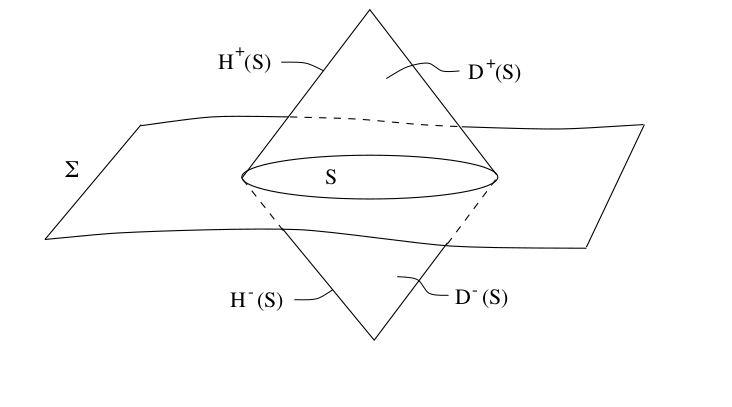
\includegraphics[width=0.7\linewidth]{gfx/CauchyHorizonsGR}
 	\caption{}
 	\label{fig:cauchyhorizonsgr}
 \end{figure}
 
 
 (not necessarily geodesics). We define the \emph{future domain of dependence} of $S$, denoted
 $D_+ (S)$, as the set of all points $p$ such that every past-moving, timelike or null, inextendible
 curve through $p$ must intersect $S$. (“Inextendible” just means that the curve goes on forever,
 not ending at some finite point.) We interpret this definition in such a way that $S$ itself is a
 subset of $D_+ (S)$. (Of course a rigorous formulation does not require additional interpretation
 over and above the definitions, but we are not being as rigorous as we could be right now.)
 Similarly, we define the \emph{past domain of dependence} $D_− (S)$ in the same way, but with “past-
 moving” replaced by “future-moving.” Generally speaking, some points in $M$ will be in one
 of the domains of dependence, and some will be outside; we define the boundary of $D_+ (S)$
 to be the \emph{future Cauchy horizon} $H_+ (S)$, and likewise the boundary of $D_− (S)$ to be the
 \emph{past Cauchy horizon} $H_− (S)$. You can convince yourself that they are both null surfaces.
 \\
 The usefulness of these definitions should be apparent; if nothing moves faster than light,
 than signals cannot propagate outside the light cone of any point $p$. Therefore, if every
 curve which remains inside this light cone must intersect $S$, then information specified on $S$
 should be sufficient to predict what the situation is at $p$. (That is, initial data for matter
 fields given on $S$ can be used to solve for the value of the fields at $p$.) The set of all points
 for which we can predict what happens by knowing what happens on $S$ is simply the union
 $D_+ (S) \cup D_− (S)$.\\
 \\
 We can easily extend these ideas from the subset $S$ to the entire hypersurface $Σ$. The
 important point is that $D_+ (Σ) \cup D_− (Σ)$ might fail to be all of $M$, even if $Σ$ itself seems like
 a perfectly respectable hypersurface that extends throughout space. There are a number
 of ways in which this can happen.
 Glossed over Misner space example and Minkowski space example.
 \\
 A final example is provided by the existence of singularities, points which are not in the
 manifold even though they can be reached by travelling along a geodesic for a finite distance.
 Typically these occur when the curvature becomes infinite at some point; if this happens,
 the point can no longer be said to be part of the spacetime. Such an occurrence can lead to
 the emergence of a Cauchy horizon — a point $p$ which is in the future of a singularity cannot
 be in the domain of dependence of a hypersurface to the past of the singularity, because
 there will be curves from $p$ which simply end at the singularity.
 \begin{figure}[h!]
 	\centering
 	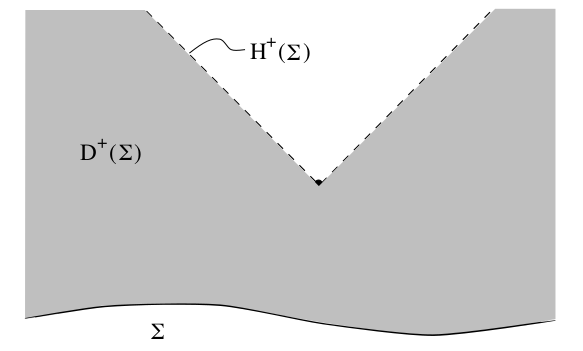
\includegraphics[width=0.7\linewidth]{gfx/SingularitiesGR}
 	\caption{}
 	\label{fig:singularitiesgr}
 \end{figure}
 Singularities are practically unavoidable. The simple fact that the gravitational force is always attractive
 tends to pull matter together, increasing the curvature, and generally leading to some sort of
 singularity. This is something which we apparently must learn to live with, although there
 is some hope that a well-defined theory of quantum gravity will eliminate the singularities
 of classical GR.
 
 
 
 
 
 
 
 
 
 
 \subsection{Hawking-Penrose Singularity Theorems: TO DO}
 \label{subsec:HawkingPenroseSingularity}
 A singularity in solutions of the Einstein field equations is one of two things:\\
 \begin{enumerate}
 	\item
 	a situation where matter is forced to be compressed to a point (a space-like singularity)
 	\item a situation where certain light rays come from a region with infinite curvature (a time-like singularity)
 	Space-like singularities are a feature of non-rotating uncharged black-holes, while time-like singularities are those that occur in charged or rotating black hole exact solutions. Both of them have the property of \emph{geodesic incompleteness}, in which either some light-path or some particle-path cannot be extended beyond a certain proper-time or affine-parameter (affine-parameter being the null analog of proper-time).
 \end{enumerate}
 The Penrose theorem guarantees that some sort of geodesic incompleteness occurs inside any black hole whenever matter satisfies reasonable energy conditions (It does not hold for matter described by a super-field, i.e., the Dirac field). The energy condition required for the black-hole singularity theorem is weak: it says that light rays are always focused together by gravity, never drawn apart, and this holds whenever the energy of matter is non-negative.\\
 \\
 
 Hawking's singularity theorem is for the whole universe, and works backwards in time: it guarantees that the (classical) Big Bang has infinite density.[1] This theorem is more restricted and only holds when matter obeys a stronger energy condition, called the \emph{dominant energy condition}, in which the energy is larger than the pressure. All ordinary matter, with the exception of a vacuum expectation value of a scalar field, obeys this condition. During inflation, the universe violates the dominant energy condition, and it was initially argued (e.g. by Starobinsky[2]) that inflationary cosmologies could avoid the initial big-bang singularity. However, it has since been shown that inflationary cosmologies are still past-incomplete[3], and thus require physics other than inflation to describe the past boundary of the inflating region of spacetime.\\
 \\
 
 It is still an open question whether (classical) general relativity predicts time-like singularities in the interior of realistic charged or rotating black holes, or whether these are artefacts of high-symmetry solutions and turn into spacelike singularities when perturbations are added.\\
 \\
 
 In general relativity, a singularity is a place that objects or light rays can reach in a finite time where the curvature becomes infinite, or space-time stops being a manifold. Singularities can be found in all the black-hole spacetimes, the Schwarzschild metric, the Reissner–Nordström metric, the Kerr metric and the Kerr–Newman metric and in all cosmological solutions that do not have a scalar field energy or a cosmological constant.\\
 \\
 
 One cannot predict what might come "out" of a big-bang singularity in our past, or what happens to an observer that falls "in" to a black-hole singularity in the future, so they require a modification of physical law. Before Penrose, it was conceivable that singularities only form in contrived situations. For example, in the collapse of a star to form a black hole, if the star is spinning and thus possesses some angular momentum, maybe the centrifugal force partly counteracts gravity and keeps a singularity from forming. The singularity theorems prove that this cannot happen, and that a singularity will always form once an event horizon forms.
 \\
 \\
 In the collapsing star example, since all matter and energy is a source of gravitational attraction in general relativity, the additional angular momentum only pulls the star together more strongly as it contracts: the part outside the event horizon eventually settles down to a Kerr black hole (see No-hair theorem). The part inside the event horizon necessarily has a singularity somewhere. The proof is somewhat constructive – it shows that the singularity can be found by following light-rays from a surface just inside the horizon. But the proof does not say what type of singularity occurs, spacelike, timelike, orbifold, jump discontinuity in the metric. It only guarantees that if one follows the time-like geodesics into the future, it is impossible for the boundary of the region they form to be generated by the null geodesics from the surface. This means that the boundary must either come from nowhere or the whole future ends at some finite extension.\\
 \\
 
 An interesting "philosophical" feature of general relativity is revealed by the singularity theorems. Because general relativity predicts the inevitable occurrence of singularities, the theory is not complete without a specification for what happens to matter that hits the singularity. 
 
 
 
 
 
 
 
 
 
 
 
 
 
 
 
 
 
 
 
 
 
 
 
 
 
 
 
 
 
 
 
 
 
 
 
 
 
 
 
 
 
 
 
 
 
 
 



\chapter{Applications of General Relativity}
\label{ch:GRapplications}


\section{Weak Gravitational Fields}
When we first derived Einstein’s equations, we checked that we were on the right track by
considering the Newtonian limit. This amounted to the requirements that the gravitational
field be weak, that it be static (no time derivatives), and that test particles be moving slowly.
In this section we will consider a less restrictive situation, in which the field is still weak but
it can vary with time, and there are no restrictions on the motion of test particles. This
will allow us to discuss phenomena which are absent or ambiguous in the Newtonian theory,
such as gravitational radiation (where the field varies with time) and the deflection of light
(which involves fast-moving particles).












\section{Gauge transformations in general relativity}
\subsection{Firstly, remark on the difference to diffeomorphism invariance, aka general covariance}
Gauge invariance is a property where a given field is generated by more than one potential. While a field is unique, the potential that generates it need not be.
The difference between gauge invariance and general covariance, aka diffeomorphism invariance is that the potential is a function of the coordinates, and it generates a field. The field is unique, but there may be many potentials that can generate it.\\
General covariance now is the ability to choose coordinates for general relativity as we like. This must be done carefully, utilizing symmetries and invariance arguments to make sure such transformations are allowable in specific situations.
\marginpar{ The laws of physics as we know them (standard model plus gravity) have gauge transformations that split into two separate, independent parts; transformations of the fields vs transformations of the coordinate system.  Supersymmetry uses a gauge transformation that combines coordinate and field transformations together.}
\\
\\
Equivalently formulated:\\
\begin{mybox}{Difference between gauge invariance and diffeomorphism invariance}
	\emph{A diffeomorphism is the same thing as a smooth coordinate transformation}, which is the same thing as saying that you can switch between two coordinate maps and \emph{leave the physical laws invariant}.\\ 
	There is also gauge invariance, which states that the laws (of physics, usually) remain invariant under a \emph{redefinition} of the fields (a transformation of the fields) that appear in the laws, e.g. in GR the field is $g\munu$ while in QED the field is redefined via a local $U(1)$ transformation as $\psi \rightarrow e^{i \alpha} \psi = \psi^\prime$.  However, coordinate transformations are equivalent to transformations of the fields (there's no difference between moving your coordinate frame to the left, by a metre, and moving all the fields to the right, by a metre, for example), so \emph{coordinate transformations are also a form of gauge transformations}.\\
	\\
	Note that forces arise from redefinitions - called \emph{local gauge transformations} - that vary in time and space.  The forces of the standard model of particle physics arise from local transformations of the fields.  Gravity arises from local coordinate invariance.
\end{mybox}
A gauge-invariant system is not just, as many people misconceive, a system with a local symmetry. Gauge symmetry isn’t really a symmetry in any case, it’s due to a redundancy in the system. Now we see that general relativity is an instance of a gauge-invariant theory too because since the theory does not care about my choice of coordinates, then it has such redundancies which are exactly the values of the coordinates in a chosen coordinate system. In “ordinary” 4-dimensional general relativity, I only need two local degrees of freedom to describe the physics of the theory, whereas the basic object that characterises gravity in the theory, namely the spacetime metric, naively has $10$ degrees of freedom; clearly there’s $8$ too many! Transformations among these redundant degrees of freedom are precisely implemented by diffeomorphisms in GR, consequently diffeomorphisms are the gauge “symmetry” of GR.


\subsection{On General Covariance and gauge symmetry by Weinberg}
As described in \ref{sec:generalcovariance}, General covariance is not an ordinary symmetry principle like Lorentz invariance, but is rather a dynamical principle that governs the effect of gravitational fields. As such, it bears a strong resemblance to another "dynamic symmetry", local gauge invariance, which governs the effects of electromagnetic fields. Local gauge invariance says that the differential equations satisfied by a set of charged fields $\psi(x)$ and the electromagnetic potential $A_\alpha(x)$ retain the same form when these fields are subjected to the transformations
\begin{equation}
\label{eq:EMgaugetrafo}
	\psi(x) \rightarrow \psi(x) e^{i e \varphi(x)}, \quad A_\alpha(x) \rightarrow A_{\alpha} (x) + \frac{\partial }{\partial x^\alpha} \varphi(x),
\end{equation}
thus the fields are transformed and not the coordinates as described above, where $e$ is the charge of the particle represented by $\psi$ and $\varphi(x)$ is an arbitrary function of the space-time coordinates $x^\alpha$. How are we to construct gauge-invariant equations ? Note that derivatives of a charged field $\psi$ do not behave under gauge transformations like $\psi$, but rather
\begin{equation}
	\frac{\partial}{\partial x^\alpha} \psi(x) \rightarrow \frac{\partial}{\partial x^\alpha }\left[\psi (x)e^{i e \varphi(x)} \right]=e^{ie\varphi(x)} \left[\frac{\partial \psi(x)}{\partial x^\alpha} + i e \psi(x) \frac{\partial \varphi(x)}{\partial x^\alpha}\right]
\end{equation}
just as derivatives of tensors do not behave like tensors under general coordinate transformations. It follows that an equation such as
\begin{equation}
	\left(\partial^2 - m^2\right) \psi(x) =0,\qquad \partial^2\equiv \eta^{\alpha  \beta} \frac{\partial}{\partial x^\alpha} \frac{\partial}{\partial x^\beta}
\end{equation}
is \emph{not} gauge-invariant, just as it is not generally covariant. Also note that the electromagnetic potential $A_\mu(x)$ obeys the inhomogeneous transformation law, just as the affine connection coefficients $\Gamma^\alpha\munu$ obeys the inhomogeneous transformation law \ref{eq:christoffelTrafo} for general coordinate transformations. In tensor analysis we put together derivatives of tensors and the affine connection coefficients $\Gamma$ to form "covariant derivatives" that transform like tensors. In electrodynamics we put together derivatives of fields and the vector potential to form "gauge-covariant derivatives"
\begin{equation}
	D_\alpha \psi(x) \equiv \left[\frac{\partial}{\partial x^\alpha} - i e A_\alpha(x)\right]\psi(x)
\end{equation}
that transform like the fields themselves,
\begin{equation}
	D_\alpha \psi(x) \quad \rightarrow \quad [D_\alpha(x) \psi(x)]e^{i e \varphi (x)}.
\end{equation}
An equation that is invariant under gauge transformations with $\varphi$ constant (such invariance is simply tantamount to charge conservation) will be invariant under the general gauge transformation \ref{eq:EMgaugetrafo} provided that it is constructed only out of fields $\psi(x)$ and their gauge.covariant derivatives $D_\alpha \psi(x)$, just as an equation that is invariant under Lorentz transformations will be invariant under general coordinate transformations provided that it is constructed out of tensor and their covariant derivatives. For instance, we can write a gauge-invariant equation that might represent the effect of electromagnetism on a charged scalar field $\psi(x)$ as
\begin{equation}
	\left[\eta^{\alpha \beta} D_\alpha D_\beta + m^2\right] \psi(x) = 0.
\end{equation}
One important property of such theories is that they admit the construction of a conserved gauge-invariant current; in this example we can define
\begin{equation}
	J_\alpha(x) \equiv -i e\left[\psi^\dagger (x) D_\alpha\psi(x) - \psi(x) [D_\alpha\psi(x)]^\dagger\right]
\end{equation}
(A dagger denotes complex conjugation, or in quantum theories the Hermitian adjoint.) That this is gauge invariant is obvious; to see that it is conserved, we write
\begin{equation}
\frac{\partial}{\partial x^\alpha} J^\alpha(x) = \dots = \psi^\dagger(x) D^\alpha D_\alpha\psi(x) - \psi(x) [D^\alpha D_\alpha\psi(x)]^\dagger
\end{equation}
and using the gauge-invariant Klein-Gordon equation above this gives
\begin{equation}
	\frac{\partial}{\partial x^\alpha} J^\alpha(x) =0.
\end{equation}
We can use this current in the RHS of Maxwell's equations and these equations will then be gauge-invariant also. We see later on that the field equations for gravitation are constructed in an analogous manner.\\
The analogy between the gauge invariance of electrodynamics and the general covariance of GR can be extended to a similar dynamic symmetry, called chirality.

















\subsection{Finding the gauge class}
With the linearised field equations at hand, we are almost prepared to set about solving
them. First, however, we should deal with the thorny issue of gauge invariance. This issue
arises because the demand that $g_{μν} = η_{μν} + h_{μν}$ does not completely specify the coordinate
system on spacetime; there may be other coordinate systems in which the metric can still
be written as the Minkowski metric plus a small perturbation, but the perturbation will be
different. Thus, the decomposition of the metric into a flat background plus a perturbation
is not unique.\\\
Two possible equivalent viewpoints:
\begin{enumerate}
	\item We can think about this from a highbrow point of view. The notion that the linearized
theory can be thought of as one governing the behaviour of tensor fields on a flat background
can be formalized in terms of a “background spacetime” $M_b$ , a “physical spacetime” $M_p$ ,
and a diffeomorphism $\phi : M_b → M_p$ . As manifolds $M_b$ and $M_p$ are “the same” (since
they are diffeomorphic), but we imagine that they possess some different tensor fields; on
$M_b$ we have defined the flat Minkowski metric $η_{μν}$ , while on $M_p$ we have some metric $g_{αβ}$
which obeys Einstein’s equations. (We imagine that $M_b$ is equipped with coordinates $x^μ$ and
$M_p$ is equipped with coordinates $y^α$ , although these will not play a prominent role.) The
diffeomorphism $\phi$ allows us to move tensors back and forth between the background and
physical spacetimes. Since we would like to construct our linearized theory as one taking
place on the flat background spacetime, we are interested in the pullback $(\phi^∗ g)_{μν}$ of the
physical metric. We can define the perturbation as the difference between the pulled-back
physical metric and the flat one:
\begin{equation}
	h_{\mu \nu} = (\phi^* g)_{\mu \nu} -\eta_{\mu \nu}.
\end{equation}
From this definition, there is no reason for the components of $h_{μν}$ to be small; however, if the
gravitational fields on $M_p$ are weak, then for some diffeomorphisms $\phi$ we will have $|h_{μν} | \ll 1$.
We therefore limit our attention only to those diffeomorphisms for which this is true. Then
the fact that $g_{αβ}$ obeys Einstein’s equations on the physical spacetime means that $h_{μν}$ will
obey the linearized equations on the background spacetime (since $\phi$, as a diffeomorphism,
can be used to pull back Einstein’s equations themselves).

\begin{figure}[h!]
	\centering
	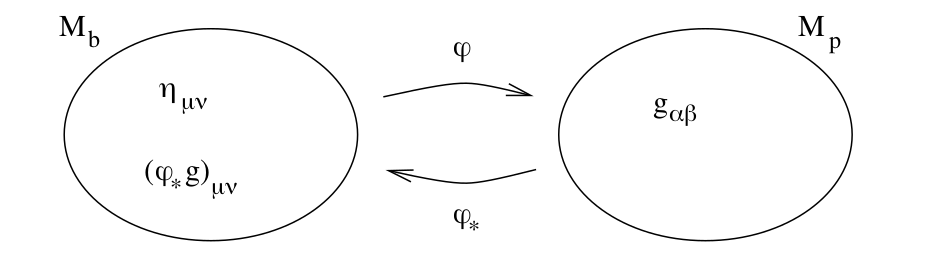
\includegraphics[width=0.7\linewidth]{gfx/GaugeInvarianceGR}
	\caption{}
	\label{fig:gaugeinvariancegr}
\end{figure}





\begin{statements}
	\textbf{In this language, the issue of gauge invariance is simply the fact that there are a large
	number of permissible diffeomorphisms between $M_b$ and $M_p$ (where “permissible” means that the perturbation is small).}
\end{statements}
Consider a vector field $\xi^μ (x)$ on the background spacetime.
This vector field generates a one-parameter family of diffeomorphisms $ψ_\epsilon : M_b → M_b$ . For
$\epsilon$ sufficiently small, if $\phi$ is a diffeomorphism for which the perturbation defined by $	h_{\mu \nu} = (\phi^* g)_{\mu \nu} -\eta_{\mu \nu}.$ is
small than so will $(\phi \circ ψ_\epsilon )$ be, although the perturbation will have a different value.
\begin{figure}[h!]
	\centering
	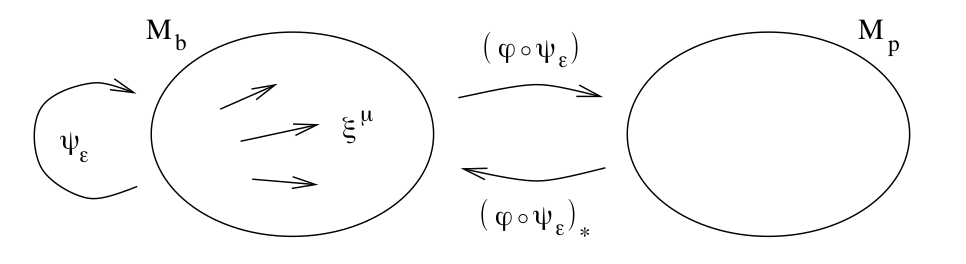
\includegraphics[width=0.7\linewidth]{gfx/GaugeInvarianceGr2}
	\caption{}
	\label{fig:gaugeinvariancegr2}
\end{figure}

Specifically, we can define a family of perturbations parameterized by $\epsilon$:
\begin{align*}
	h^{(\epsilon )}_{\mu \nu} &= [(\phi \circ ψ_\epsilon )_* g]_{ μν} − η_{μν}\\
	&= [ψ_{\epsilon_*} (φ_* g)]_{ μν} − η_{ μν}.
\end{align*}
The second equality is based on the fact that the pullback under a composition is given by
the composition of the pullbacks in the opposite order, which follows from the fact that the
pullback itself moves things in the opposite direction from the original map. Plugging in the
perturbation, we find
\begin{align}
	h^{(\epsilon)}_{\mu \nu} &= ψ_{\epsilon_*} (h + η)_{μν} − η_{μν} \\
	&= \psi_{\epsilon_*}(h_{\mu\nu}) + \psi_{\epsilon_*} (\eta_{\mu \nu}) - \eta_{\mu \nu} 
\end{align}
(since the pullback of the sum of two tensors is the sum of the pullbacks). Now we use our
assumption that $\epsilon$ is small; in this case $\psi_{\epsilon_*}(h_{μν} )$ will be equal to $h_{μν}$ to lowest order, while
the other two terms give us a Lie derivative:
\begin{align}
	\label{eq:GaugefreedomGR}
	h^{(\epsilon)}_{\mu \nu} &= \psi_{\epsilon_*}(h_{\mu \nu}) + \epsilon \left[ \frac{\psi_{\epsilon_*}(\eta_{\mu \nu}) - \eta_{\mu \nu}}{\epsilon}\right]\\
	&= h\munu +\epsilon \mL_\xi \eta_{\mu \nu} \\
	&= h\munu + 2 \epsilon \partial_{(\mu}\xi_{\nu)}.
\end{align}
The last equality follows from our previous computation of the Lie derivative of the metric \ref{eq:liederivMetric}, plus the fact that covariant derivatives are simply partial derivatives to lowest order.\\
\textbf{The infinitesimal diffeomorphisms $\psi_{\epsilon}$ provide a different representation of the same physical situation, while maintaining our requirement that the perturbation be small. Therefore,
the result \ref{eq:GaugefreedomGR} tells us what kind of metric perturbations denote physically equivalent
spacetimes — those related to each other by $2\epsilon ∂_{ (μ} ξ_{ ν)}$ , for some vector $ξ^μ$ }. The invariance of our theory under such transformations is analogous to traditional gauge invariance of electromagnetism under $A_μ → A_μ + ∂_μ λ$. (The analogy is different from the previous analogy
we drew with electromagnetism, relating local Lorentz transformations in the orthonormal-
frame formalism to changes of basis in an internal vector bundle.) In electromagnetism the
invariance comes about because the field strength $F_{μν} = ∂_μ A_ν − ∂_ν A_μ$ is left unchanged
by gauge transformations; similarly, \textbf{we find that the transformation \ref{eq:GaugefreedomGR} changes the linearised Riemann tensor by $\delta R_{\mu \nu \rho \sigma}=0$, i.e. the physical situations are the same},  as was computed in exercises. Our abstract derivation of the appropriate gauge transformation for the metric perturbation is verified by the fact that it leaves the curvature (and hence the physical spacetime)
unchanged.

\item Gauge invariance can also be understood from the slightly more lowbrow but considerably
more direct route of infinitesimal coordinate transformations. Our diffeomorphism $ψ_\epsilon$ can
be thought of as changing coordinates from $x^μ$ to $x^μ − \epsilon ξ^μ$ . (The minus sign, which is
unconventional, comes from the fact that the “new” metric is pulled back from a small
distance forward along the integral curves, which is equivalent to replacing the coordinates
by those a small distance backward along the curves.) Following through the usual rules for
transforming tensors under coordinate transformations, you can derive precisely \ref{eq:GaugefreedomGR} —
although you have to cheat somewhat by equating components of tensors in two different
coordinate systems, c.f. Weinberg.
\end{enumerate}
When faced with a system that is invariant under some kind of gauge transformations,
our first instinct is to fix a gauge. We have already discussed the harmonic coordinate
system, and will return to it now in the context of the weak field limit.
\\
\\
INCORPORATE INTO THE ABOVE:\\
What is gauge invariance ?\\
The equations of physics are invariant when we make  coordinate displacements any constant amount $a^\mu$ :
\begin{equation}
x^{\mu^\prime} = x^\mu +a^\mu.
\end{equation}
To make it formally more like the phase (in qm. $\psi^\prime = e^{ia} \psi$) and isospin (Yang-Mills vector meson theory: $\psi^\prime = e^{i \vec{\tau}\cdot \vec{a}} \psi$, the proposal of Yang and Mills is that a field should be aded to the Lagrangian, in such a way that a \emph{space-dependent} phase change $\vec{a}\rightarrow \vec{X}$ makes no difference in the equations) transformations, one might use the momentum representation so that the translation operator is
\begin{equation}
\exp(i p_\mu a^\mu).
\end{equation}
On the other hand, it is possible to investigate how we might make the equations of physics invariant when we allow space dependent \emph{variable} displacements $a^\mu \rightarrow \zeta^\mu$. The search will be for a more complete Lagrangian, the new terms that are needed are precisely those of a gravity field. Thus, gravity is that field which corresponds to a gauge invariance with respect to displacement transformations. MORE LATER






\subsection{Linearised theory of gravity}
\marginpar{Excellently satisfied in the solar system or galaxy cluster with high $\Phi \Rightarrow$ Pull indices up and down with $\eta_{\mu \nu}$ and not $g_{\mu\nu}$ to remain leading order $\mathcal{O}(h^2)$.}
Study solutions for the field equations in the case of an almost Minkowskian metric, i.e with small perturbation
\begin{equation}
g_{\mu \nu} = \eta_{\mu \nu} + h_{\mu \nu}, 
\end{equation}
with $|h_{\mu \nu}|\ll 1$, this is a coordinate dependent condition, can be violated in other system.
Note that the perturbations
can be split up into \emph{scalar} perturbations $( h_{ 00} , h_{ii} )$, \emph{vector} perturbations ( $h_{0i}$ ) and \emph{tensor} perturbations $h_{i j}$ . At
first order they correspond to gravitational potentials, gravitomagnetic effects and waves respectively.\\
 \\
We can think of
the linearised version of general relativity (where effects of higher than first order in $h_{μν}$
are neglected) as describing a theory of a symmetric tensor field $h_{μν}$ propagating on a flat
background spacetime. This theory is Lorentz invariant in the sense of special relativity;
under a Lorentz transformation $x^{μ^\prime} = Λ^{\mu^\prime}_μ x^μ$ , the flat metric $η_{μν}$ is invariant, while the
perturbation transforms as a symmetric tensor does under Lorentz trafo
(Note that we could have considered small perturbations about some other background
spacetime besides Minkowski space. In that case the metric would have been written $g_{μν} =g^{(0)}_{μν}+ h_{μν}$ , and we would have derived a theory of a symmetric tensor propagating on the
curved space with metric $g^{(0)}_{ μν}$. Such an approach is necessary, for example, in cosmology.)
\\
\\
The weak metric perturbation $h_{\mu \nu}$ admits the gauge transformation
\begin{equation}
	h_{\mu \nu} \rightarrow h_{\mu \nu} + \partial_{\mu} \xi_{\nu} + \partial_{\nu} \xi_{\mu},
\end{equation}
where $\xi=vt$. This is the \emph{gauge class}. One can change $h_{\mu \nu}$ in this way without violating physical laws, this is the \emph{gauge freedom} as described above for the lecture definition of diffeomorphism invariance. Note
that the linearised (in $h$) Ricci tensor is
\begin{equation}
	R\munu =\half η^{αβ}\left[ ∂_μ ∂_β h_{αν} + ∂_α ∂_ν h_{μβ} − ∂_α ∂_β h_{μν} − ∂_μ ∂_ν h_{αβ} \right] 
\end{equation}
is invariant under this gauge transformation, which exemplifies that the gauge transformation relates two situations which are physically \emph{equivalent}.
\begin{mybox}{Gauge theories}
	A gauge theory represents each physically distinct configuration of the system as an equivalence class of detailed local field configurations. Any two detailed configuration in the same equivalence class are related by a gauge transformation, as e.g. above.
\end{mybox}
\begin{mybox}{Hilbert gauge}
The harmonic gauge $\nabla^\nu \nabla_\nu x^\mu=g^{\rho \lambda} \Gamma^\mu_{\rho \lambda}=0$ in the weak field limit is equivalent to
\begin{equation}
\label{eq:Hilbertgauge}
	\half \eta^{\mu \nu} \eta^{\lambda \rho} \left[\partial_{(\mu} h_{\nu \lambda} + \partial_{\nu} h_{\lambda \mu} - \partial_{\lambda} h\munu\right]=\underbrace{∂_μ h^\mu_λ −\half  ∂_λ h}_{\partial\mu \gamma^\mu_{\,\, \lambda}} = 0 .
\end{equation}
This condition is also known as \emph{Lorentz gauge (or Einstein gauge or Hilbert gauge or de Don-
der gauge or Fock gauge)}. As before, we still have some gauge freedom remaining, since we
can change our coordinates by (infinitesimal) harmonic functions.
\end{mybox}
Substituting 
\begin{equation}
	\gamma_{\mu \nu} = h_{\mu \nu} - \frac{1}{2} \eta_{\mu \nu} \underbrace{h^a_a}_{:= h}
\end{equation}
and enforcing the \emph{Hilbert gauge condition}
\begin{equation}
	\partial_{\nu} \gamma^{\mu \nu} = 0,
\end{equation}
in order to have gauge invariance made physical $\Leftrightarrow$ coping with redundant degrees of freedom due to the gauge invariance, to find the linearised field equations as
\begin{equation}
\label{eq:eomlinearisedperturbationsGR}
	\square \gamma^{\mu \nu} = -\frac{16 \pi \mathcal{G}}{c^4} T^{\mu \nu}.
\end{equation}
The vacuum equations $R_{μν} = 0$ take on the elegant form
\begin{equation}
\label{eq:eomvacuumlinearisedpeturbationGR}
	\square \gamma_{\mu \nu} =0
\end{equation}
which is simply the conventional relativistic wave equation. Together, \ref{eq:eomvacuumlinearisedpeturbationGR} and \ref{eq:Hilbertgauge}
determine the evolution of a disturbance in the gravitational field in vacuum in the harmonic
gauge.\\
We can use the QED solution (its retarded Green's function) here since both theories are mediated by massless bosons (otherwise Yukawa cut-off $\frac{1}{|x-x'|} \mapsto \frac{1}{|x-x'|} e^{- |x-x'|\lambda}$). \\
Formally being identical to the Maxwell equations, these equations can therefore be solved using the retarded Green's function of Maxwell electrodynamics. Thus, similar to electrodynamics, the metric perturbation consists of the field generated by the source plus wave-like vacuum solution propagating \emph{at} the speed of light, i.e. \emph{gravitational waves} with $v=c$.

\subsection{Nearly Newtonian gravity}
\todo{Go through chapter 10 gravitational radiation by Weinberg and incorporate into this sparse treatment of the topic.}
Now one can insert all kinds of specific sources into $T_{\mu \nu}$ to determine the metric, since $T_{\mu \nu}$ determines $\gamma_{\mu \nu}$.\\
In the non-relativistic case $T_{00} \gg |T_{0j}| \; \& \; T_{00} \gg |T_{ij}|$, we recover the \emph{Newtonian approximation} of the metric.
From \ref{eq:eomlinearisedperturbationsGR} and our previous exploration of the Newtonian limit, it is straightforward to
derive the weak-field metric for a stationary spherical source such as a planet or star. Recall
that previously we found that Einstein’s equations predicted that $h_{00}$ obeyed the Poisson
equation in the weak-field limit, which implied
$h_{00} = −2Φ$, where $Φ$ is the conventional Newtonian potential, $Φ = −GM/r$. Let us now assume that
the energy-momentum tensor of our source is dominated by its rest energy density $ρ = T_{00}$ .
(Such an assumption is not generally necessary in the weak-field limit, but will certainly
hold for a planet or star, which is what we would like to consider for the moment.) Then
the other components of $T\munu$ will be much smaller than $T_{00}$ , and from \ref{eq:eomlinearisedperturbationsGR} the same must
hold for $\gamma_{\mu \nu}$ . If $\gamma_{00}$ is much larger than $\gamma_{ij}$ , we will have
\begin{equation}
	h = -\gamma = -\eta^{\mu \nu} \gamma_{\mu \nu} = \gamma_{00},
\end{equation}
and then we immediately find
\begin{equation}
\gamma_{00} = 2 h_{00} = - 4\Phi.
\end{equation}
The other components of $\gamma_{μν}$ are negligible, from which we can derive
\begin{equation}
	h_{i0} = \gamma_{i0} - \half \eta_{0i}\gamma =0
\end{equation}
and 
\begin{equation}
	h_{ ij} = \gamma_{ij} − \half \eta_{ ij} \gamma = −2Φ δ_{ij}.
\end{equation}
The metric for a star or planet in the weak-field limit is therefore
\begin{equation}
	\md s^2 = -(1+2 \Phi) \md t^2 + (1 -2 \Phi) \md \vec{x}^2.
\end{equation}




\begin{mybox}{Newtonian limit}
	In the Newtonian limit (non-relativistic limit +weak gravitational field+instantaneous propagation of perturbations), the weakly perturbed metric of a mass $M$ has the line element
	\begin{align}
		\md s^2 &= - \left(1+ \frac{2 \Phi}{c^2}\right) c^2 \md t^2 + \left(1-\frac{2 \Phi}{c^2}\right) \md \vec{x}^2,\\
		\Leftrightarrow \md s^2 &=-\left(1 - \frac{2 \mathcal{G}M}{r c^2}\right) c^2 \md t^2 + \left(1+\frac{2 \mathcal{G}M}{r c^2}\right) \md \vec{x}^2\\
		\Rightarrow (g_{\mu \nu}) &= (\eta_{\mu \nu}) - \frac{2 \Phi}{c^2} \mathcal{I}_{4\times 4}.
	\end{align}
\end{mybox}

Thus, the full theory has space-time curvature \emph{and} not only spatial curvature.\\
Note: \\
Although we have now imposed the harmonic gauge condition, there is still some coordinate freedom left. Remember that any coordinate transformation of the form
$x^μ → x^μ + ζ^μ$ will leave the harmonic coordinate condition $\nabla^\alpha \nabla_\alpha x^μ = 0$ satisfied as long as we have $\nabla^\alpha \nabla_\alpha ζ^μ = 0$.
Conclusions:
\begin{enumerate}
	\item Light follows null geodesics $\md s^2=0 \Rightarrow$ velocity of light in gravitational field is less than $c$:
	\begin{equation}
	\frac{\md \vec{x}^2}{\md t^2} = c^2 \frac{\left(1+\frac{2 \Phi}{c^2}\right)}{\left(1-\frac{2 \Phi}{c^2}\right)} =: (c')^2 \; \Rightarrow \; c' = \frac{c}{n}, n \approxeq 1-\frac{2 \Phi}{c^2}.
	\end{equation}
	\begin{mybox}{Gravitational Lensing}
		A weak gravitational field with Newtonian gravitational potential $\Phi$ has the effective index of refraction
		\begin{equation}
		n = 1- \frac{2 \Phi}{c^2} \geq 1, 
		\end{equation}
		$\Rightarrow$ optically denser medium than vacuum\\
		$\Rightarrow$ Light deflection, light rays are bent in a gravitational field.
	\end{mybox}
	\item \emph{Clocks go slower in a gravitational field}:\\
	\marginpar{The gravitational potentials are negative, so that clock should run more slowly as they come nearer to a massive object such as a star.}
	Compared to light propagation in vacuum, there is thus a \emph{time delay}
	\begin{equation}
		\Delta(\md t) = \md t-\frac{\md l}{c} = - \frac{2 \Phi}{c^3} \md l,
	\end{equation}
	with $\md t=\frac{\md l}{c'}= n \frac{\md l}{c}$ the light travel time along an infinitesimal path length $\md l$ in a gravitational field (hence $c'$).\\
	With respect to whom do clocks go slower ?\\
	Suppose two clocks are at rest. The clock that is under the influence of a stronger gravitational
	field (i.e. it is closer to a massive object) ticks slower than the other clock experiencing a weaker
	gravitational field (i.e. it is farther away from the massive object).
\end{enumerate}

Introducing outer source $T_{\mu \nu}$ leads to the \emph{gravitomagnetic field}. Only approximate $T_{ij}=0$ (no stresses) and define $A_{\mu} = \gamma_{0 \mu} /4$ to find
\begin{equation}
	\square A_{\mu} = - \frac{4 \pi}{c^2} \underbrace{j_{\mu}}_{=\frac{\mathcal{G}T_{0 \mu}}{c^2}}.
\end{equation}
This similarity to electrodynamics leads to the introduction of "electric" and "magnetic" components of the gravitational field.
\begin{statements}
	Matter currents create a magnetic gravitational potential $A_{\mu}$ ("gravitomagnetic potential") similar to the em. vector potential $A_{\nu}$.
\end{statements}
$\Rightarrow T_{\mu \nu}$ yields the metric, which in turn yields the e.o.m. via the variational principle !.\\
\marginpar{This treatment is only an analogy! If you have to take matter currents $T_{0j}$ into account in gavitational field, then you get similar behaviour as in ED. Before we only used matter densities.}
$\Rightarrow$ One recovers e.o.m. which exhibit a "magnetic" Lorentz force term and a gravitational term. Its effect on a spinning test particle is the \emph{gravito-magnetic force} $\vec{f} = c^2\vec{\nabla} A_0 + 4 c \vec{v} \times \vec{B}$, with $\vec{B}:= \vec{\nabla} \times \vec{A}$, lets the test particles' angular momentum experience a torque:
\begin{mybox}{Lense-Thirring effect or space time frame drag}
	A spinning body in a gravitomagnetic field will experience spin precession with the angular frequency \begin{equation}
		\vec{\omega} = -2 c \vec{B} = - 2 c\vec{\nabla }\times \vec{A},
	\end{equation}
	which is called the Lense-Thirring effect.\\
	$\Leftrightarrow$ A rotating body drag the gravitational field in its vicinity around.\\
	It predicts that the rotation of a massive object would distort the spacetime metric, making the orbit of a nearby test particle precess. This does not happen in Newtonian mechanics for which the gravitational field of a body depends only on its mass, not on its rotation. The Lense–Thirring effect is very small—about one part in a few trillion. To detect it, it is necessary to examine a very massive object, or build an instrument that is very sensitive.
\end{mybox}

Frame-dragging is an effect on spacetime that is due to non-static stationary distributions of mass–energy. A stationary field is one that is in a steady state, but the masses causing that field may be non-static, rotating for instance. More generally, the subject of effects caused by mass–energy currents is known as gravitomagnetism, in analogy with classical electromagnetism. The Lense-Thirring effect is one spacetime frame dragging effect, the rotational frame-dragging.
\\
The possible frame-dragging effects are:\\
\begin{enumerate}
	\item \emph{Rotational frame-dragging (the Lense–Thirring effect)} appears in the general principle of relativity and similar theories in the vicinity of rotating massive objects. 
	Under the Lense–Thirring effect, the frame of reference in which a clock ticks the fastest is one which is revolving around the object as viewed by a distant observer. This also means that light travelling in the direction of rotation of the object will move past the massive object faster than light moving against the rotation, as seen by a distant observer. It is now the best known frame-dragging effect, partly thanks to the Gravity Probe B experiment. Qualitatively, frame-dragging can be viewed as the gravitational analogue of electromagnetic induction.\\
	\\	
	Also, an inner region is dragged more than an outer region. This produces interesting locally rotating frames. For example, imagine that a north-south–oriented ice skater, in orbit over the equator of a black hole and rotationally at rest with respect to the stars, extends her arms. The arm extended toward the black hole will be "torqued" spinward due to gravitomagnetic induction ("torqued" is in quotes because gravitational effects are not considered "forces" under GR). Likewise the arm extended away from the black hole will be torqued anti-spinward. She will therefore be rotationally sped up, in a counter-rotating sense to the black hole. This is the opposite of what happens in everyday experience. There exists a particular rotation rate that, should she be initially rotating at that rate when she extends her arms, inertial effects and frame-dragging effects will balance and her rate of rotation will not change. Due to the equivalence principle, gravitational effects are locally indistinguishable from inertial effects, so this rotation rate, at which when she extends her arms nothing happens, is her local reference for non-rotation. This frame is rotating with respect to the fixed stars and counter-rotating with respect to the black hole. This effect is analogous to the hyperfine structure in atomic spectra due to nuclear spin. A useful metaphor is a planetary gear system with the black hole being the sun gear, the ice skater being a planetary gear and the outside universe being the ring gear. See Mach's principle.\\
	\\
	Another interesting consequence is that, for an object constrained in an equatorial orbit, but not in freefall, it weighs more if orbiting anti-spinward, and less if orbiting spinward. For example, in a suspended equatorial bowling alley, a bowling ball rolled anti-spinward would weigh more than the same ball rolled in a spinward direction. Note, frame dragging will neither accelerate nor slow down the bowling ball in either direction. It is not a "viscosity".\todo{What does that mean, how is the equivalence and not feeling gravity compatible with this ? EP says that gravity is not distinct able from an acceleration, but the objects weighs more moving against or less if moving with rotation of the BH ? } Similarly, a stationary plumb-bob suspended over the rotating object will not list. It will hang vertically. If it starts to fall, induction will push it in the spinward direction.
	
	\item \emph{Linear frame dragging} is the similarly inevitable result of the general principle of relativity, applied to linear momentum. Although it arguably has equal theoretical legitimacy to the "rotational" effect, the difficulty of obtaining an experimental verification of the effect means that it receives much less discussion and is often omitted from articles on frame-dragging (but see Einstein, 1921).
	
	\item \emph{Static mass increase} is a third effect noted by Einstein in the same paper. The effect is an increase in inertia of a body when other masses are placed nearby. While not strictly a frame dragging effect (the term frame dragging is not used by Einstein), it is demonstrated by Einstein that it derives from the same equation of general relativity. It is also a tiny effect that is difficult to confirm experimentally.
	
	
\end{enumerate}


















\section{Gravitational Waves - The propagation of the metric perturbations}
\todo{This is treated in way more detail in Caroll, c.f. page 148.}
Describing gravitational perturbations as superposition of plane waves
\begin{equation}
	\gamma_{\mu \nu} = \mathrm{Re}\{ \epsilon_{\mu \nu} e^{i \langle k,x\rangle} \},
\end{equation}
\marginpar{For gauge trafo $h_{\mu \nu} \rightarrow h_{\mu \nu} + \partial_{\mu} \xi_{\nu}+\partial_{\nu} \xi_{\mu}$ with
$2 \partial_{\mu}\xi^{\mu}=0, \partial_{\alpha}\partial^{\alpha} \xi^{\mu} =0$ in Hilbert gauge, one has
$\gamma_{\mu \nu}=h_{\mu \nu}$.}
with amplitudes given by the so-called polarisation tensor $\epsilon_{\mu \nu}$, one finds in Hilbert gauge:
\begin{mybox}{Gauge-invariant polarisation states}
	As for electromagnetic waves, there are only two gauge-invariant, linearly independent polarisation states for gravitational waves.\\
	$h=\pm 2 \Rightarrow$ the two polarisation states correspond to left and right-handed circular polarisation.
\end{mybox}
In the limit of far-away source, small velocities and overall rest-mass dominating, one finds 
\marginpar{Em waves are created by time-dependent dipole instead.}
\begin{mybox}{Source of gravitational waves I}
	Wave-like metric perturbations in varuum are created by the second time-derivative of a matter distribution with density $\rho$,
	\begin{align}
		\gamma^{jk} (t,\vec{x}) &= -\frac{2\mathcal{G}}{r c^4} \partial^2_t \int \rho \left(t-\frac{r}{c}, \vec{x}\right) x^{'j} x^{'k} \md^3 x', \\
		\gamma_{jk}(t,\vec{x}) &= -\frac{2 \mathcal{G}}{3 r c^4} \left[\partial^2_t Q_{jk} \left(t-\frac{r}{c}, \vec{x}\right) \right. \nonumber \\
		&\left. + \delta_{jk} \partial^2_t \int r^{'2} \rho \left(t-\frac{r}{c}, \vec{x}'\right) \md^3 x'\right],\\
		Q^{jk} &= \int \left(3 x^j x^k -r^2 \delta^{jk} \right) \rho(\vec{x}) \md^3x,
	\end{align}
where $Q^{jk}$ is the source's quadrupole tensor
\end{mybox}
\begin{mybox}{Source of gravitational waves II}
	In order to generate gravitational waves, a mass distribution needs to have a quadrupole moment with non-vanishing second time derivative.
\end{mybox}
The physical reason is the following. The mass monopole represents the total mass-energy in a system, which is conserved. Thus, it cannot lead to radiation. Similarly, the mass dipole corresponds to the centre of mass of a system and its first derivative represents momentum, which is also a conserved quantity so that the mass dipole cannot emit radiation either. The second derivative of the mass quadrupole, however, does not vanish so that the quadrupole is the lowest-order contribution to gravitational radiation. The gravitational wave produced by an isolated nonrelativistic object is therefore proportional to the second derivative of the quadrupole moment of the energy density at the point where the past light cone of the observer intersects the source. In contrast, the leading
contribution to electromagnetic radiation comes from the changing dipole moment of the
charge density. The difference can be traced back to the universal nature of gravitation. A
changing dipole moment corresponds to motion of the center of density — charge density in
the case of electromagnetism, energy density in the case of gravitation. While there is nothing to stop the center of charge of an object from oscillating, oscillation of the center of mass
of an isolated system violates conservation of momentum. (You can shake a body up and
down, but you and the earth shake ever so slightly in the opposite direction to compensate.)
The quadrupole moment, which measures the shape of the system, is generally smaller than
the dipole moment, and for this reason (as well as the weak coupling of matter to gravity)
gravitational radiation is typically much weaker than electromagnetic radiation.
\\
\\
Einstein's quadrupole formula describes the gravitational-wave luminosity
\begin{equation}
	L_{\mathrm{GW}} = \frac{\mathcal{G}}{5 c^5} \langle \tr(\dddot{Q})^2\rangle.
\end{equation}




























\newpage
\section{The Schwarzschild solution}
\subsection{Stationary and static space-times}
\emph{Stationary Spacetimes} $(M,g)$ are defined to be spacetimes which have a global time-like Killing vector field $K$. This means that observers moving along the integral curves of $K$ do not notice any change. This definition implies that we can introduce coordinates in which the components $g_{\mu \nu}$ of the metric do not depend on time. In these so-called \emph{adapted coordinates} with $g_{\mu \nu}(t)=g_{\mu \nu}$, one transports every point on the manifold along the integral-curve of $K = (\partial_0,0,0)$, i.e. along global time coordinates with ($\mathcal{L}_K g)_{\mu \nu} = 0 = \partial_0 g_{\mu \nu}$.\\
\marginpar{$K$ time-like $\Rightarrow \Sigma$ space-like since $K\perp\Sigma$ at $t=t_0$.}\\
In a stationary space-time with time-like Killing vector field $K$, the \emph{Frobenius condition}
\begin{equation}
	\omega \wedge \md \omega =0
\end{equation}
for the one-form $\omega=K^{\flat}$ is equivalent to the condition
\begin{equation}
	g_{0i}=0, \quad  \Rightarrow K\perp \Sigma \,\mathrm{for\, which} \,t=\mathrm{constant},
\end{equation}
which implies that there is no rotation in spacetime, in adapted coordinates ($\Leftrightarrow \md s^2 = \md s^2_{\Sigma} - \md t^2$ decouples spatial and time contributions).\\
Such space-times are called \emph{static}.\\
$\Rightarrow$ In static spacetimes, the metric can thus be written in the form
\begin{equation}
	g = g_{00}(\vec{x}) c^2 \md t^2 + g_{ij}(\vec{x}) \md x^i \md x^j.
\end{equation}
Saying that $K=\partial_t$ is irrotational means that the vorticity tensor of the corresponding timelike congruence vanishes, thus the Killing vector field is the hypersurface orthogonal $K\perp\Sigma$. One immediate consequence is that the constant time coordinate surfaces $t=t_0$ form a family of (isometric) spatial hyperslices.
\begin{figure}
	\centering
	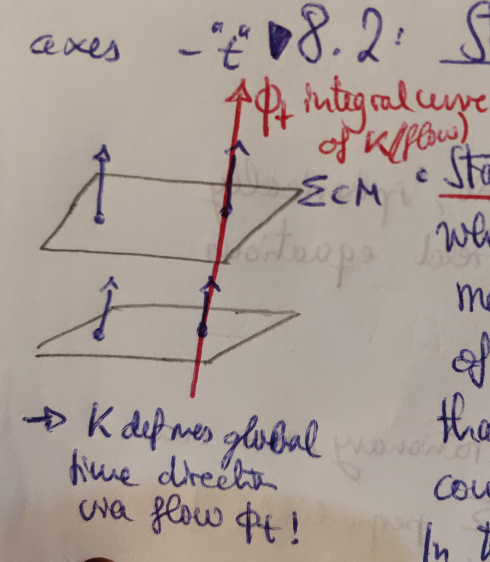
\includegraphics[width=0.7\linewidth]{gfx/staticspacetime}
	\caption{\itshape Foliation of the static spacetime along the fiducial time direction given by global Killing vector field.}
	\label{fig:staticspacetime}
\end{figure}
Roughly speaking, a static metric is one in which nothing is moving,
while a stationary metric allows things to move but only in a symmetric way. For example,
the static spherically symmetric metric (Schwarzschild) will describe non-rotating stars or black holes,
while rotating systems (which keep rotating in the same way at all times) will be described
by stationary metrics.
 \subsection{The Schwarzschild solution}

 The Schwarzschild solution is a static, spherically symmetric solution of Einstein's field equations for vacuum space-time. It describes the gravitational field \emph{outside} a spherical mass, on the assumption that $Q(\mathrm{mass})=\vec{L}(\mathrm{mass})=0=\Lambda$. It works well for slowly rotating astronomical objects (stars, planets). Birkhoff’s theorem states that the
 Schwarzschild solution is the unique spherically symmetric solution to Einstein’s equations
 in vacuum.\\ The Schwarzschild chart is adapted to the spheres $S^2$ nested in Schwarzschild spacetime.\\
 \\
 As the space-time is (globally) stationary, we can introduce spatial hypersurfaces $\Sigma$ perpendicular to the time-like Killing vector field, which in adapted coordinates is $K=\partial_0$. The manifold $(M,g)$ can thus be foliated as $M \cong \mR \times \Sigma$.\\
 \\
 The spatial hypersurfaces $ \Sigma$ are expected to be spherically symmetric, i.e. $SO(3)$ must be an isometry group of the metric $\mathcal{h}$ of the spatial sections 
$h$. The orbits of $SO(3)$ are two-dimensional, space-like surfaces in $\Sigma$. Thus, $SO(3)$ foliates the spacetime $(\Sigma, h)$ into invariant two-spheres.\\
Let the surfaces of these two-spheres be $A$, then we \emph{define} a radial coordinate for the Schwarzschild metric requiring $A=4 \pi r^2$ as in Euclidean geometry. The spherical symmetry further implies that we can introduce spherical polar coordinates $(\vartheta,\varphi)$ on one particular orbit of $SO(3)$ which can then be transported along geodesic lines perpendicular to the orbits.\\
$\Rightarrow$ The spatial sections $\Sigma$ are now foliated according to 
\begin{equation}
	\Sigma = I \times S^2, \; I\subset \mR^+, \quad \mathrm{for} \;r\in I, (\vartheta, \varphi) \in S^2.
\end{equation}
\marginpar{static implies $a(r,t)=a(r)$, such that space-time cannot expand or shrink with time.}
\begin{mybox}{Metric for static, spherically space-times}
	In the Schwarzschild coordinates $(t,r,\vartheta,\varphi)$, the metric of a static, spherically-symmetric space-time has the form
	\begin{equation}
		g = - e^{2 a(r)} c^2 \md t^2 + e^{2 b(r)} \md r^2 + r^2 \md \Omega^2.
	\end{equation}
	The functions $a(r), b(r)$ are constrained by the requirement that the metric should asymptotically turn flat, which means $a(r),b(r) \stackrel{r \rightarrow \infty}{\longrightarrow} 0$, They must be determined by inserting the metric into the vacuum field equations, $G=0$.
\end{mybox}
Introduce tetrad $\{e_i\}$ or alternatively dual-tetrad $\{\theta^i\}$:
\begin{equation}
	\underbrace{\theta^0 = e^a c \md t }_{\Leftrightarrow \theta^0=(e^a,0,0,0)}, \quad \theta^1 = e^b \md r, \quad \theta^2=r \md \vartheta, \quad \theta^3=r \sin\vartheta \md \varphi.
\end{equation}
In terms of this dual-tetrad, the metric attains the simple diagonal, Minkowskian form
\begin{equation}
	g =g_{\mu \nu} \theta^{\mu} \otimes \theta^{\nu}, \qquad g_{\mu \nu} = \mathrm{diag}(-1,1,1,1), \Rightarrow \md g=0.
\end{equation}
For a torsion-free connection, one can then determine the connection form via Cartan $I$ \ref{eq:cartanStructure}. Via Cartan $II$, the curvature forms are found.
\subsection{Solution of the field equations}
With the curvature forms in the given tetrad at hand, one finds the Ricci tensor and thus the Einstein tensor via
\begin{equation}
	R_{\mu \nu} = \bar{R}^{\lambda}_{\mu \lambda \nu} = \Omega^{\lambda}_{\mu}(e_{\lambda}, e_{\nu}).
\end{equation}
\textbf{All off-diagonal components of $G_{\mu \nu}$ vanish identically, which reflects the spherical symmetry of the considered system}.\\
\begin{mybox}{Einstein tensor for a static, spherically-symmetric metric}
	The Einstein tensor of a static, spherically-symmetric metric has the
	components
	\begin{align}
		G_{00} &=\frac{1}{r^2} - E\left(\frac{1}{r^2} - \frac{2 b^\prime}{r}\right), \quad E:= \exp(-2b(r))\\
		G_{11} &=- \frac{1}{r^2}+ E\left(\frac{1}{r^2}+ \frac{2 a^\prime}{r}\right)\\
		G_{22} &= G_{33}.
	\end{align}
All off-diagonal components of $G\munu$ vanish identically.
\end{mybox}
$G_{00}=G_{11}=G_{22}=0$, and thus also $G_{00}+G_{11}=0$ etc, are now differential equations in $a$ and $b$, which can be solved via our boundary condition of asymptotic flatness.
\begin{mybox}{Schwarzschild line element}
	This yields the Schwarzschild solution for the metric,
	\begin{equation}
	\label{eq:Schwarzschildmetric}
		\md s^2 = -\left(1-\frac{2m}{r}\right) c^2 \md t^2 + \frac{\md r^2}{1-\frac{2m}{r}} + r^2 \md \Omega^2.
	\end{equation}
\end{mybox}
Note that $M$ is precisely equal to the total energy of the sun \emph{and its gravitational field} here. The total energy of matter and gravitation here is
\begin{equation}
	P^0 = M,
\end{equation}
where one furthermore finds that the total angular momentum is the expected value zero.

\begin{figure}
	\centering
	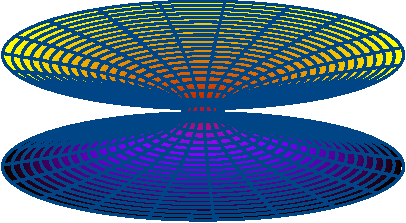
\includegraphics[width=0.7\linewidth]{gfx/schwarzschildMetric}
	\caption{\itshape Schwarzschild spacetime with a physical singularity at $r=0$.}
	\label{fig:schwarzschildmetric}
\end{figure}
In the weak field limit, we have to recover the Newtonian limit $g_{00} \mapsto - (1+\frac{2 \Phi}{c^2})$. We describe a point mass $M$ at the origin with this metric and have $\Phi=-\frac{\mathcal{G}M}{r}$ for $r\gg0$.
\begin{equation}
	\stackrel{\md s^2}{\Rightarrow} \frac{2m}{r} \stackrel{!}{=} \frac{2 \mathcal{G}M}{r c^2} \; \Leftrightarrow\; m:= \frac{\mathcal{G}M}{c^2} = \frac{R_s}{2}.
\end{equation}
The Schwarzschild metric has a coordinate singularity at $r=2m$ or
\begin{equation}
	r=R_s= \frac{2 \mathcal{G}M}{c^2},
\end{equation}
the so-called \emph{Schwarzschild radius}.

\subsubsection{Equivalent forms of the metric}
\begin{enumerate}
	\item We can equivalently express the Schwarzschild metric \ref{eq:Schwarzschildmetric} in the \emph{isotropic form}, by introducing a new radius variable
	\begin{equation}
	\rho \equiv \half \left[r-m+\sqrt{r^2- 2mr}\right] \quad \Leftrightarrow\quad r = \rho (1 + \frac{m}{2 \rho})^2,
	\end{equation}
	which yields the line element
	\begin{equation}
		\md \tau^2 = \left(\frac{1 - \frac{m}{2 \rho}}{1+\frac{m}{2 \rho}}\right)^2 c^2 \md t^2 - \left(1+\frac{m}{2 \rho}\right)^4 \left(\md \rho^2 + \rho^2 \md \theta^2 + \rho^2 \sin^2 \theta \md \varphi^2\right).
	\end{equation}
	\item We can also construct \emph{harmonic coordinates}
	\begin{equation}
		X_1 = R\sin\theta \cos \varphi , \quad X_2 = R\sin\theta\sin\varphi,\quad X_3=R\cos\theta,\quad t
	\end{equation}
	by using for $R$ a solution of a TODO maybe.
\end{enumerate}

\subsection{Birkhoff's theorem}
\label{subsubsec:BirkhoffTheorem}
\begin{mybox}{Birkhoff's theorem}
	In general relativity, Birkhoff's theorem states that any spherically symmetric solution of the vacuum field equations must be static and asymptotically flat. This means that the exterior solution (i.e. the spacetime outside of a spherical, nonrotating, gravitating body) must be given by the Schwarzschild metric.\\
	Thus, a spherically symmetric solution of Einstein's vacuum equations is necessarily static for $r>2m$.\\
	 $\Leftrightarrow$ the Schwarzschild metric is the unique solution to the Einstein equations in vacuum with a spherically symmetric matter distribution.
	 $\Rightarrow$ The matter can oscillate wildly, as long as it remains spherically symmetric, and the gravitational field outside will remain unchanged.
\end{mybox}
\begin{mybox}{Birkhoff's theorem by Weinberg}
	A spherically symmetric gravitational field in empty space must be static, with a metric given by the Schwarzschild solution.
\end{mybox}
The Birkhoff theorem is analogous to the result proved by Newton, that the gravitational field outside a spherically symmetric body behaves as if the whole mass of the body were concentrated at the centre. It is a little surprising that this result should apply in GR as well as in Newton's theory, for in GR a nonstatic body will usually radiate gravitational waves. The Birkhoff theorem tells us that, although a pulsating spherically symmetric body can of course produce nonstatic gravitational fields within its mass, no gravitational radiation can escape into empty space. In this sense, the Birkhoff theorem is analogous to the well-known result of atomic theory, that a photon cannot be emitted in a quantum transition between two states of zero spin.\\
The Birkhoff theorem may be applied, not only to the gravitational field outside a body, but also to the field \emph{inside} an empty spherical cavity at the centre of a spherically symmetric (but not necessarily static) body. In this case the metric is again given by the Schwarzschild solution, but since the point $r=0$ is here in empty space, there can be no singularity.
\begin{mybox}{Corollary of Birkhoff's theorem by Weinberg}
	\emph{The metric inside an empty spherical cavity at the centre of a spherically symmetric system must be equivalent to the flat-space Minkwoski metric} $\eta\munu$.\\
	This corollary is analogous to another famous result of Newtonian theory, that the gravitational field of a spherical shell vanishes inside the shell. Stars do not usually have holes at their centres, so this corollary is not of much use, but it is used later to justify a limited use of Newtonian mechanics in cosmological problems (i.e. it justifies to derive Friedmann's equations from Newtonian physics, but note that the resulting derivation goes beyond Newtonian theory since it assumes Birkhoff's theorem.)
\end{mybox}
\begin{mybox}{Explanation and Implications of Birkhoff's theorem}
The intuitive idea of Birkhoff's theorem is that a spherically symmetric gravitational field should be produced by some massive object at the origin; if there were another concentration of mass-energy somewhere else, this would disturb the spherical symmetry, so we can expect the solution to represent an \emph{isolated} object. That is, the field should vanish at large distances, which is (partly) what we mean by saying the solution is asymptotically flat. Thus, this part of the theorem is just what we would expect from the fact that general relativity reduces to Newtonian gravitation in the Newtonian limit.\\
\\
Implications:\\
The conclusion that the exterior field must also be \emph{stationary} is more surprising, and has an interesting consequence. Suppose we have a spherically symmetric star of fixed mass which is experiencing spherical pulsations. Then Birkhoff's theorem says that the exterior geometry must be Schwarzschild; the only effect of the pulsation is to change the location of the stellar surface. This means that a spherically pulsating star cannot emit gravitational waves.\\
Another interesting consequence of Birkhoff's theorem is that for a spherically symmetric thin shell, the interior solution must be given by the Minkowski metric; in other words, the gravitational field must vanish inside a spherically symmetric shell. This agrees with what happens in Newtonian gravitation.
\end{mybox}

\subsubsection{Remarks on the Schwarzschild metric}
The Schwarzschild metric is true for any spherically symmetric vacuum solution to Einstein’s equations; $M$ functions as a parameter, which we happen to know can be interpreted as the conventional Newtonian mass that we would measure by studying orbits at large distances from the gravitating source. Note that as $M → 0$ we recover Minkowski space, which is to be expected.\\
Note also that the metric becomes progressively Minkowskian as we go to $r → ∞$; this
property is known as \emph{asymptotic flatness}.\\
The fact that the Schwarzschild metric is not just a good solution, but is the unique
spherically symmetric vacuum solution, is known as Birkhoff’s theorem. It is interesting to
note that the result is a static metric. We did not say anything about the source except that
it be spherically symmetric. Specifically, we did not demand that the source itself be static;
it could be a collapsing star, as long as the collapse were symmetric. Therefore a process
such as a supernova explosion, which is basically spherical, would be expected to generate
very little gravitational radiation (in comparison to the amount of energy released through
other channels). This is the same result we would have obtained in electromagnetism, where
the electromagnetic fields around a spherical charge distribution do not depend on the radial
distribution of the charges.











\newpage
\section{Physics in the Schwarzschild Space-Time}

Schwarzschild geodesics describe the motion of particles  of infinitesimal mass in the gravitational field of a central fixed mass $M$, i.e. particles do not themselves contribute to the gravitational field, still very accurate for $m \ll M$. For $M= m_1+m_2$ one can also use Schwarzschild for motion of binary system.
\subsection{A note on the Killing vectors of a Schwarzschild Space-Time}
We know that there are four Killing vectors: three for the spherical
	symmetry, and one for time translations. Each of these will lead to a constant of the motion
	for a free particle. This can simplify calculations.\\
	Rather than immediately writing out explicit expressions for the four conserved quantities
	associated with Killing vectors, let’s think about what they are telling us. Notice that the
	symmetries they represent are also present in flat spacetime, where the conserved quantities
	they lead to are very familiar. Invariance under time translations leads to conservation of
	energy, while invariance under spatial rotations leads to conservation of the three components
	of angular momentum. Essentially the same applies to the Schwarzschild metric. We can
	think of the angular momentum as a three-vector with a magnitude (one component) and
	direction (two components). Conservation of the direction of angular momentum means
	that the particle will move in a plane. We can choose this to be the equatorial plane of
	our coordinate system; if the particle is not in this plane, we can rotate coordinates until
	it is. Thus, the two Killing vectors which lead to conservation of the direction of angular
	momentum imply
	\begin{equation}
		\theta = \frac{\pi}{2}.
	\end{equation}
	The two remaining Killing vectors correspond to energy and the magnitude of angular mo-
	mentum. The energy arises from the timelike Killing vector $K = ∂_t$ , or
	\begin{equation}
		K_\mu = g\munu K^\nu =g_{00} \partial_t= \left(-\left(1-\frac{2\mathcal{G}M}{r}\right),0,0,0\right),
	\end{equation}
	where one gets the components of the Killing vectors via raising or lowering indices with the metric and using that $\partial_t=(1,0,0,0)$ in our adapted coordinate system, i.e. it is the basis vector of the $0$-component in our tangent space where all vectors live.\\
	The Killing vector whose conserved quantity is the magnitude of the angular momentum is
	$L = ∂_φ$ , or
	\begin{equation}
	L_\mu= g\munu L^\mu = g_{\varphi \varphi} \partial_\varphi = r^2 \sin^2\vartheta (0,0,0,1) = \left(0,0,0,r^2 \sin^2 \vartheta\right).
	\end{equation}
We have four Killing vectors: three for the spherical
symmetry, and one for time translations. Each of these will lead to a constant of the motion
for a free particle; if $K_μ$ is a Killing vector, we know that
	
	\begin{equation}
		K_\mu \frac{\md x^\mu}{\md \lambda} = const.
	\end{equation}
	This together with the equatorial plane condition implies the conservation laws for $E$ and $L$ as derived below.
	
	
	
	
	
	
	
	
	
	
	
	
	
	\subsection{Orbits in the Schwarzschild Space-Time}
	\marginpar{Note that a slowly moving particle far from the origin would have a centripetal acceleration equal to $-g=-\Gamma^r_{tt}=\half \frac{\partial g_{tt}}{\partial r}$ for $MG/r \ll 1$ and $v^2 \ll 1$.}
	Consider the orbits of light-rays and material particles in the Schwarzschild space-time.
	\begin{equation}
	S = - mc \int^a_b \sqrt{-\langle \dot{\gamma},\dot{\gamma}\rangle} \md \tau \Rightarrow \delta S=0=\delta \left[\frac{1}{2} \int^b_a \langle \dot{\gamma}, \dot{\gamma} \rangle \md \tau \right]
	\end{equation}
	Note that the equations of free fall are generally given by the geodesic equation
	\begin{equation}
	\frac{\md^2 x^\mu}{\md p^2} + \Gamma^\mu_{\nu \lambda} \frac{\md x^\nu}{\md p} \frac{\md x^\lambda}{\md p} = 0,
	\end{equation}
	which similarly follows from the above action principle, where $p$ is here a parameter describing the trajectory. In general $\md \tau$ is proportional to $\md p$, so for a material particle we could normalize $p$ so that $p=\tau$. However, for a photon the proportionality constant $\md \tau/\md p$ vanishes, and since we wish to treat photons as well as massive particles, we shall find it convenient to reserve the right to fix the normalization of $p$ independently from that of $\tau$, i.e. here we work i.t.o the arbitrary normalization $\langle \dot{\gamma},\dot{\gamma}\rangle$.\\
	Variation of constant $\langle \dot{\gamma},\dot{\gamma}\rangle=-1$ is possible since we vary the direction of the four-velocity $u^{\mu}$ to find an extremum:
	\begin{equation}
	\mathcal{L}=\frac{1}{2} \langle \dot{\gamma},\dot{\gamma}\rangle = \frac{1}{2} g_{\mu \nu} \dot{x}^{\mu} \dot{x}^{\nu}= \left\{\begin{array}{lr}
	-\frac{1}{2} & \text{for material particles}\\
	0  & \text{for light}\\
	\end{array}\right\},
	\end{equation}
	where $\dot{x}^{\mu} = \frac{\md x^{\mu}}{\md \tau}$. W.l.o.g., we can restrict the discussion to motion in the equatorial plane ($\vartheta=\pi/2,\dot{\vartheta}$), which yields
	\marginpar{Note that $\dot{t}\approx1$ for small velocities}
	\begin{equation}
	\mathcal{L} = \frac{1}{2} \left[-\left(1-\frac{2m}{r}\right)\dot{t}^2+\frac{\dot{r}^2}{1-\frac{2m}{r}} +r^2\dot{\varphi}^2\right].
	\end{equation}
	the first thing you do with such a Lagrangian given in general relativity is to search for cyclic, thus conserved, coordinates, and derive the e.o.m. from their conservation instead from the Euler-Lagrange equation, i.e. $\mathcal{L}=\mathcal{L}(\dot{t},r,\dot{r},\dot{\varphi})\Rightarrow (t,\varphi)$ are conserved.
Why ?\\
For the relativistic case, the effective Lagrange function describing the dynamics for both matter
and light is given by $\langle \dot{\gamma},\dot{\gamma}\rangle/2$. By the normalisation condition of the four-velocity, the Lagrange
functions for both light and matter are constants. Restricting oneself to the equatorial plane,
imposing this normalisation conditions and taking into account the conservation of angular
momentum and energy allows to derive a first-order differential equation for the radial motion
directly from the Lagrange function. Differentiating a second time then yields an equation of
motion that is similar to the one in the Newtonian case. There, the Lagrange function is not
a constant so that one needs the Euler-Lagrange equations in order to derive the equations of
motion.\\
\\
	Their conservation is already provided by our ingoing assumption of static and spherical symmetry. This implies 
	\begin{align}
		\frac{\partial \mathcal{L}}{\partial \dot{\varphi}} &= r^2 \dot{\varphi} = L = \mathrm{const} \quad \mathrm{angular \; momentum \; conservation} \\
		\frac{\partial \mathcal{L}}{\partial \dot{t}} &= - \left(1-\frac{2m}{r}\right) \dot{t} = E= \mathrm{const} \quad \mathrm{energy} \; \mathrm{conservation}.
	\end{align}
	Equivalently: Due to its stationariness and the spherical symmetry, the Schwarzschild space time has the Killing vector fields $\partial_t$ and $\partial_{\varphi}$. For Killing vector $K$ along geodesic curve $\gamma(t)$, it holds that
	\begin{align}
		\nabla_{\dot{\gamma}} \langle \dot{\gamma}, K\rangle&=0 \Rightarrow \langle \dot{\gamma},K\rangle = \mathrm{const} \\
		\Rightarrow \langle \dot{\gamma},\partial_t\rangle &= \dot{\gamma}^t \langle \partial_t, \partial_t\rangle = g_{00} \dot{\gamma}^t\\
		&=- \left(1-\frac{2m}{r}\right) \dot{t} = E= \mathrm{const.},
	\end{align}
	as well as
	\begin{align}
		\langle \dot{\gamma},\partial_{\varphi} \rangle &= \dot{\gamma}^{\varphi} \langle \partial_{\varphi},\partial_{\varphi} \rangle = g_{\varphi \varphi} \dot{\gamma}^{\varphi}\\
		&= r^2 \sin^2\vartheta \dot{\varphi}\stackrel{\vartheta=\pi/2}{=}r^2 \dot{\varphi} = L = \mathrm{const}
	\end{align}
	For massless particles these can be thought of as the energy and angular momentum; for
	massive particles they are the energy and angular momentum per unit mass of the particle.
	In GR, you can now eliminate cyclic coordinates in $\mathcal{L}$ \emph{before} applying Euler-Lagrange equations, which would make no sense in CM.
	\\
	\\
	\marginpar{In most cases we are interested in the orbits, which are given by $r=r(\varphi)$, not as a function of time.}
	The \emph{first integral of the radial e.o.m.} can be cast into the form
	\begin{equation}
	\dot{r}^2 + V(r) = E^2,\quad V(r) = \left\{\begin{array}{lr}
	\left(1-\frac{2m}{r}\right)\left(1+\frac{L^2}{r^2}\right) & \text{matter }\\
	\frac{L^2}{r^2} \left(1-\frac{2m}{r}\right) & \text{light }\
	\end{array}\right\},
	\end{equation}
	$V(r)$ being the effective potential.\\
	Similarly as for the Kepler problem, introduce $u=1/r$ to find an orbital equation. The trivial solution of this orbital equation is $u'=\frac{\md u}{\md \varphi}=0$, which implies a circular orbit. If $u'\neq 0$, we find the equation describing all non-circular orbit as
	\begin{equation}
	u ''+ u= \frac{m}{L^2} + \underbrace{3 m u^2}_{\propto \frac{R_s}{r} u \ll u, \mathrm{very \; small}}.
	\end{equation}
	The term $3mu^2$ is the only one \emph{not} appearing in the Kepler e.o.m. This is the equation of a driven harmonic oscillator.\\
	Analyse $V(r)$ for a minimum with $x =r/R_s, \lambda=L/R_s$:
	\begin{equation}
	\frac{\md}{\md x} V(x) = 0 \quad \Rightarrow \quad x_{\pm} = \lambda^2 \pm \lambda \sqrt{\lambda^2-3}
	\end{equation}
	Real solutions thus require $\lambda \geq \sqrt{3}$, thus particles with $E^2<1$ will crash directly towards $r=R_s$.
	\begin{mybox}{Last stable orbit in the Schwarzschild metric}
		The \emph{last stable orbit} must thus have $\lambda = \sqrt{3}$ and is therefore located at $x_{\pm}=3, \Leftrightarrow r=3R_s$, where $V(x=3)=\frac{8}{9}$.
	\end{mybox}
	
	\begin{mybox}{Comparison of Newton and Schwarzschild motion}
		\emph{Newton}: If $L>0$, you will never get to $r=0 \Rightarrow$ Angular-momentum barrier.\\
		\emph{Schwarzschild}: For low $L$, you can get to $r=0$, e.g. $\lambda=1$. Angular-momentum barrier begins to form with increasing $\lambda$, which will eventually prevent you from falling onto the object. But here, the angular-momentum barrier is not infinitely high.
	\end{mybox}
	\begin{figure}
		\centering
		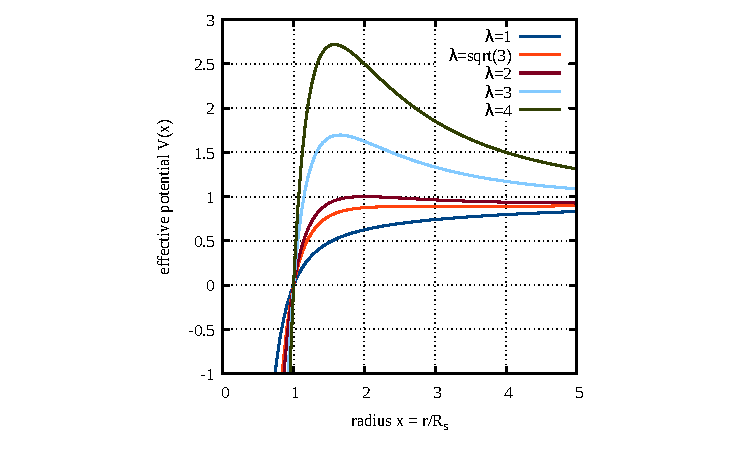
\includegraphics[width=0.48\linewidth]{gfx/fig09-1}
		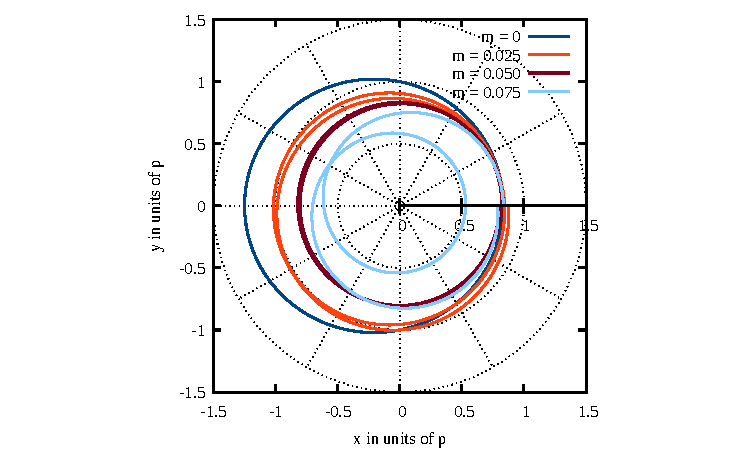
\includegraphics[width=0.48\linewidth]{gfx/fig09-2}
		\caption{\itshape Energy dependent angular-momentum barrier and non-closed elliptic orbits with perihelion shift in Schwarzschild geometry.}
		\label{fig:fig09-1}
	\end{figure}
	
	For $\lambda > \sqrt{3}, V(x=x_+)$ is minimum and $V(x=x_-)$ is maximum. This means that particles with $E\geq 1$ and $L < 2R_s$ will fall unimpededly towards $r=R_s$.\\
	\\
	Thus, In general relativity the situation is different, but only for $r$ sufficiently small. For massless particles there is always a barrier (except
	for $L = 0$, for which the potential vanishes identically), but a sufficiently energetic photon
	will nevertheless go over the barrier and be dragged inexorably down to the center. At the top
	of the barrier there are unstable circular orbits. For massive particles there are once again different regimes depending on the angular
	momentum. Thus $r=6GM$ is the smallest possible radius of a stable
	circular orbit in the Schwarzschild metric. There are also unbound orbits, which come in
	from infinity and turn around, and bound but noncircular ones, which oscillate around the
	stable circular radius. Note that such orbits, which would describe exact conic sections in
	Newtonian gravity, will not do so in GR, although we would have to solve the equation for
	dφ/dt to demonstrate it. Finally, there are orbits which come in from infinity and continue
	all the way in to $r = 0$; this can happen either if the energy is higher than the barrier, or for
	$L < \sqrt{12}GM$, when the barrier goes away entirely.\\
	We have therefore found that the Schwarzschild solution possesses stable circular orbits
	for $r > 6GM$ and unstable circular orbits for $3GM < r < 6GM$. It’s important to remember
	that these are only the geodesics; there is nothing to stop an accelerating particle from
	dipping below $r = 3GM$ and emerging, as long as it stays beyond $r = 2GM$.
	\subsection{Perihelion shift}
	The perihelion is the nearest point in the orbit, while the aphelion is the farthest. One therefore has $u^\prime=0$ and $u=u_+$ at the perihelion, since when $u$ is maximally large, then $r$ is maximally small.
		The precession of perihelia reflects the fact that noncircular orbits are
		not closed ellipses; to a good approximation they are ellipses which precess, describing a
		flower pattern.\\
		\marginpar{The
			observed value is $5601 arcsecs/100 yrs$. However, much of that is due to the precession
			of equinoxes in our geocentric coordinate system; $5025 arcsecs/100 yrs$, to be precise. The
			gravitational perturbations of the other planets contribute an additional $532 arcsecs/100 yrs$,
			leaving $43 arcsecs/100 yrs$ to be explained by GR}
		The treatment of the Kepler problem in CM shows that closed orbits in the Newtonian limit are given by
		\begin{equation}
		u_0 (p) = \frac{1}{p} (1+e \cos \varphi), \quad p=\frac{L^2}{m}=a(1-e^2).
		\end{equation}
		Assuming that the perturbations $3mu^2$ in the e.o.m. is small, we can approximate $3mu \approx 3mu_0$. The solution of the resulting equation is given by particular solutions to driven harmonic oscillator
		\begin{equation}
		u''+u= \left\{\begin{array}{lr}
		A & u_1=A\\
		B \cos \varphi & u_2 = \frac{B}{2} \varphi \sin \varphi\\
		C \cos^2\varphi & u_3 =\frac{C}{2}(1-1/3 \cos^2\varphi)
		\end{array}\right\}
		\end{equation}
		\begin{mybox}{Orbits in the Schwarzschild spacetime}
			Since the unperturbed equation $u''+u=\frac{m}{L^2}$ has the Keplerian solution $u=u_0$, the complete solution is thus the sum
			\begin{align}
				u=u_0+u_1+u_2+u_3&=\frac{1}{p} (1+e \cos \varphi) + \frac{3m}{p^2} \left[1+e \varphi \sin \varphi \right.\nonumber \\
				&\left.  + \frac{e^2}{2} (1-1/3 \cos^2\varphi)\right].
			\end{align}
		\end{mybox}
		$u'|_{\mathrm{perihelion}} = 0= \frac{\md u}{\md \varphi}$ ? $\varphi =0$ is one solution for the perihelion since $u_0$ was constructed like this. What is the next perihelion though after $\varphi = 2 \pi + \delta \varphi$?
		\begin{mybox}{Perihelion shift in the Schwarzschild metric}
			\begin{equation}
			\frac{\md u}{\md \varphi}|_{\varphi = 2 \pi + \delta \varphi} \stackrel{!}{=}0 \; \Rightarrow\; \delta \varphi \approx \frac{3 \pi R_s}{a(1-e^2)} \approx 43''
			\end{equation}
			per century for Mercury's orbit, which reproduces the measurement extremely well.
		\end{mybox}
		\subsubsection{Remark by Weinberg}
		Let $r_+$ and $r_-$ denote the aphelion and perihelion respectively, i.e. $r_{\pm} = (1 \pm e)a$. The change in $\varphi$ as $r$ decreases from $r_+$ to $r_-$ is the same as the change in $\varphi$ as $r$ increases from $r_-$ to $r_+$, so the total change in $\varphi$ per revolution is $2 \abs{\varphi(r_+)-\varphi(r_-)}$. This would equal $2\pi$ if the orbit was a closed ellipse, so in general the orbit precesses in each revolution by an angle
		\begin{equation}
		\Delta \varphi = 2 \abs{\varphi(r_+)-\varphi(r_-)} - 2\pi.
		\end{equation}
		As further remarked under light deflection, we should ask ourselves what the predicted value of $\Delta \varphi$ means. This is not a scattering experiment like the deflection of light by the sun; here we are dealing with an object that never gets out to infinity where the metric is Minkowskian. In practice, these fine points do not really matter, because the precession is cumulative.
		
		
		
		
		
		
		
		\subsection{Light deflection}
		\marginpar{Shapiro delay comes about since light does not travel in a straight line, such that there is a delay of travel time if light passes through a gravitational potential.}
		Repeating the discussion for the effective potential of light rays yields the orbital eq. for light rays in the Schwarzschild space-time:
		\begin{mybox}{E.o.m. of light rays in the Schwarzschild space-time}
			Light rays (null geodesics) in the Schwarzschild space-time follow the orbital equation
			\begin{equation}
			u''+u= 3mu^2.
			\end{equation}
		\end{mybox}
		Again, the correction $3mu^2$ is very small in our solar system and can be treated perturbatively,\\
		$\Rightarrow$ Solution of $u ''+u=0$ is a straight line in polar coordinates $u_0 = \frac{\sin  \varphi}{b}$,
		which is then shifted by the gravitational attraction of the point mass represented by $3mu^2\Rightarrow$ $3mu^2\approx 3mu^2_0$ lowest order perturbative solution
		\begin{equation}
		u=u_0+u_1 = \frac{\sin \varphi}{b} + \frac{3m}{b^2} - \frac{3m}{2 b^2} \left(1- 1/3 \cos^2\varphi\right).
		\end{equation}
		\begin{mybox}{Light deflection in the Schwarzschild metric}
			For $b$ at $\varphi=\frac{\pi}{2}$, we have a light ray coming from the left at large distances.\\
			Deflection angle for light rays is then given by
			\begin{equation}
			\alpha = 2 |\varphi| \approx \frac{4m}{b} = 2 \frac{R_s}{b} \approx 1.74 ''\qquad \mathrm{for \; sun}.
			\end{equation}
		\end{mybox}
		\begin{figure}
			\centering
			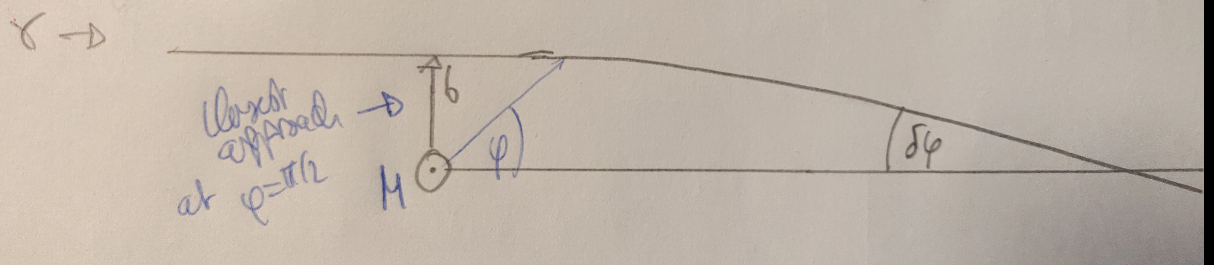
\includegraphics[width=0.7\linewidth]{gfx/LightdeflectionSchwarzschild}
			\caption{\itshape Deflection of light rays due to the gravitational effect of a mass at the centre.}
			\label{fig:lightdeflectionschwarzschild}
		\end{figure}
		
		\subsubsection{Remark by Weinberg}
		\emph{Whenever we obtain a prediction from GR the questions always arises whether the result obtained really refers to an objective physical measurement or whether it has folded into ait arbitrary subjective elements dependent on our choice of coordinate system}. Fortunately, the answer is here quite simple, for this is really a \emph{scattering} experiment. \\
		Another conceptual difficulty that may arise here has to do with our treatment of the photon as a quantum of light moving as would any other particle that happened to have a velocity close to $c$. Actually, no use is being made of QM. The wavelength of light is so small compared with the scale of the solar gravitational field that at any point in this field we can erect a locally inertial coordinate system that covers a huge number of wavelengths. The Principle of Equivalence tells us that in such a coordinate system light behaves as it does in gravitation - free empty space, and since the wavelength is so small, this means that diffraction is negligible and each element of a wave front moves in a straight line at unit velocity.
		
		
		\subsection{Redshift in Schwarzschild Spacetime}
		The gravitational redshift, as we have seen, is another effect which is present in the weak
		field limit, and in fact will be predicted by any theory of gravity which obeys the Principle
		of Equivalence. However, this only applies to small enough regions of spacetime; over larger
		distances, the exact amount of redshift will depend on the metric, and thus on the theory
		under question. It is therefore worth computing the redshift in the Schwarzschild geometry.
		We consider two observers who are not moving on geodesics, but are stuck at fixed spatial
		coordinate values $(r_1 , θ_1 , φ_1 )$ and $(r_2 , θ_2 , φ_2 )$. According to \ref{eq:Schwarzschildmetric}, the proper time of observer
		$i$ will be related to the coordinate time $t$ by
		\begin{equation}
		\frac{\md \tau_i}{\md t} = \sqrt{1-\frac{2 M \mathcal{G}}{r_i}}.
		\end{equation}
		Suppose that the observer $O_1$ emits a light pulse which travels to the observer $O_2$ , such that
		$O_1$ measures the time between two successive crests of the light wave to be $∆τ_1$ . Each crest
		follows the same path to $O_2$ , except that they are separated by a coordinate time $\Delta t$.
		This separation in coordinate time does not change along the photon trajectories, but the
		second observer measures a time between successive crests given by
		\begin{equation}
		\Delta \tau_2 = \sqrt{1-\frac{2 M \mathcal{G}}{r_2}} \Delta t = \sqrt{\frac{1-2 \mG M/r_2}{1-2 \mG M/r_1}} \Delta \tau_1.
		\end{equation}
		Since these intervals $∆τ_i$ measure the proper time between two crests of an electromagnetic
		wave, the observed frequencies will be related by
		\begin{equation}
		\label{eq:redshiftSchwarzschild}
		\frac{\omega_2}{\omega_1} = \frac{\Delta \tau_1}{\Delta \tau_2} \stackrel{r \gg 2 \mG M}{\approx} =1 -\frac{\mG M}{r_1} + \frac{\mG M}{r_2} = 1+\Phi_1 -\Phi_2.
		\end{equation}
		This tells us that the frequency goes down as Φ increases, which happens as we climb out
		of a gravitational field; thus, a redshift.
		
		
		
		
		
		
		
		
		
		
		
		
		
		
		
		
		
		
		
		
		


\newpage
\section{Black Holes}
\subsection{Schwarzschild Black Holes}
A Schwarzschild black hole or \emph{static} black hole is a black hole that has neither electric charge nor angular momentum. A Schwarzschild black hole is described by the Schwarzschild metric, and cannot be distinguished form any other Schwarzschild black hole except by its mass. The Schwarzschild black hole is characterized by a surrounding spherical boundary, called the \emph{event horizon}, which is situated at the Schwarzschild radius. The boundary is not a physical surface, and if a person fell through the event horizon (before being torn apart by tidal forces), they would not notice any physical surface at that position; it is a mathematical surface defining black hole properties. Any non-rotating and non-charged mass that is smaller than its Schwarzschild radius forms a black hole.\\
\\
The \emph{coordinate singularity} at $r=R_s$ divides the Schwarzschild coordinates in two disconnected patches. The exterior Schwarzschild solution with $r>R_s$ is the one that is related to the gravitational fields of stars and planets. The interior Schwarzschild solution with $0 \leq 0 < R_s$, which contains the singularity at $r=0$, is completely separated from the outer patch by the coordinate singularity at $r=R_s$. Using \emph{different coordinates}, one can relate the two patches as the singularity at $r=R_s$ vanishes.\\
The case $r=0$ is different. If one asks that the solution be valid for all $r$ one runs into a \emph{physical singularity}, or \emph{gravitational singularity} at the origin. This singularity is independent of coordinates as one can check from tensor invariants. At $r=0$ the curvature becomes infinite, indicating the presence of a singularity. At this point the metric, and spacetime, itself is no longer well-defined.\\
\\
The solution, i.e. the Schwarzschild black hole, for $r>0$ has bizarre properties. For $r<R_s$, the Schwarzschild radial coordinate $r$ becomes timelike and the time coordinate $t$ becomes spacelike. A curve at constant $r$ is no longer a possible world line of a particle or observer, not even if a force is exerted to try to keep it there. This occurs because spacetime has been curved so much that the direction of cause and effect (the particle's future light cone) points into the singularity. The event horizon represents the point past which no light can no longer escape the gravitational field. Any physical object whose radius $R$ becomes $R \leq R_s$ will undergo gravitational collapse and become a black hole.
\\
\\
How do you check for true singularities ?\\
We have a true singularity when the curvaure becomes infinite. The curvature is
measured by the Riemann tensor, and it is hard to say when a tensor becomes infinite, since
its components are coordinate-dependent. But from the curvature we can construct various
scalar quantities, and since scalars are coordinate-independent it will be meaningful to say
that they become infinite. This simplest such scalar is the Ricci scalar $\mathcal{R} = g_{μν} R\munu$ , but we
can also construct higher-order scalars such as $R\munu R^{μν} $ and
so on. If any of these scalars (not necessarily all of them) go to infinity as we approach some
point, we will regard that point as a singularity of the curvature. We should also check that
the point is not “infinitely far away”; that is, that it can be reached by travelling a finite
distance along a curve. See further under penrose-hawking singularity theorems \ref{subsec:HawkingPenroseSingularity}. E.g. for the Schwarzschild solution we find the true singularity to be at $r=0$ since
\begin{equation}
	\bar{R}^{\mu \nu \sigma \tau}\bar{R}_{\quad \quad \mu \nu  \sigma \tau} =\frac{12 \mathcal{G}^2 M^2}{r^6}.
\end{equation}
\subsubsection{The coordinate singularity at $r=2m$}
Consider an observer freely-falling into the centre of the black hole along a radial orbit (i.e $\dot{\phi} =0 \Rightarrow L=0$). From the e.o.m.
\begin{equation}
	\left(\frac{\md r}{\md \tau}\right)^2 + \left(1-\frac{2m}{r}\right) = E^2,
\end{equation}
one finds that the centre $r=0$ is reached after the \emph{finite proper time} (time measured by a clock moving along the same world line with the observer/test particle)
\begin{equation}
	\tau_0 = \pi \sqrt{\frac{R^3}{8 m} }< \infty.
\end{equation}
This indicates that the observer falls freely from rest at $r=R$ within finite time "through" the singularity at $r=2m$ without encountering a problem.\\
In contrast to this observation, switch to the \emph{coordinate time} $t$ (measured by a stationary clock located infinitely far from the massive body).
The free-fall coordinate time to the centre of a black hole solving the e.o.m. with $t$ instead of $\tau$ and using the tortoise radius, we find
\begin{equation}
	r = 2m+r_0 e^{-\frac{t}{2m}},
\end{equation}
showing that the Schwarzschild radius is only reached after \emph{infinitely} long coordinate time. This is equivalent to the light cone closing up as it approaches the event horizon, i.e. light ray doesn't seem to get to event horizon in coordinate time plane $(r,t)$. Compare to redshift formula \ref{eq:redshiftSchwarzschild}, where this already comes apparent as well, since as in falling astronauts approach $r = 2\mG M$, any
fixed interval $∆τ_1$ of their proper time corresponds to a longer and longer interval $∆τ_2$ from
our point of view, this continues forever. \\
\\
The \emph{tortoise coordinate} is defined as 
\begin{equation}
	r'= r- 2 m \ln{\left|\frac{r}{2m} -1\right|},
\end{equation}
and it approaches $-\infty$  as $r\rightarrow 2m$. When some probe (such as a light ray or an observer) approaches a black hole event horizon, its Schwarzschild time coordinate grows infinite. The outgoing null rays in this coordinate system have an infinite change in $t$ on travelling out from the horizon. The tortoise coordinate is intended to grow infinite at the appropriate rate such as to cancel out this singular behaviour in coordinate systems constructed from it.\\ \\
The increase in the time coordinate to infinity as one approaches the event horizon is why information could never be received back from any probe that is sent through such an event horizon. This is despite the fact that the probe itself can nonetheless travel past the horizon. It is also why the space-time metric of the black hole, when expressed in Schwarzschild coordinates, becomes singular at the horizon - and thereby fails to be able to fully chart the trajectory of an infalling probe.
\\
\\ For radial light rays one finds 
\begin{equation}
	\frac{\md r}{\md t} = \pm \left(1-\frac{2m}{r}\right), 
\end{equation}
suggesting that the light cones become infinitely narrow as $r \rightarrow 2m +$.
\\
\\
Problems on the horizon:\\
These  results appear confusing: While a freely falling observer reaches the Schwarzschild radius and even the centre of the Schwarzschild spacetime after finite proper time, the coordinate time becomes infinite even for reaching the Schwarzschild radius, and the flattening of the light cones as one approaches the Schwarzschild radius is entirely unwanted because causality cannot be assessed when the light cone degenerates to a line.
\\
\\
In coordinate time, the astronaut never reaches $r=R_s \Rightarrow$ shows that something is wrong with $r=2m \Rightarrow$ coordinate singularity.
$G_{\mu \nu}, R^a_b, \mathcal{R}$ are all defined at $r=R_s \Rightarrow$ not a prolem of the spacetime but of our choice of coordinates, i.e. of the Schwarzschild tetrad.

\subsubsection{The Kruskal continuation}
The Kruskal-Szekeres coordinates are a coordinate system for the Schwarzschild geometry for a black hole. These coordinates have the advantage that they cover the entire spacetime manifold of the maximally extended Schwarzschild solution and are well-behaved everywhere outside the physical singularity. These are coordinates in which the light-cone stays Minkowskian like $X$ all the time by construction, independent of motion.
\marginpar{The light cone itself is invariant, but in some coordinates you may not see this properly.}
\begin{mybox}{Kruskal coordinates}
	The Kruskal coordinates $(t,r) \mapsto (v,u)$ are constructed such that the light cones remain the same everywhere:
	\begin{equation}
		g = -f^2(u,v) (\md v^2 -\md u^2) + r^2 \md \Omega^2,
	\end{equation}
	such that for a light ray
	\begin{equation}
		\md s= 0 \quad \Rightarrow \quad \left(\frac{\md u}{\md v}\right)^2 =1 \; \Leftrightarrow \; \mathrm{Minkowskian \; lightcone.}
	\end{equation}
	Solving the resulting equations and applying physical boundary conditions of our Schwarzschild spacetime yields
	\begin{align}
		u &= \sqrt{\frac{r}{2m} -1 } e^{\frac{r}{4m}} \cosh{\frac{t}{4m}}, \\
		v &= \sqrt{\frac{r}{2m} -1} e^{\frac{r}{4m}} \sinh{\frac{t}{4m}}, \\
		f^2 &= \frac{32 m^3}{r} e^{- \frac{r}{2m}}.
	\end{align}
\end{mybox}
Coordinate transformation recipe:\\
\begin{equation}
	(t,r,\vartheta\varphi) \mapsto (v,u,\vartheta,\varphi) \, \Rightarrow \, (\mathcal{J}^{\alpha}_{\beta}) = \begin{pmatrix}
	\partial_t v & \partial_tu & 0&0\\
	\partial_r v & \partial_r u &0&0 \\
	0&0&1&0\\
	0&0&0&1\\
	\end{pmatrix}
\end{equation}
with $(\tilde{\mathcal{J}} ) = \frac{\partial(v,u)}{\partial (t,r)}$. Then the new metric reads
\begin{equation}
	\tilde{g} = \mathrm{diag}\left(-f^2,f^2,r^2,r^2 \sin^2\vartheta\right),
\end{equation}
and is transformed into the metric in original coordinates by

\begin{equation}
	g = \mathcal{J} \tilde{g} \mathcal{J}^T.
\end{equation}

\subsubsection{Physical meaning of the Kruskal coordinates}
We can maximally extend the Kruskal coordinates to $r \in [0,\infty)$ by $\sqrt{\frac{r}{2m} -1} \mapsto\sqrt{|\frac{r}{2m} -1|}$ due to many sign choices along the way of the derivation.\\
A static observer inside the Schwarzschild radius is also not possible anymore, since the radial-coordinate becomes time-like at $r<R_s \Rightarrow$ global Killing vector field is lost.\\
\begin{mybox}{Non-static interior of the Schwarzschild horizon}
	The Killing vector field $K=\partial_t$ for the Schwarzschild spacetime outside $r=2m$ becomes space-like for $r<2m$, which means that the spacetime cannot be static any more inside the Schwarzschild radius.
\end{mybox}
Domains of the the Kruskal spacetime:\\
Region $I$ and $III$ are asymptotically flat regions, $II$ is the interior of the black hole. Once
anything travels from region $I$ into $II$, it can never return. In fact, every future-directed path
in region $II$ ends up hitting the singularity at $r = 0$; once you enter the event horizon, you are
utterly doomed. This is worth stressing; not only can you not escape back to region $I$, you
cannot even stop yourself from moving in the direction of decreasing $r$, since this is simply
the timelike direction. Thus you can no more stop moving
toward the singularity than you can stop getting older. Since proper time is maximized along
a geodesic, you will live the longest if you don’t struggle, but just relax as you approach
the singularity. Not that you will have long to relax. (Nor that the voyage will be very
relaxing; as you approach the singularity the tidal forces become infinite. As you fall toward
the singularity your feet and head will be pulled apart from each other, while your torso
is squeezed to infinitesimal thinness. \\
\\
$IV$ is a white hole.
There is a singularity in the past, out of which
the universe appears to spring. The boundary of region $III$ is sometimes called the \emph{past event horizon}, while the boundary of region $II$ is called the \emph{future event horizon}.\\
The bold hyperbolae in regions $II$ and $IV$ are the singularities. Region $IV$,
meanwhile, cannot be reached from our region $I$ either forward or backward in time (nor can
anybody from over there reach us). It is another asymptotically flat region of spacetime, a
mirror image of ours. It can be thought of as being connected to region I by a “wormhole,” a
neck-like configuration joining two distinct regions. The dashed diagonals through the origin are the event horizons. The origin (really a 2-sphere with angular coordinates suppressed) is the throat of a non-traversable wormhole joining the separate "universes" $I$ and $III$. Radial light rays remain $45$ degree diagonal lines on the Kruskal-Szekeres diagram. The thin hyperbolae are lines of constant Schwarzschild $r$ coordinate, and the thin radial rays are lines of constant $t$. You can see how the event horizon becomes a coordinate singularity where $r$ and $t$ switch roles, i.e. at the dashed diagonal lines they switch roles and there also the event horizon is.\\
The exterior of the Schwarzschild radius corresponds to the domain $u>0, |v| < u$, and its interior is bounded in the $(u,v)$-plane by the lines $u>0,|v| =u$, and $v^2- u^2 =1$, compare \ref{fig:Schwarzschildbh}. ON figure \ref{fig:Schwarzschildbh}:
\begin{enumerate}
	\item hyperbolic lines $=r$ constant,
	\item straight lines $=t$ constant at $r=2m$. 
	\item Lines  of constant $r,t$ meet $\Rightarrow$ reflects that coordinate time $t \rightarrow \infty$ at $r=2m$
	\item (I) Everything outside $r>2m$, our world
	\item (II) everything inside $r<2m$, dark blue line represents the true singularity
	\item Beyond green bold line is "white hole". Can't keep anything for itself, light in IV has to escape. White hole would thus violate thermodynamics, the $2^{nd}$ coverage of the Kruskal coordinates is thus \emph{not physical}.
\end{enumerate}
\begin{figure}[h]
	\label{fig:Schwarzschildbh}
	\centering
	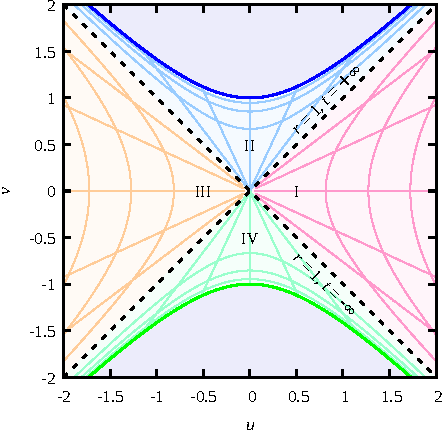
\includegraphics[width=0.8\textwidth]{gfx/fig10-2.pdf}
	\caption{\itshape Schwarzschild black hole in Kruskal coordinates, regions I \& II are double-covered by regions III \& IV.}
\end{figure}
Radial light rays propagate according to $\md s^2 =0$ or $\md v = \md u$, i.e. they are straight diagonal lines in the $(u,v)$ plane. This shows that light rays can propagate freely into the region $r<2m$, but there is no causal connection from within $r<2m$ to the outside.
\begin{mybox}{Radial light rays in Kruskal spacetime}
	The light cones are Minkowskian everywhere by construction of the Kruskal coordinates, since 
	\begin{equation*}
		\md s^2 =  0 \quad \Leftrightarrow \quad (\md u^2 - \md v^2 ) = 0 \quad \Leftrightarrow \quad \md u =\md v.
	\end{equation*}
	Radial light rays propagate according to $\md v = \md u$, i.e. they are straight diagonal lines in the
	$(u, v)$-plane. Thus, light rays can propagate freely into the region $II$ with $r < 2m$ from the outside
	region $I$, but there is no causal connection from within region $II$ with $r < 2m$ to the outside
	region I.
\end{mybox}
Now if you draw a worldline from region I going into region II it becomes obvious that it crosses the horizon in finite proper time and, more importantly, the past light-cone of the event where it hits the singularity cannot possibly contain the whole spacetime. So the short answer to the question is no, someone falling into a black hole does not see the end of the universe. Compare also
\begin{figure}[h!]
	\centering
	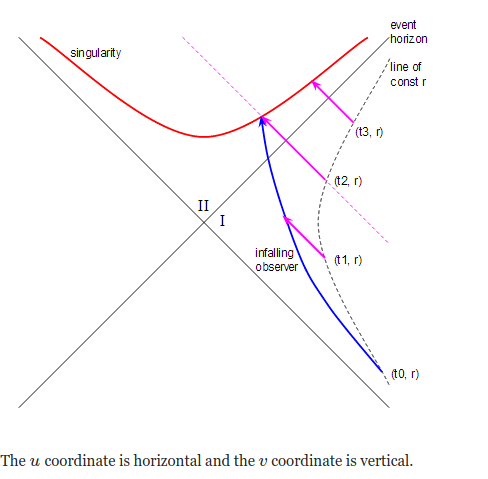
\includegraphics[width=0.7\linewidth]{gfx/kruskalszekerescoordInfallingObs}
	\caption{}
	\label{fig:kruskalszekerescoordinfallingobs}
\end{figure}
The problem with these coordinates is that they are highly unintuitive. A displacement in $u$ or $v$ doesn't correspond to any simple physical quantity, unlike a displacement in the usual radial coordinate $r$ or time coordinate $t$. Nevertheless the KS coordinates simplify things drastically as follows:
\\
In these coordinates constant $r$ is a hyperbola as shown by the dashed line. The event horizon is the solid $45°$ line. You can sort of think as $t$ increasing as you move up - it does, though not in a linear way. The singularity is the red hyperbola (this is a spacetime diagram remember, so the singularity is a curve not a point). The region I've labelled $I$ is the exterior of the black hole and the region I've labelled $II$ is the region inside the event horizon. Ignore the region of the diagram to the bottom left as it isn't relevant to my question.
\\
Finally, the key feature that makes it possible to answer my question is that all radial ingoing light rays are straight $45°$ lines running from bottom right to top left. I've drawn several such light rays as magenta lines.\\

Now we can answer my question. We start with a rocket hovering at a constant distance away from the black hole, which is represented by the black dashed hyperbola of constant $r$ (as I mentioned above you can sort of think about time increasing as you move up). At time $t0$ our observer leaves the rocket and starts falling towards the black hole. The blue line shows the trajectory followed by the observer. The observer hits the singularity at the point where the blue and red lines meet.

At time $t1$ the rocket shines a light ray at the infalling observer. The light ray, travelling at $45°$, reaches the observer before they cross the event horizon - so far so good. At time $t2$ the rocket shines a second light ray at the observer, and this light ray reaches the observer just as they hit the singularity. At time $t3$ the rocket shines a third light ray into the black hole, but this doesn't reach the observer because the observer has already hit the singularity and no longer exists. That means the observer never sees the light ray released at time $t3$. The observer sees any light ray released between $t0$ and $t2$, but doesn't see any light ray released after $t2$. So the dashed magenta line marks the boundary between light rays the observer can see and ones they can't.\\

And there is the answer to my question. The observer does not see the end of the universe because the last light ray they see is the one released at time $t2$.




















\subsubsection{Eddington-Finkelstein coordinates}
In general relativity, Eddington–Finkelstein coordinates are a pair of coordinate systems for a Schwarzschild geometry (i.e. a spherically symmetric black hole) which are adapted to radial null geodesics. Null geodesics are the worldlines of photons; radial ones are those that are moving directly towards or away from the central mass. In these coordinate systems, outward (inward) traveling radial light rays (which each follow a null geodesic) define the surfaces of constant "time", while the radial coordinate is the usual area coordinate so that the surfaces of rotation symmetry have an area of $4\pi r^2$. One advantage of this coordinate system is that it shows that the apparent singularity at the Schwarzschild radius is only a coordinate singularity and is not a true physical singularity. \\
\\
We perform the coordinate transform to the tortoise time
\begin{equation}
	(r,\vartheta,\varphi), t \mapsto t', \; t = t' - 2 m \ln{\left[\pm \frac{r}{2m} \mp 1 \right]} \; \Rightarrow \; \left\{\begin{array}{lr}
	\mathrm{upper \, sign}, & \text{for } r\geq 2m\\
	\mathrm{lower \, sign}, & \text{for } r < 2m\\
	\end{array}\right\},
\end{equation}
which yields the  line element in Eddington-Finkelstein coordinates
\todo{Insert line element here}
where the metric acquires off-diagonal elements such that it no longer
depends on $t'$ and $r$ separately.\\
\\
\begin{mybox}{Light cones in Eddington-Finkelstein coordinates}
	For radial light rays we have $\md \Omega^2 = 0, \md s =0$ implying that $\md r = - \md t'$.
	Light cones in Eddington-Finkelstein coordinates are thus defined either by
	\begin{equation}
	\label{eq:edfinklightcone}
	\frac{\md r}{\md t'} = -1 \; \Rightarrow r = -t'+ const.
	\end{equation}
or by
\begin{equation}
	\frac{\md r}{\md t'} = \frac{r-2m}{r+2m}
\end{equation}
This shows that $\md r /\md t' \rightarrow −1$ for $r \rightarrow0, \md r/\md t' = 0$ for $r = 2m$, and
	$\md r/\md t'= 1$ for $r \rightarrow \infty$. Due to the vanishing derivative of $r$ with respect
	to $t'$ at $r = 2m$, geodesics cannot cross the Schwarzschild radius from
	inside, but they can from outside because of \ref{eq:edfinklightcone}.\\
	Thus, at at $r=R_s$, the light cone changes as $X\mapsto + \Rightarrow$ light ray doesn't propagate any more at $r=R_s$ in the sense that they wrap around the black hole infinitely. As $r \rightarrow 2m + \rightarrow 0+$, causality hence changes.
\end{mybox}

\todo{Include figure of eddington finkelstein lightcones}
\begin{figure}[h!]
	\centering
	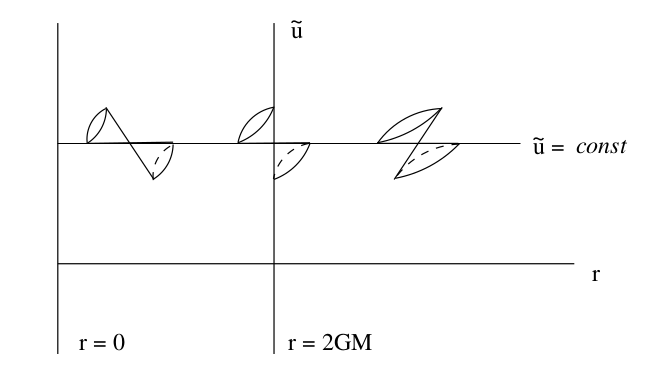
\includegraphics[width=0.7\linewidth]{gfx/eddingtonFinkelsteinLightcone}
	\caption{}
	\label{fig:eddingtonfinkelsteinlightcone}
\end{figure}

We can therefore see what has happened: in this coordinate system the light cones remain
well-behaved at $r = 2\mG M$, and this surface is at a finite coordinate value. There is no
problem in tracing the paths of null or timelike particles past the surface. On the other
hand, something interesting is certainly going on. Although the light cones don’t close up,
they do tilt over, such that for $r < 2GM$ all future-directed paths are in the direction of
decreasing $r$.\\
The surface $r = 2\mG M$, while being locally perfectly regular, globally functions as a point
of no return — once a test particle dips below it, it can never come back. For this reason
$r = 2\mG M$ is known as the \emph{event horizon}; no event at $r ≤ 2\mG M$ can influence any other event at $r > 2\mG M$. Notice that the event horizon is a null surface, not a timelike one. Notice
also that since nothing can escape the event horizon, it is impossible for us to “see inside”
— thus the name \emph{black hole}












.
\subsubsection{Redshift approaching the Schwarzschild radius}
Suppose a light-emitting source (e.g. an astronaut with a torch) is falling
towards a (Schwarzschild) black hole, what does a distant observer at rest far away from the black hole see?
The astronauts' and observers' four velocity $v,u$ define local time directions. The local frequency projected out depends on the frame of either observer or astronaut. The redshift of the light from the
torch as seen by the observer is
\begin{equation}
	1+z = \frac{\nu_{em}}{\nu_{obs}} = \frac{\langle k,v\rangle}{\langle k,u\rangle}.
\end{equation}
The calculation is performed with the used of the retarded time $\md t_{ret} = \md t - \frac{\md r}{1-\frac{2m}{r}}$, which runs on the lightcone from astronaut to observer. Radial light rays in this coordinate cannot have a time dependence : $k \propto \partial_r$. Be careful when you read of metric components from the line element, since in the line element you get off-diagonal contributions twice ! Take half their contribution, since 
\begin{equation*}
	(\md x)^T g(\md x) = \md s^2 = (\md x)^T \begin{pmatrix}
	g_{00} &g_{ij}\\
	g_{ji} & g_{aa} \\
	\end{pmatrix}
	(\md x),
	\qquad g_{ij} \dot{x}^i \dot{x}^j + g_{ji} \dot{x}^j \dot{x}^i=2 g_{ij} \dot{x}^i \dot{x}^j.
\end{equation*}
\\
A calculation shows that the astronaut’s redshift
\begin{equation}
	1+z = e^{\frac{t}{2m} -2}
\end{equation}
grows exponentially to infinity as she approaches the Schwarzschild radius. This resolves the apparent contradiction that, while the astronaut has
long reached the singularity as measured by her own watch, the distant
observer never even sees her reach the Schwarzschild radius: The signal
of the astronaut’s passing the Schwarzschild radius is infinitely delayed
and thus never reaches the distant observer.\\
The astronaut is in free fall, there is no gravity. She reaches $r=0$ instantly without delay. Observer never sees astronaut arriving at $r=R_s$, since the signal of astronaut is infinitely delayed as it is infinitely redshifted and since she reaches $r=R_s$ only at $t= \infty$ from our POV.
Paradox is not there. Signal simply never reaches the observer, even though the astronaut already entered $r< R_s$. For us it only occurs at $t=\infty$ as seen from our watch outside of black hole.
\subsubsection{Penrose (or Carter-Penrose,or conformal) diagram  - TO DO}
The idea is to do a conformal transformation which brings the entire
manifold onto a compact region such that we can fit the spacetime on a piece of paper, c.f. p. 192 caroll.\\
\\
Once again the Penrose diagrams for these spacetimes don’t really tell us anything we
didn’t already know; their usefulness will become evident when we consider more general
black holes. In principle there could be a wide variety of types of black holes, depending on
the process by which they were formed. Surprisingly, however, this turns out not to be the
case; no matter how a black hole is formed, it settles down (fairly quickly) into a state which
is characterized only by the mass, charge, and angular momentum. This property, which
must be demonstrated individually for the various types of fields which one might imagine
go into the construction of the hole, is often stated as “\emph{black holes have no hair}.”
\newpage

\subsection{Charged, Rotating Black Holes}
\subsubsection{The Reissner-Nordström solution}
The Reissner–Nordström metric is a static solution to the Einstein field equations, which corresponds to the gravitational field of a charged, non-rotating, spherically symmetric body of mass M. Now we are no longer in vacuum, since the hole will have a non-zero electromagnetic
field, which in turn acts as a source of energy-momentum.First, we consider a static, axially-symmetric solution of Einstein’s
equations in the presence of an electromagnetic charge $q$ at the origin of
the Schwarzschild coordinates, i.e. at $ r = 0$. The electromagnetic field
will then also be static and axially symmetric. The axial symmetry implies that the charge won't move, hence no $B$-field is generated and the spatial symmetry of the Schwarzschild solution is retained. We can therefore simply add the energy-momentum tensor due to the presence of the charge to the vacuum Einstein field equations for the Schwarzschild black hole. Due to the radial symmetry, the only non-vanishing component of the Faraday form is $F_{01}  = \frac{q}{r^2}$, such that the energy-momentum tensor of the electromagnetic field is readily available in the Schwarzschild tetrad. Note that the Faraday form suffices the homogeneous and inhomogeneous (in vacuum) Maxwell equations by construction.
Gravity coupled to the electromagnetic field is described by the Einstein-Maxwell
action
\begin{equation}
	S= \frac{1}{16 \pi \mG} \int \md^4 x \sqrt{-g} \left[\mathcal{R}-F\munu F^{\mu \nu} \right]
\end{equation}
where $F\munu = ∇_μ A_ν − ∇_ν A_μ$ and $A_μ$ is the electromagnetic (four-)potential. The
normalisation of the Maxwell term is such that the Coulomb force between
two charges $Q_1$ and $Q_2$ separated by a (large enough) distance $r$ is $\mG|Q_1 Q_2 |/r^2$ . This
corresponds to geometrised units of charge.\\
The field equations in this case are both
Einstein’s equations and Maxwell’s equations, thus the equations of motion derived from the variation of the Einstein-Maxwell
action are
\begin{align}
	G\munu &= 2 \left[F_{\mu \lambda} F^\lambda_{\,\; \nu} - \frac{1}{4} g\munu F_{\rho \sigma} F^{\rho \sigma} \right]\\
	\nabla_\mu F^{\mu \nu} &=0.
\end{align}
The two sets are coupled together, since the electromagnetic field strength tensor enters
Einstein’s equations through the energy-momentum tensor, while the metric enters explicitly
\marginpar{By a theorem analogous to Birkhoff’s theorem, the Reissner-Nordström solution is the unique spherically
	symmetric solution to the Einstein-Maxwell equations}
into Maxwell’s equations. They admit the spherically symmetry solution known as the Reissner-Nordström solution.
\begin{mybox}{Reissner-Nordström solution}
	Defining
	\begin{equation}
		\Delta := r^2 -2mr + Q^2, \qquad Q:= \frac{\mG q^2}{c^4}.
	\end{equation}
	we thus obtain the line element for the metric of a charged Schwarzschild black hole,
	\begin{equation}
		\md s^2 = \frac{- \Delta}{r^2} \md t^2 + \frac{r^2 \md r^2}{\Delta} + r^2 \md \Omega^2.
	\end{equation}
	This is the \emph{Reissner-Nordström solution}.
\end{mybox}
Of course, for $q = 0$, the Reissner-Nordström solution returns to the
Schwarzschild solution.
\todo{homework: set up $\mathcal{L}$, identify $V(r)$ and check what happens}
Although charged black holes with $r_q \ll  r$, with $r^2_q := \frac{\mathcal{G} q^2}{c^4}$ is a characteristic length scale, are similar to the Schwarzschild black hole, they have two horizons: the event horizon and an internal \emph{Cauchy horizon}. In physics, a Cauchy horizon is a light-like boundary of the domain of validity of a Cauchy problem (a particular boundary value problem of the theory of partial differential equations). One side of the horizon contains closed space-like geodesics and the other side contains closed time-like geodesics. The simplest example is the internal horizon of a Reissner–Nordström black hole. As with the Schwarzschild metric, the event horizons for the spacetime are located where the metric component $g^{rr}$ diverges, i.e. the equivalent to $r=2m$; that is, where
\begin{equation}
	0 =  \Delta= \frac{1}{g^{rr}} = 1- \frac{r_s}{r} + \frac{r^2_q}{r^2}, \quad r_{\pm} = \frac{1}{2} \left( r_s \pm   \sqrt{r^2_s - 4r^2_q}\right).
\end{equation}
These concentric event horizons become degenerate for $2 r_q = r_s$, which corresponds to an extremal black hole. Black holes with $2r_q > r_s$ can not exist in nature because if the charge is greater than the mass there can be no physical event horizon (the term under the square root becomes negative). Objects with a charge greater than their mass can exist in nature, but they can not collapse down to a black hole, and if they could, they would display a naked singularity. The nakedness of the singularity offends our sense of decency, as well as the \emph{cosmic censorship conjecture}, which roughly states that the gravitational collapse of physical matter
configurations will never produce a naked singularity.
\\
\\
On the true event horizons at $\Delta = (r_+ -r)(r_-r)$:\\
The singularity at $r = 0$ is a timelike line (not
a spacelike surface as in Schwarzschild). If you are an observer falling into the black hole
from far away, $r_+$ is just like $2\mG M$ in the Schwarzschild metric; at this radius $r$ switches
from being a spacelike coordinate to a timelike coordinate, and you necessarily move in the
direction of decreasing $r$. Witnesses outside the black hole also see the same phenomena
that they would outside an uncharged hole — the infalling observer is seen to move more
and more slowly, and is increasingly redshifted.\\
But the inevitable fall from $r_+$ to ever-decreasing radii only lasts until you reach the null
surface $r = r_−$ , where $r$ switches back to being a spacelike coordinate and the motion in the
direction of decreasing $r$ can be arrested. Therefore you do not have to hit the singularity
at $r = 0$; this is to be expected, since $r = 0$ is a timelike line (and therefore not necessarily
in your future). In fact you can choose either to continue on to $r = 0$, or begin to move
in the direction of increasing $r$ back through the null surface at $r = r_−$ . Then $r$ will once
again be a timelike coordinate, but with reversed orientation; you are forced to move in the
direction of increasing $r$. You will eventually be spit out past $r = r_+$ once more, which is
like emerging from a white hole into the rest of the universe. From here you can choose to
go back into the black hole — this time, a different hole than the one you entered in the
first place — and repeat the voyage as many times as you like.\\
How much of this is science, as opposed to science fiction? Probably not much. If you
think about the world as seen from an observer inside the black hole who is about to cross the
event horizon at $r_−$ , you will notice that they can look back in time to see the entire history
of the external (asymptotically flat) universe, at least as seen from the black hole. But they
see this (infinitely long) history in a finite amount of their proper time — thus, any signal
that gets to them as they approach $r_−$ is infinitely blueshifted.

\subsubsection{Kerr-Newmann solution}
The Kerr–Newman metric is the most general asymptotically flat, stationary solution of the Einstein equations in general relativity that describes the spacetime geometry in the region surrounding an electrically charged, rotating mass. It generalizes the Kerr metric (the Kerr metric or Kerr geometry describes the geometry of empty spacetime around a rotating uncharged axially-symmetric black hole with a quasispherical event horizon. ) by taking into account the field energy of an electromagnetic field, in addition to describing rotation. It is one of a large number of various different electrovacuum solutions, that is, of solutions to the Einstein equations which account for the field energy of an electromagnetic field. Such solutions do not include any electric charges other than that associated with the gravitational field, and are thus termed vacuum solutions. When a black hole is rotating, there is no analogue of Birkhoff’s theorem. This
means that, during gravitational collapse with rotating matter, we cannot use the
same reasoning as in the spherically symmetric case to argue that, on the surface of
the collapsing matter, the metric should be of the form given above. All we can say
is that, after enough time has passed and matter and spacetime have “settled down”
to equilibrium, they will be described by the Kerr-Newman solution.\\
\\
In presence of angular momentum, we expect the spherical symmetry
of the Schwarzschild solution to be broken. Instead, we expect that
the solution must be \emph{axisymmetric}, with the axis fixed by the angular
momentum. Moreover, we seek to find a stationary solution.
Then, the group $\mR \times SO(2)$ must be an isometry of the metric, where
$\mR$ represents the stationariness (can not be static since it is rotating) and $SO(2)$ the (two-dimensional) rotations
about the symmetry axis. Expressing these symmetries, there must be a
time-like Killing vector field $k$ and another Killing vector field $m$ which
is tangential to the orbits of $SO(2)$. We therefore have one Killing field for the stationariness and one for the axial symmetry.
These two Killing vector fields span the tangent spaces of the two-dimensional sub manifolds which are the orbits of $\mR \times SO(2)$, i.e. cylinders.
We can choose adapted coordinates $t$ and $\varphi$ such that $k = \partial_t$ and $m = \partial_{\varphi}$. The fact that $k,m$ are Killing vectors is equivalent to the fact that the metric coefficients do not depend on $t$ and $\varphi$.
\marginpar{The Kerr spacetime possesses a Killing tensor, c.f. Caroll p.208}
Then, the metric $^{(4)} g$ of four-dimensional space-time can be decomposed as
\begin{equation}
	^{(4)} g = g_{ab} (x^i) \md x^a \otimes \md x^b + g_{ij} (x^k) \md x^i \otimes \md x^j,
\end{equation}
where indices $a,b=0,1$ indicate the coordinates on the orbits of
$\mR \times SO(2)$, and indices $i, j, k = 2, 3$ the others. Note that, due to the
symmetry imposed, the remaining metric coefficients can only depend
on the coordinates $x^i$ .\\
\\
A stationary, axi-symmetric space-time $(M, g)$ can thus be foliated into
$M =  \Sigma \times \Gamma$, where $\Sigma \cong \mR \times SO(2)$ is diffeomorphic to the orbits of $\mR \times SO(2)$, and
the metric coefficients in adapted coordinates can only depend on the coordinates of $\Gamma$.
\\
\begin{figure}
		\centering
		\includegraphics[width=0.7\textwidth]{gfx/KerrNewmannSpacetime.jpg}
		\caption{\itshape Foliation of spacetime for the Kerr-Newmann solution.}
\end{figure}
We write
\begin{equation}
^{(4)}g = \sigma + g,
\end{equation}
where 
\begin{equation}
	\sigma = \sigma_{ab} (x^i) \md x^a \otimes \md x^b .
\end{equation}
The coefficients $\sigma_{ab}$ are scalar products of the two Killing vector fields $k$ and $m$,
\begin{equation}
	(\sigma_{ab}) = 
	\begin{pmatrix}
	-\langle k,k \rangle & \langle k, m \rangle\\
	\langle k,m \rangle & \langle m, m\rangle\\
	\end{pmatrix}, \quad \rho := \sqrt{-\det{\sigma}}.
\end{equation}\\
\\
Define the following auxilliary quantities
\begin{align*}
	\Delta & := r^2- 2mr + Q^2 +a^2, \quad \rho^2 := r^2 +a^2 \cos^2 \vartheta ,\\
	\Sigma^2 &:= (r^2+a^2)^2 -a^2 \Delta \sin^2 \vartheta, \\
	Q^2 &:= \frac{\mathcal{G}q^2}{c^4}, \quad a:= \frac{L}{Mc} = \frac{\mathcal{G}L}{m c^3}, \; [a]=[Q]=\mathrm{length}.	
\end{align*}
Note that $L$ and thus also $a$ describes the angular momentum of the rotating black hole.
\begin{mybox}{Kerr-Newmann solution}
	With these definitions, we can write the coefficients of the metric for a
	charged, rotating black hole in the form
	\begin{align}
		g_{tt} &=-1 + \frac{2mr -Q^2}{\rho^2} = g_{00, \mathrm{Schwarzschild}} |_{L,Q =0}\\
		g_{t\varphi} &= -\frac{2mr-Q^2}{\rho^2}  \sin^2\vartheta \\
		g_{\varphi \varphi} &= \frac{\Sigma^2}{\rho^2} \sin^2\vartheta, \quad g_{rr} = \frac{\rho^2}{\Delta}, \quad g_{\vartheta \vartheta} = \rho^2.
	\end{align}
Notice how $t,\varphi$ are coupled here in $g_{t \varphi}$, since we chose adapted coordinates $(t,\varphi)$ and since the black hole is rotating. They will have to point into direction of the Killing vector fields $k,m$ together, i.e. they describe screws in the cylinder.
\begin{align}
 g_{\mathrm{Kerr-Newmann}} |_{Q=0} &= g_{\mathrm{Kerr}}, \\
  g_{\mathrm{Kerr-Newmann}} |_{L=0} &= g_{\mathrm{Reissner-Nordström}}.
\end{align}
\end{mybox}

Any Kerr–Newman source has its rotation axis aligned with its magnetic axis. Thus, a Kerr–Newman source is different from commonly observed astronomical bodies, for which there is a substantial angle between the rotation axis and the magnetic moment. Specifically, neither the Sun, nor any of the planets in the Solar system have magnetic fields aligned with the spin axis. Thus, while the Kerr solution describes the gravitational field of the Sun and planets, the magnetic fields arise by a different process.
\begin{mybox}{Kerr metric}
The line element of the Kerr metric for an uncharged rotating black hole with angular momentum $\tilde{L}$
is given by
\begin{align}
	\label{eq:kerrmetric}
	\md s^2&= -\left(1-\frac{2mr}{\rho^2}\right) \md t^2 - \frac{4mra}{\rho^2} \sin^2 \vartheta \md t \md \varphi + \frac{\rho^2}{\Delta}\md r^2\nonumber \\
	& + ρ^2 \md\vartheta^2 + \frac{\Sigma^2}{\rho^2} sin^2 \vartheta \md φ^2,
\end{align}
with
\begin{align}
	ρ^2 &≡ r^2 + a^2 \cos^2 \vartheta,\;	∆ ≡ r^2 − 2mr + a^2 ,\nonumber \\
	Σ^2 &≡ (r^2 + a^2)^2 − a^2 ∆ \sin^2 \vartheta, \; a=\frac{\mG \tilde{L}}{mc^3}.\nonumber
\end{align}
\end{mybox}
A note on the singularities in the KN-solution:
\begin{enumerate}
	\item One is $\Delta=0$, the resulting equation has three distinct cases where the only physical one is $\mG^2 M^2 > a^2$, which has the two null surfaces (which turn out to be event horizons)
	\begin{equation}
		r_{\pm} = \mG M \pm \sqrt{\mG^2 M^2-a^2}.
	\end{equation}
	\item Besides the event horizons at $r_±$ , the Kerr solution also features an additional surface
	of interest. Recall that in the spherically symmetric solutions, the “timelike” Killing vector
	$k^μ = ∂_t$ actually became null on the (outer) event horizon, and spacelike inside. Analogously for Kerr yields
	 \begin{equation}
	 k_\mu k^\mu = −\frac{1}{\rho^2}	(∆ − a^2 \sin^2 θ).
	 \end{equation}
	 This does not vanish at the outer event horizon; in fact, at $r = r_+$ (where $∆ = 0$), we have
\begin{equation}
		k^2 = \frac{a^2}{\rho^2} \sin^2\theta \geq 0.
\end{equation}	
	So the Killing vector is already spacelike at the outer horizon, except at the north and south
	poles ($θ = 0$) where it is null.\\
	The locus of points where $k^\mu k_\mu = 0$ is known as the \emph{Killing
	horizon}, and is given by
\begin{equation}
	(r − \mG M)^2 = \mG^2 M^2 − a^2 \cos^2 θ ,
\end{equation}
while the outer event horizon is given by
\begin{equation}
	(r_+ − \mG M)^2 = \mG^2 M^2 − a^2.
\end{equation}
There is thus a region in between these two surfaces, known as the \emph{ergosphere}. Inside the
ergosphere, you must move in the direction of the rotation of the black hole (the $\phi$ direction);
however, you can still move towards or away from the event horizon (and there is no trouble exiting
the ergosphere).
\item True curvature singularity occurs in this spacetime at
\begin{equation}
	\rho=0 \quad \Leftrightarrow \quad r=0 \, \& \, \theta=\frac{\pi}{2}.
\end{equation}
This seems like a funny result, but remember that $r = 0$ is not a point in space, but a disk;
the set of points $r = 0, θ = π/2$ is actually the ring at the edge of this disk. The rotation
has “softened” the Schwarzschild singularity, spreading it out over a ring.\\
The region near the ring singularity has additional pathologies: closed timelike curves. Since these paths are closed, they are obviously closed time-like curves (c.f. CTC on Wikipedia). You can therefore meet yourself in the past, with all that entails.
\end{enumerate}
\vspace{1.5cm}
The vector potential of the rotating,
charged black hole is given by the 1-form
\begin{equation}
	A = - \frac{q r}{\rho^2} (\md t - a \sin^2\vartheta \md \phi), \quad F=\md A.
\end{equation} 
In the limit of large $r$, i.e. $a \ll r$, the
electric field thus becomes that of a point charge q at the origin, and the
magnetic field has a characteristic dipolar structure. From the non-vanishing (magnetic) field components
\begin{equation}
	E_r = F(e_r,e_t)=\frac{q}{r^2}, \; B_r = F(e_{\vartheta}, e_{\varphi}) = \frac{2qa}{r^3} \cos \vartheta,\; B_{\vartheta} = F(e_{\vartheta}, e_r) = \frac{q a}{r^3} \sin \vartheta,
	\end{equation}
	 one can read of the magnetic dipole moment for a sphere.
	 \begin{mybox}{Magnetic dipole moment of a charged, rotating black hole}
	 The magnetic dipole moment of a charged, rotating black holes has the
	 modulus
\begin{equation}
	\mu = qa =2 \frac{qL}{2 Mc},
\end{equation}
	 showing that its gyromagnetic moment is g = 2.
	 \end{mybox}
 \vspace{1cm}
 Interesting properties:
 \begin{enumerate}
\item 	Since the metric coefficient satisfy the following relations w.r.t. to the symmetries of the system expressed by the two Killing vector fields in adapted coordinates
	\begin{equation}
	g_{tt} = \langle k,k\rangle,\quad g_{\varphi,t} = \langle m, k\rangle, \quad g_{\varphi \varphi} = \langle m,m \rangle,
	\end{equation}
	they have an invariant meaning, which will be discussed in the following. Consider an observer on a circular orbit in equatorial plane, i.e. $\vec{L}_{BH} \parallel \vec{L}_O$, of the black hole orbiting with a uniform angular velocity $\omega$ (as seen by a distant observer). Since the black hole is rotating, the rotational direction, whether observer rotates with or against the black hole, matters a lot due to the \emph{drag of spacetime} induced by the black hole. At which radius does the four velocity of the observer become light-like $u =c?, \Leftrightarrow \langle u, u \rangle =0?$
	\begin{equation}
		\Leftrightarrow w_{\pm} = \Omega \pm \sqrt{\Omega^2 - \frac{g_{tt}}{t_{\varphi \varphi}}}.
	\end{equation}
	Note that freely-falling test particles on
	radial orbits have zero angular momentum and thus
	$\Omega$ is the frequency an observer will have on a circular orbit around the black hole if she has no angular momentum, i.e. the angular velocity solely due to the frame drag of the spacetime by the black hole. This is found by
	\begin{equation}
		0 = \langle u,m\rangle \quad \Rightarrow \quad \Omega := -\frac{g_{t\varphi}}{g_{\varphi \varphi}}.
	\end{equation}
	\begin{mybox}{What do radial orbits look like for KN-bh for distant observer ?}
		A particle that moves initially only radially towards a Kerr-Newman black hole seems like as if it
		co-rotates with the black hole the faster the closer it approaches the event horizon to observers at
		infinity due to the frame-dragging effect. Here, frame-dragging means that an inertial reference
		frame is entrained by the rotating black hole to participate in the latter’s rotation.
	\end{mybox}
	This shows that $\Omega$ is the angular
	velocity of a test particle falling freely towards the black hole on a radial
	orbit. From the outside, a particle infalling onto bh will orbit it with angular frequency $\Omega$ due to the frame-drag of the bh. How can a particle falling freely
	on a radial orbit have an angular
	velocity ? It has by the frame drag of the black hole.
	\begin{mybox}{Static limit in the Kerr spacetime}
		The minimum angular velocity $\omega_-$ vanishes if and only if
		$g_{tt} = \langle k, k \rangle = 0$, i.e. if the Killing vector field $k$ turns light-like.
		From the metric component, this is equivalent to
		\begin{equation}
			g_{tt} = 0 \; \Rightarrow \; r_0 = m + \sqrt{m^2 - Q^2 -a^2 \cos^2\vartheta}.
		\end{equation}
		The radius $r_0$ marks the static limit of Kerr space-time: for an observer
		at this radius to remain static with respect to observers at infinity
		(i.e. with respect to the “fixed stars”), she would have to move with the
		speed of light. At smaller radii, observers cannot remain static against
		the drag of the rotating black hole.
		If you get close, even if $u=c$ against the drag of the black hole, you will be seen from outside as falling onto black hole.\\
		The hypersurface defined by the static limit is time-like, which means that
		it can be crossed in both directions, in contrast to the event horizon, which can only be crossed
		to the inside. The region in between the static limit and the event horizon is the ergosphere, in
		which no observer can be prevented from following the rotation of the black hole.
	\end{mybox}
	 	\item For an observer at rest far away from the black hole and an astronaut sending signals, the redshift tends to infinity as the source approaches the static limit.
	 	\item At which radius for a distant observer doesn't it matter any more whether you orbit with or against the black hole, since frame dragging is so dominant that you are pulled away with $v=c$ anyway ? This is given by $\omega_- = \omega_+ \Leftrightarrow \Delta=0$, which describes another spherical hyper surface and a \emph{true} horizon
	 \begin{equation}
	 	r_H = m + \sqrt{m^2-Q^2- a^2}.
	 \end{equation}
	 This event horizon for the KN-bh is smaller than the Schwarzschild radius, i.e. $r_H$ plays the role of the Schwarzschild radius here, it \emph{its} the event horizon.
	 The hypersurface H is rotating with the constant angular velocity
	 \begin{equation}
	 	\Omega_H = \Omega(r_H) = \frac{a^2}{r^2_H+a^2},
	 \end{equation}
	 like a solid body.
	 \begin{figure}[h]
	 	\centering
	 	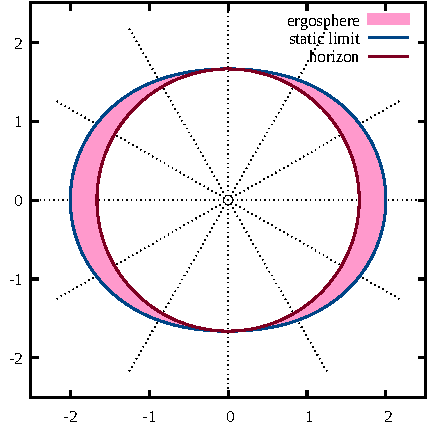
\includegraphics[width=0.7 \textwidth]{gfx/ergosphere.pdf}
	 \end{figure}
	 In the pink area between the two limits, one can in principle still escape from the black hole but can not be stationary against the outside world. The ergosphere is a region located outside a rotating black hole's outer event horizon. The ergosphere touches the event horizon at the poles of a rotating black hole and extends to a greater radius at the equator.  The equatorial (maximal) radius of an ergosphere corresponds to the Schwarzschild radius of a non-rotating black hole; the polar (minimal) radius can be as little as half the Schwarzschild radius (the radius of a non-rotating black hole) in the case that the black hole is rotating maximally (at higher rotation rates the black hole could not have formed). \\
	 \\
	 As a black hole rotates, it twists spacetime in the direction of the rotation at a speed that decreases with distance from the event horizon. This process is known as the Lense–Thirring effect or frame-dragging. By virtue of this dragging effect, an object within the ergosphere cannot appear stationary with respect to an outside observer at a great distance unless that object were to move at faster than the speed of light (an impossibility) with respect to the local spacetime. The speed necessary for such an object to appear stationary decreases at points further out from the event horizon, until at some distance the required speed is that of the speed of light. The set of all such points defines the ergosphere surface, called \emph{ergosurface}. The outer surface of the ergosphere is called the \emph{static surface or static limit}. This is because world lines change from being time-like outside the static limit to being space-like inside it. It is the speed of light that arbitrarily defines the ergosphere surface. Such a surface would appear as an oblate that is coincident with the event horizon at the pole of rotation, but at a greater distance from the event horizon at the equator. Outside this surface, space is still dragged, but at a lesser rate.
	 
	 \item Since the hypersurface $H$ is defined by the condition $∆ = 0$, its normal
	 vectors are given by
	 \begin{equation}
	 	\mathrm{grad} \Delta = \md \Delta^{\#}, \quad \md \Delta = 2(r-m) \md r.
	 \end{equation}
Thus, the norm of the normal vectors is 
\begin{equation}
 	\langle \mathrm{grad} \Delta, \mathrm{grad} \Delta \rangle = 4 g^{rr} (r-m)^2 \propto \Delta = 0
\end{equation}
on the hypersurface, showing that $H$ is a \emph{null hypersurface}. Because of this fact, the tangent space to
the null hypersurface $H$ at any of its points is orthogonal to a null vector,
and hence it does not contain time-like vectors, i.e. \textbf{you cannot cross the inner horizon $H$ ?}
\begin{mybox}{Killing horizon and ergosphere}
	The surface $H$ is called a \emph{Killing horizon}. The hypersurface defined
	by the static limit is time-like, which means that it can be crossed in
	both directions, in contrast to the horizon $H$. The region in between
	the static limit and the Killing horizon is the ergosphere, in which $k$ is
	space-like and no observer can be prevented from following the rotation
	of the black hole.
\end{mybox}
Associated to a Killing horizon is a geometrical quantity known as surface gravity, $\kappa$ . If the surface gravity vanishes, then the Killing horizon is said to be degenerate. The temperature of \emph{Hawking radiation} is related to the surface gravity $\kappa c^2$, $T_H=\frac {\hbar c\kappa }{2\pi k_{B}}$.
\item If you bend/twist spacetime too much, it breaks, gets holes and thus singularities are formed (c.f. singularity theorems by Penrose and Hawking \ref{sec:singularityHawkingPenrose}).
\item Formally, the Kerr solution is singular where $∆ = 0$, but this is a coordinate singularity.
\item Observer at static limit sends signal $\tilde{k}$ to static observer ($u=(t,\vec{0})^T$) far away:\\
	Observers at rest in a stationary space-time have four-velocities proportional to the Killing vector field $k$,
	\begin{equation}
		u \propto k, \quad u=\frac{k}{\sqrt{-\langle k,k\rangle}} = \frac{k}{\sqrt{-g_{tt}}}.
	\end{equation}
	We have seen that the projection of a Killing vector $K$ on a
	geodesic $γ$ is constant along that geodesic, $∇_{\dot{\gamma}}̇ \langle \dot{\gamma}, K\rangle = 0$. The light ray
	propagating from the source to the observer is a null geodesic with $\dot{\gamma}̇ = \tilde{k}$,
	hence
	\begin{equation}
		\nabla_{\tilde{k}} \langle \tilde{k},k\rangle =0
	\end{equation}
	and thus $\langle \tilde{k},k \rangle_0=\langle \tilde{k},k \rangle_s$. Using this we find
	\begin{align}
	1+z &= \frac{\nu_{src}}{\nu_{obs}} = \frac{\langle \tilde{k},u\rangle_{src}}{\langle \tilde{k},u\rangle_{obs}} \\
	&= \frac{\sqrt{-g_{tt}}_{obs} }{\sqrt{-g_{tt}}_{src}} \underbrace{\frac{\langle \tilde{k},k \rangle_{src}}{\langle \tilde{k},k \rangle_{obs}}}_{=1} .
	\end{align}
For an observer at rest far away from the black hole, $\langle \tilde{k},k\rangle_{obs} \approx- 1$, and the redshift becomes
\begin{equation}
	1+z \approx \frac{1}{\sqrt{-\langle \tilde{k},k\rangle_{src}}} =(- g_{tt})^{-\half}
\end{equation}
which tends to infinity as the source approaches the static limit, i.e. already at the outer horizon.\\
For a distant observer, $g_{tt} = \eta_{tt} = -1$. For the observer at static limit we further know that $\omega_- = 0 \Leftrightarrow g_{tt} \stackrel{!}{=}0$. Thus, $z\rightarrow \infty$ for source approaching the static limit. Static source here means swimming with the black hole drag. If you have proper acceleration, then $u \propto k$ is not satisfied anymore.
\item Einstein cat $\Rightarrow$ inside event horizon is region of spacetime causally disconnected from outside world; the discussed horizons are horizons \emph{against} the outside world. It is about defining the surface against whom. You are not dead as soon as $r<R_s$, you just can not communicate any more with the outside world.
\end{enumerate}
\subsubsection{Motion near a Kerr-Black Hole}
	Consider the motion of a non-charged object on a circular orbit in the equatorial plane around the black hole, i.e. $\dot{r}=0=q, \vartheta=\pi/2$.
	The Lagrangian becomes:
	\begin{equation}
		\mL = \half \left[- \left(1 - \frac{2m}{r} \right) \dot{t}^2 \underbrace{- \frac{4 m a}{r} \dot{t} \dot{\varphi}}_{=(g_{t\varphi}+g_{\varphi t}) \dot{x}^t \dot{x}^{\varphi}} + (r^2+a^2+2ma^2) \dot{\varphi}^2\right].
	\end{equation}
	Since $\dot{r}$ is a cyclic coordinate, the Euler-Lagrange equations yield a force equation which tell us where we an have a stable radial orbit:
	\begin{equation}
		\underbrace{\frac{\partial \mL}{\partial r}}_{"\frac{\partial F}{\partial r}"=0} = \frac{\md}{\md t} \frac{\partial \mL}{\partial \dot{r}}=0 ;\Rightarrow\;\frac{\partial \mL}{\partial r} = 0.
	\end{equation}
 This is equivalent to the following.
 \begin{mybox}{Kepler's third law for the KN-black hole}
 	For $\omega=\frac{\md \varphi}{\md t} = \frac{\dot{\varphi}}{\dot{t}}$ one finds two solutions of the radial equation
 	\begin{equation}
 		\omega_{\pm} = \pm \sqrt{m} \frac{1}{r^{\frac{3}{2}} \pm \sqrt{m}a}.
 	\end{equation}
 	The sign tells us that the frequency depends on whether the test particle moves with or against the rotation (i.e. with or against the induced frame drag of spacetime) of the black hole.
 \end{mybox}
Trajectories of test particles in the vicinity of a Kerr black hole look like the following figure \ref{fig:trajectorieskerrbh}.
\begin{figure}
	\centering
	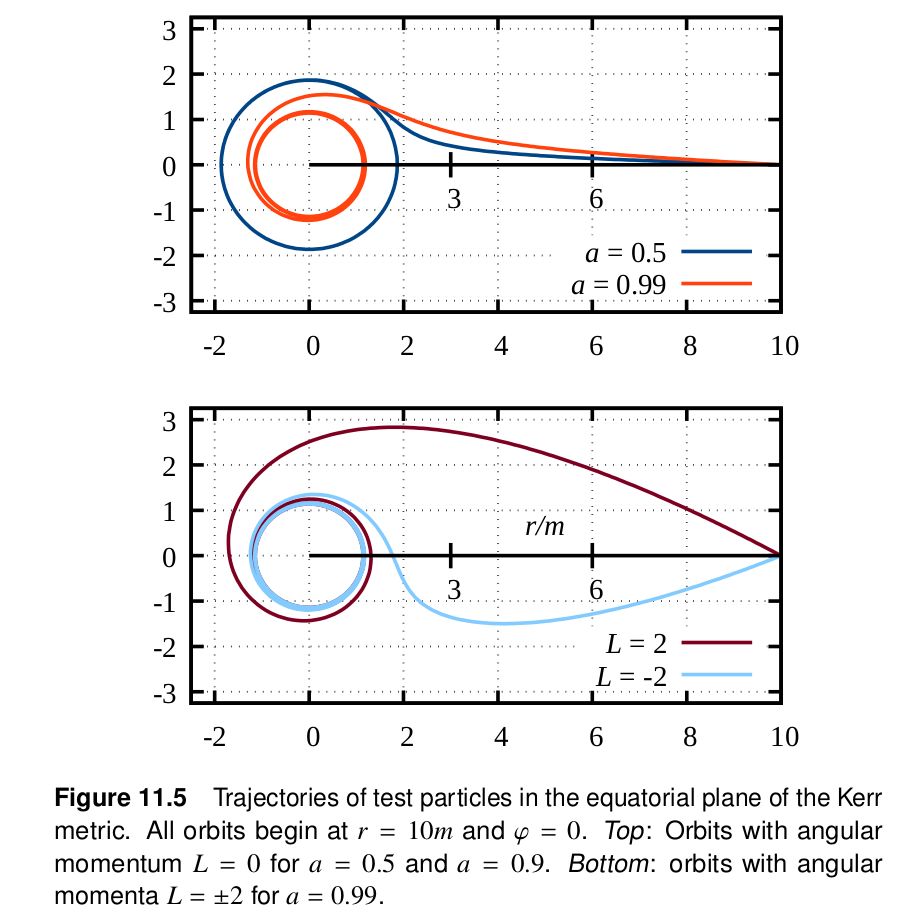
\includegraphics[width=0.7\textwidth]{gfx/TrajectoriesKerrBH}
	\caption{}
	\label{fig:trajectorieskerrbh}
\end{figure}
	
	
	\newpage
	
	\subsection{Entropy and Temperature of a Black Hole}
	Is there a violation of the second law of thermodynamics taking place by a black hole taking in object with entropy, but not giving anything back, i.e does the entropy of the Universe decrease by this ? $\rightarrow$ Assign an entropy to the BH itself.\\
	It was realised by Stephen Hawking, Roger Penrose and Demetrios
	Christodoulou that the area of a possibly charged and rotating black hole,
	defined by
	\begin{equation}
		A = 4 \pi \alpha := 4 \pi (r^2_+ + a^2), \quad r_{\pm} = m \pm \sqrt{m^2-Q^2-a^2},\, \vec{a}=\frac{\vec{L}}{M c} = \frac{\mathcal{G} \vec{L}}{c^3 m},
	\end{equation}
	cannot shrink $\Rightarrow A \equiv S ?$.\\
	\\
	This led Jacob Bekenstein (1973) to the following consideration. If $A$
	cannot shrink, it reminds of the entropy as the only other quantity known
	in physics that cannot shrink. Could the area $A$ have anything to do
	with an entropy that could be assigned to a black hole? In fact, this is
	much more plausible than it may appear at first sight. Suppose radiation
	disappears in a black hole. Without accounting for a possible entropy of
	the black hole, its entropy would be gone, violating the second law of
	thermodynamics. The same holds for gas accreted by the black hole: Its
	entropy would be removed from the outside world, leaving the entropy
	there lower than before.\\
	\\
	If, however, the increased mass of the black hole led to a suitably in-
	creased entropy of the black hole itself, this violation of the second law
	could be remedied.
	\begin{mybox}{Analogy between area and entropy}
	Any mass and angular momentum swallowed by a black hole leads to
	an increase of the area $A$, which makes it appear plausible that
	the area of a black hole might be related to its entropy
	\end{mybox}
	Try to derive an analogue to the first law of thermodynamics:\\
	Calculate all the derivatives appearing in
	 \begin{equation}
	 	\md \alpha = 2 (r_+ \md r_+ + \vec{a} \cdot \md \vec{a}), \quad \delta r:= r_+ - r_,
	 \end{equation}
	 to find
	 \begin{equation}
	 	\md m =\underbrace{ \frac{\delta r}{4 \alpha } \md \alpha}_{ \Theta\md S} +\underbrace{ \frac{r_+}{\alpha} Q \md Q + \frac{\mathcal{G}}{c^3} \frac{\vec{a}\cdot \md \vec{L}}{\alpha }}_{"Work"}
	 \end{equation}
	 where the work is work exerted on the black hole from outside world (change $\vec{L}, Q$...). This reminds of the first law of thermodynamics if we tentatively associate $m$ with the internal energy, $α$ with the entropy and the remaining
	 terms with external work. \\
	 \\
	 \marginpar{Planck units: $\lambda_{pl} = \frac{\hbar}{M_{pl} c}$ planckian compton wavelength, then the gravitational binding energy has to stabilize rest energy: $\frac{\mathcal{G}M^2_{pl}}{\lambda_{pl}} \stackrel{!}{=} M_{pl} c^2$, thus $M^2_{pl} = \frac{\hbar c}{\mathcal{G}}$, $\lambda^2_{pl} = \frac{\mathcal{G} \hbar}{c^3}$. Further, $E_{pl} = M_{pl} c^2$, i.e. $T_{pl} = \frac{E_{pl}}{k_B}$.}
	 Let us now see whether a linear relation between the entropy $S$ and the
	 area $α$ will lead to consistent results. Thus, assume $S = γα$ with some
	 constant $γ$ to be determined. Then, a change $δα$ will lead to a change
	 $δS = γδα$ in the entropy. Bekenstein showed that the minimal change of the effective area is twice
	 the squared Planck length, thus
	 \begin{equation}
	 	\delta \alpha =2 \frac{\mathcal{G}\hbar}{c^3}.
	 \end{equation}
	 On the other hand, he identified the minimal entropy change of the black
	 hole with the minimal change of the Shannon entropy, which is derived
	 from information theory and is
	 \begin{equation}
	 	S = k_B \ln 2,
	 \end{equation}
	 where the Boltzmann constant $k_B$ was inserted to arrive at conventional
	 units for the entropy. This could e.g. correspond to the minimal information loss when a single particle disappears in a black hole.
	\begin{mybox}{Bekenstein entropy }
		The Bekenstein entropy of a black hole is
		\begin{equation}
			S = \frac{\ln 2}{8  \pi } k_B \frac{c^3}{\mathcal{G} \hbar} A,
		\end{equation}
		where $A$ is the area of the black hole. This assignment was motivated by trying to save the thermodynamic laws, don't know if it is true.
	\end{mybox}
	With $E=Mc^2= \frac{m c^4}{\mathcal{G}}$, we find 
	\begin{equation}
		\frac{1}{T} = \left(\frac{\partial S}{\partial E}\right)_{V,N} = \frac{\ln 2}{2} k_B \underbrace{\left(\frac{\partial \alpha}{\partial m}\right)_{Q,L}}_{\frac{1}{\Theta}},= \ln 2 \frac{k_B \mathcal{G} M}{\hbar c^3}.
	\end{equation}
\begin{mybox}{Temperature of a Black Hole}
The analogy between the area of a black hole and entropy implies that
black holes can be assigned the temperature
\begin{equation}
	T = \frac{2}{\ln 2} \frac{\hbar c}{k_B} \Theta= \frac{2 \pi}{\ln 2} \frac{\hbar c}{k_b} \frac{\delta r}{A} = \frac{T_{pl}}{\ln 2} \left(\frac{M_{pl}}{M}\right),
\end{equation}
where the latter equality holds for an uncharged and non-rotating black hole.
\end{mybox}
	
	This result leads to a remarkable conclusions:
	\begin{enumerate}
		\item  If black holes have a
	temperature, they will radiate and thus lose energy or its mass equivalent. They can therefore evaporate.
	
	\item As the mass increases, temperature goes down. This system defies the 3rd law of thermodynamics ($S=0$ at $T=0$, since
	\begin{equation}
		T \propto \frac{1}{M}.
	\end{equation}
	Since $T ∝ M^{−1}$ and $S ∝ M^2$ , where $M$ is the black-hole mass, one has $S → ∞$ for $T → 0$, in
	gross contrast to the statement from classical thermodynamics.\\
	But there is some fundamental analogy between BH(areas) and thermodynamics.
	\item If bh has $T>0$ finite temperature, it has to radiate, it has a luminosity, this is  \emph{Hawking radiation}.\\
	The black hole thus must evaporate. The evaporation time is the slower the lower its mass.\\
	Note that $\alpha$ only does \emph{not descrease} if you neglect the loss by Hawking radiation (think of microcanonical ensemble without exterior particle exchange ??).
	
	\item $T$ is equivalent to the temperature of (Planck) spectrum of a(n) (anti-)particle whose partner anti(particle) has fallen into the bh. This can be computed by solving the corresponding QFT on a curved spacetime in the vicinity of the black hole.
	\item $S=\gamma \alpha$ is identification of the interior of bh (of which we do not and can not have any knowledge due to horizon) with the exterior world. Thus, identify processes interior with $\alpha$, which implies the use of the\emph{holographic principle} (map interior onto surface of bh), c.f. \emph{AdS/CFT correspondence}..
	 \item For a black hole of solar mass, the temperature is $T=5\times 10^{-7} \mathrm{K}$.
	 \item This analogy for $S_{BH}$ is additive w.r.t the are of the black hole, and not w.r.t the mass, since they are inverse proportional, but it has to be this way since GR is not linear, you can not superpose the gravitational effect of different masses.
\end{enumerate}
	
	
	
	
	
\section{Cosmology}
Cosmology is one of the biggest application of GR. We will therefore treat it in a separate chapter.

\chapter{Cosmology}

\section{Homogeneous and Isotropic Cosmology - GR perspective}
\subsection{Spherically-symmetric space-times}
Physical cosmology aims at studying the structure and evolution of the
universe as a whole. Of the four fundamental interactions of physics,
only gravity is relevant on the largest scales because the strong and
the weak interactions are confined to sub-atomic length scales, and the
electromagnetic force is shielded on large scales by opposite charges.
We thus expect that the space-time of the Universe can be idealised as
a solution of Einstein’s field equations, satisfying certain simplicity requirements expressed by symmetries imposed on the form of the solution.
In this chapter, we shall therefore first discuss spherically-symmetric
space-times in general and then specialise them to cosmological solutions
in particular.

\subsubsection{Form of the metric}
Generally, a space-time (M, g) is called \emph{spherically symmetric} if it admits
the group $SO(3)$ as an isometry such that the group’s orbits are two-
dimensional, space-like surfaces. Space-like hypersurface means that all normal vectors of these hypersurfaces are time-like, or that the corresponding tangent vectors are space-like.
For any point $p \in M$, we can then select the orbit $Ω(p)$ of $SO(3)$ through
$p$. In other words, we construct the spatial two-sphere containing $p$
which is compatible with the spherical symmetry. I.e. take $p\in M$, construct orbit around $p\Rightarrow$ get a sphere. This is the group orbit of $\Omega(p)$. On this sphere use coordinates $(\vartheta, \varphi)$.

\begin{figure}[h!]
	\centering
	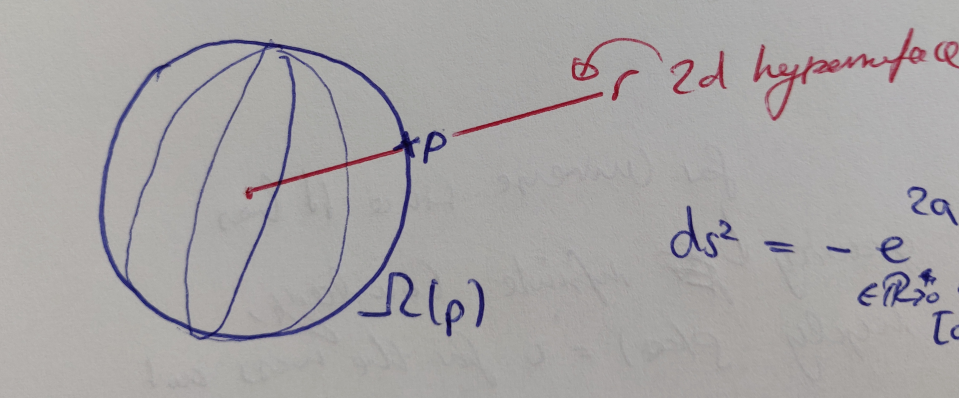
\includegraphics[width=0.7\linewidth]{gfx/SphericallySymmetricSpacetime}
	\caption{\itshape Group orbits around point make up $S^2$, the orthogonal space is $N(p)$.}
	\label{fig:sphericallysymmetricspacetime}
\end{figure}

Next, we construct the set of all geodesics $N(p)$ through $p$ which are
orthogonal to $Ω(p)$. Locally, $N(p)$ forms a two-dimensional surface
which we also call $N(p)$. Repeating this construction for all $p \in M$
yields the surfaces $N$.
We can now introduce coordinates $(r, t)$ on $N$ and $(θ, φ)$ on $Ω$, i.e. such
that the group orbits $Ω$ of $SO(3)$ are given by $(r, t) = const.$ and the
surfaces $N$ by $(θ, φ) = const.$ With these adapted coordinates, the metric has the following line element.
\begin{mybox}{Metric of a spherically-symmetric space-time}
	The line element of the metric of a spherically-symmetric space-time
	M can be written in the form
	\begin{equation}
	\md s^2 = \md \tilde{s}^2 + R(t,r) \md \Omega^2
	\end{equation}
	where $\md \tilde{s}^2$ is the line element of a yet unspecified metric $\tilde{g}$ in the
	coordinates $(t, r)$ on the surfaces $N$. This is equivalently derived from the theory of maximally symmetric spaces in \ref{eq:metricsphericallysymmetricspacetime}
	Without loss of generality, we can now choose $t$ and $r$ such that the
	metric $\tilde{g}$ is diagonal, which allows us to write its line element as
	\begin{equation}
	\md \tilde{s}^2 = -e^{2a(t,r)} \md t^2 +e^{2 b(t,r)} \md r^2
	\end{equation}
	with functions $a(t, r)$ and $b(t, r)$ to be determined, now time-dependent !
\end{mybox}
The chosen dual basis then is
\begin{equation}
\theta^0 = e^a \md t, \, \theta^1 =e^b \md r, \; \theta^2 = R \md \vartheta, \; \theta^3 = R \sin \vartheta \md \varphi.
\end{equation}


\subsubsection{Generalised Birkhoff's theorem}
\begin{mybox}{Birkhoff's generalized theorem}
	Every $C^2$ solution of Einstein’s vacuum equations which is spherically
	symmetric in an open subset $U \subset M$ is locally isometric to a domain
	of the Schwarzschild-Kruskal solution.
\end{mybox}
Now we don't want a static or stationary solution, we don't have a preffered time direction. 
\begin{mybox}{Cavity in spherically-symmetric space-time}
	It is a corollary to Birkhoff’s theorem that a spherical cavity in a
	spherically-symmetric spacetime has the Minkowski metric. Indeed,
	Birkhoff’s theorem says that the cavity must have a Schwarzschild
	metric with mass zero, which is the Minkowski metric.
\end{mybox}


\subsection{Homogeneous and Isotropic Space-times}
There are good reasons to believe that the Universe at large is \emph{isotropic}
around our position. The most convincing observational data are provided by the cosmic microwave background, which is a sea of black body
radiation at a temperature of $(2.725 ± 0.001) K$ whose intensity is almost
exactly independent of the direction into which it is observed.\\
\\
There is furthermore no good reason to believe that our position in the
Universe is in any sense preferred compared to others.  This is known as the \emph{Cosmological Principle}: all positions in the universe are essentially equivalent. The Cosmological Principle can be formulated as a statement about the existence of equivalent coordinate systems. A different set of space-time coordinates $x^{\prime \mu}$ must be \emph{equivalent} to some fiducial cosmic standard coordinates $x^\mu$ (the fiducial coordinate frame of the CMB), if the whole history oft he universe appears the same in the $x^{\prime \mu}$ as in the fiducial coordinate system $x^\mu$ This simply says that the coordinate transformation $x^\mu\rightarrow x^{\prime\mu}$ must be an \emph{isometry} and than the tensors $g\munu, T\munu$ must be \emph{form-invariant} under this transformation. We must therefore
conclude that any observer sees the cosmic microwave background as an isotropic source such as we do. Then, the Universe must also be
\emph{homogeneous}.\\
\\
We are thus led to the expectation that our Universe at large may be
described by a homogeneous and isotropic space-time. Let us now give
these terms a precise mathematical meaning.
\begin{mybox}{Spatially homogeneous space-time}
	A space-time $(M, g)$ is called \emph{spatially homogeneous} if there exists a
	one-parameter family of space-like hypersurfaces $\Sigma_t$ that foliate the
	space-time such that for each $t$ and any two points $p, q ∈ \Sigma_t$ , there exists
	an isometry $φ$ of $g$ which takes $p$ into $q$.\\
	$"g(q) = g(q+p)"$.
\end{mybox}
\begin{figure}[h!]
	\centering
	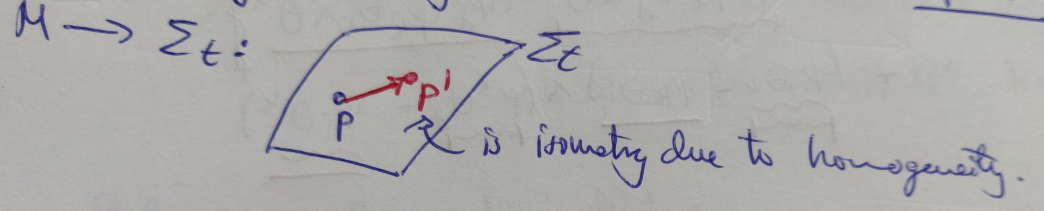
\includegraphics[width=0.7\linewidth]{gfx/HomogeneousSpacetime}
	\caption{\itshape The isometry is a translation relating points on the space-like hypersurface.}
	\label{fig:homogeneousspacetime}
\end{figure}




Before we can define isotropy, we have to note that isotropy requires that
the state of motion of the observer needs to be specified first because two
observers moving with different velocities through a given point in space-
time will generally observe different redshifts in different directions. Spatial isotropy is thus observer dependent.
\begin{mybox}{Spatially isotropic space-time}
	Therefore, we define a space-time $(M, g)$ as spatially isotropic about a
	point $p$ if there exists a congruence of time-like geodesics through $p$
	with tangents $u$ such that for any two vectors $v_1 , v_2 \in T_p M$ orthogonal
	to $u$, there exists an isometry of $g$ taking $v_1$ into $v_2$ but leaving $u$ and
	$p$ invariant. In other words, if the space-time is spatially isotropic, no
	preferred spatial direction orthogonal to $u$ can be identified.\\
	\\Caroll:More formally, a manifold $M$ is isotropic around a point $p$ if, for any two vectors $V$ and $W$
	in $T_p M$, there is an isometry of $M$ such that the pushforward of $W$ under the isometry is
	parallel with $V$ (not pushed forward).
\end{mybox}
\begin{figure}
	\centering
	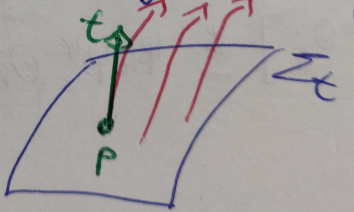
\includegraphics[width=0.7\linewidth]{gfx/IsotropicSpacetime}
	\caption{\itshape The space-time is isotropic w.r.t. the preferred flow defining a bundle of time-like geodesics which are related by isometries.}
	\label{fig:isotropicspacetime}
\end{figure}


Isotropy thus identifies a special class of observers, with four-velocities
$u$, who cannot identify a preferred spatial direction. The spatial hypersurfaces $\Sigma_t$ must then be orthogonal to $u$ because otherwise a preferred
direction could be identified through the misalignment of the normal
direction to $\Sigma_t$ and $u$, breaking isotropy.\\
All coordinates systems that are equivalent to the fiducial cosmic standard system necessarily use cosmic standard time. The assumption of spatial isotropy can therefore equivalently following Weinberg be formulated as the requirement that there exists a family of coordinate systems $x^{\prime \mu}(x;\theta)$, depending on the three independent parameters $\theta^1,\theta^2,\theta^3$, which are equivalent to the cosmic standard coordinates, and which have the same origin, that is,
\begin{equation}
x^{\prime i}(0,t;\theta)=0
\end{equation}
We can intuitively think of the three parameters $\theta^n$ as Euler angles that specify the orientation of the $x^{\prime i}$ coordinate axes relative to the $x^i$ coordinate axes of the fiducial system; the important thing is that there be \emph{three} independent parameters. (In formulating this assumption, we have \textbf{tacitly assumed that the privileged Lorentz frame in which the universe appears isotropic happens to coincide more or less with the origin of the fiducial coordinate system, which is the CMB}.)
\\
Formulating the assumption of homogeneity: Clearly, homogeneity does not mean that any object can be chosen as the origin of a coordinate system equivalent to our cosmic standard coordinates -  after all, the universe looks different to an observer moving away from the Liky Way at half the speed of light than it does to us. The most we can expect is that every point $x^\mu$ in space-time is on some "fundamental  trajectory" $x^i=X^i(t)$ (Hubble flow), which can serve as the origin of a coordinate system $x^{\prime \mu}$ equivalent to the cosmic standard system. The important point is that, since the $\vec{X}(t)$ at any time $t$ fill up all space, they are determined by \emph{three} independent parameters $a^i$. Thus homogeneity means that there is a three-parameter set of cordinates $\bar{x}^{\prime \mu}(x;a)$, which are equivalent to the cosmic standard coordinates $x^\mu$, and which have origin on the trajectory $x^i=X^i(t;a)$, that is,
\begin{equation}
\bar{x}^{\prime i}(\vec{X}(t;a),t;a) =0.
\end{equation}
To be more precise, the $\vec{X}(t;a)$ are \emph{the trajectories of the privileged observers to whom the universe appears isotropic}, i.e. \emph{observers comoving with the Hubble flow.}
\\
We thus arrive at the following conclusions: a homogeneous and isotropic
space-time $(M, g)$ is foliated into space-like hypersurfaces $\Sigma_t$ on which $g$
induces a metric $h$. There must be isometries of $h$ carrying any point $p \in \Sigma_t$ into any other point $q \in \sigma_t$ . Because of isotropy, it must furthermore	be impossible to identify preferred spatial directions on $\Sigma_t$ . These are
very restrictive requirements which we shall now exploit.
\subsubsection{Assumptions imply Killing vectors}
Putting the above together, we see that the Cosmological Principle entails the existence of two independent three-parameter families of coordinate transformation $x\rightarrow x^\prime$, $x\rightarrow\bar{x}^\prime$, which are isometries and which leave the time coordinate invariant. Descend to the case of infinitesimal transformations, letting $a^i, \theta^i$ approach zero, lets us find six "Killing vectors" $\xi^\mu_j(x)$ and $\bar{\xi}^\mu_j(x)$, defined by
\begin{align}
	\label{eq:cosmologicalKillingVectors}
	\xi^i_j(x) & \equiv \frac{\partial x^{\prime i}(x;\theta)}{\partial \theta^j} |_{\vec{\theta}=0} \qquad  \xi^t_j(x)\equiv=0\\
	\bar{\xi}^i_j(x) &\equiv \frac{\partial \bar{x}^{\prime i} (x;a)}{\partial a^j} |_{\vec{a}=0} \qquad \bar{\xi}^i_j(x)\equiv 0.
\end{align}
Thus we have six independent Killing vectors with $\xi^t=0$, the maximum number possible in three dimensions. The universe therefore satisfies the requirements for a four-dimensional space with three-dimensional maximally symmetric subspaces $\Sigma_t$ with $t=$constant.\\
The cosmological Principle can therefore be formulated in the language of Maximally symmetric spaces as follows:
\begin{enumerate}
	\item The hypersurfaces with constant cosmic standard time are maximally symmetric subspaces of the whole space-time.
	\item Not only the metric $g\munu$, but all cosmic tensors such as $T\munu$ are form-invariant w.r.t. the isometries of these subspaces.
\end{enumerate}





\subsubsection{Line of Reasoning - Weinberg}
The Cosmological Principle allows the specification of the cosmic metric entirely in terms of a "radius" $R(t)$ and a trichotomic constant $k$, as in \ref{eq:metricRobertsonWalkerViaMaximalSymmetry}, and we shall then see how astronomical observations can be interpreted as measurement of $R(t)$ and $k$.\\
This inherently kinematic approach, pioneered in the 1930's by Robertson and Walker, is incomplete in that it does not provide and \emph{a priori} prediction of the function $R(t)$. To calculate $R(t)$ we need to make some assumption about the material content of the universe, and then derive the Robertson-Walker metric as a solution of the Einstein field equations \ref{eq:metricRobertsonWalkerViaField}, as first done by Friedmann in 1922.\\
\\
Weinberg makes the distinction to call this section cosmography and later discussion on the contents of the universe cosmology, why this distinction between cosmography and cosmology ? The reason is simply that we do not know the equation of state of the matter and radiation of the universe throughout its history, and even if we did, we could not be sure that the Einstein equations really hold over cosmic times and distances. A modification of the field equations or the equations of state, such as the introduction of a cosmological constant, or a large population of gravitons, \emph{would affect $R(t)$ and invalidate the simplest Friedmann solution, but it wuld not require us to make any change in the descriptive framework assembled in this chapter}.\\
\emph{If the data of observations will not fit into this framework, we shall be able to conclude that either the Cosmological Principle or the Principle of Equivalence is wrong. Nothing could be more interesting.}








\subsubsection{Spaces of constant curvature}
Consider now the curvature tensor $^{(3)}\bar{R}$ induced on $\Sigma_t$  (i.e. the curvature
tensor belonging to the metric $h$ induced on $\Sigma_t$ ):
\begin{equation}
^{(3)} \bar{R} = ^{(3)}\bar{R}^{\;\, kl}_{ij}.
\end{equation}
In this way, $^{(3)} \bar{R}$ represents a linear map from the vector space of 2-forms $\bigwedge^2$into $\bigwedge^2$ , because of the antisymmetry of $^{(3)}\bar{R}$ with respect to
permutations of the first and the second pairs of indices. Thus, it defines
an endomorphism:
\begin{equation}
L:\bigwedge^{\,2} \rightarrow \bigwedge^{\,2}, \quad ^{(3)} \bar{R}^{\,\,kl}_{ij} \omega_{kl} = (L\omega)_{ij} \, \in \bigwedge^2.
\end{equation}
Due to the symmetry of $^{(3)}\bar{R}$ upon swapping the first with the
second pair of indices, the endomorphism $L$ is self-adjoint. In fact, for any pair of 2-forms $α, β \in \bigwedge^2: \langle \alpha, L \beta \rangle = \langle \beta, L \alpha>$. Every self-adjoint endomorphism defines an orthonormal set of eigenvectors (3 of them), which have all the same eigenvalue by isotropy assumption:
\begin{equation}
L = id \cdot 2 k
\end{equation}
where $k$ is the \emph{spatial curvature parameter}.
Then, by this endomorphism the induced spatial curvature still has to be antisymmetric in both index pairs:
\begin{equation}
^{(3)}\bar{R}_{ij}^{kl} = k \left[\delta^k_i \delta^l_j - \delta^k_j \delta^l_i \right]\, \Rightarrow \, ^{(3)}\bar{R}_{ijkl} = k \left[h_{ik} h_{jl} - h_{jk} h_{il}\right],
\end{equation}
where the indices where lowered by means of the induced metric $h$. Then
\begin{equation}
^{(3)}R_{jl} = 2 k h_{jl} \quad \Rightarrow \quad ^{(3)} \mathcal{R}= 6 k.
\end{equation}
The curvature forms are then found to be
\begin{equation}
\Omega^i_j = \frac{1}{2} ^{(3)} \bar{R}^i_{jkl} \theta^k \wedge \theta^l = k \theta^i \wedge \theta_j.
\end{equation}

The curvature parameter k must be (spatially) constant because of homogeneity.
\begin{statements}
	Space-times with constant curvature can be shown to be
	conformally flat.
\end{statements}
This means that coordinates can be introduced in
which the line element $dl^2$ of the metric $h$ reads
\begin{equation}
\md l^2 = \frac{1}{\psi^2} \sum_{i=1}^{3} (\md x^i)^2.
\end{equation}
The modus operandi is now to fix the conformal factor $\psi$ such that $\md l^2$ and $\Omega^i_j$ agree: \\
Start as always by introducing cotetrad to have a Euclidean metric.  The isotropy of our coordinates implies that
\begin{equation}
\psi = \sum_{k=1}^{3} f_k(x^k).
\end{equation}
Catan's structure equations then yield an equation for $\psi$ and $f_k$ such that one finds with $\sum_{i=1}^{3} (x^i)^2=r^2$ and with a specific choice of coordinates
\begin{equation}
\md l^2 = \frac{\sum_i (\md x^i)^2}{\left[1+\frac{k}{4} r^2\right]^2}
\end{equation}
\todo{ Include derivation of curvature forms, how you identify the $k$ and then derive geometric tensors.}
\subsection{Friedmann's equations}
\subsubsection{Connection and curvature forms}
This yields the metric of the four-dimensional space-time. Use the order parameter $t=const.$ of our spatial hypersurfaces $\Sigma_t$ as our time coordinate and choose coordinates such that $g_{00}=1$ and $g_{0i}=0$. Metric doesn't have to look like that, but we choose it such that the former conditions are satisfied.	
\begin{mybox}{Robertson-Walker metric}
	According to the preceding discussion, the homogeneous and isotropic
	spatial hypersurfaces $\Sigma_t$ must have a metric $h$ with a line element of the
	form
	\begin{equation}
	\md l^2 = \frac{\sum_{i=1}^{3}(x^i)^2}{\left(1+\frac{r^2k}{4}\right)^2}, \quad r^2 \equiv \sum_{i=1}^{3} (x^i)^2.
	\end{equation}
	By a suitable choice of the time coordinate $t$, the line element of the
	metric of a spatially homogeneous and isotropic space-time can then
	be written as
	\begin{equation}
	\label{eq:metricRobertsonWalkerViaField}
	\md s^2 = -c^2 \md t^2 + a^2(t) \md l^2
	\end{equation}
	because the scaling function $a(t)$ must not depend on the $x^i$ in order to
	preserve isotropy and homogeneity. This metric  of a spatially
	homogeneous and isotropic space-time is called \emph{Robertson-Walker}
	metric.
\end{mybox}
\begin{mybox}{Alternative forms of the metric}
	We thus find that the homogeneous and isotropic class of cosmological
	models based on Einstein’s field equations are characterised by the line
	element
	\begin{equation}
	\md s^2 = -c^2 \md t^2 + a^2(t) \left[\md \omega^2 + f^2_k(\omega) \left(\md \vartheta^2 + \sin^2 \vartheta \md \varphi^2\right)\right]
	\end{equation}
	with 
	\begin{equation}
	f_k(\omega)=\left\{	\begin{array}{lr}
	{k}^{- \half} \sin(k^{\half} \omega) & \mathrm{if} \, k>0\\
	\omega 												& 			\mathrm{ if} \, k=0 \\
	\abs{k}^{- \half} \sinh( \abs{k}^{ \half} \omega) & \mathrm{if} \, k<0.
	\end{array}			\right\}
	\end{equation}
	which is equivalent to
	\begin{equation}
	\md s^2 = -c^2\md t^2 + a^2(t) \left[ \frac{\md u^2}{1 - k u^2} +u^2\left( \md \vartheta^2 + \sin^2\vartheta \md \varphi^2 \right)\right]
	\end{equation}
	with $u$ related to $\omega$ by $u=f_k(\omega)$, and the scale factor $a(t)$ satisfies the
	Friedmann equations.
\end{mybox}
In a suitable tetrad, we find the geometric tensor quantities by Cartan's structure equations:
\begin{mybox}{Einstein tensor for a spatially homogeneous and isotropic
		space-time}
	The Einstein tensor of a spatially homogeneous and isotropic space-
	time has the components
	\begin{align}
		G_{00}&= 3\frac{k+\dot{a}^2/c^2}{a^2}, \quad G_{11}=G_{22}=G_{33} =-\frac{2 \ddot{a}}{a c^2}- \frac{k+\dot{a}^2/c^2}{a^2} \\
		\mathcal{R} &= 6 \left(\frac{\ddot{a}}{a c^2} + \frac{k+\dot{a}^2/c^2}{a^2}\right)\\
		R_{00}& =- \frac{3 \ddot{a}}{a c^2}, \; R_{11}=R_{22}=R_{33}=\frac{\ddot{a}}{a c^2} + 2\frac{k+\dot{a}^2/c^2}{a^2}.
	\end{align}
\end{mybox}
\subsubsection{On the Robertson-Walker metric - Weinberg}
As for the treatment of maximally symmetric subspaces, we see that the cosmological symmetries allows us to arrive at the Robertson-Walker metric \ref{eq:metricRobertsonWalkerViaMaximalSymmetry}, where the time coordinate appearing $t$ is the standard cosmic time, but could also be a function of it.\\
Note that for $k=-1$ or $k=0$ the space is infinite, while for $k=+1$ it is finite (though unbounded).\\
For $k=+1$ the spatial universe can be regarded as the surface of a sphere of radius $R(t)$ in four-dimensional Euclidean space, and $R(t)$ can justly be called the "radius of the universe". $R(t)$ sets the scale of the geometry of the space, so $R(t)$ will in all cases be called the \emph{cosmic scale factor}, i.e. $R(t)\equiv a(t)$.
\\
\\
Fixing the trajectories of comoving observers by attaching them to the Hubble flow, we can conclude that the spatial coordinates $r,\theta,\phi$ form a \emph{comoving system}, in the sense that \emph{typical galaxies have constant spatial coordinates} $r,\theta,\phi$. One can imagine the comoving coordinate mesh to be like lines painted on the surface of a balloon, on which dots represent typical galaxies. As the balloon is inflated or deflated the dots will move, but the lines will move with them, so each dot will keep the same coordinates.\\
\\
It is important to note that the fundamental (comoving) trajectories $\vec{x}=$constant are geodesics, because \ref{eq:metricRobertsonWalkerViaMaximalSymmetry} gives
\begin{equation}
\Gamma^\mu_{tt} = 0.
\end{equation}
Thus the statement that a galaxy has constant $r,\theta,\phi$ is perfectly consistent with the supposition that galaxies are in free fall. Note also that the time coordinate $t$ in \ref{eq:metricRobertsonWalkerViaMaximalSymmetry} is not only a possible "cosmic standard" time; it is also the proper time told by a clock at rest in any typical freely falling galaxy. The coordinates $x,t$ are thus co-moving in precisely the same sense as the Riemannian normal coordinates.\\
The four-velocity of such a freely-falling or comoving observer is
\begin{equation}
U^t\equiv 1, \qquad U^i \equiv 0.
\end{equation}
This shows that \emph{the contents of the universe are, on the average, at rest in the coordinate system} $r,\theta,\phi$. Furthermore, one can from the comoving observer deduce that \emph{the energy-momentum tensor of the universe necessarily takes the same form as for a perfect fluid.}





\subsubsection{From Einstein to Friedmann}
For Einstein’s field equations to be satisfied, the energy-momentum
tensor must be diagonal, and its components must not depend on the
spatial coordinates in order to preserve isotropy and homogeneity. Spatial isotropy implies a preferred velocity field, together with spatial homogeneity one has one possible choice to built a rank $(0,2)$ tensor we need  by this preferred field: $u^{\flat} \otimes u^{\flat}$, the other symmetric $(0,2)$ tensor is $g$. Every other rank $(0,2)$ would have own set of eigenvectors, thus it would define a preferred direction in conflict with isotropy. We
set $T_{00} = ρc^2$ , which is the total energy density, and $T_{ij} = p δ_{i j}$ , where $p$
is the pressure.
This corresponds to the energy-momentum tensor of an ideal fluid,
\begin{equation}
T = (\rho c^2 + p) u^{\flat} \otimes u^{\flat}\quad + p g.
\end{equation}
In our adapted coordinates, $u^{\flat} = \md t$ and $g$ is Minkowskian. As seen by a fundamental observer (i.e. an observer for whom the spatial
hypersurfaces are isotropic). For such an observer, $u = \partial_t$ , and since the
metric is Minkowskian in the suitable tetrad we find
\begin{equation}
T = (\rho c^2+p) \md t\otimes \md t+ pg, \quad \left\{	\begin{array}{lr}
T_{00} = T(\partial_t,\partial_t) = \rho c^2 \\
T_{11} = p = T_{22} = T_{33},
\end{array}		\right\}
\end{equation}
where $\rho,p = \rho(t), p(t)$ only by isotropy. Equivalently, 
\begin{equation}
u^\mu= \partial_t=(1,0,0,0) \; \Rightarrow \quad T\munu=\begin{pmatrix}
\rho c^2 &0&0&\\
&&&&\\
&&g_{ij} p&&\\
&&&&
\end{pmatrix}.
\end{equation}
Which has the forms
\begin{equation}
T^\mu_\nu = \mathrm{diag}\left(-\rho c^2,p,p,p\right),\quad T= \tr T = -\rho c^2+ 3p.
\end{equation}
Does it follow from here that for $\tr T=0=-\rho c^2+3p$ $\Leftrightarrow p=\frac{\rho c^2}{3}$ for ultra-relativistic matter ? Answer: Radiation and ultra-relativistic matter both are called radiation and they both describe a perfect fluid. hence the adhere to this energy-momentum tensor. At the same time, radiation adheres to the energy-momentum tensor of em. field, whose trace vanishes. Thus, equation both energy momentum tensor and tracing both sides yields the ultra-rel. e.o.s.

This can be put into the Einstein field equations to find Friedmann equations by rearranging them.
\begin{mybox}{Friedmann's equations}
	For a spatially homogeneous and isotropic space-time with the
	Robertson-Walker metric, Einstein’s field equations reduce
	to Friedmann’s equations,
	\begin{align}
		\left(\frac{\dot{a}}{a}\right)^2 &=\frac{8 \pi \mathcal{G}}{3} \rho + \frac{\Lambda c^2}{3}- \frac{k c^2}{a^2}, \\
		\frac{\ddot{a}}{a} &= - \frac{4 \pi \mathcal{G}}{3} \left(\rho + \frac{3 p}{c^2}\right) + \frac{\Lambda c^2}{3}.
	\end{align}
	A Robertson-Walker metric whose scale factor satisfies Friedmann’s
	equations is called \emph{Friedmann-Lemaître-Robertson-Walker metric}.
	
\end{mybox}

\begin{mybox}{First law of thermodynamics}
	Combining both Friedmann equations yields the "first law of thermodynamics" in Cosmology
	\begin{equation}
	\frac{\md}{\md t} \left(\underbrace{\rho c^2}_{\epsilon} a^3\right) + p \frac{\md}{\md t} (\underbrace{a^3}_{V}) = 0.
	\end{equation}
	Equivalently, consider the zero component of the conservation of energy equation:
	\begin{equation}
	0 = \nabla_\mu T^{\mu 0} = \partial_\mu T^{\mu 0} + \Gamma^\mu_{\mu 0} T^0_{\;\,0} - \Gamma^\lambda_{\mu 0} T^\mu_{\lambda}= - \partial_0 \rho - 3 \frac{\dot{a}}{a} (\rho + p) = 0.
	\end{equation}
	
	Isotropy implies that no heat flow is allowed. The first law of thermodynamics holds in our Universe. But in general, there is no energy conservation in GR. Even though we don't have a time-like global Killing vector field, we have energy conservation, only possible due to our symmetry assumptions.
\end{mybox}
\subsection{On Cosmology by Weinberg}
\begin{mybox}{Fundamental Equations of Cosmology}
	The fundamental equations of dynamics cosmology are the Friedmann equations, the energy-conservation equation and the equation of state
\end{mybox}
The second Friedmann equation implies shows that as long as the quantity $\rho+3p$ remains positive, the "acceleration" $\ddot{a}/a$ is negative. Since at present $a>0$ (by definition), and $\dot{a}/a >0$ (because we see red shifts, not blue shifts), it follows that the curve of $a(t)$ versus $t$ must be concave downward, and \emph{must have reached $a(t)=0$ at some finite time in the past.} We define this time at $t=0$. The present time $t_0$ is the time elapsed since this singularity, and may justly be called the age of the universe. With $\ddot{a}$ negative for $0<t<t_0$, \emph{the age of the universe must be less than the Hubble time}:
\begin{equation}
t_0 < H^{-1}_0.
\end{equation}
\begin{mybox}{Inertial frames in Cosmology/GR}
	The combination of the Cosmological Principle with the Einstein field equations illuminates the question of inertial frames. Suppose that we want to study some physical system $S$, e.g. the solar system, whose size is much less than the cosmic scale factor $R$. We can imagine $S$ to be placed in a spherical cavity, cut out of the expanding universe, and so long as the size of this cavity is much less than $R$, we can safely consider this cavity to be empty apart from the system $S$. If $S$ were absent, the gravitational field inside the cavity would be a spherically symmetric field with $R\munu=0$, and hence, according to the Birkhoff theorem, it would have a flat-space metric equivalent to the Minkowski metric $\eta\munu$. As long as the system $S$ is not too big, we can then calculate its gravitational field as a perturbation of $\eta\munu$, ignoring all matter outside our cavity, and we can determine the behaviour of the system by using Newtonian or special-relativistic mechanics.\\
	The question of what determines the inertial frames is now answered, for the only reference frames in which the whole universe appear spherically symmetric, so that Birkhoff's theorem applies, are the frames at the centre of our cavity, which do not rotate wr.t. the expanding cloud of "typical" galaxies. \emph{The inertial frames are any reference frames that move at constant velocity, and without rotation, relative to the frames in which the universe appears spherically symmetric}.
\end{mybox}
Note that this remark lead to the Newtonian "derivation" of the Friedmann equations, where you need this further insight which goes beyond Newtonian theory.\\
Although Newtonian cosmology can reproduce the chief results derived from Einstein's equations, it is essentially incomplete, for sever reasons. We need GR to justify the neglect of all matter outside a sphere of radius $\abs{\vec{x}(t)}$ in calculating the gravitational potential at $\vec{x}(t)$. We cannot use Newtonian mechanic when the medium itself consists of particles with relativistic \emph{local} velocities. Finally, it is only through the use of GR that we are able to interpret the observation of light signals correctly in terms of the cosmic scale factor $R(t)$.










\subsection{Notes on Cosmology from GR lecture, to include into Cosmology write-up}
\begin{enumerate}
	\item Note that the energy lost due to the expansion of the Universe is stored in the potential energy due to the increased distance of the masses.
	\item It is not possible  to impose Newtonian gravity for Universe since it has an infinite boundary, since otherwise boundaries would imply $\rho = 0$ for the mass to not diverge, i.e. empty Universe.
	\item Einstein field equations $\stackrel{Homogeneity\Rightarrow"g(\vec{x},t)=g(t)"}{\rightarrow}$ Ordinary differential equations in time only, the Friedmann equations.
	\item Birkhoff theorem $\Rightarrow$ can derive Friedmann from Newtonian physics if you inore that $\Phi$ you are dealing with there should vanish in Newtonian physics.
	\item For dust, i.e. non-relativistic matter: $p \ll \rho c^2 \Rightarrow p \approx 0$.
	\item In Cosmology, we have global energy-conservation even though we don't have time translation invariance, but it works still due to the high degree of symmetry built-in: It is energy-conservation in a special form, under the condition that the energy loss due to expansion is balanced by pressure-volume work from the expansion of the volume (of the Universe).
\end{enumerate}
Note on the critical density $\rho_{crit}=\frac{3H^2}{8\pi \mG}$:
\begin{figure}[h!]
	\centering
	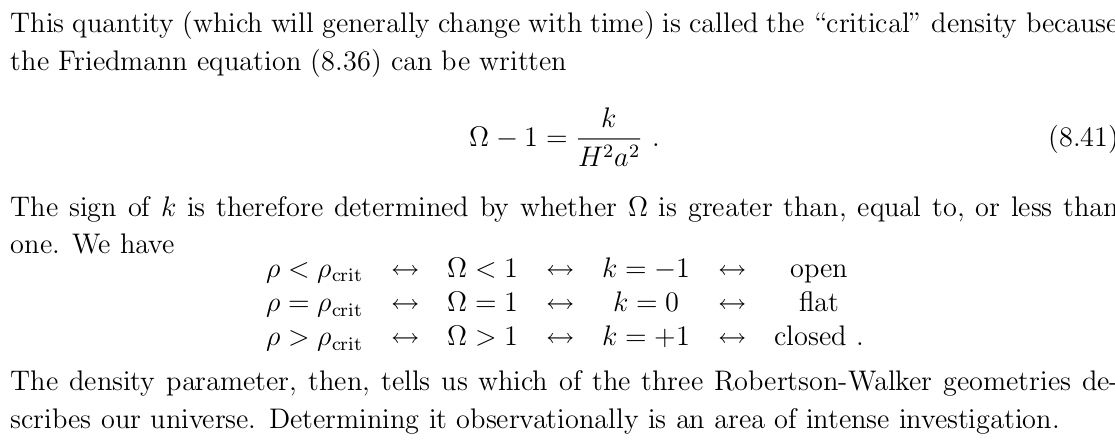
\includegraphics[width=0.7\linewidth]{gfx/criticaldensityCosomology}
	\caption{}
	\label{fig:criticaldensitycosomology}
\end{figure}

\subsubsection{On Killing Vectors in FLRW}
To understand how these quantities might conceivably be measured, let’s consider geodesic motion in an FLRW universe. There are a number of spacelike Killing vectors, but no timelike Killing vector to give us a notion of conserved energy. There is, however, a Killing
tensor. If $U^μ = (1, 0, 0, 0)$ is the four-velocity of comoving observers, then the tensor
\begin{equation} 
K\munu = a^2 (g\munu + U_μ U_ν )
\end{equation}
satisfies $∇_{(σ} K_{μν)} = 0$, and is therefore a \emph{Killing tensor}.Just as a Killing vector implies a constant of geodesic motion, if there exists
a Killing tensor then along a geodesic we will have
\begin{equation}
K_{\mu_1 \dots \mu_n} \frac{\md x^{\mu_1}}{\md \lambda } \dots \frac{\md x^{\mu_n}}{\md \lambda}=const.
\end{equation}
This means that
if a particle has four-velocity $V^μ = dx^μ /dλ$, the quantity
\begin{equation}
K^2= K\munu V^\mu V^\nu = a^2 \left[V^\mu V_\mu + (U_\mu V^\mu)^2\right]
\end{equation}
will be a constant along geodesics. Let’s think about this, first for massive particles. Then
we will have $V^μ V_μ = −1$, or
\begin{equation}
(V_0)^2 = 1 + g_{ij}V^i V^j = 1 + \abs{\vec{V}}^2.
\end{equation}
The Killing tensor then implies
\begin{equation}
\abs{\vec{V}} = \frac{K}{a}.
\end{equation}
The particle therefore “slows down” with respect to the comoving coordinates as the universe
expands. In fact this is an actual slowing down, in the sense that a gas of particles with
initially high relative velocities will cool down as the universe expands.\\
similar thing happens to null geodesics. In this case $V^2 = 0$, and $K^2=...$ implies
\begin{equation}
U_\mu V^\mu = \frac{K}{a}.
\end{equation}
But the frequency of the photon as measured by a comoving observer is $ω = −U^μ V_μ$ . The
frequency of the photon emitted with frequency $ω_1$ will therefore be observed with a lower
frequency $ω_0$ as the universe expands
\begin{equation}
\frac{\omega_1}{\omega_0} = \frac{a_0}{a_1}
\end{equation}
Cosmologists like to speak of this in terms of the redshift $z$ between the two events, defined
by the fractional change in wavelength:
\begin{equation}
z=\frac{\lambda_0-\lambda_1}{\lambda_1} = \frac{a_0}{a_1}-1.
\end{equation}
Notice that this redshift is not the same as the conventional Doppler effect; it is the expansion
of space, not the relative velocities of the observer and emitter, which leads to the redshift. But they´re are indistinguishable by Bartelmann, c.f. Cosmology section later. \todo{LOOK AT CAROLL PAGE 229 FOR INTERESTING DISTANCE MEASUREMENT TREATMENT IN COSMOLOGY SECTION}







\subsection{Comoving Coordinates Weinberg}
Imagine a finite region of space filled with a sen

\todo{Go through Comoving Coodinates on p338 by Weinberg to get a better notion of comoving coordinates and seperate its meaning from Rieamnnian normal coordiantes}



\subsection{Cosmological redshift- TO DO}
Assume both source and observer are comoving with the cosmic flow. Note that the adapted coordinates introduced before are the usual comoving coordinates :	



\newpage

\section{Friedmann models - A physical approach -- streamline with the above}
\subsection{Symmetry assumptions and consequences}
Cosmology rests on two fundamental assumptions
\begin{enumerate}
	\item When averaged over sufficiently large scales \footnote{Approximately $>200$Mpc.}, the observable properties of the universe are isotropic, i.e. independent of direction.
	\item Cosmological principles: Our position in the universe is by no means preferred to any other. The universe is spatially homogeneous.
\end{enumerate}
If the universe is isotropic around all of its points, it is also homogeneous.\\
Another assumption is that cosmology is described by general relativity. There, spacetime is a four-dimensional manifold whose metric tensor $g\munu$ is a dynamical field.\\
Rephrase the assumptions:
\begin{enumerate}
	\item 	When averaged over sufficiently large scales, there exists a mean motion of matter and energy in the universe with respect to which all observable properties are isotropic.\footnote{This is basically the comoving frame. I.e. the assumption says that there always exists a mean motion (i.e. a frame) under which spacetime appears to be isotropic.}
	\item All \textbf{fundamental observers}, i.e. imagined observers following this mean motion, experience the same history of the universe, i.e. the same averaged observable properties, provided they set their clocks suitably.	
\end{enumerate}
These assumptions translate into assumptions onto the metric of the underlying spacetime
\begin{enumerate}
	\item Time synchronization criterion \begin{equation}
		\abs{\md s}= c\md t,\quad g_{00} = - c^2.
	\end{equation}
	\item Required due to isotropy
	\begin{equation}
		g_{0i} = 0,\quad +\quad \abs{\md s}=c \md t.
	\end{equation}
	\item Because spacetime can be decomposed into spatial hypersurfaces of constant time, they can be scaled by a scale factor $a(t)$. I.e., the spacetime is described by the Robertson-Walker metric for a homogeneous and isotropic spacetime \ref{eq:metricRobertsonWalkerViaField}:
	\begin{align}
		\md s^2 &= g\munu \md x^\mu \md x^\nu = -c^2 \md t^2+a^2(t) \md l^2 \nonumber \\
		\md s^2 &= -c^2 \md t^2+ a^2(t) \left[\md w^2 + f^2_K(w) \md \Omega^2\right]
	\end{align}
Note here that $\md t$ is coordinate time, not the proper time. Further, with the normalization $a(t_0)=1$ we have that $\md l$ measures comoving distance, which is formally given by
\begin{equation}
\label{eq:conformaldistance}
	a \md \eta = - a \md \chi \quad \Rightarrow \; \chi = c \int_a^1 \frac{\md \tilde{a}}{\tilde{a}^2H(\tilde{a})},
\end{equation}
where $\eta$ is the \emph{conformal time}
\begin{equation}
	\label{eq:conformaltime}
	\md \eta = \frac{\md t}{a(t)}.
\end{equation}
\item Isotropy requires three-space to have spherical symmetry
\begin{equation}
	\md l^2 = \md w^2 + f^2_K(w) \left[\md \theta^2 + \sin^2 \theta \md \phi^2\right].
\end{equation}
\item Homogeneity requires
\begin{equation}
	f_K(w)= \left\{	\begin{array}{lll}
K^{-\half} \sin(\sqrt{K}w) & K>0 \\
w & K=0\\
\abs{K}^{-\half} \sinh(\sqrt{\abs{K}} w) & K<0\\
	\end{array}	\right\}
\end{equation}
with $K$ a constant ($[K]=cm^{-2}$) which parametrizes the curvature of spatial hypersurfaces.
\end{enumerate}
\subsubsection{Hubble law}
Note that we can expand the scale factor in a power series
\begin{equation}
	a(t_1) = a(t_0) \left[1+(t_1-t_0)H_0+\dots\right]
\end{equation}
which gives us the Hubble law for $z\ll 1$:
\begin{equation}
	z=H_0 (t_0-t_1)+\dots
\end{equation}
\subsection{Friedmann equations}
Einstein's field equations reduce to two DGL's for the scale factor $a(t)$, one equation from the time-time part and one from the three equal space-space parts of the field equations. The space-time and time-space part vanished due to our assumptions. 
\begin{mybox}{The first Friedmann equation}
	The first Fridmann equation reads
	\begin{align}
		\label{eq:friedmanneq1}
		\left(\frac{\dot{a}}{a}\right)^2 &= \frac{8 \pi \mG}{3 }\rho - \frac{K c^2}{a^2} + \frac{\Lambda c^2}{3} \nonumber \\
		\Leftrightarrow \quad H^2(t) &= H^2_0 \left[\Omega_{r,0} a^{-4} + \Omega_{m,0} a^{-3} + \Omega_{\Lambda,0} + \Omega_K a^{-2}\right]\nonumber \\
		&\equiv H^2_0 E^2.
	\end{align}
Note how all  density contributions in square brackets scale with different powers of $a$. Their relative importance thus changes over time. Today, the radiation density is much smaller than the matter density. Before a time $t_{eq}$ with
\begin{equation}
	a(t_{eq}) =: a_{eq} = \frac{\Omega_{r,0}}{\Omega_{m,0}}
\end{equation}
the universe is called \emph{radiation dominated}, $a_{eq} = 1.95 \cdot 10^{-4}$.
\end{mybox}
\begin{mybox}{Second Friedmann equation}
	\begin{align}
		\label{eq:friedmanneq2}
		\frac{\ddot{a}}{a} & = - \frac{4 \pi \mG}{3} (\rho + \frac{3 p}{c^2}) + \frac{\Lambda c^2}{3} \\
		&= H^2 +\dot{H} = - \half H^2_0 \left[\Omega_{m,0}a^{-3}-2 \Omega_{\Lambda,0}\right] \nonumber.
	\end{align}
A metric with a scale factor that satisfies \ref{eq:friedmanneq1},\ref{eq:friedmanneq2} is called \emph{Friedmann-Lemaitre-Robertson-Walker metric}.
\end{mybox}
\begin{mybox}{Adiabatic equation}
	\ref{eq:friedmanneq1} and \ref{eq:friedmanneq2} can be combined into the \emph{adiabatic equation} or the first law of thermodynamics without heat ($\delta Q=0$)
\begin{equation}
\frac{\md}{\md t}\overbrace{( a^3 \underbrace{\rho c^2}_{\epsilon})}^{\text{internal energy in volume }V=U} + p \frac{\md}{\md t}(\underbrace{a^3}_{V}) = 0,
\end{equation}
where $\rho,a,p$ are all functions of $t$. This equation intuitively states energy conservation:\\
The LHS is the change in internal energy, the RHS is the pressure work. The heat flow is absent because it would violate isotropy.
\end{mybox}



\subsection{Parameters}
\subsubsection{Pressure, density and equation of state}
With the energy density $\epsilon$ and the \emph{equation of state parameter} $\omega$, we can define the \emph{equation of state}
\begin{equation}
	p(t) = \omega \epsilon = \omega \rho(t) c^2,\quad \omega= \left\{		\begin{array}{lll}
\frac{1}{3} & \text{ ultra-rel. matter, i.e. fermion and bosonic}\\
0 &\text{non-rel. matter, thermal pressure is negligible}\\
-1 &\text{cosmic inflation, comoslogical constant, dark energy, vacuum}\\
	\end{array}	
	\right\}
\end{equation}
The pressure terms adds to the density because pressure is a consequence of particle motion, i.e. the kinetic energy of particles, which is equivalent to a mass density and thus acts gravitationally 
.\footnote{Cosmological constant can be interpreted as a type of matter, whose pressure is equal to its negative energy density.}
\footnote{Relativistic matter is what one calls radiation in cosmology and non-rel. matter is called dust.}
The adiabatic equation yields the density dependence on the scale factor:
\begin{equation}
	\rho(t)=\rho(t_0) a(t)^{-3(1+\omega)}.
\end{equation}
Consider the following equation of state parameters
\begin{enumerate}
	\item For non-rel. matter, $\omega=0$:\\
	\begin{equation}
		\rho_m(t)=\rho_{m,0}a^{-3}(t).
	\end{equation}
The density of non-rel. matter is decreasing because of dilution as space is expanding.
\item For radiation, $\omega=\frac{1}{3}$:\\
\begin{equation}
	\rho_r(t)=\rho_{r,0} a^{-4}(t),\qquad \lambda \propto a.
\end{equation}
The density of ultra-relativistic particles drops faster by one more power of $a$ because particles are diluted as space is expanding and lose energy as they are redshifted.
\item For dark energy, $\omega=-1$:\\
\begin{equation}
\rho \propto a^0.
\end{equation}
\end{enumerate}


\subsubsection{Density parameters and parameter values}
The density parameter $\Omega$ is defined as the ratio of the actual (or observed) density $\rho$ to the critical density $\rho_{cr}$ of the Friedmann universe. Then, $\rho_{cr}(t)$ is the critical density for which the spatial geometry is flat (or Euclidean).\\
\begin{mybox}{Density parameters}
With the critical density today $\rho_{cr,0}=1.86\times 10^{-29} h^2 g cm^{-3}$ corresponding to a galaxy mass per $Mpc^3$, we get
\begin{align}
	\Omega_r(t)&= \frac{\rho_{r,0}}{\rho_{cr}} a^{-4}(t)=\Omega_{r,0}a^{-4}(t),\\
	\Omega_m(t)&= = \frac{\rho_{m,0}}{\rho_{cr}} a^{-3}(t) = \Omega_{m,0} a^{-3}(t) \\
	\Omega_{\Lambda} (t) &= \frac{\Lambda c^2}{3 H^2(t)}\quad \text{with} \\
	\rho_{cr}(t)&= \frac{3 H^2(t)}{8 \pi \mG} \\
	\Omega_K &:= 1-\Omega_{r}-\Omega_{m}-\Omega_{\Lambda}= - \frac{K c^2}{H^2}.
\end{align}
\end{mybox}
Note that we therefore have
\begin{align}
	\rho_r(a)&= \Omega_{r,0} \rho_{cr,0} a^{-4},\\
	\rho_m(a) &= \Omega_{m,0} \rho_{cr,0} a^{-3}\\
	\Omega_r(a) &= \frac{\Omega_{r,0} a^{-4}}{E^2(a)}\\
	\Omega_{m}(a) &= \frac{\Omega_{m,0} a^{-3}}{E^2(a)}.
\end{align}
Two comments are in order:
\begin{enumerate}
	\item If $\Omega_{K,0} \approx 0$ today, then it is even more negligible going back in time, as $\Omega_r,\Omega_m$ dominate past $\Omega_K$ by far.
	\item What does $\rho_{cr}(t)$ represent ? We can bring it into the following form:
	\begin{equation}
		\rho_cr(t) = \dots \; \Leftrightarrow \; \frac{4 \pi \mG}{3} \left(\frac{\rho_{cr} a^3}{a}\right) = \frac{\dot{a}^2}{2}.
	\end{equation}
	From this we can read off the following interpretation: ’A sphere whose matter is completely filled with critical density has the property, that its kinetic energy exactly equals out the potential energy per particle.’
\end{enumerate}
\begin{mybox}{Hubble parameter}
	The \emph{Hubble parameter} is defined as the relative expansion rate 
	\begin{equation}
	\label{eq:hubbleparameter}
	H(t):= \frac{\ddot{a}(t)}{a(t)}
	\end{equation}
	with the \emph{Hubble constant}
	\begin{equation}
		\label{eq:hubbleconstant}
		H(t_0)=: H_0 = 100 h \;\frac{km}{s Mpc} = 3.22\times 10^{-18} h \; s^{-1}.
	\end{equation}
	It quantifies by how much the \emph{recession velocity} of cosmic objects grows as their distance increases. \textbf{Every length scale changes by $H_0$ per second}.
\end{mybox}
The \emph{Hubble time} is
\begin{equation}
	t_H = \frac{1}{H_0} = 9.82 \times 10^9 \frac{yr}{h} \approx 15 Gyr.
\end{equation}
The \emph{Hubble radius} is
\begin{equation}
	r_H=\frac{c}{H_0} = 3.01 \times 10^3 \frac{Mpc}{h} \approx 5 Gpc.
\end{equation}
\begin{mybox}{Evolution of epochs}
	 \begin{tabular}{|l|llll|}
		          & $\omega$ & $\rho(a)$ & $a(t)$ & $a(\tau)$ \\
		\toprule
		\text{radiation dominated, RD} & $\frac{1}{3}$&$a^{-4}$&$t^{\half}$ & $\tau$ \\
		\text{Matter dominated, MD} & $0$ & $a^{-3}$ & $t^{\frac{2}{3}}$ & $\tau^2$ \\
		$\Lambda$\text{ dominated, $\Lambda$D} & $-1$ & $a^0$ & $e^{H_0 \sqrt{\Omega_{\Lambda,0} t} }$ &$-\tau^{-1}$\\
		\bottomrule
	\end{tabular}
\end{mybox}
\begin{figure}[h!]
	\centering
	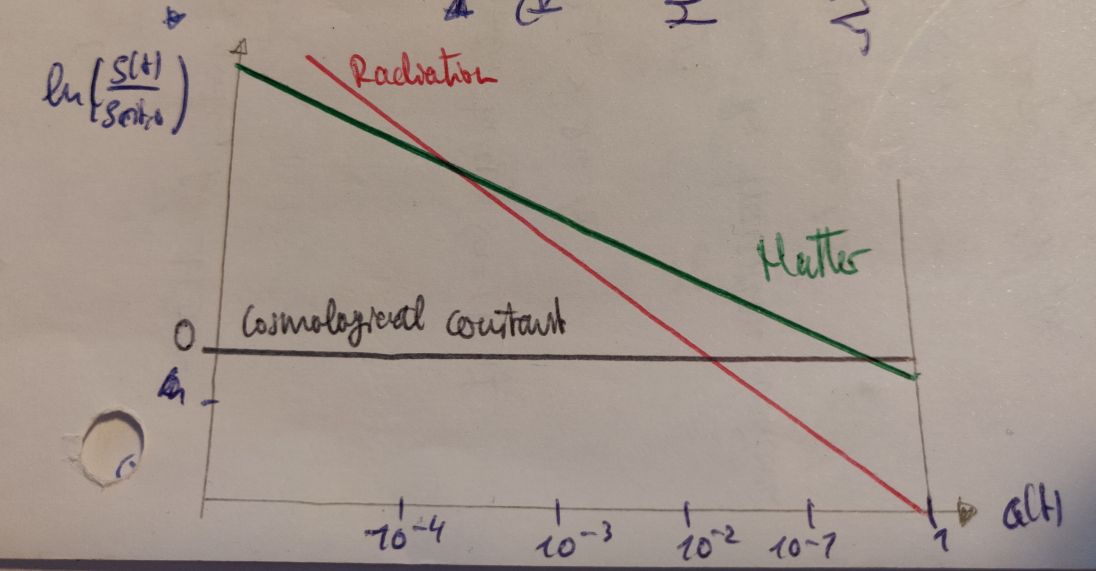
\includegraphics[width=0.7\linewidth]{gfx/EvolutionEpochs}
	\caption{}
	\label{fig:evolutionepochs}
\end{figure}
\subsection{Redshift (cosmological)}
\subsubsection{Role of the observer - Definitions}
\begin{mybox}{Comoving observer}
	A \emph{comoving observer} is the only observer that will perceive the universe (e.g. CMB) as isotropic. Non-comoving observers will see regions of the sky systematically blue-or redshifted.\\
	Thus, isotropy in particular defines (especially isotropy of the CMB) a special local frame of reference called the \emph{comoving frame}.  \emph{Cosmic time} is then the time in the comoving frame.
\end{mybox}
\begin{mybox}{Comoving frame - coordinate system}
	Comoving coordinates assign constant spatial coordinate values to observers who perceive the universe as isotropic, hence comoving observers. We are considering the dynamics of particles
	on an expanding spatial background, the physical distance $\vec{r}$ between any two particles
	therefore grows with time in proportion to the scale factor $a ( t )$ , i.e. comoving coordinates $q$ are defined via the spatial coordinates as
	\begin{equation}
		\label{eq:comovingcoordinates}
		\vec{r}(t) = a(t) \vec{q}.
	\end{equation}
\end{mybox}
\begin{mybox}{Velocities}
	The velocity of an observer relative to the local comoving frame is called \emph{peculiar velocity} of the observer. It therefore is the component of an e.g. galaxy' s velocity that deviates from the \emph{Hubble flow} (i.e. \emph{the motion solely due to the expansion of space}). \\
	\emph{Recession velocity} is then the rate at which an astronomical object is moving away (e.g. from Earth).
\end{mybox}

\subsubsection{Redshift definition}
\begin{mybox}{Redshift}
Spatial hypersurfaces can expand or shrink by the scale factor $a(t)$. This leads to a red- of blueshift of photons propagating through spacetime
\begin{equation}
	\ref{eq:redshiftCosmo}
	\frac{a(t_{\text{observed}})}{a(t_{\text{emitted}})} \stackrel{ a(t_0)\stackrel{!}{=}1}{=} \frac{1}{a(t_e)} = 1+z = \frac{\lambda_0}{\lambda_e} = \frac{\nu_e}{\nu_0},\quad a(t_e)\equiv a.
\end{equation}\end{mybox}
Comments:
\begin{enumerate} 
	\item Derivation of the above:
This stems from the fact that for light we have
\begin{equation}
	\md s^2 =0 =-c^2 \md t^2+a^2 \md \omega^2\; \Leftrightarrow \; c\abs{\md t} = a(t) \md \omega,
\end{equation}
as light has a vanishing proper time. Now consider light emitted from a comoving source at time $t_e$ reaching a comoving observer at $\omega=0$ at time $t_o$; hence the coordinate distance between the source and observer is
\begin{equation*}
\omega_{e,o} = \int_{t_e}^{t_o} \md \omega = \int_{t_e}^{t_o}  \frac{c \md t}{a(t)} = const.
\end{equation*}
as the source and observer are both comoving. Then
\begin{equation*}
0 \stackrel{!}{=} \frac{\md \omega_{e,o}}{\md t} \; \Rightarrow \; \frac{\md t_o}{\md t_e} = \frac{a(t_o)}{a(t_e)} \Leftrightarrow \; \tau_e=\tau_o.
\end{equation*}
\item 
\end{enumerate}
\subsubsection{Big Bang}
The \emph{relative acceleration} $\frac{\ddot{a}}{a}$ is given, for $\Lambda$CDM Universe and pressure-less matter, as
\begin{equation}
\frac{\ddot{a}}{a} = H^2_0 \left[\Omega_{\Lambda,0}-\frac{\Omega_{m,0}}{2 a^3}\right].
\end{equation}
The expansion of the universe therefore accelerates today ($a=1$) if
\begin{equation}
\ddot{a} = H^2_0 \left[\Omega_{\Lambda,0}-\frac{\Omega_{m,0}}{2}\right]>0 \text{ or if } \Omega_{\Lambda,0} > \frac{\Omega_{m,0}}{2}.
\end{equation}
The latter if-statement is rendered true by measurements. Thus, \textbf{the Universe's expansion accelerates today}.\\
If the Universe indeed is spatially flat, then the transition between decelerated and accelerated expansion happened at
\begin{equation}
	1-0.263 \approx \frac{0.263}{2 a^3} \Rightarrow a = 0.56, \; z=0.78.
\end{equation}
Luminosity distances to supernovae at larger redshifts show this transition.
\subsection{Age and Expansion of the Universe}
The age of the universe can be calculated by 
\begin{equation}
	t= \int_{a(z_1)}^{a(z_2)} \frac{\md a^\prime}{a^\prime H(a^\prime)} = \frac{1}{H_0} \int_{a(z_1)}^{a(z_2)} \frac{\md a^\prime}{a^\prime E(a^\prime)}, \quad z_1>z_2
\end{equation}
setting $a(z_1)=0, a(z_2)=a$. This integral can only be solved analytically via approximations/assumptions:
\begin{enumerate}
	\item For a flat, single component universe (where the e.o.s. parameter does \emph{not} change over time), the Friedmann eq. reduces to
	\begin{equation*}
		H = H_0 \sqrt{\Omega_{I,0}} a^{-\frac{3}{2} (1+\omega_I)},
	\end{equation*}
	thus
	\begin{equation}
	a(t) \propto \left\{ \begin{array}{lll}
	t^{\frac{2}{3}(1+\omega_I)} & w_I\neq -1,&a(t)\propto \begin{array}{ll}
	t^{\frac{2}{3}} & \text{MD} \\
	t^\half & \text{RD}\\
	\end{array}		\\
	e^{H_0 \sqrt{\Omega_I} t} & \omega=-1 & \Lambda\mathrm{D}.	\end{array}\right\}
	\end{equation}
\item Einstein-deSitter: $\Omega_{r,0}=\Omega_{\Lambda,0}=0$,$\Omega_{m,0}=1,\Omega_{K,0}=0$ $\Rightarrow E(a) \approx \sqrt{\Omega_{m,0}} a^{-\frac{3}{2}}$
\begin{equation}
	t = \frac{2}{3} \frac{a^{\frac{3}{2}}}{H_0} \; \Rightarrow \; t_0 = \frac{2}{3 H_0}, \; \Leftrightarrow \; a=\left[\frac{3}{2} H_0 t\right]^{\frac{2}{3}} \propto t^{\frac{2}{3}}.
\end{equation}
This describes the universe well for $z\in [2,300]$.
\item Early Universe:
\begin{equation*}
	E(a) \approx \sqrt{\Omega_{r,0} a^{-4}+\Omega_{m,0} a^{-3}},
\end{equation*}
\begin{equation}
	\Rightarrow \; t(a=a_{eq}) = t_{eq} = \frac{2 a^{\frac{3}{2}}_{eq} }{3 H_0 \sqrt{\Omega_{m,0}}} (2-\sqrt{2}) \approx 20.000 yr \rightarrow \footnote{including neutrino partake in $\Omega_{r,0}$} 50.000 yr.
\end{equation}
The radiation dominated epoch is thus very short compared to the age of the universe. Therefore, for the most part of the cosmic time, radiation is negligible because the period of radiation domination is very brief in comparison.
\item Very later universe: $E(a)\approx \sqrt{\Omega_{\Lambda,0}}$
\begin{equation}
	\Rightarrow \quad t = \frac{\ln(a)}{H_0 \sqrt{\Omega_{\Lambda,0}}} \; \Rightarrow \; a \propto \exp\left[\sqrt{\Omega_{\Lambda,0}} H_0 t\right].
\end{equation}
Here the universe expands forever exponentially (\emph{deSitter limit}). A universe expanding with $H_0$ today may never reach $a=0$ going back in time. The fact that the universe is expanding today does thus not imply that it originated in a Big Bang. There must have been a Big Bang though, because:
\begin{enumerate}
	\item From existence of the CMB we know that radiation density is finite.
	\item From the existence of luminous material that the matter density is finite.
	\item From existence of objects with $z\gg 0$ we know that $a(z)$ must have been as small as $\frac{1}{1+z}$ or smaller in the past.
\end{enumerate}
\item ODM: $K\neq =,\Omega_{m,0} \neq 0, \Omega_{\Lambda,0}=0$.
\end{enumerate}

\subsection{Distance measures}
In general, $z$ is the only observable in cosmology (via comparison of absorption/emission lines e.g.). All distances are therefore expressed in terms of the redshift.\\
An object at higher redshift $z_2$ is more distant to us than one at $z_1 < z_2$. The more distant a source is from us, the longer the light takes to reach us, the earlier it was emitted, the smaller $a$ was at emission, ant the larger $z$ is.
\subsubsection{Proper distance - not observable}
The distance measured by the time required for light to travel from a source to an observer
\begin{mybox}{Proper distance}
	\begin{equation}
		\md D_{prop} =-c \md t,\; \Rightarrow\;	D_{prop}(z_1,z_2)= \frac{c}{H_0} \int_{a(z_2)}^{a(z_1)} \frac{\md a}{a E(a)},
	\end{equation}
	thus the distance increases as we move away from observer (therefore minus sign).
\end{mybox}
This distance changes in time and therefore has to be done about two points $z_1,z_2$ with the same cosmological time. $D_{prop}$ is what a measurement at constant cosmic time would yield.
\subsubsection{Comoving distance - not observable}
The distance on the spatial hypersurface at $t=const.$ between the world lines of a source comoving with the mean cosmic flow, thus the comoving distance accounts for the expansion of the universe. $D_{com}$ is obtained by integrating the proper distance of nearby fundamental observers along the line of sight.
\begin{mybox}{comoving distance}
	For objects moving (only) with the Hubble flow, it is deemed to remain constant in time
	\begin{equation}
		D_{com}(z_1,z_2) = \int_{a(z_2)}^{a(z_1)} \md \omega= \frac{c}{H_0} \int_{a(z_1)}^{a(z_2)} \frac{\md a}{a^2 E(a)} =: \omega(z_1,z_2).
	\end{equation}
	Another form for photons in particular (i.e. $\md s=0$, $a \md\omega=-c \md t$) $t_e$ the time of emission of photons detected by the observer and $t$ is present
	\begin{equation}
	\omega=	c \int_{t_e}^t \frac{\md t^\prime}{a(t^\prime)}.
	\end{equation}
\end{mybox}
This is the distance one acquires for solely moving with the Hubble flow. Thus dividing by $a$ scales back to initial distance, which will be constant if observer and emitter are both only moving with the Hubble flow.

\begin{figure}[h!]
	\centering
	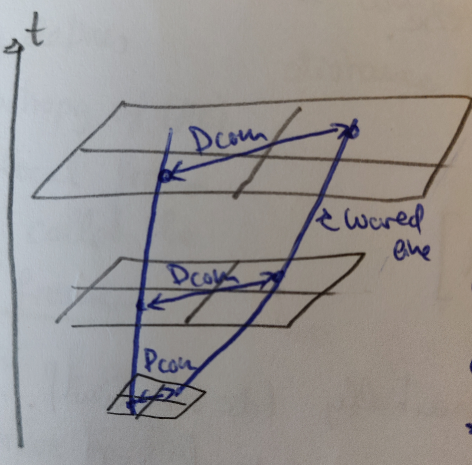
\includegraphics[width=0.7\linewidth]{gfx/comovingdistance}
	\caption{}
	\label{fig:comovingdistance}
\end{figure}





\subsubsection{Angular diameter distance}
If you know the are of the observed source $\delta A$ and measure the solid angle $\delta \Omega$ under which it appears, then you get the distance from the source to an observer via the comoving distance
\begin{equation}
	D_{ang}(z_1,z_2) = \sqrt{\frac{\delta A}{\delta \Omega}} = \frac{a(z_2)}{a(z_1)} f_K\left[D_{com}(z_1,z_2)\right].
\end{equation}
$D_{ang}$ is measured on the backward lightcone. The backward lightcone itself shrinks due to the expansion of space. Therefore, the angular size of an object changes non-monotonic w.r.t. the distance. This is due to the four-dimensional curvature of spacetime, which resolves in a focussing effect on most distance source. We therefore perceive them as being near us (by means of angular diameter distance).

\begin{figure}[h!]
	\centering
	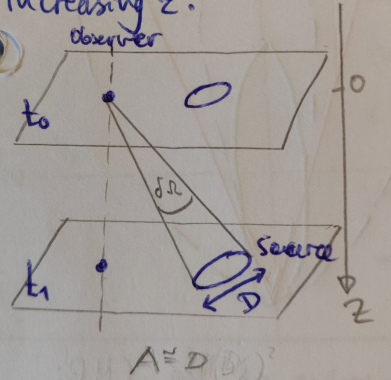
\includegraphics[width=0.7\linewidth]{gfx/AngulardiameterDistance}
	\caption{}
	\label{fig:angulardiameterdistance}
\end{figure}





$D_{ang}$ has maximum at $z=\frac{5}{4}$ in Einstein-deSitter universe and gently decreases for increasing $z$.

\begin{figure}[h!]
	\centering
	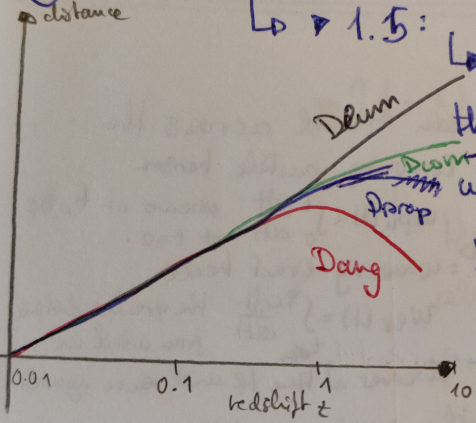
\includegraphics[width=0.7\linewidth]{gfx/DistancemeasuresCompared}
	\caption{}
	\label{fig:distancemeasurescompared}
\end{figure}

\subsubsection{Luminosity distance and Etherington relation}


\begin{figure}[h!]
	\centering
	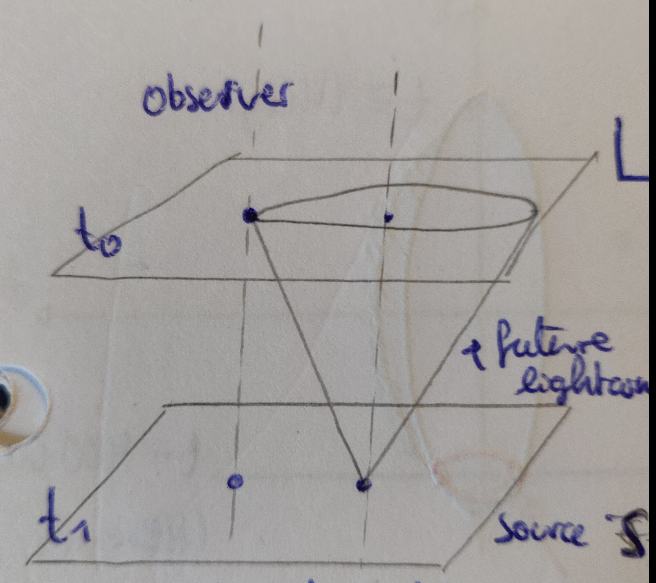
\includegraphics[width=0.7\linewidth]{gfx/AngulardiameterDistance1}
	\caption{}
	\label{fig:lumininositydistance1}
\end{figure}
For a source with bolometric luminosity $L$ and flux $S$ (i.e. at the source we have $S=\frac{L}{4 \pi d^2}$)
\begin{equation}
	D_{lum}(z_1,z_2) = \sqrt{\frac{L}{4 \pi S}}.
\end{equation}
\begin{mybox}{Etherington relation}
\begin{equation}
	D_{lum}(z_1,z_2) = \left[\frac{a(z_1)}{a(z_2)}\right]^2 D_{ang}(z_1,z_2) = (1+z)^2 D_{ang},
\end{equation}
where the latter equality holds for $z_1=0$ for observer (usually true as we mostly have measurements in the present time on Earth) and $z_2=z$ for emission/source.
\end{mybox}
Photons are therefore redshifted by $\frac{a_1}{a_2} >1$ between emission and absorption, their arrival times are strecthed by $\frac{a_1}{a_2}$ and they are spatially diluted by factor $\left(\frac{a_1}{a_2}\right)^2$, thus $L\propto \left(\frac{a_1}{a_2}\right)^4 S$. Therefore, the Etherington relation gives the scale factor between the shrinking backward lightcone and forward lightcone.
\\
\\
To recapitulate, the Angular diameter distance is a measurement on the backward lightcone (compare \ref{fig:angulardiameterdistance}). The luminosity distance is exactly the opposite (compare \ref{fig:lumininositydistance1}). The flux is the section we receive from the source, compare \ref{fig:luminositydistance}.
\begin{figure}[h!]
	\centering
	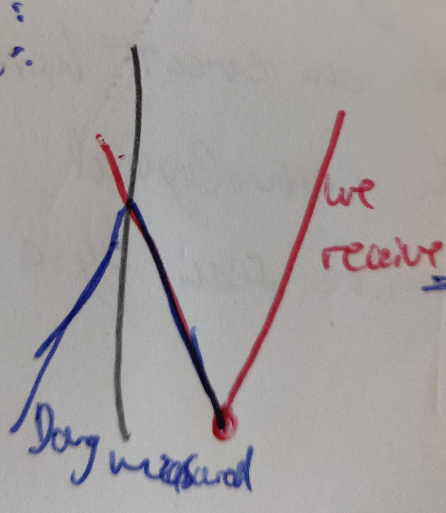
\includegraphics[width=0.7\linewidth]{gfx/luminositydistance}
	\caption{}
	\label{fig:luminositydistance}
\end{figure}
\newpage
\subsection{Horizons}
Horizons occur because of the finite speed of light and the expansion of the Universe:
\begin{enumerate}
	\item There exists a \emph{particle horizon}, i.e. light can only travel by a finite distance between the Big Bang and any later time, thus any particle in the universe can only be influenced by events within a finite region.
	\item There exists an event horizon if the expansion of the universe is dominated by the cosmological constant at late times. Then, the region which can be seen by a particle remains finite.
\end{enumerate}
Formulate these horizons in explicit terms.\\
Between times $t_1$ and $t_2 > t_1$, light can travel across the comoving distance
\begin{equation}
	\Delta \omega(t_1,t_2)= \int_{t_1}^{t_2} \frac{c \md t}{a(t)} = \frac{c}{H_0} \int_{a(t_1)}^{a(t_2)} \frac{\md a^\prime}{{a^\prime}^2 E(a^\prime)}.
\end{equation}
This gives us two different kinds of horizons.
\begin{mybox}{Horizons}
	\begin{enumerate} 
		\item 
	\emph{Comoving particle horizon}
	\begin{equation}
		\omega_{ph}(t)=\int_0^t \frac{c \md t}{a(t)}
	\end{equation}
	with observer at $t$ and Big Bang at $t=0$.
	\item \emph{Comoving event horizon}
	\begin{equation}
		\omega_{eh} (t) = \int_t^{t_f} \frac{c \md t}{a(t) }
	\end{equation}
	which is the greatest possible distance from which an observer at time $t_f$ will receive signals.
\end{enumerate}
\textbf{Altogether, the region that we perceive (particle horizon) is finite and the region we can influence (event horizon) is finite}.
\end{mybox}
\textbf{Our backward lightcone is all of the universe we can see, a tiny fraction of the actual universe.}
\begin{figure}[h!]
	\centering
	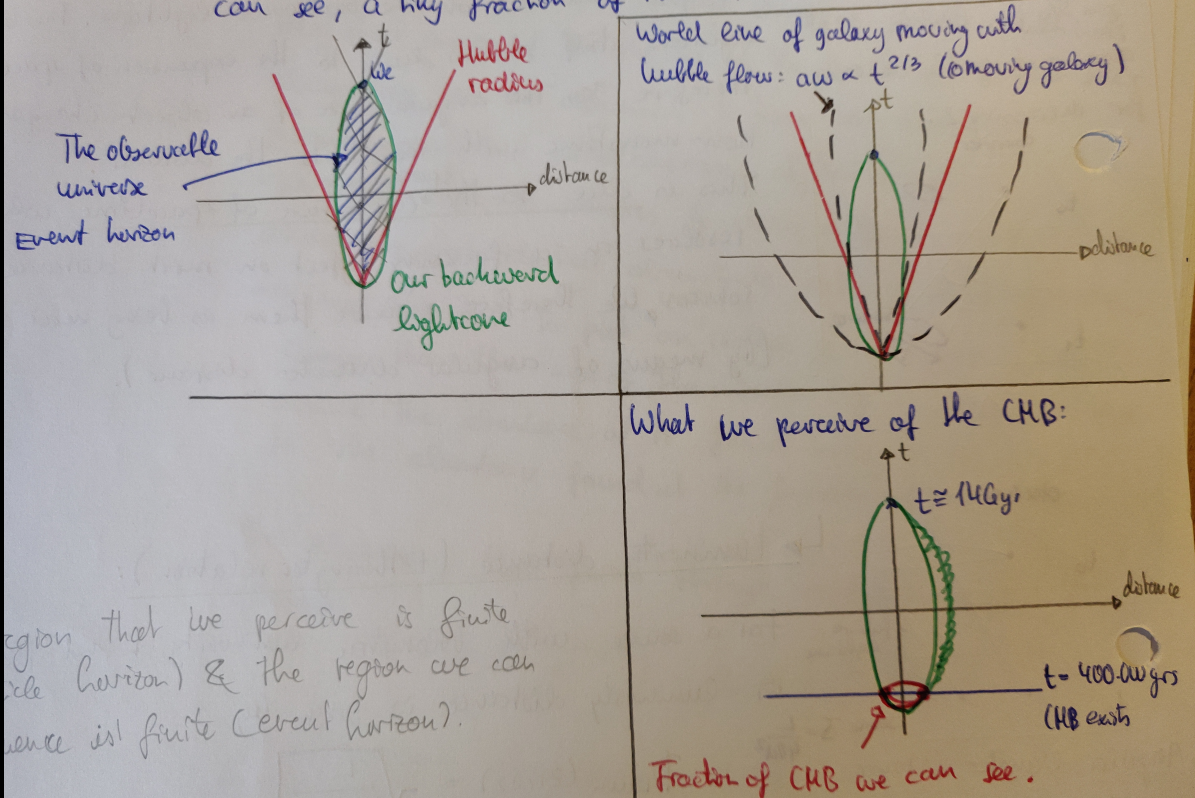
\includegraphics[width=0.7\linewidth]{gfx/Horizons}
	\caption{}
	\label{fig:horizons}
\end{figure}


















\section{Age of the Universe and the cosmic expansion}
\subsection{Nuclear cosmo-chronology}
\subsection{Stellar ages}
\subsection{Cooling of white dwarfs}
\subsection{The Hubble constant}
\subsection{Supernovae of type Ia}




\section{Thermal evolution of the universe}
\subsection{Assumptions and quantum statistics}
\subsubsection{Assumptions}
The underlying assumptions are
\begin{enumerate}
\item \emph{The universe expands adiabatically}-\\
isotropy requires the universe expand adiathermally: no heat can flow because flow directions would violate isotropy. Adiathermal expansion is adiabatic if it is reversible, thus if entropy does not change. Entropy does indeed changed, but, because of $\frac{n_{\text{Baryon}}}{n_\gamma} \approx 10^{-9}$, the entropy from electromagnetic radiation of the CMB dominates the entropy of the universe by far $\Rightarrow$ entropy generations completely negligible.
\item \emph{Thermal equilibrium can be maintained despite the expansion} $\Leftrightarrow$ At very early times, there was thermal equilibrium between interacting particle species-\\
thermal equilibrium can only be maintained if the interaction rate of particles is higher than the expansion rate of the Universe. For $t\rightarrow0$, particle densities grow so fast that interaction rates are indeed higher than the high expansion rates at early times. As the universe proceeds to expand, now and then then single particle species will fall out of thermal equilibrium.\\
\\ From the perfect black-body spectrum of the CMB we have good observational evidence that the early universe was in local thermal equilibrium. This perfect planck black-body spectrum also implies that the universe was in thermal equilibrium during decoupling and even so later on. Particles maintain thermal equilibrium due to direct collisions (Thomson scattering). The thermal equilibrium disappears, because energies of particles and scattering cross sections become very low. This is because the mean free path becomes very large, i.e. interactions/collisions are not very likely to happen.
\item \emph{The cosmic ’fluids’ can be treated as ideal gases}- \\
thus there are no long-range interactions between particles, they can only interact by direct collisions. Holds also for charged particles, because oppositely charged particles shield each other.\footnote{Note that for charged particles, the Couloum-potential goes like Yukawa-potential, i.e. has an exponential cut-off. Therefore, this is a valid approximation.}
\end{enumerate}

\subsubsection{Recap on quantum statistics}
\begin{enumerate}
	\item The ensemble is \emph{canonical}, if the mean internal energy is specified. I.e. Helmholtz free energy
	\begin{equation}
		F=-k_B T \ln(Z_c),\quad Z_c=\sum_\alpha \exp[-\frac{\epsilon_\alpha}{k_B T}]
	\end{equation}
	with $Z_c$ the canonical partition sum over all accessible quantum states.
	\item The ensemble is \emph{grand-canonical}, if only the mean number of particles is specified. This transitions to the grand-canonical potential
	\begin{equation}
		\mJ = - k_B T \ln(Z_{gc})
	\end{equation}
	with the gc partition sum $Z_{gc} = \prod_\alpha Z_\alpha$ with
	\begin{equation}
		Z_\alpha = \sum_{N_\alpha} e^{-(\epsilon_\alpha-\mu) \frac{N_\alpha}{k_B T}} = \left\{	\begin{array}{ll}
	1+e^{-\frac{(\epsilon_\alpha-\mu)}{k_B T}} & \text{fermions} \\
	1-e^{-\frac{(\epsilon_\alpha-\mu)}{k_B T}} & \text{bosons} \\
		\end{array}		\right\}.
	\end{equation}
	By 
	\begin{equation}
		N_\alpha = \left\{ \begin{array}{ll}
		0,1 & \text{fermions} \\
		0,1,\dots,\infty & \text{bosons} \\
		\end{array}			\right\}
	\end{equation}
	it follows that the mean occupation number of a quantum state $\alpha$ is
	\begin{equation}
		\bar{N}_\alpha= \frac{1}{e^{\frac{\epsilon_\alpha-\mu}{k_B T}} \pm 1}, \quad \begin{array}{ll}
		+ & \text{fermions}\\
		- & \text{bosons, diverges for Bose Condensation}\\
		\end{array}.
	\end{equation}
	The spatial number density in thermal equilibrium is
	\begin{equation}
		n = \sum_\alpha N_\alpha = \int \md N = \int g \frac{V}{(2\pi)^3} \md^3 p = \int \frac{\md^3 p}{(2 \pi)^3} \frac{g}{e^{\frac{\epsilon(p)}{k_B T} }\pm 1},
	\end{equation}
	with $g$ being the statistical weight, i.e. $g_\gamma=2$ for photons and otherwise $g=2s+1$ for spin-$s$ particles, and with 
	\begin{equation}
		\epsilon(p) = \left\{\begin{array}{ll}
		cp & \text{ultra-rel. gas} \\
		\sqrt{c^2 p^2+m^2c^4} & \text{rel. gas} \\
		\frac{p^2}{2m} & \text{non-rel. gas} \\
		\end{array}		\right\}.
	\end{equation}
	Thus, the mean energy density in thermal equilibrium is
	\begin{equation}
	U = \int \pmeasure \frac{g \epsilon(p)}{e^{\frac{\epsilon(p)}{k_B T}} \pm 1 }.
	\end{equation}
\footnote{$1eV=1.6\times 10^{-12}erg$, i.e. $k_B T = 1.16\times 10^4 K$.}
	\begin{mybox}{Ultra-rel. boson in thermal equilibrium}
		\begin{align}
			N_B &= g_B \frac{\zeta(3)}{\pi^3} \left(\frac{k_B T}{\hbar c}\right)^3 \quad \propto T^3\\
			U_B &= g_B \frac{\pi^2}{30} \frac{(k_B T)^4}{(\hbar c)^3}\quad \propto T^4\\
			P_B &= \frac{1}{3} U \quad \propto T^4\\
			S_B &= g_B k_B \frac{2 \pi^2}{45} \left(\frac{k_B T}{\hbar c}\right)^3 \quad \propto T^3.
		\end{align}
	\end{mybox}
\begin{mybox}{Ultra-rel. fermions in thermal equilibrium}
	\begin{align}
		n_F &= \frac{g_F}{g_B} n_B=\frac{3}{4} n_B \quad \propto T^3\\
		u_F &= \frac{7}{8} u_B \quad \propto T^4\\
		P_F &= \frac{g_F}{g_B} P_B=\frac{7}{8} P_B \quad \propto T^4 \\
		S_F &= \frac{3}{4} S_B \quad \propto T^3.
	\end{align}
\end{mybox}
\item For non-rel. classical gas we acquire the Maxwell-Boltzmann distribution
\begin{align}
n&= \left(\frac{m k_B t}{2 \pi^2 \hbar^2}\right)^\frac{3}{2} \exp\left[-\frac{mc^2}{k_B T}\right]\\
u&=c_V n = \frac{f}{2} n k_B T,\\
P&= nk_B T.
\end{align}\footnote{By comparing the rel. limit $k_B T \gg mc^2$, we see that the number density, energy density, and pressure of a particle species fall exponentially (are "\emph{Boltzmann suppressed}") as the temperature drops below the mass of the particles.}
\end{enumerate}
Note that the \emph{chemical potential} $\mu$ encodes what it costs to move, i.e. $\partial_N U$ one particle from one place to another. The chemical potential characterizes the response of a system to a change in particle number
\begin{equation}
\label{eq:chemicalpotential}
	\mu = - T \left(\frac{\partial S}{\partial N}\right)_{U,V}.
\end{equation}
The second law of thermodynamics means that particles flow to the side of the reaction with the lower total chemical potential. Chemical equilibrium is reached when the sum of the chemical potentials of the reacting particles is equal to the sum of the chemical potentials of the products. The rates of the forward and reverse reaction are then equal.
\subsubsection{Adiabatic expansion of ideal gas}
In thermal equilibrium we have
\begin{enumerate}
	\item For rel. boson or fermion gases, we have $P=\frac{u}{3}= \frac{E}{3V}$
	\item For non-rel. gases $U = \half f N k_B T$.
\end{enumerate}
By the first law of thermodynamics in absence of heat transfer $\md E + P\md V=0$ we find
\begin{equation}
T\propto \left\{\begin{array}{ll}
V^{-\frac{1}{3}} \propto a^{-1} & \text{rel. boson or fermion gas }\gamma=\frac{4}{3} \\
V^{-\frac{5}{3}+1} \propto a^{-3(1-\gamma)} \propto a^{-2} & \begin{array}{ll}
\gamma=\frac{5}{3}&\text{non-rel 1-atomic, ideal gas } \\
\gamma=\frac{9}{7}& \text{ for diatomic molecule}\\
\end{array}
\end{array}			\right\}.
\end{equation}
Therefore the temperature of non-rel. gases drops faster with the expansion of the universe. Further on we see that the temperature of things in the universe will be maintained equally early on, but will differ more and more with expansion.\\
For non-rel. gases we have to consider the explicit degree of freedom

	 \begin{tabular}{|l|llll|}
	& $\bullet$ & $2$-atomic identical (3 transl.$+2$ rot.) & $2$-atomic non-identical ($3$ transl. $+4$ rot..) \\
	\toprule
$\gamma$ &$\frac{5}{3}$ & $\frac{7}{5}$ & $\frac{9}{7}$\\
$f$ & $3$ & $5$ & $7$ \\
	\bottomrule
\end{tabular}
thus
\begin{equation}
	T\stackrel{\stackrel{f\rightarrow\infty}{\gamma \longrightarrow 1}}{\longrightarrow} constant.
\end{equation}



\subsubsection{Particle freeze out}
At early times (radiation-dominated era) the expansion time-scale is
\begin{equation}
	t_{exp} \approx \frac{1}{\sqrt{\mG \rho}}\propto a^2.
\end{equation}
The expansion time-scale (e.g. time-scale for universe to double its radius) is very brief thus increases rapidly as the universe expands away from the Big Bang.\\
\\
Whether the assumption of thermal equilibrium is valid is shown by comparison of expansion rate of the universe to the interaction rate of particles.\\
Thermal equilibrium is maintained predominantly by two-body interactions. The collision rate is, where $n\propto T^3$ for rel. particles, 
\begin{equation}
	\Gamma:= \frac{\md N}{\md t}= n \expval{\sigma v} \propto n \propto T^3 \propto a^{-3}. 
	\end{equation}
	\footnote{In the second step we used: For a process like $1+2\leftrightarrow 3+4$ we would write the interaction rate of species $1$ as $\Gamma_1=n_2 \sigma v$, where $n_2$ is the density of the target species $2$ and $v$ is the average velocity of $1$ and $2$. The interaction rate of species $2$ would be $\Gamma_2=n_1 \sigma v$. We have used the epxectation that at high energies $n_1 \approx n_2 \equiv n$.}
This shows that different particle species may have different interaction rates and so may decouple at \textbf{different times}.\\
The collusion time scale is thus
\begin{equation}
	t_{coll} = \Gamma^{-1} \propto a^3.
\end{equation}
\begin{mybox}{Validation of thermal equilibrium assumption}
Thus
\begin{equation}
	\frac{t_{exp}}{t_{coll}} \propto a^{-1} \stackrel{a\rightarrow 0}{\longrightarrow} \infty,
\end{equation}
which implies that the collisions have a much shorter time scale than the expansion in the early universe. Thermal equilibrium can thus be maintained despite the expansion in particular at early times. As the universe keeps expanding, collisions become rare and thermal equilibrium will ultimately break down.
\end{mybox}
The continuity equation of particle numbers in the universe is regulated by the destruction through collisions (i.e. $\Gamma$) and by thermal creation ($n_T=$ thermal number density, creation due to e.g. collisions).\\
In the absence of interactions, it reads per particle species $i$
\begin{equation}
\frac{\md n_i}{\md t} + 3 \frac{\dot{a}}{a} n_i=0.
\end{equation}
\begin{mybox}{Freeze-out or Boltzmann equation}
Noting $\Gamma_1=n_2 \expval{\sigma v}$ and introducing the comoving number density $N=a^3n$, we find from this continuity equation
\begin{equation}
\frac{\md \ln N_1}{\md \ln a} = - \frac{\Gamma_1}{H(a)}\left[1 -\frac{N^2_{T,1}}{N^2_1}\right] =\begin{array}{ll}
\frac{\md \ln N}{\md \ln a}>0 & N<N_T\\
\frac{\md \ln N}{\md \ln a} <0 & N>N_T\\
\end{array},
\end{equation}
such that for $N<N_T$ there are more particles produced until $N=N_T$ whereas for $N>N_T$ particles get destroyed in order to get back to $N=N_T$.\\
Overall, no matter the initial conditions, the thermal number will be established for frequent collision rates and $N\gg0$.
\end{mybox}
\footnote{On the freeze-out equation: For $\Gamma_1\gg H$ the natural state of the system is chemical equilibrium. Imagine that we start with $N_1 \gg N_{1,T}$. The RHS then is negative, particles of type $1$ are destroyed and $N_1$ is reduced towards the equilibrium value $N_{T,1}$. Similarly, if $N_1\ll N_{1,T}$, the RHS is positive and $N_1$ is driven towards $N_{1,T}$. As long as the interaction rates are large, the system quickyl relaxes to a steady state where the RHS vanishes and the particles assume their equilibrium abundances. Thus, ’\textbf{with interaction rates high, particles retain the equilibrium state}’. When the reaction rate drops below the Hubble scale $\Gamma_1 <H$, the RHS gets suppressed and the comoving density of particles approaches a constant relic density, i.e. $N_1=$constant.}
About the freeze out equation:\\
If $N=N_T$, it does not change. If $N$ deviates from $N_T$, it needs to change for readjustment to its thermal equilibrium value $N_T$. This is not possible for $\Gamma \ll H$, because then the rate of change becomes too small. Then, the particles freeze out of thermal equilibrium.\\
\\
We find:
\begin{enumerate}
	\item For relativistic particles 
	\begin{equation*}
	n\propto T^3 \propto (a^{-1})^3 = a^{-3} \quad \Rightarrow \quad N=\text{constant}
	\end{equation*} 
	with
	\begin{equation}
		\frac{\md \ln N}{\md \ln a} =0 \quad \Rightarrow \quad N=N_T.
	\end{equation}
	This implies that relativistic particle species retain their thermal-equilibrium density regardless of $\frac{\Gamma}{H}$, i.e. even after freeze-out.
	\item For non-rel. particles 
	 \begin{equation*}
	 	N_T \propto T^{-\frac{3}{2}} \exp\left[-\frac{mc^2}{k_B T}\right].
	 \end{equation*}
	 For $k_B T\leq mc^2$, $N_T$ drops exponentially: $N_T  \ll N$
	 \begin{equation}
	 	\frac{\md \ln N}{\md \ln a} \approx -\frac{\Gamma}{H} \rightarrow 0
	 \end{equation}
	 as the collision rate falls below the expansion rate. The actual comoving number density of particles then remains constant, while its thermal equilibrium value $N_T$ drops to zero. Thus, particle freeze out at $k_B T \approx mc^2$.
\end{enumerate}


\subsection{Recombination and Nucleosynthesis}
\subsubsection{Neutrino background}
Neutrinos are kept in thermal equilibrium with the photon background by the weak interaction
\begin{equation}
	\nu_e + \bar{\nu}_e \rightleftharpoons e^++e^-,\quad e^-+\bar{\nu}_e \leftrightharpoons e^- +\bar{\nu}_e
\end{equation}
which freezes out for
\begin{equation*}
	T\leq T_\nu \approx 10^{10.5} K \quad \Rightarrow\quad E\approx 2.7 MeV.
\end{equation*}
Due to their low mass, neutrinos are ultra-rel. when they freeze out \footnote{The cosmic neutrino background (CNB) decoupled from matter when the universe was one second old. The CMB on the other hand decoupled after $\approx 360000$ years.} of equilibrium, thus their comoving number density is that of an ideal, relativistic fermion gas.\\
\\
The electron-positron decay reaction
\begin{equation}
	e^+ + e^- \leftrightharpoons 2 \gamma
\end{equation}
is suppressed a little later, when $T \approx 2 \frac{m_e c^2}{k_B} \approx 10^10K$ because photons are non longer energetic enough for electron-positron pair production afterwards. \\
Electrons and positrons annihilate shortly after neutrino freeze out. Their decay entropy thus \emph{heats} the photon gas, but not the neutrino (because neutrinos decoupled from matter already.), compare \ref{fig:neutrinophotontemperature}.
\begin{figure}[h!]
	\centering
	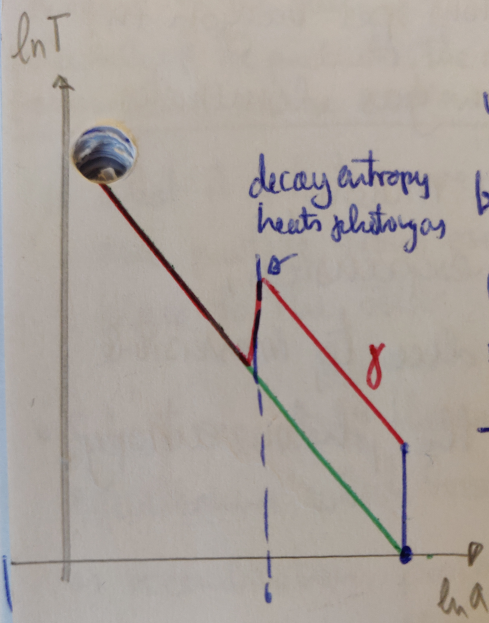
\includegraphics[width=0.5\linewidth]{gfx/neutrinoPhotonTemperature}
	\caption{}
	\label{fig:neutrinophotontemperature}
\end{figure}

\begin{mybox}{Temperature of photon and neutrino gas}
The temperature of the photon gas is therefore higher than that of the neutrino gas
\begin{equation}
\label{eq:photonAndneutrinoTemperature}
	T_\gamma = \left(\frac{11}{4}\right)^{\frac{1}{3}} T_\nu \approx 1.4 T_\nu,\quad \begin{array}{ll}
	T_\gamma = 2.726 K & \text{photons}\\
	T_\nu =1.95 K & \text{neutrinos} \\
	\end{array}.
\end{equation}
Hence the photon temperature is approx. $40\%$ higher today than the neutrino temperature.
\end{mybox}
\vspace{1cm}
What is then the contribution of the CNB to the full radiation energy density today $\Omega_{r,0,tot}$ ? \\
We know
\begin{equation*}
u \propto T^4\qquad \Omega_{r,0,\gamma}\approx 4\times10^{-5}
\end{equation*}
where the latter fact is from measurements. Including the statistical weights from neutrinos, we therefore have to replace
\begin{equation*}
	u_\gamma \rightarrow u_\gamma + \underbrace{3}_{species} \overbrace{\frac{7}{8}}^{=\frac{g_F}{g_B}\; fermion} \underbrace{\left(\frac{4}{11}\right)^{\frac{4}{3}}}_{\ref{eq:photonAndneutrinoTemperature}}u_\gamma = u_\gamma \left[1+\frac{21}{8} \left(\frac{4}{11}\right)^{\frac{4}{3}}\right].
\end{equation*}
Therefore, the neutrino contribution is given by
\begin{equation}
\Omega_{r,0,tot} = \Omega_{r,0,\gamma}\left[1+\frac{21}{8} \left(\frac{4}{11}\right)^{\frac{4}{3}}\right].
\end{equation}

\subsubsection{Photons and Baryons}
Baryons are non-rel. and therefore due to the Boltzmann suppression $n_B \propto e^{-T}$, much fewer in number than the relativistic species.\\
The number density of baryons $n_B$ and of photons $n_\gamma$ both scale with temperature $n_B,n_\gamma \propto T^3\propto a^{-3}$\footnote{Note that temperature of the universe means temperature of the photon gas and vice versa.}, hence their ratio $\eta$ \textbf{is constant}
\begin{equation}
	\eta = \frac{n_B}{n_\gamma} = 2.7 \times 10^{-8} \Omega_B h^2
\end{equation}
with
\begin{equation}
	n_B \propto \frac{\rho_B}{m_p}= \frac{\Omega_B}{m_p} \frac{3 H^2_0}{8 \pi \mG} = 1.1 \times 10^{-5} \underbrace{\Omega_B h^2}_{\approx 0.025} \;cm^{-3}
\end{equation}\footnote{assuming baryons are locked up in hydrogen}
and today
\begin{equation}
	n_\gamma=n_\gamma(T_{CMB}) =407 \; cm^{-3}.
\end{equation}
Thus, there are approximately a billion photons per baryon in the universe. The entropy of the photon gas dominates the entropy of the universe by a huge margin, justifying the assumption of adiabatic expansion, because any contribution to the entropy due to irreversible processes can be neglected compared to the photon entropy.




\subsubsection{The Recombination process}
The early universe was opaque to electromagnetic radiation, because of (Thomson) scattering by free electrons, as the mean free path each photon could travel before encountering an electron was very short. As the temperature drops, electrons and protons combine to form hydrogen atoms when the reaction
\begin{equation}
e^- + p^+ \leftrightharpoons H + \gamma 
\end{equation}
freezes out. This happens, because at lower temperature there are less high energetic photons to scatter the free electrons or to destroy the new hydrogen atoms. Then the photons decouple from matter, as their mean free path grew rapidly and became longer than the horizon distance. Then $e^-$ and $p^+$ recombine to hydrogen and the photons travel freely through the universe from there on known as \emph{cosmic microwave background} (CMB).\\
Before recombination, the strongest coupling between the photons and the rest of the plasma is through Thomson scattering
\begin{equation}
e^- + \gamma \rightarrow e^- + \gamma.
\end{equation}
The sharp drop in the free electron density after recombination means that this process becomes inefficient and the photons decouple.\\
\\
At what temperature did the freeze-out happen ?\\
We make the following approximations for this analysis:
\begin{enumerate}
	\item Overall number of particles stays fixed, i.e. canonical ensemble.
	\item All species are classical ideal gases composed of indistinguishable particles with densities low enough for degeneracy effects to be negligible.
	\item The photons do not contribute because they provide the heat bath controlling the temperature $T$.
	\item The inter-particle separation $\gg \lambda_B$ of particles involved, thus it is valid to compute the classical partition sum in phase space.
	\item The chemical potential must vanish in chemical equilibrium (compare \ref{eq:chemicalpotential})
	\begin{equation}
		\mu_e + \mu_p =  \mu_H,
	\end{equation}
	thus we have the Massenwirkungs-law in thermal equilibrium
	\begin{equation}
		\frac{Z_e Z_p}{Z_H} = \frac{N^2_e}{N_B - N_e}.s
	\end{equation}
\end{enumerate}
\begin{mybox}{Saha equation}
	We arrive at Saha's equation\begin{equation}
		\frac{x^2}{1-x} = \frac{(2 \pi m_e k_B T)^{\frac{3}{2}}}{(2\pi \hbar)^3 n_B} e^{-\frac{\chi}{k_B T}}
	\end{equation}
	with ionisation potential of hydrogen 
	\begin{equation}
		\chi = (m_e+m_p-m_H) c^2 = 13.6 eV
	\end{equation}
	and $x=\frac{N_e}{N_B}$ the \emph{ionisation degree} or \emph{free electron fraction}. 
\end{mybox}
\begin{figure}[h!]
	\centering
	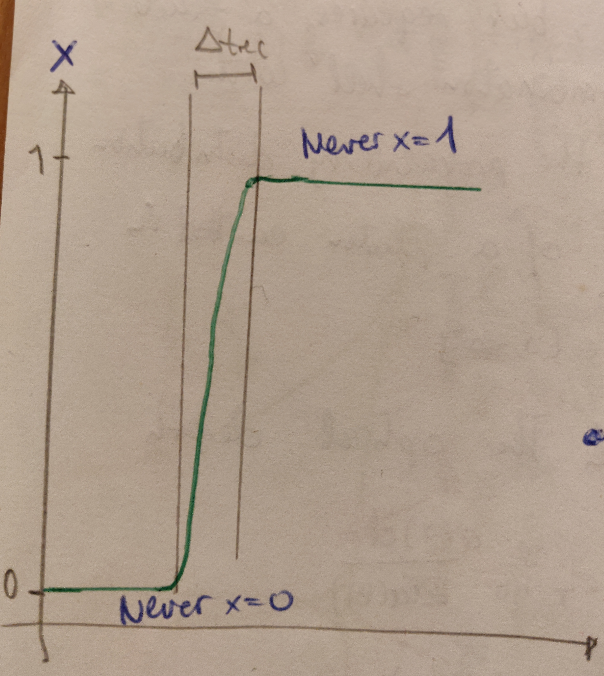
\includegraphics[width=0.5\linewidth]{gfx/sahaeq}
	\caption{}
	\label{fig:sahaeq}
\end{figure}



\begin{mybox}{Recombination epoch}
	This equation tells us that photons decoupled from matter at approximately
	\begin{equation}
	T_{rec} \approx 3400K.
	\end{equation}
	Since $\chi=13.6 eV$, one would naively expect $T_{rec} \approx10^5 K$. The very large photon-to-baryon ration $\eta^{-1}$ delays recombination considerably\footnote{Due to the Wien tail in the planck distribution of photons.}\\
	Once recombination starts, it happens very fast in a time period of approximately
	\begin{equation}
		\Delta t_{rec} \approx 40000 yr \quad \Leftrightarrow \quad \Delta z = 200.
	\end{equation}
	With $T_0 \approx 2.7K$ and $T_{rec}$ we find the scale factor at which recombination happened by noting that for ultra-rel. particles
	\begin{equation}
		T\propto a^{-1} \; \Rightarrow \; T =\frac{T_0}{a},\;\Leftrightarrow T_{rec} = \frac{T_0}{a_{rec}},
	\end{equation}
	which gives us (as $a_0=1$)
	\begin{equation}
		a_{rec} = \frac{T_0}{T_{rec}} \approx \frac{1}{1200}, \; z_{rec} \approx 1320, \; t_{rec} \approx 380000yrs
	\end{equation}
	after the Big Bang. With matter-radiation equality at $z_{eq} \approx 3500$, we conclude that \textbf{recombination occurred in the matter-dominated era}.
\end{mybox}\footnote{One has to include the $60\%$ neutrino contribution in CMB for correct results.}
Note the following comments on the recombination epoch:
\begin{enumerate} 
\item Note that Saha's equation assumes thermal equilibrium which breaks down as recombination proceeds. Still, it provides a very good approximation as $\Delta t_{rec}$ os very brief.
\item 
Why do we only see approx. one temperature of the decoupled photons, i.e. of the CMB ?\\
The photons released earlier at higher temperature are redshifted for a longer duration $\Rightarrow$ This evens the decoupled photons out in temperature such that all photons released at recombination arrive at the same energy, the same temperature today.
\item 
The Recombination process is also delayed by the following process:\\
Freshly formed hydrogen atoms can be ionized again by the recombination energy, by photons emitted from just then forming hydrogen atoms. The recombination energy is at least a Lyman-$\alpha$-photon and thus very energetic. Recombination can only proceed from this point onwards due to forbidden two-photon processes (e.g. $2s\rightarrow1s$).
\end{enumerate}
On the finite time-width of the Recombination epoch:\\
Recombination is not instantaneous, but requires a finite time interval. There is thus a \emph{recombination shell} with finite thickness. This can be analysed as follows. Imagine a photon escaping the cosmic plasma after being scattered off of an electron for the last time at a redshift depth $z$ inside the recombination shell (i.e. $Z$ corresponds to some geometrical depth $L$). One can quantify the probability distribution for last scattering at redshift $z$ of a photon emitted in the recombination shell
\begin{figure}[h!]
	\centering
	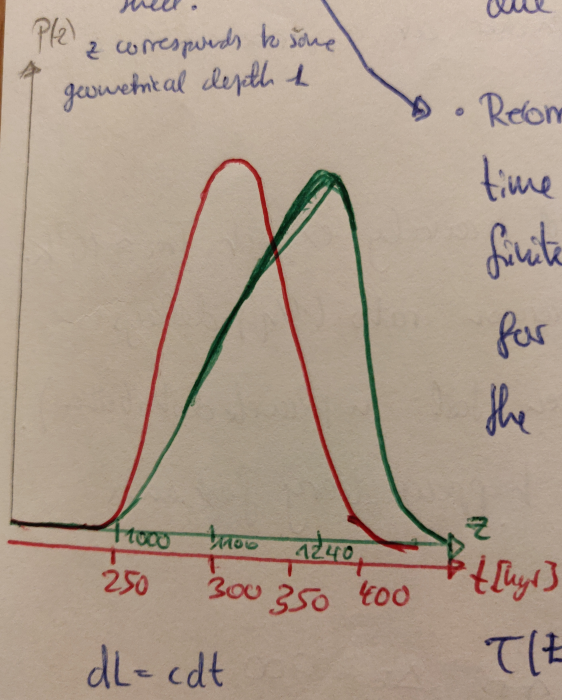
\includegraphics[width=0.5\linewidth]{gfx/RecombinationShell1}
	\caption{}
	\label{fig:recombinationshell1}
\end{figure}


\begin{equation}
	\frac{\md P(z)}{\md z} = \frac{\md \tau(z)}{\md z} e^{-\tau(z)},\qquad \tau \in[0,\infty] 
\end{equation}
with the \emph{optical depth} along a light ray in the recombination shell
\begin{equation}
	\tau(z) = n_e \sigma \int \md r = n_B \sigma T \int x \md r= - \int n_{B_0} (1+z)^3 [T_0 (1+z)] \sigma_T \frac{c}{H_0} \frac{a(z) \md z}{E[a(z)]}.
\end{equation}\footnote{The Thickness of the recombination shell is $\sigma_Z \approx 130$.}
The recombination shell is respective area as the backward lightcone (compare \ref{fig:recombinationshell}).
This $ \tau(z)$ is the optical depth of the recombination shell in the way that you ask how far you can go back into the recombination shell and find an electron that scatters on a photon for the last time. The probability distributions is Gaussian and centred around $z=1200$.
\begin{figure}[h!]
	\centering
	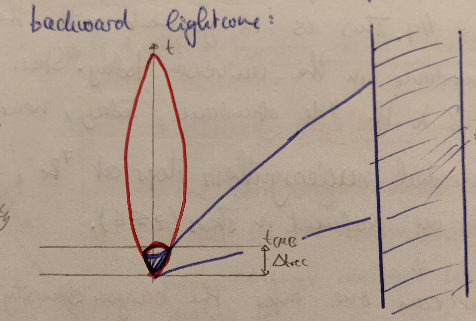
\includegraphics[width=0.5\linewidth]{gfx/recombinationShell}
	\caption{}
	\label{fig:recombinationshell}
\end{figure}
This shell is all the photons we see emitted in recombination. Thus, the probability for last scattering decreased exponentially after the recombination. The finite width of the recombination shell also shows, that the CMB photons were emitted at different $z$, as explained above they arrive all at the same redshift nevertheless.

\subsubsection{Nucleosynthesis}
Photons get hotter going back in time. This implies that there was a period of \emph{primordial nucleosynthesis} 
\footnote{Note for this analysis that the total number of nucleons stays constant due to baryon number conservation.}.\\
Photons and neutron are in thermal equilibrium until the reactions
\begin{equation}
	n+\nu_e \leftrightharpoons p+e^-,\quad n+e^+ \leftrightharpoons p+\bar{\nu}_e
\end{equation}
freeze out at $k_B T\approx 800 keV$. At this point, protons are way more common than neutrons, because neutrons are heavier. Until they're locked up again in $d, {}^4 He$ fusion processes at about $k_B T \approx 80 keV$, the neutrons decay furthermore, such that the neutron-to-proton ratio drops to
\begin{equation}
	\frac{n_n}{n_p}=\frac{1}{5} e^{-\frac{t}{\tau_n}} |_{t=5\text{ min}} = \frac{1}{7}
\end{equation}\footnote{Boltzmann distribution for decay of neutrons, takes $5$ mins. Protons and neutrons don't have the same number density in thermal equilibrium.}
\marginpar{$\tau_n=890 s$}
because neutrons decay for approximately $5$min until deuterium fusion sets in.
\begin{mybox}{Deuterium bottleneck}
	High photon density prevents ${}^2 H$ formation through photo dissociation until temperature has dropped well below $k_B T \approx 2$MeV corresponding to the binding energy. ${}^2 H$ formation is delayed until $k_B T\approx 80$keV at about three minutes after the Big Bang.
\end{mybox}
\begin{figure}[h!]
	\centering
	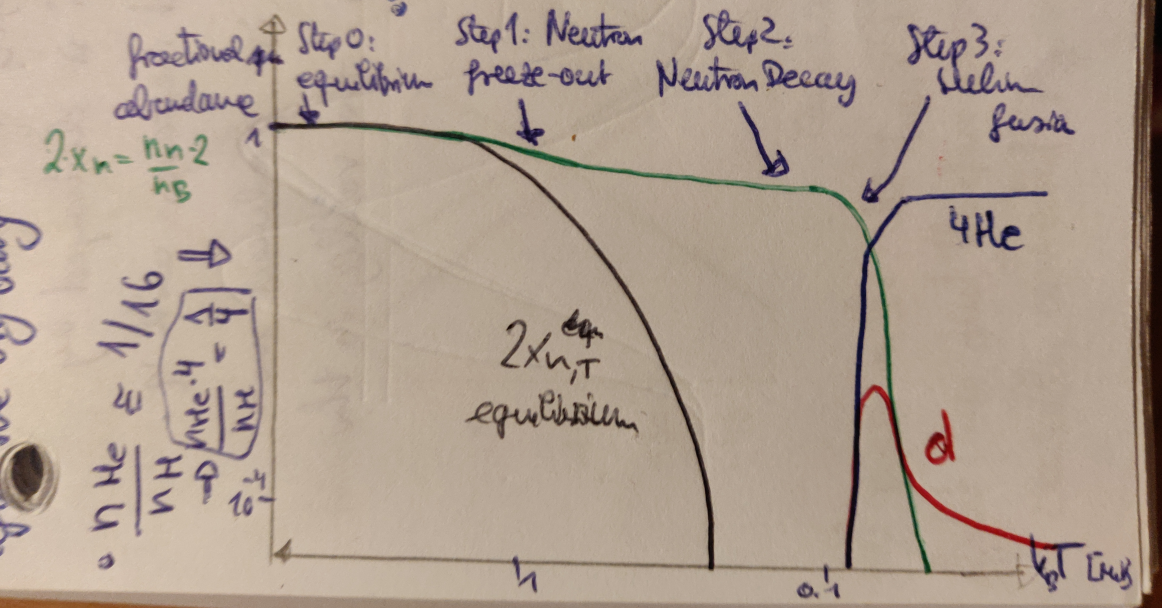
\includegraphics[width=0.5\linewidth]{gfx/nucleosynthesis}
	\caption{}
	\label{fig:nucleosynthesis}
\end{figure}
Big Bang nucleosynthesis began roughly $10$ seconds after the big bang, when the universe had cooled sufficiently to allow deuterium nuclei to survive disruption by high-energy photons (the neutron-proton freeze out time was earlier). At this point all free neutrons get locked up through a fusion chain into ${}^4 He$ because of its high binding energy. The expected ${}^4 He$ abundance by mass is $Y_P = \frac{1}{4}$ \footnote{$\frac{n_{He}}{n_H} \approx \frac{1}{16}$ implying $\frac{4 \cdot n_{He}}{n_H} = \frac{1}{4}$.}. This is in agreement with the measurement of ${}^4 He$ abundance in the universe today. Stars have only contributed $\approx 4\%$ to the ${}^4 He$ abundance today, nearly only primordial abundance.\\
Primordial nucleosynthesis stops at ${}^7 Be$, heavier elements are later on produced in stars ($z\leq 6$).
\begin{figure}[h!]
	\centering
	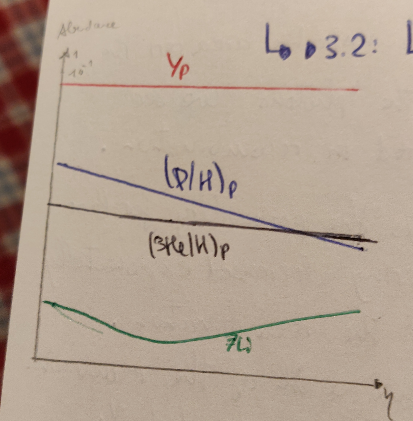
\includegraphics[width=0.5\linewidth]{gfx/nucleosynthesisAbundance}
	\caption{}
	\label{fig:nucleosynthesisabundance}
\end{figure}
\begin{mybox}{Lithium valley}
Description of \ref{fig:nucleosynthesisabundance}:\\
The abundance of ${}^4He$ increases with increasing $\eta$ as nucleosynthesis starts earlier for larger baryon density. $D$ and ${}^3 He$ are burnt by fusion, thus their abundances decrease as $\eta$ increases. Finally, ${}^7 Li$ is destroyed by protons at low $\eta$ with an efficiency that increases with $\eta$. On the other hand, its precursor ${}^7 Be$ is produced more efficiently as $\eta$ increases. This explains the \emph{Lithium valley} in the curve for ${}^7 Li$.
\end{mybox}
\vspace{1cm}
How can one infer the baryon density $\Omega_B$ of the universe from light element abundances ?\\
The abundances of light elements like helium, deuterium and lithium depend on the baryon-to-photon ratio $\eta$ which depends on the baryon density $\Omega_B$. Since deuterium has the strongest dependence on $\eta$, it gives the tightest constraints on $\Omega_B$.\\
Comparison with observations is difficult because light elements get produced and consumed (e.g. in stars) during cosmic history. Objects need to be found which either retain the primordial element mix, or in which abundance changes can be constrained.




























\newpage
\section{Cosmological Inflation}
\subsection{The horizon and flatness problem}
\subsubsection{Horizon problem}
The comoving radius of a sphere around a given point in the recombination shell which could have had causal contact with this point before recombination is
\begin{equation}
	\Delta \omega(0,t_{rec}) \approx 200 Mpc.
\end{equation}
The angular diameter-distance from us to the recombination shell is 
\begin{equation}
	D_{ang}(0,z_{rec}) \approx 6 Mpc.
\end{equation}
Thus, the angular size of the particle horizon \emph{at recombination} on the CMB sky is therefore
\begin{equation}
	\theta_{rec} = \frac{a_{rec} \Delta \omega(0,a_{rec})}{D_{ang}(0,a_{rec})} \approx 1.7^°.
\end{equation}
Given any point on the microwave sky, the causally connected region around it has a radius of approximately one degree.
\emph{How is it possible that the CMB is nearly isotropic ? Points on the sky further apart than $\approx 2^°$ had no chance of causally interacting and ’communicating’ their temperature}. This constitutes the \emph{Horizon problem}.\\
\\
From another POV, we can consider the Horizon problem via an analysis of our past lightcone, compare \ref{fig:horizonproblem}.
\begin{figure}[h!]
	\centering
	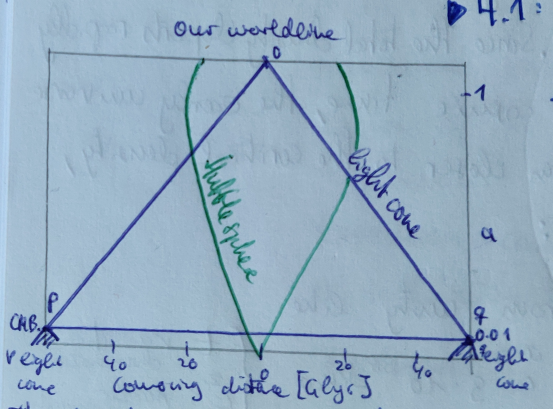
\includegraphics[width=0.7\linewidth]{gfx/horizonproblem}
	\caption{}
	\label{fig:horizonproblem}
\end{figure}
 The intersection of our past ligt cone with the spacelike slice labelled CMB corresponds to two opposite points in the observed CMB. their past light cones do not overlap before they hit the singularity $a=0$, so the points never have been in causal contact. The same applies to any two points in the CMB that are separated by more than $1$ degree on the sky.
\\
\\
This problem, as well as the Flatness problem as we will see below, can be solved by a period of inflation. Note that cosmological inflation is a model, it is proposed to solve these and other conundrums, but we have yet to measure the slow-roll parameters successfully, nothing is set in stone as of yet.\\
Inflation implies a phase of shrinking Hubble radius\footnote{The Hubble radius $r_H =\frac{c}{aH}$ is the comoving distance over which particles can travel in the course of one expansion time (the expansion time is the Hubble time $t_H = H^{-1} = \frac{\md t}{\md \ln a}\propto$ the time in which $a$ doubles).}. 
The past light cones of widely separated points in the CMB now (i.e. after a period of cosmological inflation) had enough time to intersect before $t=0$.



\begin{figure}[h!]
	\centering
	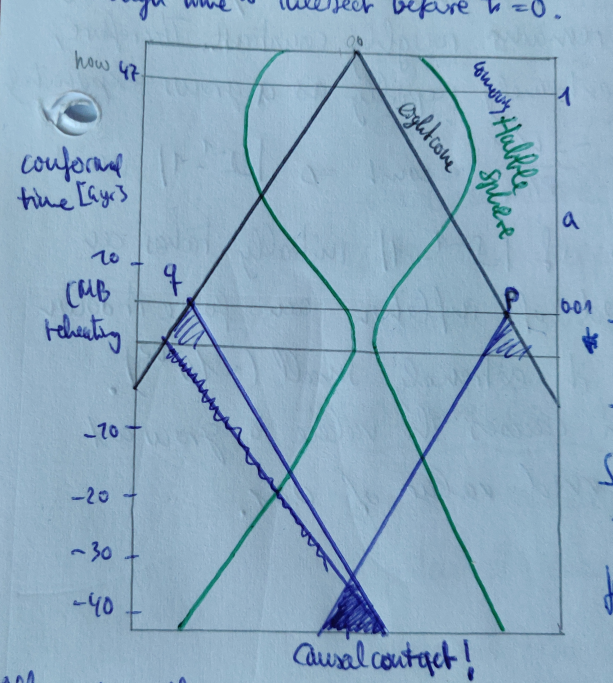
\includegraphics[width=0.7\linewidth]{gfx/Inflation}
	\caption{}
	\label{fig:inflation}
\end{figure}
All points in the CMB now have overlapping past light cones and therefore originated from a causally connected region of space.\\
\begin{mybox}{Idea of inflation}
	Summarizing, inflation is a mechanism to achieve 
	\begin{equation}
		\omega_{ph} \gg \frac{c}{a H} = r_H
	\end{equation}
	such that particles can not communicate now (or when CMB was created), but were in causal contact early on.
\end{mybox}


\subsubsection{Flatness problem}
This problem constitutes the fact that the spatial curvature of the universe is fine-tuned to a very special value and that small deviations from this value would have an extreme effect on the appearance of the universe.  The current density of the universe is observed to be very close to the critical value $\rho_{cr}$ required for flat universe. Since the total density departs rapidly from the critical value after cosmic time, the early universe must have had a density even closer to the critical density, departing from it by $\propto 10^{-62}$:
\\
The total density deviates from unity like
\begin{equation}
	\abs{1-\Omega_{tot}} = \frac{K c^2}{a^2 H^2(a)} \stackrel{a=a_{eq}}{\approx} 3\cdot 10^{-58} \Omega_{K,0} \; \left\{\begin{array}{ll}
	t & \text{radiation domination} \\
	t^{\frac{2}{3}} & \text{matter domination} \\
	\end{array}		\right\}.
\end{equation}
If there is any tiny deviation of $\Omega_{total}$ from unity at early times, it moves rapidly away from unity. In order for $\Omega_{total}$ to be anywhere near unity today, it must have been extremely close to unity at early times, which constitutes a \emph{fine-tuning problem}.
\\
Inflation provides a possible solution:\\
The proposed cause of inflation is a field which permeates spacetime and drives the expansion. the field contains a certain energy density, but unlike the density of matter or radiation present in the late universe, which decreases over time, the density of the inflationary field remains roughly constant. Therefore, the term $\rho a^2$ increases extremely rapidly as $a$ grows exponentially with
\begin{equation}
\left( \frac{1}{\Omega}-1  \right)\rho a^2 = -\frac{3 K c^2}{8 \pi \mG} = const. 
\end{equation}
$\Rightarrow \; \abs{\Omega^{-1}-1}$ must decrease with time. Thus, if $\abs{\Omega^{-1}-1}$ initially takes an arbitrary value, a period of inflation can force it down towards $0$ and leave it extremely small ($\approx 10^{-62}$). Subsequent evolution then causes the value to grow and bring it to the today observed value of $0.01$.

\subsection{The idea of inflation}
Accelerated expansions seems incompatible with gravity because the gravitational force exerted by the matter inside a representative spherical section of the universe is expected to decelerate its expansion.\\
Expansion can accelerate, i.e. $\ddot{a}>0$, if and only if the pressure is sufficiently negative
\begin{equation}
\stackrel{\ref{eq:friedmanneq2}}{\Rightarrow} \quad p< - \frac{\rho c^2}{3}.
\end{equation}
This is equivalent to shrinking the comoving Hubble radius
\begin{equation}
	\frac{\md}{\md t} \left(\frac{c}{a H}\right) <0.
\end{equation}
Thus, the idea of inflation also solves the flatness problem, because it could be solved if the comoving Hubble radius could shrink sufficiently for some time \footnote{The statement that our universe is expanding is equivalent to the statement that our field of view is getting narrower.}, because then the deviation of $\Omega_{total}$ from unity would be driven towards zero.\\ The Hubble radius characterizes the radius of the observable universe, thus the comoving Hubble radius gives the radius of the observable universe in comoving coordinates. If the comoving Hubble radius could shrink during some time, the observable part of the universe could be moved within causally connected regions, thus the contents of the entire observable universe could be brought into causal contact. After this phase ends, the observable universe can expand again, but its physical state can appear coherent everywhere thereafter, thus posing a solution to the horizon problem.
\subsubsection{Slow-Roll conditions for inflation to happen}
In this model, inflation ocurred by a scalar field rolling down a potential energy hill. When the field rolls very slowly compared to the expansion of the universe, inflation occurs. However, when the hill becomes steeper, inflation ends and reheating can occur.\\
Assume the inflaton field to be a scalar field with a finlaton potential $V(\phi)$, which has to be nearly constant
\begin{align}
	\mL &= - \half g^{\alpha \beta} \partial_\alpha \phi \partial_\beta \phi - V(\phi) \\
	\Rightarrow \quad T\munu&=\partial_\mu \phi \partial_\nu \phi+g\munu \left[-\half g^{\alpha \beta} \partial_\alpha \phi \partial_\beta \phi - V(\phi)\right]
\end{align}
with the total inflaton energy density
\begin{equation}
	\rho_\phi = \half \dot{\phi}^2 + V(\phi).
\end{equation}
The requirement for accelerated expansion resulted in the need for \textbf{negative pressure} 
\begin{equation}
\ddot{a} >0 \quad \Rightarrow \quad p < -\frac{\rho c^2}{3}.
\end{equation}
How do you get this ? For the inflaton field introduced, this can be achieved, if it satisfied the following conditions
\begin{align}
	\frac{\dot{\phi}^2}{\hbar c^3} & \ll V \text{ $\phi$ has to move sufficiently slow}\label{eq:slowroll1}\\
	\ddot{\phi} & \ll \frac{\md V(\phi)}{\md \phi}.\label{eq:slowroll2}
\end{align}
These imply for the equation of state $P = w \rho  c^2$:
\begin{equation}
	w= \frac{\frac{\dot{\phi}^2}{2 \hbar c^3} -  V}{\frac{\dot{\phi}^2}{2 \hbar c^3} + V}
\end{equation}
which has the lower bound $w\rightarrow -1 $ for a still standing field $\frac{\md \phi}{\md t}=0$. Thus, with the condition \ref{eq:slowroll1} $w$ gets sufficiently negative and we arrive at negative pressure, thus repulsive gravity.\\
\\
A successful inflationary phase (the conditions stated above) can be phrased in terms of the conditions for the slow-roll parameters.
\marginpar{$E_{pl} = m_{pl} c^2 = \sqrt{\frac{\hbar c^5}{\mG}}$, $V^\prime := \frac{\md V(\phi)}{\md \phi}$}
\begin{mybox}{Slow-roll conditions}
\begin{enumerate}
	\item Inflation occurs only if the kinetic energy $\frac{\dot{\phi}^2}{2}$ only makes a small contribution to the total energy $\rho_\phi$:
	\begin{equation}
\epsilon := \frac{E^2_{pl}}{16 \pi \mG} \left( \frac{V^\prime}{V}\right)^2 \ll 1.
	\end{equation}
	This condition says, that the slope of the potential has to be small in comparison to the potential. This reads as $V\approx$constant during inflation, i.e. during inflation the Hubble function is essentially constant
	\begin{equation}
		H\approx \text{constant} !
	\end{equation}
	The $\epsilon$ condition is needed for an inflation epoch to start in the first place.
	\item 
	\begin{equation}
		\eta := \frac{E^2_{pl}}{8 \pi \mG} \left(\frac{V^{\prime \prime} }{V}\right) \ll 1.
	\end{equation}
	This condition says that $V$ is essentially flat w.r.t. $\phi$. Thus it says that the first conditions has to hold for a long time. This conditions is needed for an inflation epoch to last.
\end{enumerate}
\end{mybox}
The condition that the two slow-roll parameters $\epsilon$ and $\eta$ be much smaller than unity indicates that both the slope and the curvature of the inflaton potential have to be small in order to generate a substantial negative pressure that results in a period of accelerated expansions that is strong enough and that lasts long enough in order to solve both the horizon and flatness problem.\\
\\
Thus with $H(a)\approx$constant during inflation, the comoving Hubble radius $\frac{c}{aH}$ has to shrink during this epoch, because $a$ increases with time. This was the required criterion to solve the flatness problem. By an estimate in order for inflation to solve the flatness problem, the comoving Hubble radius had to shrink by $\approx 10^30$, which corresponds to an increase in the scale factor by approximately $e^{60}$. This solves the causality problem at the same time, because before inflation one has a tiny patch of observable domains in thermal equilibrium which is then inflated exponentially. Then one ends up with an observable universe which appears to be in thermal equilibrium.\\
\\
Since th densities of observable quantities scale like $\rho_r \propto a^{-4}$, $\rho_m \propto a^{-3}$, all other densities than the energy density of the inflaton field (which is approximately constant during inflation, since $\rho c^2 \approx V$ and the changes in $V$ are small due to slow-roll conditions) drop by huge amounts.\\
 Since there is matter and radiation in the universe today, there must a way to convert the energy density of the inflaton field into the energy density of radiation or matter as inflation ends, i.e. when $(\epsilon,\eta)\approx 1$.\\
 It is assumed that the inflaton field can decay through some coupling to ordinary matter and thus turn its energy density back into other constituents of the cosmic fluid $\Rightarrow$ \emph{reheating process}. \textbf{This is an open question}.

\subsubsection{Inflation and structure formation}
Once inflation sets in, the vacuum fluctuations of the inflaton field due to the uncertainty principle are quickly driven outside of the horizon (i.e. the horizon quickly contracts below the length scale of the quantum fluctuations), where they "freeze in" because they lack causal contact.\\
\paragraph{Idea of Inflation originating cosmic structures}
Like any other quantum field, the inflaton field must have undergone microscopic vacuum fluctuations due to Heisenberg's uncertainty relation. As inflation started, the wavelengths of these fluctuations grew so large that they became larger than the horizon at that time\footnote{In terms of comoving distance, the particle horizon is equal to the conformal time $\eta$ that has passed since the Big Bang.}. As a result, thee now largely microscopic fluctuations lose their causal connection, cannot decay any more and therefore freeze in. These fluctuations then serve as a seed for the structures in the Universe that we can observe today.\\
\\
The model for density fluctuations produced in this way is described crudely in the following:
\begin{enumerate}
	\item Introduce a conformal time $\md \eta$ for the inflationary epoch, i.e. $\eta \in (-\infty,0)=$ (beginning inflation, end inflation). With $H\approx constant$ during inflation one finds
	\begin{equation*}
		\md s^2 = a^2(\eta) \left[-\md \eta^2 + \md \vec{\omega}^2\right] \quad \Rightarrow \quad a \md \eta = c \md t
	\end{equation*}
	such that
	\begin{equation*}
		\eta = - \frac{c}{H a} \quad [\md \eta] = \text{length} \Rightarrow \; \mathcal{H} (\eta):= \frac{a}{c} H.
	\end{equation*}
\item Make a mean field ansatz for the inflaton field by decomposing it into a smooth part $\varphi_c$ and a part $\varphi$ responsible for fluctuations
\begin{equation}
	\varphi \rightarrow \phi_c + \varphi.
\end{equation}
Fluctuations of the field imply fluctuations of the metric. By Einsteins equations one finds a modified Poisson equation
\begin{equation}
	\frac{\md^2 u}{\md \eta^2} - \frac{\left(\frac{\md^2 z}{\md \eta^2}\right)}{z} u - \vec{\nabla}^2 u = 0,\quad z= \frac{a^2}{a^\prime}\phi^\prime_c,\; u=a \varphi + \phi z.
\end{equation}
By imposing the slow-roll conditions and only perturbing to the $1^{st}$ order, one can approximate this field equation. One finds a free mode expansion of the field $u\approx a \varphi$, thus of the fluctuations, by this approximation ($V$ is assumed to be nearly constant). The solution through a Fourier transform reads
\begin{equation*}
	u^\pm_k = u^{(0)}_k e^{\pm i k \eta} \left(1 \pm \frac{i}{k \eta}\right) \; \Rightarrow \; \varphi^\pm_k = \varphi^{(0)}_k \frac{H}{ck} e^{\pm i k \eta} \left[i \pm k \eta\right].
\end{equation*}
These are the inflaton fluctuations, \emph{Bunch-Davies modes}.
\item With this result, one can make the case distinction
\begin{mybox}{}
	\begin{enumerate}
		\item $\abs{k \eta} \ll 1 \Rightarrow \varphi^\pm_k\approx constant$ (i.e. freeze-in) \emph{and} $\lambda \gg$ Horizon ($\frac{k c}{H} \ll 1$).
		\item $\abs{k \eta} \gg 1 \Rightarrow \varphi^\pm_k$ oscillating very fast \emph{and} $\lambda \ll$ Horizon ($\frac{k c}{H} \gg 1$).
	\end{enumerate}
\end{mybox}
\item Thus, by the exponential expansion of inflation, $k$ grows greatly beyond the horizon. In the horizon, the modes oscillate and they freeze-in after being driven out of the horizon. Thus in the horizon inflaton and anti-inflaton particles are causally connected, such that they recombine and fluctuations disappear. They are no longer causally connected outside of the horizon, such that they cannot recombine anymore and the fluctuations stay after being driven out of horizon. Then, out of horizon with $\lambda \gg$Horizon, the inflaton fluctuations are 
\begin{equation*}
	\tilde{\varphi}^\pm_k=\varphi^{(0)}_k \frac{H(t_X)}{c k},
\end{equation*}
where $t_X$ is the time of modes crossing the horizon.
\item In order to estimate the size of the remaining fluctuations outside of the horizon one has to evaluate the amplitude of the field. This can be done via the vacuum expectation value of the inflaton field
\begin{equation}
\expval{\tilde{\varphi}^\pm_k}{0} = \varphi^{(0)}_k= \frac{E^{\frac{3}{2}}_{pl}}{\sqrt{2 \hbar c k} }.
\end{equation}
Then the amplitude of which inflaton modes on average freeze out as they leave the horizon is then
 \begin{equation}
 	\expval{\abs{\tilde{\varphi}^\pm_k}^2}{0} = \frac{E^3_{pl}}{2 \hbar c^3} \frac{H(t_X)}{k^3}, \quad H(t_X)\approx H_k.
 \end{equation}
 \item In the next step one wants to find the \emph{(primordial) density power spectrum}. Therefore one wants to derive a relation between the density fluctuations, Fourier modes and the fluctuations today. Thus something like 
 \begin{equation*}
 	(\text{inflaton fluctuations}(k))\propto (\text{cosmic density fluctuations}(k)).
 \end{equation*}
One finds
\begin{equation}
	\delta := \frac{\delta \rho}{\rho} = \frac{2 \cdot 16 \pi}{E^2_{pl}} \frac{V}{\frac{\md V}{\md \varphi_c}} \cdot \varphi. 
\end{equation}
Therefore the amplitude of mean density fluctuations is 
\begin{equation}
	\expval{\abs{\left(\frac{\delta \rho}{\rho}\right)_k}^2}{0} = \frac{4}{3} \frac{1}{E_{pl}} \frac{V}{k^3 \epsilon} |_{k=a H},
\end{equation}
which is evaluated at the time where modes with $k$ crossed the horizon and freezes in.\\
Therefore we find that the density fluctuations depend on $k$, i.e. they have a defined spectrum. This is the \emph{density power spectrum} $P(k)$, which says how much of the signal (e.g. of CMB) is at wavenumber $k$
\begin{equation}
	P(k)=\abs{\hat{\delta}(\vec{k}) }^2.
\end{equation}
\paragraph{Comment on matter power spectrum, may remove later if added in structure formation}
The matter power spectrum describes the density contrast of the universe (the difference between local and mean density) as a function of scale. It is the Fourier transform of the matter correlation function. On large scales, gravity competes with cosmic expansion and structures grow according to linear theory. In this regime, the density contrast field is Gaussian, Fourier modes evolve independently, and the power spectrum is sufficient to completely describe the density field. On small scales, gravitational collapse is non-linear, and can only be computed accurately using $N$-body simulations.
\item The scalar power spectrum is formally defined as
\begin{equation}
\mathcal{P}_S := \frac{k^3}{2 \pi^2} \expval{\left(\frac{\delta \rho}{\rho}\right)^2_k}.
\end{equation}
\item The modes caused by the inflationary expansion of quantum fluctuations are called \emph{scalar modes}. Their power spectrum is with the above result
\begin{equation}
	\mathcal{P}_S = \frac{2}{3\pi^2 E_{pl}} \left(\frac{V}{\epsilon}\right)_{k=aH},
\end{equation}
again evaluated at the point when modes left horizon.
\item This scalar power spectrum has an exponent close to one
\begin{equation}
	\frac{\md \ln \mathcal{P}_S}{\md \ln k} = - 6 \epsilon +2 \eta \equiv n_s -1 \quad \Rightarrow\quad P_S = A k^{n_s}, \; A=const.
\end{equation}
The index of $\mathcal{P}_S,n_s$, can now be measured, thus a linear combination of the slow-roll parameters can be measured, this is one possibility to test inflation.
\item Fluctuations in the inflation field result in fluctuations in the metric. This results in gravitational waves, the so-called tensor-modes. Thus, the tensor modes also have a power spectrum
\begin{align}
	\mathcal{P}_t &= \frac{3^2}{\epsilon \pi^2 E_{pl}} V|_{k=aH} = \tilde{A}k^{n_t} = \tilde{A} k^{-2 \epsilon} \nonumber \\
	\Rightarrow \quad \frac{\md \ln \mathcal{P}_t}{\md \ln k} &= -2 \epsilon \equiv n_t \nonumber \\
	\Rightarrow \quad \frac{\mathcal{P_t}}{\mathcal{P}_s} &=16 \epsilon =: r.
\end{align}
\item Thus there are three quantities measurable to prove inflation
\begin{align}
	n_s &= 2 \eta - 6 \epsilon +1 \\
	n_t &= -2 \epsilon\\
	r&= 16 \epsilon.
\end{align}
\begin{mybox}{How to validate Inflation}
	Inflation makes the following observable predictions
	\begin{enumerate}
		\item The initial scalar perturbations should have a nearly Gaussian nature. This was confirmed with the temperature fluctuations in CMB.
		\item The scalar perturbations should have a spectral index, that is almost unity. Its deviation from unity is given by a combination of the slow-roll parameters. This small deviation from unity was actually observed.
		\item Primordial gravitational waves with an almost flat spectrum are predicted; their spectral index should be given by $-2 \epsilon = n_t$.
		\item The ration between tensor and scalar perturbations should be given by $16\epsilon =r$.
	\end{enumerate}
	Until now, primordial gravitational waves have not yet been observed without a doubt.
\end{mybox}

\end{enumerate}


















\subsection{Dark Energy}
What is the mechanism that drives accelerated expansion of the Universe today ?\\
Two possible forms
\begin{enumerate}
	\item One form of dark energy could be the cosmological constant, representing a constant energy density filling space homogeneously.
	\item A quantum scalar field, dynamic quantities whose energy density can vary in time and space. One possibility is the \emph{quintessence field}.
\end{enumerate}
Comments on the above possibilities are in order.
\subsubsection{On inflation as dark energy}
It is not possible to regard the inflaton as the driving mechanism of accelerated expansion today, because it decayed at the end of inflation.
\subsubsection{On the role of dark energy as byproduct of the universe or of dark energy}
The occurence of $\Lambda$ and $\mG$ in a $4$-dimensional metric theory of gravity is perfectly natural as explained by Lovelock's theorem.
\subsubsection{Self-interacting scalar field}
A self-interacting scalar field would produce the negative pressure necessary for accelerated expansion
\begin{equation}
w= \frac{\frac{\dot{\phi}^2}{2 \hbar c^3} -  V}{\frac{\dot{\phi}^2}{2 \hbar c^3} + V}.
\end{equation}
One suggestion for the interaction potential of quintessence is the \emph{Ratra-Peebles potential}
\begin{equation}
	V(\phi) = \kappa \left(\frac{\phi_0}{\phi}\right)^\alpha.
\end{equation}
We find that for $\alpha > -2$ this quintessence field dominates at late times and leads to accelerated expansion. This RP. potential is favourable because of its \emph{tracker properties}: A wide variety of initial conditions for $\phi,\dot{\phi}$ lead to the same final solution for $\phi$.\\
\\
In all these possible models one has to consider time dependent equation of state parameters as well, such as
\begin{equation}
	w=w_0 +(1-a) w_a,
\end{equation}
which is called \emph{CPL-parametrization}. One observes \begin{equation}
	(w_0,w_a) \approx (-1,0)
\end{equation}
today (which is cosmological constant), a clear deviation would imply that accelerated expansion is \emph{not} driven by the cosmological constant.


\section{Evolution of cosmic structures}

\subsection{Linear perturbation theory}
Here we describe the basic theory for structure growth in the expanding universe. With the inhomogeneities being much smaller than the typical scale of the universe, we can neglect effects of GR/curvature and finite speed of information propagation and work with Newtonian dynamics and classical Hydrodynamics (fluid approximation).\\
We thus describe inhomogeneities in a cosmic fluid\footnote{Ideal fluids here, i.e. set of mass points with infinitely small mean free path (obvs. not true for cosmic fluids, but ok approximation in large scale regime).} which contains at least radiation, dark and baryonic matter and which moves according to Newtonian gravity:\footnote{Consider thus a non-relativistic fluid with mass density $\rho$, pressure $P\ll \rho$ and velocity $\vec{v}$.}
\begin{mybox}{Euler-Poisson equations}
	Energy-momentum conservation of a cosmic fluid $\partial_\mu T^{\mu \nu}=0$ is stated by the Euler-Poisson equations
	\begin{align}
		\frac{\partial \rho}{\partial t} + \vec{\nabla} \cdot (\rho \vec{v}) &= 0 \quad \text{mass conservation} \\
		\frac{\partial \vec{v}}{\partial t} + (\vec{v}\cdot \vec{\nabla}) \vec{v} &= - \frac{\vec{\nabla} P}{\rho} - \vec{\nabla}\Phi \text{  momentum conservation}\\
		\vec{\nabla}^2 \Phi &= 4 \pi \mG \rho.
	\end{align}
\end{mybox}
We want to find such a set of equations solely for the fluctuations parts of the $\rho,\vec{v}$ fields. We hence decompose the velocity and density field into their homogeneous background values, indicated by subscript $0$, and small perturbations

\begin{equation}
	\rho = \rho_0 (1+\delta), \; \vec{v}=\vec{v}_0+a \vec{u}, \; \Phi=\Phi_0+\phi.
\end{equation}
These are given in \emph{comoving coordinates} $\vec{r}=a(t) \vec{x}$, i.e.
\begin{equation*}
	\frac{\md}{\md t}(a \vec{x}) = \underbrace{\dot{a} \vec{x}}_{\text{Hubble flow}} + \underbrace{a \dot{\vec{x}}}_{\text{peculiar velocity}}
\end{equation*}
with the \emph{relative density contrast}
\begin{equation}
	\label{eq:densitycontrast}
	\delta = \frac{\delta \rho}{\rho}.
\end{equation}
\begin{mybox}{Linear perturbation equations}
	By only considering perturbations up to first order we find three perturbation equations
	\begin{align}
		(C) \quad \dot{\delta}+\vec{\nabla}\cdot \vec{u} &=0\\
		(E) \quad \dot{\vec{u}} + 2 H \vec{u} &= - \frac{\vec{\nabla}P}{a^2 \rho_0} - \frac{\vec{\nabla}\phi}{a^2} \\
		(P) \quad \vec{\nabla}^2 \phi &= 4 \pi \mG \rho_0 \delta a^2\\
		&\Leftrightarrow \frac{\delta \hat{\phi}}{c^2}=-\frac{3}{2} \frac{k^2_0\hat{\delta}}{k^2 a} |_{k^2_0\equiv\Omega_{K,0}H^2_0/c^2},
	\end{align}
where $(C)$ implies that particles must stream together to form density correlations.
\end{mybox}
We find an equation of state linking the pressure fluctuations to the density fluctuations
\begin{equation}
	 P=c^2_s \rho_0 \delta,
\end{equation}
\footnote{Not exactly correct, because $c_s$ has to be taken under adiabatic conditions, an adiabatic index is missing here.}
where $c_s=0$ for linearized CDM fluctuations.

\subsubsection{Density perturbations}
By combination of the perturbation equations one finds
\begin{align}
\ddot{\delta}+ 2 H \dot{\delta} &= \left[4 \pi \mG \rho_0 + \frac{c^2_s}{a^2} \vec{\nabla}^2\right]\delta,\\
\ddot{\delta}_k + 2 H \dot{\delta}_k &= \left[4 \pi \mG \rho_0 - \frac{c^2_s k^2}{a^2}\right]\delta_k, \nonumber \\
 \text{using       } \delta(\vec{x},t) &= \int \frac{\md^3 k}{(2 \pi)^3} \delta_k(\vec{k},t) e^{-i \vec{k}\cdot \vec{x}}\nonumber.
\end{align}
\begin{enumerate}
	\item One finds a d'Alembert equation for sound waves by dropping $\dot{\delta}$ and gravity term.
	\item By dropping $\dot{\delta}$ and $\vec{\nabla}^2$ one finds an exponentially growing oscillator, this describes the growth of cosmic structure.
\end{enumerate}
$2H \dot{\delta}$ is a damping term guaranteeing that cosmic structure growth goes as a power law, not exponentially. In case $1)$ this damping term dissipates the sound waves.

Below Jean's length, the fluctuations oscillate with decreasing amplitude. Above the Jeans' length, the fluctuations experience power-law growth, rather than exponential growth due to the damping term.





























\subsection{Linear growth factor, perturbations within and outside the horizon}
\subsection{Velocity perturbations and Zel'dovich approximation}
\subsection{Nonlinear evolution and power spectra}
\subsection{The Cosmic Microwave Background}
\subsubsection{The Dipole}
\begin{mybox}{}
	The Earth is not at rest with respect to the CMB.
\end{mybox}
Its motion around the Sun, combined with the Sun's motion around the centre of the Milky way, and so on, causes an effective net motion with velocity $v$ with respect to the CMB.
\begin{mybox}{CMB Dipole}
	This motion causes a dipolar pattern in the CMB temperature,\begin{equation}
		T_{obs} = T_{CMB,0} \left[1+\frac{v}{c} \mu\right] + \mathcal{O}\left(\frac{v^2}{c^2}\right), \quad \mu = \cos\angle(\vec{n},\vec{v}).
	\end{equation}
	The amplitude of the Dipole is, with the Earth's velocity being $v_{Earth} \approx 371 \frac{km}{s}$,
	\begin{equation*}
		T(v_{Earth}) \approx 10^{-3}K.
	\end{equation*}
\end{mybox}
The cosine of the angle between the line-of-sight and the direction of motion. The CMB temperature is slightly enhanced towards the direction of motion, and decreased in its anti-direction, corresponding to the Doppler shift of CMB photons.\\
Thus, one has to remove the mean value/background noise of the galactic plane and everything else and the Dipole from the CMB measurement to find the bare CMB with fluctuations of
\begin{equation}
	\frac{\Delta T}{T} \approx 10^{-5}.
\end{equation}
The density contrast at decoupling was of the order $\delta(a_{CMB}) \approx 10^{-3}$, we would therefore expect the CMB fluctuations to be of order $10^{-3}K$. The observed order of $10^{-5}K$ can be explained through the existence of not electromagnetically interacting dark matter.
\subsubsection{Perturbation equations and the Sachs-Wolfe effect}
Regarding initially only the ultra-rel CMB photons, we have
\begin{align}
	n &\propto T^3, \quad u \propto T^4, \quad P=\frac{u}{3} \propto T^4 \\
	\Rightarrow \quad \frac{\delta n}{n_0}& = 3 \theta,\quad \frac{\delta u}{u_0} = \frac{\delta p}{p_0} = 4\theta.
\end{align}
with the \emph{relative temperature fluctuation} $\theta=\frac{\delta T}{T_0}$.\\
From this we find using the continuity and Euler equation
\begin{align}
\ddot{\theta} -\frac{c^2}{3} \vec{\nabla}^2 \theta - \frac{1}{3} \vec{\nabla}^2\delta \phi &=0 \\
\ddot{\theta}_K + \frac{c^2 k^2}{3} \theta_k + \frac{k^2}{3} \delta \phi_k &=0.
\end{align}


 \todo{To finish.}




\section{Gravitational Lensing}
\subsection{Gravitational Lensing Equation from GR}
\subsection{Thin gravitational lenses}
\subsection{Correlation functions (no thin lens approximation)}
\section{Theoretical Astrophysics}








\newpage
\section{Two examples of Relativistic Astrophysics}
\subsection{Gravitational Lensing - TO COMPLETE FROM SCRIPT}
Consider a congruence/bundle of geodesics and calculate the propagation of light in the vicinity of a mass in order to quantify the effects of gravitational lensing. Pick a fiducial light ray from the light bundle with a normal vector $n$ perpendicular to its four-velocity measuring the distance to the other light rays in the bundle, i.e. its amplitude measure the diameter of the cross section of the light bundle.\\

\begin{figure}
	\centering
	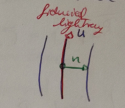
\includegraphics[width=0.7\linewidth]{gfx/gravlensingLightcongruence}
	\caption{}
	\label{fig:gravlensinglightcongruence}
\end{figure}
The Jacobi equation of geodesic equation reads:
\begin{equation}
\nabla^2_u n = \bar{R}(u,n)u.
\end{equation}
For a lightray introduce an affine parameter parametrizing the geodesic, since $\tau=0$ for light. Now, for a bundle of null-geodesics with the wavevector $\tilde{k}$ of the fiducial light ray:
\begin{equation}
\nabla^2_{\tilde{k}} n = \bar{R}(\tilde{k},n)\tilde{k},
\end{equation}
i.e. \emph{light bundles are deformed by the gravitational tidal field.}\\
\\
Note: Observer moving with $u_0$ seeing lightray measures frequency $\omega_0=\langle k, u_0 \rangle$, with $\tilde{k}:= \frac{k}{\omega_0}$.\\
\\
\subsubsection{Introduction of 2d Sachs space}
construct coordinate space $\perp \tilde{k}$ and also $\perp u_0 \Rightarrow$ 2d space in 3 space of observer, where it is perpendicular to lightray $\Rightarrow$ 2d screen perpendicular to light ray. $E_1,E_2$ span screen at the observer. Shift along lightray by parallel transport: $\nabla_{\tilde{k}}E_i=0$ and $\langle E^i,E_j \rangle = \delta^i_j; i,j \in \{1,2\}$, the \emph{Sachs basis}.\\
\begin{figure}
	\centering
	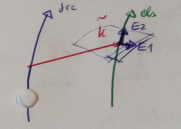
\includegraphics[width=0.7\linewidth]{gfx/gravlensingSachsbasis}
	\caption{}
	\label{fig:gravlensingsachsbasis}
\end{figure}

Also $\tilde{k} \propto k $ null: $\langle \tilde{k},\tilde{k} \rangle =0$ and null geodesics $\nabla_{\tilde{k}} \tilde{k} =0$. With $n = N^i E_i$ inserted into the geodesic deviation equation
\begin{equation}
\nabla^2_{\tilde{k}} N^i =\underbrace{ \langle E^i, \bar{R}(\tilde{k},E_j) \tilde{k} \rangle}_{=R_{\alpha \beta \gamma \delta} E^{i \alpha} \tilde{k}^{\beta} \tilde{k}^{\gamma} E^{\delta}_g} N^j .
\end{equation}
\begin{mybox}{Split up Riemann tensor }
	\begin{equation}
	\bar{R}_{\alpha \beta \gamma \delta} = \bar{C}_{\alpha \beta \gamma \delta} + g_{\alpha [\gamma} R_{\delta ] \beta} - g_{\beta [\gamma} R_{\delta] \alpha} - \frac{\mathcal{R}}{3} g_{\alpha [\gamma} g_{\delta] \beta}.
	\end{equation}
	The Weyl tensor $\bar{C}_{\dots}$ is equal to the Riemann tensor the vacuum solution of Einstein equations. It tells you which freedom you have in the Riemann tensor if you fix the Ricci tensor. The Weyl tensor is trace-free. The Weyl tensor corresponds to the gravitational tidal field and gives us the freedom left in geometry for fixed Ricci:
	\begin{equation}
	\bar{C}^{\alpha}_{\beta \alpha \delta} = 0, \quad \bar{C}_{\alpha \beta \gamma \delta} = - \bar{C}_{\beta \alpha \gamma \delta} = - \bar{C}_{\alpha \beta \delta \gamma}= \bar{C}_{\gamma\delta \alpha \beta}.
	\end{equation}
	One of the most important properties of the Weyl tensor is that it is invariant under conformal transformations. This means that if you compute $\bar{C}_{ρσμν}$ for some metric $g_{μν}$ , and then
	compute it again for a metric given by $Ω^2 (x) g_{μν}$ , where $Ω(x)$ is an arbitrary nonvanishing
	function of spacetime, you get the same answer. For this reason it is often known as the
	“conformal tensor.”
	The Weyl tensor vanishes in a homogeneous and isotropic universe, since it otherwise would induce a preferred direction. The Weyl tensor is responsible for distortions of the light bundle, which can not take place in an isotropic and homogeneous universe $\Rightarrow$ split up background and non-background action on light bundle.
	Note:
	\begin{equation}
	\phi_{ij} \rightarrow \phi_{ij} - \delta_{ij}\tr \phi_{ij} \frac{1}{3} = \underbrace{\phi_{ij}- \frac{4 \pi \rho}{3} \rho \delta_{ij}}_{\propto \bar{C}}
	\end{equation}
	which corresponds to a tidal field without matter (in Newtonian analogy). Note that the term $\propto \rho$ is the local matter. It describes the matter distribution around a light bundle as if beam were empty.
\end{mybox}
Inserting this form of the Riemann tensor into the geodesic deviation equation yields the optical tidal matrix $\mathcal{T}$:
\begin{equation}
\nabla^2_{\tilde{k}} N^i = \left[-\half R(\tilde{k},\tilde{k})\delta^i_j + \underbrace{C^i_j}_{\bar{C}_{\alpha \beta \gamma \delta} E^{i\alpha} \tilde{k}^{\beta} \tilde{k}^{\gamma} E^{\delta}_j} \right],
\end{equation}
where the former terms leads to an isotropic contraction or expansion of the light bundle cross section:
\begin{equation}
\nabla^2_{\tilde{k}} \vec{N} = \mathcal{T} \vec{N}.
\end{equation}
The Weyl tensor completely vanishes in an isotropic and homogeneous universe. Not perfect Friedmann universe $\Rightarrow$ We have fluctuations around the background which lead to Weyl fluctuations. Here , the Weyl tensor can be projected onto the tidal field of the Newtonian gravitational potential.\\
What happens for a light-bundle travelling through an unperturbed Friedmann universe ? $\Rightarrow \bar{C}=0$, i.e. ignore \emph{gravitational shear} (e.g. circular sections won't become elliptic. Ellipsis are not allowed in a Friedmann universe).
\subsubsection{Circular light bundle}
For circular light bundle (will remain circular since $C=0$). Check script for the case of $\bar{C}\neq 0$.
\begin{equation}
\nabla^2_{\tilde{k}} D = \kappa D.
\end{equation}
Expressing the Ricci tensor i.t.o. the Einstein tensor and field equation
\begin{equation}
R(\tilde{k},\tilde{k}) = G(\tilde{k}, \tilde{k}) = \frac{8 \pi \mathcal{G}}{c^4} T(\tilde{k},\tilde{k}), \quad with\, g(\tilde{k},\tilde{k})=\tilde{k}^2=0
\end{equation}
shows that the cosmological constant doesn't contribute to the propagation of light ray/bundle.\\
\\
Study light propagation in late cosmological epochs $\Rightarrow p\approx 0$:
\begin{equation}
T(\tilde{k},\tilde{k}) \approx \rho c^2 (u^{\flat} \otimes u^{\flat})(\tilde{k},\tilde{k}) = \rho c^2 (\underbrace{\langle u,\tilde{k} \rangle}_{1+z=\frac{\langle u,\tilde{k}\rangle_{src}}{\langle u, \tilde{k}\rangle_0} = \langle u,\tilde{k}\rangle_{src}}  )^2 = \rho  c^2 (1+z)^2 = \rho_0 c^2 a^{-5}.
\end{equation}
This yields $\kappa = - \frac{4 \pi \mathcal{G}}{c^2 a^5} \rho_0$ for the RHS. \\
As for the LHS, what is the curve parameter $\lambda$ running along the light ray ? $\tau=0$ for light $\Rightarrow$ introduce \emph{affine parameter} $\lambda$ parametrizing the null geodesic:
\begin{equation}
\tilde{k} = \frac{\md x^{\mu}}{\md \lambda}
\end{equation}
which defines $\lambda$ (one could also define $\lambda$ via $k= \frac{\md x^{\mu}}{\md \lambda}$, which linearly scales $\lambda\Rightarrow$ affine transformation, would be a different $\lambda$). \\
We had $\langle \underbrace{u}_{u_{obs}},\tilde{k} \rangle = 1$, or $\langle u, \tilde{k} \rangle = 1+z$ for any $u$.\\
Object moving only with cosmic flow: $u$ only has time coordinate $u = \partial_t$ in adapted coordinates: $\langle u, \tilde{k} \rangle = \tilde{k}^0$:
\begin{equation}
\tilde{k}^0 = c \frac{\md t}{\md \lambda} \quad \Rightarrow \quad \md \lambda = \frac{1}{1+z} c \md t = a c \md t 
\end{equation}
the curve parameter we have to introduce such that the normalization condition is satisfied, could introduce other.\\
From FLRW metric and radial light ray we also get $\md \lambda = a^2\md \omega$,
where we took the positive root branch since a radial comoving light ray should grow positively in time.\\
\\
Now 
\begin{equation}
\nabla_{\tilde{k}} D = \frac{\md x^{\alpha}}{\md \lambda} \partial_{\alpha} D = \frac{\md D}{\md \lambda} \; \Rightarrow\; \frac{\md^2 D}{\md \lambda^2} =\kappa D,
\end{equation}
which is not an oscillator since $kappa$ is not a constant. For the \emph{comoving bundle diameter} $\frac{D}{a}$ we on the other hand find an oscillator equation:
\begin{equation}
\frac{\md^2 }{\md \omega^2} \left(\frac{D}{a}\right) = - k \left(\frac{D}{a}\right).
\end{equation}
Thus, light propagation in an unperturbed Friedmann equation is subject to oscillating perturbations with a $\sqrt{k}$ frequency, i.e. for $k>0$ has trigonometric solutions, a \emph{positively curved space focusses light rays} (e.g. two lines going from North to South pole).\\
This leads to complications in Cosmology with distance measurements. For $k<0$ one gets hyperbolic solutions, which lead to a defocussing effect, light bundles diverge. In flat space on the other hand $k=0$, a light bundle grows linearly with the distance.\\
The background universe for $k>0$ has positive focussing effect on light bundles. This propagation equation is the starting point for gravitational lensing, to find its Greens function and integration with perturbations along the light propagation path.\\
Gravitational lensing is astigmatic (An optical system with astigmatism is one where rays that propagate in two perpendicular planes have different foci. If an optical system with astigmatism is used to form an image of a cross, the vertical and horizontal lines will be in sharp focus at two different distances), i.e. there is blurred image and betrays perturbations of universe, i.e. our knowledge of it.


\section{Tolman-Oppenheimer-Volkoff solution}
(Note that Oppenheimer-Snyder paper $\Rightarrow$ complete collapse of a star as result of Einstein field equations.)
Fill the stationary, spherically symmetric vacuum solution with matter of an ideal fluid. The matter content could now as well be relativistic: $p=\frac{1}{3} \rho c^2$ in the ultra-rel. limit. Here, energy content contained in pressure can act as a source of gravity. This is main difference to classical treatment, where pressure solely stabilizes star against gravity. In classical physics, the hydrostatic equation is $\frac{\nabla p}{\rho} = - \nabla \phi$. What is the equivalent to this in relativity ?
\\
The relativistic hydrodynamical equations for a metric connection $\nabla g=0$ 
\begin{equation}
\nabla \cdot T= u \left[u(\rho c^2 + p) + (\rho c^2+p) (\nabla \cdot u) \right] + (\rho c^2 + p) \nabla_u u+ \md p^{\sharp} = 0
\end{equation}
where $\nabla_u u=0$ for a geodesic, but fluid particles are not freely falling since they are subject to pressure. Note further that $\langle u, \nabla_u u\rangle = \half \nabla_u \langle u,u \rangle =0$, thus $\nabla_u u \perp u$. Can isolate contributions $\parallel$to $u$ which yields the \emph{relativistic continuity equation} (time-derivative of observer moving with that particular four velocity)
\begin{equation}
u(\rho c^2 +p) + (\rho c^2+p) \nabla \cdot u + u(p) = 0,
\end{equation}	
which says that the sum of energy density and pressure is continuous, and $\perp u$ with the projector $\pi^{\perp} = \mathcal{I}_4 + u \otimes u^{\flat}$, the \emph{relativistic Euler equation}
\begin{equation}
(\rho c^2+p) \nabla_u u + \md p^{\sharp} + u \cdot u(p) = 0.
\end{equation}
\subsubsection{Equivalent treatment of hydrodynamic equations and solution of a fluid in hydrostatic equilibrium - Weinberg}
In the absence of gravitation, the energy-momentum tensor of a perfect fluid is given by
\begin{equation}
T^{\alpha \beta} = p \eta^{\alpha \beta} + (p + \rho ) U^\alpha U^\beta. 
\end{equation}
The contravariant tensor that reduces to this in the absence of gravitation is
\begin{equation}
T^{\mu \nu} = p g^{\mu \nu} + (p + \rho) U^\mu U^\nu,
\end{equation}
where $U^\mu$ is the local value of $\md x^\mu/\md \tau$ for a comoving fluid element. This expression is obtained by the Principle of General Covariance. Note that $p$ and $\rho$ are always defined as the pressure and energy density measured by an observer in a locally inertial frame that happens to be moving with the fluid at the instant of measurement, and are therefore scalars. The condition of energy-momentum conservation give the hydrodynamic equations
\begin{equation}
0=T^{\mu \nu}_{;\nu} = \frac{\partial p}{\partial x^\nu} g^{\mu \nu} + g^{- \half} \frac{\partial}{\partial x^\nu} g^\half (p+\rho) U^\mu U^\nu + \Gamma^\mu_{\nu \lambda} (p +\rho) U^\nu U^\lambda.
\end{equation}
The last term represents the gravitational force on the system. Note also that since $\eta_{\alpha \beta}U^\alpha U^\beta =-1$ in the absence of gravitation, we must in the presence of gravitation have
\begin{equation}
g\munu U^\mu U^\nu =-1.
\end{equation}
Consider as an example the case of a fluid in hydrostatic equilibrium. Since it is not moving, the normalization of the four velocity gives
\begin{equation}
U^0 = (- g_{00})^{- \half} \quad U^\lambda=0 \quad for \; \lambda\neq 0.
\end{equation}
Furthermore, all temporal derivatives of $g\munu, p,$ or $\rho$ vanish. In particular,
\begin{equation}
\Gamma^\mu_{00} = - \half g^{\mu \nu} \frac{\partial g_{00}}{\partial x^\nu}
\end{equation}
and
\begin{equation}
\frac{\partial}{\partial x^\nu} \left[(p+\rho) U^\mu U^\nu\right]=0.
\end{equation}
Multiplying the hydrodynamical equations by $g\munu$ gives then
\begin{equation}
-\frac{\partial p}{\partial x^\lambda}=(p+\rho) \frac{\partial}{\partial x^\lambda} \ln(\sqrt{-g_{00}}).
\end{equation}
This is trivial for $\lambda=0$, whereas for $\lambda$ spacelike it is nothing but the ordinary non relativistic equation of hydrostatic equilibrium, except that $p+\rho$ appears instead of the mass density, and $\ln\sqrt{-g_{00}} $appears instead of the gravitational potential. This equation is soluble if $p$ is given as a function of $\rho$, hence for an e.o.s. We then find that
\begin{equation}
\int \frac{\md p(\rho)}{p(\rho) + \rho} = - \ln \sqrt{-g_{00}} + constant.
\end{equation}
For instance, if $p( \rho)$ is given by a power law $p(\rho) \propto \rho^N$, then the integral gives for $N\neq1$;
\begin{equation}
\frac{\rho+p}{\rho} \propto (-g_{00})^{\frac{1-N}{2N}}
\end{equation}
and for $N=1$
\begin{equation}
\rho \propto (-g_{00})^{-\frac{p+\rho}{2 p}}.
\end{equation}
This, incidentally, shows that gravitation can never produce hydrostatic equilibrium in a finite highly relativistic fluid with $p = \rho/3$, for then the eq. for $N=1$ gives
\begin{equation}
\rho \propto (-g_{00})^{-2}.
\end{equation}
Since $\rho$ must vanish outside the fluid, $g_{00}$ would have to become singular at its surface.




%
\subsubsection{Stationary solution}
For a stationary object in adapted coordinates $u=e_0 \propto \partial_t$ and $u(p)=0$ i.e. pressure can not change with time. Where is the gravitational force in the relativistic Euler equation for $u(p)=0$ ? It is in the covariant derivative: 
\begin{equation}
\nabla_u u= \langle \md u^{\alpha} + u^{\beta} \omega^{\alpha}_{\alpha}, u \rangle e_{\alpha} = u^0 \omega^1_0(u) e_1 = a^{'} e^{-b} e_1
\end{equation}
from the Schwarzschild solution, where the first equality is the \emph{geodesic equation in Cartan formalism}.\\
Since stationariness and spherical symmetry are imposed, we onl have a radial dependence $\md p^{\sharp} = (p^{'} e^{-b} \theta^1)^{\sharp} = p^{'} e^{-b} e_1$. This yields the 1-d rel. Euler equation in radial direction only for spherical symmetry
\begin{equation}
(\rho c^2+p) a^{'} e^{-b} + p^{'} e^{-b} =0.
\end{equation}
Equivalently, the rel. hydrostatic equation in stationary, spherically symmetric situation is
\begin{equation}
a^{'}= - \frac{p^{'} }{\rho c^2+p}, \, \frac{\nabla p}{\rho} = - \nabla \phi \, \Rightarrow \, \nabla p \leftrightarrow p^{'} , \, \nabla \phi \leftrightarrow a^{'}.
\end{equation}
The gravitational force accelerates not only the matter density but pressure as well. Thus, pressure has inertia ! Pressure corresponds to energy-density $\propto$ inertia. Force balance has to account for pressure inertia. Then, the gravitational force corresponds to the curvature of spacetime $a^{'}  \leftrightarrow \nabla \phi$, since $a$ quantifies deviation of the metric of flat (Minkowskian) spacetime. The Einstein equations then yield:
\begin{align}
	e^{-2b} & = 1-\frac{2m}{r},
\end{align}
where the mass is now radius dependent $m(r)=4 \pi \int_0^r \rho r^2 \md r \frac{\mathcal{G}}{c^2}$.
Furthermore
\begin{align}
	\nabla \phi = - \frac{\mathcal{G} M(r)}{r^2} \;&\leftrightarrow \quad a^{'} = \frac{4 \pi \mathcal{G}}{c^4} r e^{2b} p + \frac{m}{r} e^{2b} \\
	\frac{\nabla p}{\rho}= - \nabla \phi \; &\leftrightarrow \quad    a^{'}= -\frac{p^{'}}{\rho c^2+p}
\end{align}
the former expression for $a^{'}$ follows from the gravitational field equations and the latter from the hydrostatic equation.
\begin{mybox}{Tolman-Oppenheimer-Volkoff equation}
	In Newtonian physics you get the\emph{Lane-Emden} equation at this point, here we get the TOV-equation by equating both expressions for $a^{'} $:
	\begin{equation}
	- p^{'}=-\partial_r p = \frac{\left(m+ \frac{4\pi \mathcal{G}}{c^4} p r^3\right) (\rho c^2 +p )}{r(r-2m(r)) }
	\end{equation}
	Which describes the hydrostatic equilibrium in general relativity.
\end{mybox}
It has the following implications:
\begin{enumerate}
	\item Here pressure acts as an additional source of gravity in comparison to Newtonian physics
	\begin{equation}
	\frac{m}{r^2} \quad \mapsto \quad \frac{(m+ \dots p)}{r(r-2m)}
	\end{equation}
	\item Going from Newton to GR yields $\rho \mapsto \rho c^2 +p$, thus pressure has \emph{inertia}.
	\item $r-2m \Rightarrow$ horizon
	\item Easy solution for constant density $\rho=\rho_0=const. \Rightarrow$ e.g. density in a Neutron star $\rho_0 = \rho_N$ (highest possible density in universe), can integrate this out to get an upper limit on mass and radius of a neutron star $M=8 M_{sun}, R=10^{15}km$. Thus, with highest density you can have $\rho = \rho_N$ you can only stabilize objects up to $8 M_{sun}$, as more mass will lead to a supernova.
	\item Need e.o.s. to link $\rho$ and $p \Rightarrow$ can learn about hadronic e.o.s. by observing neutron stars.
	
\end{enumerate}

	\chapter{General Relativity as a Quantum Field Theory}
	\section{Conceptional differences- TO DO}
	\begin{enumerate}
		\item The sources of electromagnetism are conserved, and energy is conserved, which is the source of gravity. But this conversation is of a different character, since the photon is uncharged, and hence is not a source of itself, whereas the graviton has an energy content equal to $\hbar \omega$, and therefore it is itself a source of gravitons. We speak of this as \emph{the nonlinearity of the gravitational field.}
		
	\end{enumerate}
\section{On physical theories, remarks by Feynman}
\begin{statements}
	Rule of thumb about theories of physics: Theories not coming from some kind of variational principle, as as Least-Action, may be expected to eventually lead to trouble and inconsistencies.
\end{statements}
 It has happened in physical theories that although high order correction in a particular expansion are exceedingly tedious to compute, it is possible to construct a theory which sums all higher order corrections to give an answer which is accessible. \\
We shall search for a functional $F$ which is to be an action to be varied, for empirical reasons: There is apparently no successful theory which is not derivable from a variational principle which starts from a Lagrangian or a Hamiltonian function (which are equivalent). It is not certain whether the failures of non-Lagrangian theories reflect some fundamental truth about nature. It is possible that the fundamental truth may be that processes occur according to a principle of minimum phase, and that the actions of classical physics or of quantum physics are expressions for this phase which are correct to some approximation.\\
\\
\\
The proofs that we offer are not rigorous; we don't bother with the rigour because it is the facts that matter, and not the proofs. Physics can progress without the proofs, but we can't go on without the facts. The proofs are useful in that they are good exercises; if the facts are right, then the proofs are a matter of playing around with the algebra correctly.
\\
\\
The only reasonable thing a physicist can do now is to choose some of these terms as being "simpler" than others, disregard the complicated one, and see what kind of theory he has left. It is difficult to define complication in an unambiguous way; it is always possible to perform integrations by parts so that the derivatives disappear in one place and reappear in another - the simplicity which is apparent in starting from one point may not correspond to the simplicity which would result from a different starting point.


\section{How Feynman derived GR from a field theoretical approach}
Feynman did not start by postulating the Hilbert action by assumption of diffeomorphism invariance, where the route then incorporates to identify the variation of the matter action as the energy momentum tensor \ref{eq:GRenergymomentumtensor} to arrive at the full field equations, but he starts by guessing the energy-momentum tensor and refining his guesses via conservation of energy-momentum and physical assumptions of its form in order to constrain all general terms which could possibly contribute to the energy-momentum tensor.\\
\\
His steps are
\begin{enumerate}
	\item Postulate full gravity action by comparing possible terms to the QED action and using that the field of interest has to be the $(0,2)$ symmetric tensor representing the metric. It follows that:
	\begin{align}
		S &= \half \int \md V\left[h^{\mu \nu, \lambda} \bar{h}_{\mu \nu, \lambda} - 2 \bar{h}^{\mu \lambda}_{,\lambda} \bar{h}^{\;\;\,,\nu}\munu \right] \quad \mathrm{fields} \nonumber \\
		& \qquad - \int \md V \left(\lambda h\munu T^{\mu \nu}\right) \quad \mathrm{coupling term} \nonumber \\
		&\qquad \quad + S_M \quad \mathrm{matter},
	\end{align}
where the rank $(0,2)$ tensor $h\munu$ represents plane-wave gravitons 
\begin{equation}
	h\munu = e\munu \exp(i k \cdot x),
\end{equation}
$e\munu$ is a polarization tensor and one uses the following definitions
\begin{align*}
	\bar{X}\munu &= \half (X\munu + X_{\nu \mu}) - \half \eta\munu X^\sigma_\sigma,\\
	\Rightarrow \bar{h}\munu &= h\munu - \half \eta_{\mu \nu} h^\sigma_\sigma, \quad h \; symmetric \\
	h&\equiv h^\sigma_\sigma.
\end{align*}
One postulates this action by writing down all possible derivatives of the field tensor $h\munu$ in the action and combing all possible terms via symmetry of the tensor and the notation above, as well as using the gauge $\bar{h}^{\mu \sigma}_{\;\; , \sigma}=0$.
\item As for the energy-momentum tensor of matter, it is first obtained from the Lagrangian as canonical via \ref{eq:canonicalenergymomentumtensor}. 
\item Now: We have written down a total Lagrangian having a field term, a matter term, and a coupling term. We have arrived at afield equation by arranging that the divergence of the energy-momentum tensor should be identically zero. This procedure is evidently incorrect, since we have written a energy-momentum tensor which did not include the energy of the gravitational field itself. Thus, the present theory is physically untenable, since the energy of the matter is not conserved. One searches for a new tensor, (Belinfante-Rosenfeld tensor ? Or is BR only for symmetrization ?) to get conservation of energy:
\begin{equation}
\partial_\nu (T^{\mu \nu} + \chi^{\mu \nu}) = 0.
\end{equation}
The tensor $\chi$ is determined by writing it as a derivative of a functional, which should depend on the field $h\munu$ and its first order derivatives (Why ? p.75).:
\begin{equation}
\lambda \xi^{\mu \nu} = \frac{\delta F^3 [h]}{\delta h\munu},\quad ^{new}T^{\mu \nu} = \underbrace{^{old}T^{\mu \nu}}_{\equiv ^oT^{\mu \nu}} + \chi^{\mu \nu}.
\end{equation}
\item Now make an ansatz for the energy momentum tensor by comparison with electrodynamics:
\begin{equation}
	j^{\mu} (x) = e \int \md s \delta^{(4)}_D(x-z(s)) \dot{z}^\mu, \quad S_{int} = -e \int \md s A_\mu (z) \dot{z}^\mu, \quad \dot{z} = \frac{\md z}{\md s}.
\end{equation}
Such that one postulates
\begin{equation}
	^oT^{\mu \nu} (x) = m_0 \int \md s \delta^4_D(x-z(s)) \dot{z}^\mu  \dot{z}^\nu,
\end{equation}
where the resulting coupling term reads
\begin{equation}
	\lambda \int \md^4x ^oT^{\mu \nu}(x) h\munu (x) \quad = \lambda m_0 \int \md s h\munu (z) \dot{z}^\mu \dot{z}^\nu.
\end{equation}
There is a simple physical way to interpret the significance of the $\delta_D$ function in $^oT^{\mu \nu}$: it simply says that there is no interaction energy except where the particle actually is.\\
Now one computes the divergence of the old energy-momentum tensor and rewrites the resulting acceleration appearing in it via the geodesic equation to find that
\begin{equation}
	\chi^{\;\; ,\nu}_{\mu \nu}= [\sigma \nu, \mu] {}^o T^{\mu \nu} + \mathcal{O}(\lambda^2) \dots.
	\end{equation}
Now one writes $F^3$ as a sum over all possible independent products involving trilinear products of field components and two derivative indices and constrains the resulting equations via its variation w.r.t $h\munu$, which yields $\chi$ to find an explicit form for $F^3$.\\
The resulting field theory suffices the observations for perihelion precession and light deflection.
\item It has happened in physical theories that although high order correction in a particular expansion are exceedingly tedious to compute, it is possible to construct a theory which sums all higher order corrections to give an answer which is accessible. \\
\\ 
Thus we may attempt to deduce the entire expression $F=F^2+F^3+F^4+F^5+\dots$.\\
We shall search for a functional $F$ which is to be an action to be varied, for empirical reasons: There is apparently no successful theory which is not derivable from a variational principle which starts from a Lagrangian or a Hamiltonian function (which are equivalent). It is not certain whether the failures of non-Lagrangian theories reflect some fundamental truth about nature. It is possible that the fundamental truth may be that processes occur according to a principle of minimum phase, and that the actions of classical physics or of quantum physics are expressions for this phase which are correct to some approximation.\\
\\
Require
\begin{equation}
	\frac{\delta F}{\delta h\munu} = \lambda T^{\mu \nu} \; \Rightarrow \; g_{\sigma \lambda} \left(\frac{\delta F}{\delta h_{\sigma \nu}}\right)_{, \nu} + [\mu \nu,\lambda] \left(\frac{\delta F}{\delta h\munu}\right) = 0,
\end{equation}
where it was plugged into energy-momentum conservation equation and where one defined in the derivation of the geodesic equation 
\begin{equation}
	g\munu(x)=\eta_{\mu \nu} + 2 \lambda h\munu(x).
\end{equation}
There is a simplest solution (involving the smallest number of derivatives of $g\munu$, just two). We choose it. When this is done, we shall have arrived at a theory which is identical to Einstein's.
\item Now infinitesimal trafos are discussed to constrain functional for the path to the solution as indicated above. One then tries to construct such an $F$ which is invariant under infinitesimal transformations of the tensor $h\munu \rightarrow h^\prime\munu$. Or rather it is a transformation of a tensor field $g\munu(x)$ under an infinitesimal transformation of coordinates $x^\mu = x^{\prime \lambda} + \zeta^\lambda$. This is property of gauge invariance is discussed later by comparison with usual approach of constructing Einstein's GR via diffeomorphism invariance.
\item Use interesting matrix properties. For matrix $A^\prime = A+B$ and if $B$ is infinitesimal, one has
\begin{equation}
	\frac{1}{A^\prime} = \frac{1}{A} - \frac{1}{A }B \frac{1}{A} + \frac{1}{A} B \frac{1}{A} B \frac{1}{A }+\dots.
\end{equation}
Also one uses
\begin{equation}
	\det A = \exp(\tr \log(A)),
\end{equation}
where the latter comes about by using
\begin{equation}
	\det A = A_{11} A_{22} A_{33} \dots = \exp(\log(A_{11})+\log(A_{22})+\dots) = e^{\tr(\log(A))}. 
\end{equation}
Together they give
\begin{equation}
	\det\left[A\left(1+\frac{1}{A}B\right)\right] = \dots = \det(A) e^{\tr(\frac{1}{A}B)}.
\end{equation}
Furthermore, one constrains the solutions to be independent of the infinitesimal transformation.  Define $g^{\tau \sigma} [\mu \nu,\sigma] = \Gamma^\tau\munu$. Then one eliminates the appearing gauge objects appearing by virtue of the infinitesimal trafo by manipulating derivatives of Christoffles and introducing a tensor
\begin{equation}
	\bar{R}^\tau_{\mu \nu \rho} = \Gamma^\tau_{\mu \nu,\rho} + \Gamma^\tau_{\rho \lambda} \Gamma^\lambda_{\mu \nu}-\Gamma^\tau_{\mu \rho, \nu}-\Gamma^\tau_{\nu \lambda} \Gamma^\lambda_{\mu \rho}.
\end{equation}
Now solving the initial diff. equation finally yields with manipulation 
\begin{equation}
	F = -\frac{1}{2 \lambda^2} \int \md \tau g^{\mu \nu} \bar{R}^\tau_{\mu \nu \tau} \sqrt{- \det(g_{\alpha \beta})}.
\end{equation}
This invariant functional $F$ is equivalent to that developed by Einstein. If we make an expansion of the functional $F$ when the gravitational fields are weak, we obtain as the leading terms the $F^2$ and $F^3$ terms of earlier consideration.\\
We therefore succeeded with the aim to construct a self-consistent theory of gravitation by means of successive logical steps guessed at by analogy.
\item The Riemann tensor $\bar{R}_{\sigma \mu \nu \rho}$ is antisymmetric for an interchange of $\nu$ and $\rho$, also antisymmetric for interchange of $\sigma$ and $\mu$, and symmetric if the pair $\sigma \mu$ is interchanged with the pair $\nu \rho$. The Ricci tensor $R\munu$ is symmetric.
\item The variation of the functional $F$ w.r.t. $g\munu$ yields
\begin{equation}
	2 \frac{\delta F}{\delta g\munu} = - \frac{1}{\lambda^2} \frac{\delta (\sqrt-g) \mathcal{R}}{\delta g\munu} = \frac{1}{\lambda^2} \sqrt{-g} \left(R^{\mu \nu} - \frac{\mathcal{R}}{2} g^{\mu \nu} \right),
\end{equation}
where
\begin{equation}
	g \equiv \det(g\munu).
\end{equation}
The last quantitiy above in parantheses is the stress energy-tensor of our theory, and it satisfies the following equation:
\begin{equation}
	g_{\sigma \lambda} T^{\mu \nu}_{, \nu} = - [\mu \nu, \sigma] T^{\mu \nu} \quad or \quad T^{\mu \nu}_{,\nu} = - \Gamma^\lambda\munu T^{\mu \nu},
\end{equation}
if substituted for $T^{\mu \nu}$ as we required it to do. That is, the full equations of the gravitational field to all order are
\begin{equation}
	\sqrt{-g} \left[R^{\mu \nu} - \frac{\mathcal{R}}{2 } g^{\mu \nu} \right] = \lambda^2 T^{\mu \nu}, \quad
	g \equiv \det(g\munu).
\end{equation}
The last quantitiy above in parantheses is the stress energy-tensor of our theory, and it satisfies the following equation:
\begin{equation}
	g_{\sigma \lambda} T^{\mu \nu}_{, \nu} = - [\mu \nu, \sigma] T^{\mu \nu} \quad or \quad T^{\mu \nu}_{,\nu} = - \Gamma^\lambda\munu T^{\mu \nu},
\end{equation}
if substituted for $T^{\mu \nu}$ as we required it to do. That is, the full equations of the gravitational field to all order are
\begin{equation}
	\sqrt{-g} \left[R^{\mu \nu} - \frac{\mathcal{R}}{2 } g^{\mu \nu} \right] = \lambda^2 T^{\mu \nu},
\end{equation}
where $T^{\mu \nu}$ is our matter energy tensor. This is the equation Einstein obtained.

\item







\end{enumerate}








It is one of the peculiar aspects of the theory of gravitation, that is has both a field interpretation and a geometrical interpretation. In any case, the fact is that a spin-two field has this geometrical interpretation; this is not something readily explainable - it is just marvellous.. The geometric interpretation is not really neccessary or essential to physics. It might be that the whole coincidence might be understood as representing some kind of gauge invariance. It might be that the relationships between these two point of view about gravity might be transparent after we discuss a third point of view, which has to do with the general properties of field theories under transformations.
\subsection{The action for matter fields in a gravitational field}
QFT on curved background..\\
In order to construct a more complete theory, we add terms to the action so as to represent all the other known fields. We write the action first in flat space, as we know it, choose the simplest form from some kind of criterion which is invariant. The requirement that the action should be invariant results in covariant equations for the fields. This is not a restriction on what known fields we can include, because all the known laws of physics can be covariantly written. Differential laws have this property. Any law written as a differential equation may easily be converted to a covariant form; we assume that in the tangent space the law it the same as the one we know, and then bring it down to the manifold. Once we have written all processes, first in differential form, then in covariant form, then we can use our theory to compute e.g. the motion of matter in a star. What is not allowed is to use laws which would violate energy conservation.
\subsection{Final formulation of Gravity on path to quantum gravity}
\begin{equation}
	\delta S_g = - \frac{1}{2 \lambda^2} \delta \int \md^4x H, \; H= \sqrt{-g} g^{\mu \nu} \left[\Gamma^\rho_{\nu\sigma} \Gamma^\sigma_{\rho \mu} - \Gamma^\rho_{\mu \nu} \Gamma^\sigma_{\rho \sigma}\right].
\end{equation}
We are now ready again to make a quantum theory, after having a theory from Einstein's point of view. The theory is more complete then when we were discussing the Venutian viewpoint (i.e. approach via energy-momentum tensor as a field theory and not via diffeomorphism invariance) -  we have the complete Lagrangians including interaction with matter correct to all orders. If we restrict our attention to a universe consisting only of gravity fields and scalar matter, the field theory is obtained by considering expansions in terms of a coupling constant
\begin{equation}
	g\munu=\eta\munu+2\lambda h\munu.
\end{equation}
In the Lagrangian, the terms which are quadratic correspond simply to the propagators, the terms involving product of two $\phi$ and one $h$, and terms involving three $h$'s and two $\phi$'s, correspond to diagrams as

\begin{figure}[h!]
	\centering
	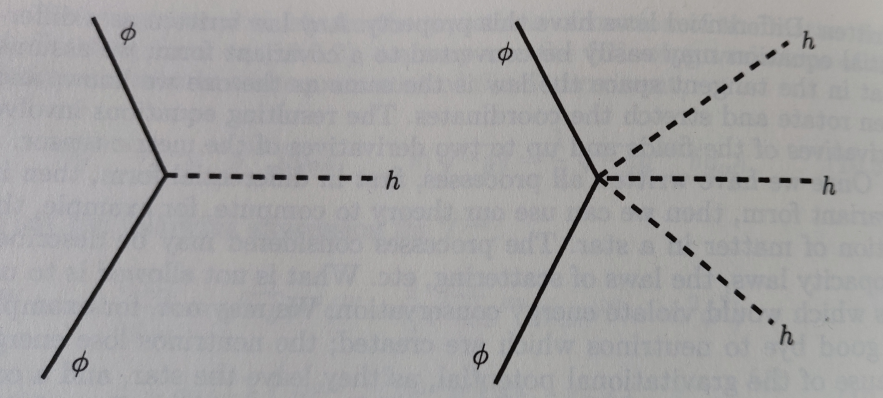
\includegraphics[width=0.7\linewidth]{gfx/feynmanquantumgravity}
	\caption{}
	\label{fig:feynmanquantumgravity}
\end{figure}
In this way, we have arrived at a prescription for calculating quantum mechanical amplitudes for the motion of matter after having started out from a geometrical point of view.\\
In considering the terms in the action, we might consider why the field term might not include a certain proportion $\Lambda$ of $\int \md^4 x \sqrt{-g}$. This would be an integral proportional to the volume of the universe, presumably a constant. The resulting equation for the field behaves somewhat as though the gravitons had a mass and a universal source. The observation of the extremely long range of gravity forces makes it rather pointless to introduce such a term (since mass would imply Yukawa cut-off ?), even though it might lead to a consistent theory. The equations of motion that come from it are
\begin{equation}
G\munu = \Lambda g\munu + \lambda^2 T\munu.
\end{equation}
The constant $\Lambda$ is known as the cosmological constant. Einstein wanted a closed universe, so he assigned to it a value which made steady-state solutions of such a universe possible. This he later referred to as hi Great Mistake; had he chosen it equal to zero, he would have concluded that the unvierse must be expanding (or contracting). 























\newpage
\chapter{Possible Exam problems}
\begin{enumerate}
	\item WAS AN EXERCISE Generalize the Schwarzschild solution for Einstein's equations with a cosmological constant.
	\item PROBABLY Determine the solution representing the spacetime outside a spherically symmetric charged body carrying an electric charge (but no spin and magnetic dipole moment). The sult is the RN sol (c=1) 
	\begin{equation}
		g = - \left(1-\frac{2m}{r} + \frac{\mG e^2}{r^2}\right) \md t^2 + \left(1 - \frac{2m}{r } + \frac{\mG e^2}{r^2}\right)^{-1} \md r^2 + r^2\md \Omega^2,
	\end{equation}
	where $m/\mG$ represents the gravitational mass and $e$ is the electric charge of the body.\\
	Solution: Since fields are static and spherically symmetric we can use for the metric the ansatz of the Schwarzschild solution 
	\begin{equation}
		g=-e^{2 a(r)} \md t^2 + e^{2 b(r)} \md r^2 + r^2\md \Omega^2.
	\end{equation}
	it is again convenient to worj in the orthonormal tetrad 
	\begin{equation}
	\theta^0 = e^a \md t,\; \theta^1= e^b \md r, \; \theta^2 = r \md \vartheta, \; \theta^3 = r\sin\vartheta \md \varphi,
	\end{equation}
	such that the metric then reads:
	\begin{equation}
		g=g\munu \theta^\mu \otimes \theta^\nu, \quad (g\munu) = \mathrm{diag}(-1,1,1,1).
	\end{equation}
	Hence we make the ansatz
	\begin{equation}
		F = \frac{e}{r^2} \theta^0 \wedge \theta^1.
	\end{equation}
	For this the components of the energy-momentum tensor are readily found to be
	\begin{equation}
		T^0_0=T^1_1=-T^2_2=-T^3_3 = -\frac{e^2}{8 \pi r^4},
	\end{equation}
	all other $T\munu =0$. Hence, the equations $G^0_0=8 \pi \mG T^0_0$ and $G^1_1= 8 \pi \mG T^1_1$ become
	\begin{align}
		\frac{1}{r^2} - e^{-2b} \left(\frac{1}{r^2} - \frac{2 b^\prime}{r}\right) &= \frac{\mG e^2}{r^4} \\
		\frac{1}{r^2} - e^{-2b} \left(\frac{1}{r^2} + \frac{2 a^\prime}{r}\right) &= \frac{\mG e^2}{r^4}.
	\end{align}
By subtraction we see that again $a*b=0$. Furthermore, $G_{00}$ equation is equivalent to
\begin{equation}
	(r e^{-2b})^\prime = 1 - \frac{e^2 \mG}{r^2}.
\end{equation}
The metric functions are thus given by
\begin{equation}
	e^{2a} = e^{-2b} = 1 - \frac{2m}{r} + \frac{e^2 \mG}{r^2},
\end{equation}
where $m$ has the same interpretation as for the Schwarzschild solution. The other components of Einstein's equation are also satisfied. It remains to show that Maxwell's vacuum equations are also fulfilled. For this we first note that $F=\md A$, $A=\frac{e}{r} \md t$, hence $\md F=0$. Since $*F=-\frac{e}{r^2} \theta^2 \wedge \theta^3=\md (e \cos \vartheta \md \varphi)$, we have also $\md * F =0$. For later use we write the result in the form
\begin{align}
	g &= - \frac{\Delta}{r^2} \md t^2 + \frac{r^2}{\Delta} \md r^2 + r^2 \md \Omega^2 \\
	F&= - \frac{e}{r^2} \md t \wedge \md r,\\
	\Delta &= r^2 - 2mr + e^2 \mG.
\end{align}
	

\item Show that the effective potential of the Schwarzschild solution has the following properties
\begin{enumerate}
	\item For $L/m < 2 \sqrt{3}$ any incoming particle falls toward $r=2m$
	\item The most tightly bound, stable circular orbit is at $r=6m$ with $L/m=2 \sqrt{3}$ and has fractional binding energy of $1-\sqrt{8/9}$.
	\item Any particle with $E\geq 1$ will be pulled into $r=2m$ if $2\sqrt{3} < L/m < 4$.
\end{enumerate}
\item Redshift Schwarzshild bh p 202 ff ?
\item Show that the Newtonian-limit metric gives the correct deflection of light rays
\item Show that the Newtonian-limit metric gives $4/3$ times the Einstein value for the perihelion precession. This demonstrates once more that the precession of the perihelion is sensitive to non-linearities in GR.
\item Maybe a gravitational waves exercise, even though never did any ?
\item 
\end{enumerate}








1 








\chapter{Important equations of GR - TO DO}
\section{Differential Geomtetry}

\section{Statements from problem sheets}
\begin{enumerate}
\item Euler-Lagrange Equations for field $\phi$
\begin{equation}
	\partial_\lambda \left[\frac{\partial \mL}{\partial(\partial_\lambda \phi)}\right] - \frac{\partial \mL}{\partial \phi} =0.
\end{equation}
For a coordinate $x^\mu$
\begin{equation}
	\frac{\md}{\md \tau} \left(\frac{\partial \mL}{\partial \dot{x}^\mu}\right) - \frac{\partial \mL}{\partial x^\mu}=0.
\end{equation}
\item Null geodesics remain null geodesics $\dot{x}^\mu \dot{x}_\mu=0$ under conformal transformation
\begin{equation}
	g \mapsto \tilde{g} = e^{2 \phi(x^\nu) } g.
\end{equation}
\item On the $S^2$ sphere, one can define forms as on every manifold. With the differential operator of codifferential and hodge-dual, one can then define a divergence or gradient on the sphere. These relations are useful in the
context of spherically symmetric solutions of Einstein’s field equations (e.g. the Schwarzschild
solution). As will be seen in the lecture, the manifold describing space-time can then be foliated
as $M^4 = M^2 × S^2$ . Operators (like the covariant divergence or the Laplacian) on the second
submanifold can be expressed elegantly by differential forms on $S^2$.
\item Note that the following expansion is independent of the metric
\begin{equation}
	\partial_\alpha \phi \partial^\alpha \phi = \partial_0 \phi \partial^0 \phi + \partial_i \phi \partial^i \phi.
\end{equation}
Only upon pulling down the index do we get metric factors in front.
\item For computations of lifetimes, distances and what not for observer near BH, use eom derived from Lagrangian, i.e. try to use the eom
\begin{equation}
	\left(\frac{\md r}{\md \tau}\right)^2 + V(r) = E^2,
\end{equation}
or the conserved quantities 
\begin{equation}
	\langle \dot{\gamma} , \partial_t\rangle = E= const. \qquad \langle \dot{\gamma},\partial_\varphi\rangle = L =const.
	\end{equation}

\item Use integration trick for integral
\begin{equation}
	\md \tau = \int_0^{2m} \frac{\md r}{\sqrt{\frac{2m}{r} -1}}
\end{equation}
thus
\begin{equation}
	r = m(1+\cos \eta),\qquad \md r = - m \sin \eta \md \eta.
\end{equation}
\item radial infall $\Rightarrow$ $\dot{\varphi}=0 \Rightarrow L=0$.
\end{enumerate}
\section{Statements to incorporate}
\begin{enumerate}
	\item The
	appearance of an effective cosmological constant makes it
	impossible to find any solutions of the Einstein field equations in which $g\munu$ is the constant Minkowski  $\eta\munu$. That is, the original symmetry of general covariance,
	which is always broken by the appearance of any given
	metric $g\munu$
	cannot, without fine-tuning, be broken in
	such a way as to preserve the subgroup of space-time
	translations.
	\item There were two things that especially attracted me to the ideas of renor-
	malization and quantum field theory. One of them was that the requirement
	that a physical theory be renormalizable is a precise and rational criterion of
	simplicity. In a sense, this requirement had been used long before the advent
	of renormalization theory. When Dirac wrote down the Dirac equation in
	1928 he could have added an extra ‘Pauli’ term 7 which would have given
	the electron an arbitrary anomalous magnetic moment. Dirac could (and perhaps did) say ‘I won’t add this term because it’s ugly and complicated
	and there’s no need for it.’ I think that in physics this approach generally
	makes good strategies but bad rationales. It’s often a good strategy to study
	simple theories before you study complicated theories because it’s easier to
	see how they work, but the purpose of physics is to find out why nature is
	the way it is, and simplicity by itself is I think never the answer.
	\item But
	why the Lagrangian formalism? Why do we enumerate possible theories by
	giving their Lagrangians rather than by writing down Hamiltonians? I think
	the reason for this is that it is only in the Lagrangian formalism (or more
	generally the action formalism) that symmetries imply the existence of Lie
	algebras of suitable quantum operators, and you need these Lie algebras to
	make sensible quantum theories. In particular, the S-matrix will be Lorentz
	invariant if there is a set of 10 sufficiently smooth operators satisfying the
	commutation relations of the inhomogeneous Lorentz group. It’s not trivial
	to write down a Hamiltonian that will give you a Lorentz invariant S-matrix
	— it’s not so easy to think of the Coulomb potential just on the basis of
	Lorentz invariance — but if you start with a Lorentz invariant Lagrangian
	density then because of Noether’s theorem the Lorentz invariance of the S-
	matrix is automatic
	\item The bottom line is that quantum me-
	chanics plus Lorentz invariance plus cluster decomposition implies quantum
	field theory.cluster decomposition principle, which requires that distant experiments give
	uncorrelated results
	\item Finally, what is the motivation for the special gauge invariant Lagrangians
	that we use in the standard model and general relativity? One possible an-
	swer is that quantum theories of mass zero, spin one particles violate Lorentz
	invariance unless the fields are coupled in a gauge invariant way, while quan-
	tum theories of mass zero, spin two particles violate Lorentz invariance unless
	the fields are coupled in a way that satisfies the equivalence principle.
	\item string theory is a two dimensional conformally invariant field theory, but not a quantum
	field theory in four spacetime dimensions.
	\item  at
	finite temperature there’s no S-matrix because particles cannot get out to
	infinite distances from a collision without bumping into things. Also, it
	seems quite possible that at very short distances the description of events in
	four-dimensional flat spacetime becomes inappropriate.
	\item The present
	educated view of the standard model, and of general relativity, 14 is again that
	these are the leading terms in effective field theories.
	\item We generally deal with gauge theories
	by choosing a gauge before quantizing the theory, which of course breaks
	the gauge invariance, so it’s not obvious how gauge invariance constrains
	the infinities. (There is a symmetry called BRST invariance 15 that survives
	gauge fixing, but that’s non-linearly realized, and non-linearly realized sym-
	metries of the action are not symmetries of the Feynman amplitudes.)
	\item  The theorem
	that says that infinities are governed by the same gauge symmetries as the
	terms in the Lagrangian was originally proved back in the old days by ’t
	Hooft and Veltman 16 and Lee and Zinn-Justin 17 only for theories that are
	renormalizable in the old power-counting sense, but this theorem has only
	recently been extended to theories of the Yang–Mills 18 or Einstein type with
	arbitrary numbers of complicated interactions that are not renormalizable in
	the power-counting sense
	\item As I have said, quantum field theories provide an expansion in powers
	of the energy of a process divided by some characteristic energy; for soft
	pions this characteristic energy is about a GeV; for superconductivity it’s
	the Debye frequency or temperature; for the standard model it’s 10 15 to 10 16
	GeV; and for gravitation it’s about 10 18 GeV. Any effective field theory loses
	its predictive power when the energy of the processes in question approaches
	the characteristic energy. So what happen to the effective field theories of
	electroweak, strong, and gravitational interactions at energies of order 10 15 –
	10 18 GeV? I know of only two plausible alternatives.
	One possibility is that the theory remains a quantum field theory, but one
	in which the finite or infinite number of renormalized couplings do not run off
	to infinity with increasing energy, but hit a fixed point of the renormalization
	group equations. One way that can happen is provided by asymptotic free-
	dom in a renormalizable theory, 25 where the fixed point is at zero coupling,
	but it’s possible to have more general fixed points with infinite numbers of
	non-zero nonrenormalizable couplings. Now, we don’t know how to calculate
	these non-zero fixed points very well, but one thing we know with fair cer-
	tainty is that the trajectories that run into a fixed point in the ultraviolet
	limit form a finite dimensional subspace of the infinite dimensional space of
	all coupling constants.That means that the condition, that the trajectories hit a fixed point, is just as restrictive in a nice way as renormalizability used to be:
	It reduces the number of free coupling parameters to a finite number.  The other possibility, which I have to admit is a priori more likely, is that
	at very high energy we will run into really new physics, not describable in
	terms of a quantum field theory
	\item There have been two fundamental insights in the development of the renor-
	malization group. One, due to Gell-Mann and Low, is that logarithms of
	energy that violate naive scaling and invalidate perturbation theory arise be-
	cause of the way that renormalized coupling constants are defined, and that
	these logarithms can be avoided by renormalizing at a sliding energy scale.
	The second fundamental insight, due to Wilson, is that it’s very important
	in dealing with phenomena at a certain energy scale to integrate out the
	physics at much higher energy scales. It seems to me these are the same
	insight, because when you adopt the Gell-Mann–Low approach and define a
	renormalized coupling at a sliding scale and use renormalization theory to
	eliminate the infinities rather than an explicit cutoff, you are in effect inte-
	grating out the higher energy degrees of freedom — the integrals converge
	because after renormalization the integrand begins to fall off rapidly at the
	energy scale at which the coupling constant is defined. (This is true whether
	or not the theory is renormalizable in the power-counting sense.) So in other
	words instead of a sharp cutoff a la Wilson, you have a soft cutoff, but it’s
	a cutoff nonetheless and it serves the same purpose of integrating out the
	short distance degrees of freedom.
	\item 
\end{enumerate}
\end{document}
% ********************************************************************
